\documentclass[diploma]{Styles/softlab-thesis}

%%%
%%%  The document
%%%

% PACKAGE SETTINGS =============================================================
\usepackage{textcomp}
\usepackage{color}
\usepackage{listings}

%----------------------------------------------------------------------------------------
%	LISTINGS (CODE) TEMPLATE4$  $
%----------------------------------------------------------------------------------------

\lstset
{
	keywordstyle=\bfseries\ttfamily\color[rgb]{0,0,1},
	identifierstyle=\ttfamily,
	commentstyle=\color[rgb]{0.133,0.545,0.133},
	stringstyle=\ttfamily\color[rgb]{0.627,0.126,0.941},
	showstringspaces=false,
	basicstyle=\small,
	numberstyle=\footnotesize,
	numbers=left,
	stepnumber=1,
	numbersep=10pt,
	tabsize=2,
	breaklines=true,
	prebreak = \raisebox{0ex}[0ex][0ex]{\ensuremath{\hookleftarrow}},
	breakatwhitespace=false,
	aboveskip={1.5\baselineskip},
  	columns=fixed,
  	upquote=true,
  	extendedchars=true,
	frame=single
	inputencoding=utf8
}



\begin{document}

%%%  Title page

\frontmatter

\title{Σχεδίαση και Υλοποίηση cloud συστήματος για εθελοντική αιμοδοσία}
\author{Φωτόπουλος Ηλίας\\Ρεβέκκα Παλαιολόγου}
\date{Σεπτέμβριος 2015}
\datedefense{08}{10}{2015}

\supervisor{Διονύσιος-Δημήτριος Κουτσούρης}
\supervisorpos{Καθηγητής Ε.Μ.Π.}

\committeeone{Διονύσιος-Δημήτριος Κουτσούρης}
\committeeonepos{Καθηγητής Ε.Μ.Π.}
\committeetwo{Πέτρος X. Παπαδόπουλος}
\committeetwopos{Επίκ. Καθηγητής Ε.Μ.Π.}
\committeethree{Γεώργιος X. Νικολάου}
\committeethreepos{Καθηγητής Ε.Κ.Π.Α.}

\TRnumber{CSD-SW-TR-42-14}  % number-year, ask nickie for the number
\department{Τομέας Συστημάτων Μετάδοσης Πληροφορίας και Τεχνολογίας Υλικών}

\maketitle


%%%  Abstract

\clearpage

\thispagestyle{empty}
\null\vfill

\settowidth\longest{\huge\itshape Nulla dies sine linea}
\begin{center}
	\parbox{\longest}{%
	  \raggedright{\huge\itshape%
	   Nulla dies\\ sine linea.\par\bigskip
	  }   
	  \raggedleft\Large\MakeUppercase{Apelles}\par%
	}
\end{center}
\vfill\vfill

\clearpage


\begin{acknowledgementsgr}
Με τη λήξη αυτού του ακαδημαϊκού κύκλου, θέλουμε να ευχαριστήσουμε όλους όσοι στάθηκαν στο πλευρό μας και μας στήριξαν κατά τη διάρκεια της εκπόνησης της διπλωματικής μας εργασίας αλλά και καθ’ όλη τη διάρκεια των σπουδών μας .\\\\
Θα θέλαμε αρχικά να ευχαριστήσουμε τον επιβλέποντα καθηγητή, κ. Δημήτριο Κουτσούρη, που μας έδωσε τη δυνατότητα να ασχοληθούμε με ένα τόσο ενδιαφέρον και σημαντικό θέμα.\\\\
Επίσης θα θέλαμε να ευχαριστήσουμε τον κ. Ιωάννη Κουρή για τη συνεχή και αποτελεσματική βοήθειά του, καθώς και τη συνολική υποστήριξή του καθ΄ όλη τη διάρκεια εκπόνησης της διπλωματικής μας εργασίας.\\\\
Τέλος, οφείλουμε ένα μεγάλο ευχαριστώ στις οικογένειές μας, στους γονείς μας Βασίλη-Κέλλυ και Κωνσταντίνο-Βασιλική αντίστοιχα, καθώς και τους φίλους μας, για την αμέριστη συμπαράσταση, υποστήριξή και συνολική τους βοήθεια σε όλα τα επίπεδα.
\end{acknowledgementsgr}

\begin{abstractgr}
	Τα τελευταία χρόνια έχει παρατηρηθεί μια ραγδαία αύξηση στις ανάγκες για αίμα και για τα προϊόντα του αίματος γενικότερα, η οποία αναμένεται να συνεχίσει να αυξάνεται στα επόμενα χρόνια. Για να καλυφθούν οι όλο και μεγαλύτερες ανάγκες είναι μονόδρομος η κινητοποίηση, η ευαισθητοποίηση και η καλύτερη οργάνωση των εθελοντών έτσι ώστε να επιτευχθεί μεγαλύτερος αριθμός εθελοντικών αιμοδοσιών και κατ' επέκταση αυτάρκεια. Η παρούσα διπλωματική αφορά τον σχεδιασμό και υλοποίηση ενός ολοκληρωμένου συστήματος αιμοδοσίας\symbol{"0387} το οποίο έχει ως στόχο να βοηθήσει σημαντικά στην εξεύρεση νέων εθελοντών, αλλά και ταυτόχρονα να διατηρήσει τους υπάρχοντες αυξάνοντας την συστηματικότητα τους και τον αριθμό των δωρεών που πραγματοποιούν. Μεγάλη βαρύτητα δόθηκε στον σχεδιασμό της αρχιτεκτονικής του συστήματος και διασύνδεσης του με τα διάφορα υποσύστημα τα του, αξιοποιώντας τις κρατούσες τεχνολογικές προσεγγίσεις περί ανάπτυξης συστημάτων πολλαπλών επιπέδων. Επίσης έχει γίνει εκτενής μελέτη και χρήση της τεχνολογίας υπολογιστικού νέφους λόγω της μεγάλης ελαστικότητας, της επεκτασιμότητας και της οικονομίας κλίμακας που προσφέρει.  Συγκεκριμένα το σύστημα αποτελείται από τα παρακάτω διασυνδεδεμένα υποσυστήματα: i) Εφαρμογή έξυπνου κινητού τηλεφώνου (smartphone) προοριζόμενη για χρήση από τους εθελοντές αιμοδότες ii) Διαδικτυακή εφαρμογή (cloud portal) για διαχείριση των αιτημάτων αιμοδοσίας από τα κέντρα αιμοδοσίας  iii) Υποσύστημα ελέγχου του ιατρικού ιστορικού  του υποψήφιου εθελοντή αιμοδότη μέσω ανταλλαγής δεδομένων με χρήση πρωτοκόλλων HL7 και CDA Documents και απόφανσης της καταλληλότητας του ή μη. Για το υποσύστημα ανταλλαγής δεδομένων μελετήθηκαν τα ζητήματα διαλειτουργικότητας με τρίτα συστήματα και προτάθηκαν μηχανισμοί διαλειτουργικότητας που εξυπηρετούν τις ανάγκες ανταλλαγής δεδομένων μεταξύ συστημάτων.
    \begin{keywordsgr}
		εθελοντική αιμοδοσία, πληροφοριακό σύστημα αιμοδοσίας, μητρώο αιμοδοτών, αιμοεπαγρύπνηση, εφαρμογή κινητού,υπολογιστικό νέφος, συστήματα υποστήριξης κλινικών αποφάσεων
	\end{keywordsgr}
\end{abstractgr}

\begin{abstracten}
	Over the last few years we have witnessed a surge in demand of blood and generally of blood products. We expect the paucity of blood products to be further exacerbated by the ageing of the population. Efforts should be made in order to establish and maintain sufficient numbers of regular, volunteer blood donors to ensure an adequate and safe blood supply. In this thesis we aim to synergistically exploit mobile and cloud computing in order to design and implement a cloud-based blood donation management information system. This system has as primary goal to actively help in the recruitment and retention of blood donors by taking advantage of mobile technologies and gamification. Emphasis was given in the architectural design for the system by combining current technological architectures based on a multi-tier architecture and cloud-based software development. In this context we have extensively studied cloud computing and the advantages that can offer to the health sector. Particulary the system that has been implemented as part of this thesis consists of the following interconnected subsystems: i) Smartphone application  ii) Cloud application iii) Clinical decision support subsystem that helps to determine the eligibility of the blood donor based on his medical history. In the context of the development of the aforementioned subsystem, we have also studied issues related to interoperability with third party systems and we proposed interoperability mechanisms based on international standards and best practices.
	\begin{keywordsen}
		blood donation, voluntary blood donation, blood donation management information system, haemovigilance, cloud computing, clinical decision support system
	\end{keywordsen}
\end{abstracten}



%%%  Various tables

\tableofcontents
\listoftables
\listoffigures


%%%  Main part of the book

\mainmatter

\chapter{Εισαγωγή}\label{ch:intro}
\section{Στόχοι διπλωματικής}\label{sec:intro_goals}
Η παρούσα διπλωματική έχει ως στόχο να αντιμετωπίσει τα σημαντικά προβλήματα που εμφανίζονται στον χώρο της εθελοντικής αιμοδοσίας, τόσο σε επίπεδο μηχανογράφησης όσο και σε επίπεδο ανεπάρκειας δωρεών αίματος. Συγκεκριμένα οι στόχοι που ευελπιστούμε να πετύχουμε με το προτεινόμενο σύστημα είναι οι παρακάτω:
\begin{itemize}
	\item \textbf{Στρατολόγηση περισσότερων νέων εθελοντών:} Το σύστημα που προτείνουμε στην παρούσα διπλωματική εργασίας και κυρίως η εφαρμογή κινητού που το συνοδεύει πρόκειται να βοηθήσει σε πολύ μεγάλο βαθμό στην εξεύρεση περισσότερων εθελοντών αιμοδοτών και ειδικότερα άτομα νεαρότερης ηλικίας τα οποία χρησιμοποιούν κατά κόρων τα προϊόντα της νέας τεχνολογίας. Η προσθήκη ατόμων της νέας γενιάς στις τάξεις των εθελοντών αιμοδοτών μπορεί να κλείσει την όλο και αυξανόμενη ψαλίδα μεταξύ προσφοράς και ζήτησης προϊόντων αίματος, προσφέροντας ενεργούς και υγιείς αιμοδότες για τις επόμενες δεκαετίες ισοσταθμίζοντας το πρόβλημα της γήρανσης του πληθυσμού. Κάτι το οποίο είναι υψίστης σημασίας δεδομένου ότι τα στατιστικά δείχνουν ότι δεν έχουμε καταφέρει να ευαισθητοποιήσουμε τους νέους έτσι ώστε να γίνουν τακτικοί εθελοντές αιμοδότες \cite{Marantidou2007}, γεγονός που δεν περιορίζεται εντός των ελληνικών συνόρων \cite{Lemmens2005}. Επιπροσθέτως εκμεταλλευόμενοι την κοινωνική επιρροή και κοινωνική ψυχολογία σε συνδυασμό με τα κοινωνικά δίκτυα της σύγχρονης εποχής, οι υπάρχοντες αιμοδότες μπορούν να αποτελέσουν πρότυπο και να χρησιμοποιηθούν ως εργαλείο στρατολόγησης νέων αιμοδοτών \cite{Misje2005}. Για αυτό θεωρούμε ότι είναι υψίστης σημασίας η διασύνδεση του συστήματος μας με τα μέσα κοινωνικής δικτύωσης δίνοντας ένα γενικότερο κοινωνικό τόνο σε όλη την διαδικασία της εθελοντικής αιμοδοσίας.
	\item \textbf{Διατήρηση και επιπλέον ενεργοποίηση των υπαρχόντων εθελοντών αιμοδοτών:} Δυστυχώς ένα συχνό φαινόμενο που εμφανίζεται στον χώρο της εθελοντικής αιμοδοσίας είναι να συναντάμε περιπτώσεις εθελοντών οι οποίοι πραγματοποιούν μόλις μία αιμοδοσία χωρίς να πραγματοποιούν επόμενες αιμοδοσίες και να μετατραπούν σε τακτικούς ενεργούς αιμοδότες που τόσο χρειαζόμαστε. Αν και ο πιο συχνός λόγος που αναφέρεται από τους εθελοντές για τη μη δωρεά αίματος αποτελούν τα προβλήματα υγείας άλλοι σημαντικοί λόγοι αποτελούν οι περιορισμοί χρόνου καθώς και οι έλλειψη τακτικών υπενθυμίσεων και επιπλέον κινήτρων \cite{Marantidou2007}. Οπότε κατά τον σχεδιασμό και την υλοποίηση του συστήματος δώσαμε ιδιαίτερη έμφαση στην δημιουργία κατάλληλων μηχανισμών υπενθύμισης, έτσι ώστε να μπορούμε να κινητοποιήσουμε "επιλέξιμους" εθελοντές οι οποίοι επιθυμούν να πραγματοποιήσουν δωρεά αίματος και απλά θέλουν κάποια υπενθύμιση. Προς αυτή την κατεύθυνση μέσω του συστήματος γίνεται χρήση προσωποποιημένων ειδοποιήσεων προς έξυπνα κινητά (mobile push notifications) σε κατάλληλα χρονικά διαστήματα. Επιπλέον χρησιμοποιώντας κατάλληλο σύστημα gamification μπορούμε να προσφέρουμε επιπλέον κίνητρα ενεργοποιώντας σε μεγαλύτερο βαθμό τους εθελοντές \cite{TheGameOfLife}. Χρησιμοποιώντας τις παραπάνω λειτουργικότητες είμαστε αισιόδοξοι πως το προτεινόμενο σύστημα είναι σε θέση να αξιοποίηση στο μέγιστο βαθμό τους υπάρχοντες εθελοντές και να μετατρέψει τους περιστασιακούς σε τακτικούς αιμοδότες. Τέλος θα πρέπει να αναφερθεί ότι σε περίπτωση ανάγκης αξιοποιώντας τα παραπάνω μπορεί να πραγματοποιηθεί άμεση και επιτυχημένη έκκληση των εθελοντών αιμοδοτών για να καλύψουν την ανάγκη.
	\item \textbf{Διευκόλυνση της διαχείρισης της εθελοντικής αιμοδοσίας:} Το σύστημα που αναλύουμε παρέχει την δυνατότητα στον εθελοντή αιμοδότη να κλείσει εύκολα και άμεσα ραντεβού για αιμοδοσία σε κάποιο κοντινό κέντρο αιμοδοσίας είτε μέσω της εφαρμογής έξυπνου κινητού είτε μέσω της διαδικτυακής εφαρμογής.
	\item \textbf{Αύξηση ασφάλειας, αξιοπιστίας και μείωση κόστους:} Λαμβάνοντας υπόψιν πληροφορίες από το υποσύστημα επικοινωνίας με τον ηλεκτρονικό φάκελο ασθενούς καθώς και από το σύστημα ηλεκτρονικής συνταγογράφησης, επιτελούμε έναν πρωταρχικό έλεγχο εκλεξιμότητας του εθελοντή αιμοδότη. Σε αυτό το σημείο κρίνεται σκόπιμο να αναφερθεί ότι το εν λόγω υποσύστημα λειτουργεί ως σύστημα υποστήριξης απόφασης (Decision support system) και τον τελικό λόγο για την απόρριψη ή μη του εθελοντή την έχει ο γιατρός. Για κάθε εθελοντή που απορρίπτεται χωρίς να χρειαστεί να περάσει από το στάδιο αιματολογικών εξετάσεων εξοικονομείται χρόνος και χρήμα.
\end{itemize}
Στην συνέχεια της παρούσας διπλωματικής εργασίας αναλύονται με λεπτομέρεια οι παραπάνω στόχοι καθώς και οι τρόποι που προσπαθούμε να τους πετύχουμε.
\section{Οργάνωση κειμένου}
H διπλωματική χωρίζεται σε 7 επιμέρους κεφάλαια. Στο κεφάλαιο 1 της διπλωματικής παρουσιάζεται το αντικείμενο και οι στόχοι που θέλει να πετύχει η παρούσα διπλωματική στο πεδίο των Ιατρικών Πληροφοριακών Συστημάτων. Στο κεφάλαιο 2 αναφέρονται γενικές πληροφορίες και στατιστικά για την εθελοντική αιμοδοσία στην Ελλάδα αλλά και στον υπόλοιπο κόσμο, όπου και γίνεται εμφανής η ανάγκη για μια βιώσιμη λύση. Στην συνέχεια γίνεται παρουσίαση επιλεγμένων πληροφοριακών συστημάτων αιμοδοσίας της Ελλάδας και του Εξωτερικού αναλύοντας τα κύρια συστατικά τους, ενώ γίνεται και αναφορά σε θέματα ασφάλειας Ιατρικών δεδομένων. Στο τέλος του κεφάλαιου 2 γίνεται μια εισαγωγή στην αιμοεπαγρύπνηση και σε συστήματα που έχουν αναπτυχθεί προς αυτή την κατεύθυνση. Στο Κεφάλαιο 3 παρουσιάζεται λεπτομερώς η ανάλυση και η σχεδίαση του προτεινόμενου συστήματος αιμοδοσίας, που αποτελεί και το βασικό αντικείμενο της παρούσας διπλωματικής εργασίας. Στο κεφάλαιο 4 αναλύονται διεξοδικά οι διάφορες τεχνολογίες που χρησιμοποιήθηκαν τόσο στο Back-End όσο και στο Front-End των διάφορων υποσυστημάτων της εφαρμογής. Στο Κεφάλαιο 5 παρουσιάζεται λεπτομερώς η υλοποίηση του συστήματος αιμοδοσίας καθώς και μέθοδοι τεκμηρίωσης και αξιολόγησής τους. Στο κεφάλαιο 6 γίνεται αναφορά σε θέματα διασυνδεσιμότητας με τρίτα συστήματα και ανταλλαγής πληροφοριών με το σύστημα ηλεκτρονικής συνταγογράφησης και τον ηλεκτρονικό φάκελο ασθενούς. Επίσης παρουσιάζονται αναλυτικά πρωτόκολλα επικοινωνίας και μετάδοσης ευαίσθητων ιατρικών δεδομένων (HL7, CDA). Στο κεφάλαιο 7 γίνεται η σύνοψη της παρούσας διπλωματικής και παρουσιάζονται ιδέες και προτάσεις για την μελλοντική επέκταση της με επιπλέον υποσυστήματα και λειτουργικότητες.

\graphicspath{ {Figures/blood_donation/} }

\chapter{Εθελοντική αιμοδοσία}\label{ch:Βlood Donations}

\section{Εθελοντική αιμοδοσία}
	Στο παρόν κεφάλαιο αναλύουμε τις βασικές έννοιες σχετικά με την αιμοδοσία οι οποίες εμπλέκονται στο θέμα της παρούσας διπλωματικής εργασίας.
	\subsection{Το αίμα}
	Το αίμα είναι το σπουδαιότερο βιολογικό υγρό του ανθρώπινου οργανισμού και αποτελεί ένα ανεκτίμητο προϊόν ζωής, το οποίο δεν μπορεί να κατασκευαστεί με συνθετικό τρόπο. Χωρίς της επαρκή ποσότητα αίματος, τα κύτταρα του ανθρώπινου σώματος δεν μπορούν να λάβουν το οξυγόνο και τα θρεπτικά συστατικά που τους είναι απαραίτητα για να επιβιώσουν \cite{aboutBlood}. Επιπλέον το σώμα δεν θα μπορούσε να αντιμετωπίσει βλαπτικούς παράγοντες, να αποβάλει τοξικά προϊόντα και να ρυθμίσει τις παραμέτρους του εσωτερικού του περιβάλλοντος \cite{circulatorySystem}. Αν και η τεράστια αξία και χρησιμότητα του αίματος είναι αδιαμφισβήτητη η ύπαρξη αρκετών εθελοντικών αιμοδοσιών για να καλυφθούν οι ανάγκες για αίμα αποτελεί μείζων πρόβλημα.
	
	Το αίμα αποτελείται από ερυθρά αιμοσφαίρια, λευκά αιμοσφαίρια, αιμοπετάλια τα οποία εναιωρούνται μέσα στο πλάσμα και πρωτεΐνες. Στο σχήμα \ref{fig:basic_blood_diagram}  παρακάτω παρουσιάζονται τα διάφορα συστατικά από τα οποία αποτελείται το αίμα:
	\begin{figure}[h]
	    \centering
	    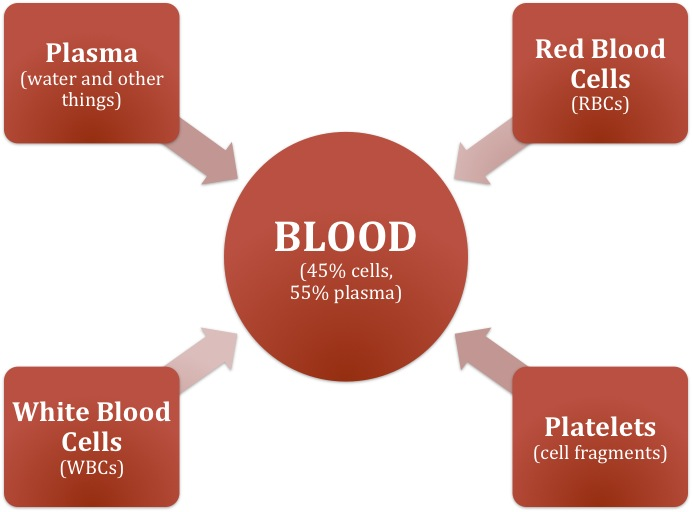
\includegraphics[width=0.7\textwidth]{basic_blood_diagram.jpg}
	    \caption{Συστατικά του αίματος}
	    \label{fig:basic_blood_diagram}
	\end{figure}
	 
	Το πλάσμα αποτελεί το μεγαλύτερο και κύριο συστατικό του αίματος, καταλαμβάνοντας το 55\% του συνολικού όγκου του. Είναι ένα υποκίτρινο υγρό μέσω του οποίου μεταφέρονται αιμοσφαίρια, πρωτεΐνες και άλλες ουσίες. Αποτελείται κατά 91,5\% από νερό, κατά 7\% από πρωτεΐνες, όπως η λευκωματίνη (αλβουμίνη), οι σφαιρίνες και το ινωδογόνο, και κατά 1,5\% από άλλες ουσίες, όπως θρεπτικά συστατικά, ορμόνες, αναπνευστικά αέρια, ηλεκτρολύτες, βιταμίνες και άχρηστες αζωτούχες ουσίες \cite{bloodPlasma}. Η κύρια λειτουργία που επιτελεί είναι η μεταφορά υγρών και υδατοδιάλυτων ουσιών όπως είναι οι ορμόνες και βασικές .

	Το υπόλοιπο 45\% του αίματος αποτελείται από αιμοσφαίρια και κυρίως ερυθρά αιμοσφαίρια, λευκά αιμοσφαίρια και αιμοπετάλια. Τα ερυθρά αιμοσφαίρια είναι τα πιο πολυάριθμα κύτταρα σε κυκλοφορία και δίνουν στο αίμα το χαρακτηριστικό κόκκινο χρώμα του. Τα ερυθρά αιμοσφαίρια χρησιμοποιούνται ευρέως, για να αναπληρώνουν την απώλεια αίματος που προκαλείται από αιμορραγία κατά τη γέννα, κατά τη διάρκεια χειρουργικής επέμβασης και κατά τη διάρκεια ατυχημάτων. Η μετάγγιση ερυθρών αιμοσφαιρίων μπορεί επίσης να είναι σωτήρια για τη ζωή του ασθενούς σε συγκεκριμένους τύπους αναιμίας. Η λειτουργία τους αφορά τη διατήρηση των ιστών στη ζωή καθώς μεταφέρουν σε αυτούς οξυγόνο και απομακρύνουν το διοξείδιο του άνθρακα. Η εκατοστιαία αναλογία ερυθρών αιμοσφαιρίων ανά μονάδα όγκου αίματος ονομάζεται αιματοκρίτης \cite{hematologyBasics}.
	
	Τα λευκά αιμοσφαίρια ή λευκοκύτταρα (WBC) αποτελούν λιγότερο από το 1\% του ολικού αίματος. Η πρωταρχική λειτουργία των λευκοκυττάρων είναι η καταπολέμηση των λοιμώξεων μέσω της επίθεσης και της καταστροφής επιβλαβών ξένων ουσιών. Σχηματίζονται στο μυελό των οστών, στη σπλήνα και τους λεμφαδένες \cite{whiteBloodCells}.
	
	Τα αιμοπετάλια ή θρομβοκύτταρα παράγονται από το μυελό των οστών και αποτελούν λιγότερο από το 1\% του πλήρους αίματος. Παίζουν καθοριστικό ρόλο στην πήξη του αίματος και την αιμόσταση, δηλαδή στην αναστολή της αιμορραγίας ή της κυκλοφορίας. Σχηματίζουν θρόμβους ώστε να αποτρέπεται η διαρροή αίματος από τις πληγές και αν ο αριθμός τους είναι χαμηλός, αυτό μπορεί να οδηγήσει σε εύκολη δημιουργία μωλώπων και σε μεγάλη αιμορραγία. Οι ασθενείς που έχουν λευχαιμία ή ανεπάρκεια μυελού των οστών, συνήθως έχουν χαμηλό ποσοστό αιμοπεταλίων και χρειάζονται αιμοπετάλια, για να διαφυλάξουν τη λειτουργία της πήξης του αίματός τους \cite{hematologyBasics}.
	
	Στο σχήμα \ref{fig:blood_cells_characteristics} βλέπουμε μια σύνοψη των βασικών χαρακτηριστικών των συστατικών του αίματος.
\begin{figure}[H]
	    \centering
	    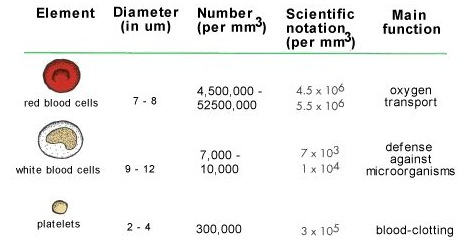
\includegraphics[width=0.7\textwidth]{blood_cells_characteristics.jpg}
	    \caption{Χαρακτηριστικά των κυττάρων του αίματος}
	    \label{fig:blood_cells_characteristics}
\end{figure}

	Τα κύτταρα του αίματος ανανεώνονται συνεχώς, όπως φαίνεται από τη διάρκεια ζωής στο αίμα των ερυθρών αιμοσφαιρίων (120 ημέρες), των αιμοπεταλίων (10 ημέρες) και των κοκκιοκυττάρων (9 ώρες). Ο χρόνος ζωής των λεμφοκυττάρων (Τ και Β κυττάρων) ποικίλλει εξαιρετικά από ώρες έως χρόνια. Η παραγωγή ενεργών κυττάρων του αίματος λαμβάνει χώρα κατά κύριο λόγο στο μυελό των οστών. Ωστόσο ο σπλήνας, οι λεμφαδένες και οι βοηθητικοί λεμφοειδείς ιστοί είναι επίσης θέσεις συνεχιζόμενης παραγωγής κυττάρων, κυρίως λεμφικής σειράς \cite{textbookOfMedicine}.
	
	Ένας υγιής ενήλικας έχει περίπου 5-6 λίτρα αίματος \cite{bloodVolume}, και μπορεί να υποστεί απώλεια 500 ml χωρίς να υποστεί προβλήματα υγείας και να χρειαστεί κάποια μετάγγιση αίματος. Βέβαια άμα υποστεί απώλεια της τάξης των 1000-1500 ml σε μικρό χρονικό διάστημα ή κάποια συστατικά του αίματος (αιμοπετάλια, ερυθρά αιμοσφαίρια) είναι κάτω από τα απαιτούμενα επίπεδα λόγω ασθένειας (καρκίνος, αναιμία κτλπ) ή λόγω κάποιας εγχείρησης, τότε χρειάζεται μετάγγιση αίματος \cite{Stainsby01092000}.
		\subsubsection{Ομάδες αίματος και συμβατότητα}	
			Στην επιφάνεια του ερυθρού αιμοσφαιρίου υπάρχουν διάφορα αντιγόνα ή ουσίες των ομάδων αίματος (blood group substances). Σήμερα είναι γνωστά 23 συστήματα ομάδων αίματος, γενετικά ανεξάρτητα το ένα από το άλλο. Κληρονομούνται σύμφωνα με τους νόμους του Mendel και η γνώση τους είναι εξαιρετικά χρήσιμη στην Ιατροδικαστική (έλεγχος πατρότητας), σε ανθρωπολογικές μελέτες αλλά κυρίως για τη σωστή και ασφαλή μετάγγιση αίματος στην κλινική πράξη \cite{dawkins}. Κάθε σύστημα ομάδων αίματος περιλαμβάνει μία σειρά αντιγόνων που σχετίζονται ως προς τη δομή. Συνολικά, τα συστήματα αυτά περιλαμβάνουν περισσότερα από 400 αντιγόνα. Οι ουσίες των ομάδων αίματος δεν περιορίζονται μόνο στη μεμβράνη των ερυθρών αιμοσφαιρίων αλλά βρίσκονται ακόμη σε κύτταρα πολλών ιστών καθώς και σε υγρά του σώματος, όπως σάλιο, γαστρικό υγρό, σπέρμα, ούρα, και γάλα. Τα συστήματα ομάδας αίματος συμπεριλαμβάνουν τα ΑΒΟ, τα Rh, MNS, Kell, Duffy, Kidd και άλλα.
			
			Το πιο γνωστό και πιο ευρείας χρήσης είναι το σύστημα ΑΒΟ. Είναι το πρώτο σύστημα που ανακαλύφθηκε το 1900 από τον Landsteiner (Βραβείο Νομπέλ Ιατρικής 1930) \cite{landsteinerABO}. Η ανακάλυψη αυτή άνοιξε το δρόμο για την ασφαλή μετάγγιση αίματος. Το σύστημα ΑΒΟ εξακολουθεί και σήμερα να είναι το πιο σημαντικό στη μετάγγιση. Το σύστημα συνδέεται με τρία αντιγόνα Α, Β και Η. Το σύστημα χαρακτηρίζεται από την παρουσία ή την απουσία στα ερυθρά αιμοσφαίρια των αντιγόνων (συγκολλητινογόνων). Με συνδυασμό αυτών διακρίνονται τέσσερις ομάδες αίματος, η ΑΒ, η Α, η Β, και η Ο. Η ομάδα ΑΒ χαρακτηρίζεται από την παρουσία στα ερυθρά αιμοσφαίρια και των δύο αντιγόνων Α και Β. Η ομάδα Α χαρακτηρίζεται από την παρουσία του αντιγόνου Α. Η ομάδα Β χαρακτηρίζεται από την παρουσία του αντιγόνου Β. Τέλος η ομάδα Ο δεν περιέχει κανένα από τα αντιγόνα Α ή Β, αλλά περιέχει το αντιγόνο Η. Το τελευταίο υπάρχει σε όλες τις ομάδες αλλά ιδιαιτέρως παρατηρείται στην ομάδα Ο.
			
			Στον ορό του αίματος των διαφόρων ατόμων παρατηρούνται φυσιολογικές συγκολλητίνες ομόλογοι των συγκολλητινογόνων Α και Β. Οι φυσιολογικές συγκολλητίνες είναι οι α (anti- A) και οι β (anti-B). Στον ορό δεν υπάρχει ποτέ η συγκολλητίνη η ομόλογος προς το συγκολλητινογόνο που υπάρχει στα ερυθρά αιμοσφαίρια του ιδίου ατόμου. Έτσι στον ορό του αίματος ΑΒ δεν υπάρχει καμία συγκολλητίνη. Στον ορό της ομάδας Α υπάρχει η συγκολλητίνη anti-B ή β. Στον ορό της ομάδας Β υπάρχει η συγκολλητίνη anti-Α ή α. Τέλος στον ορό της ομάδας Ο υπάρχουν και οι δύο συγκολλητίνες α και β. Η συγκολλητίνη α αντιδρά με το συγκολλητινιγόνο Α και η συγκολλητίνη β αντιδρά με το συγκολλητινιγόνο Β. Εάν επομένως σε μία μετάγγιση αίματος ο ορός του ασθενούς (δέκτη) έχει συγκολλητίνες (α ή β, α και β), τότε αυτές θα συγκολλήσουν τα ερυθρά αιμοσφαίρια του δότη, όταν στα αιμοσφαίρια αυτά υπάρχουν συγκολλητινογόνα Α ή Β ή Α και Β. Στην περίπτωση αυτή τα συγκολλημένα ερυθρά αιμοσφαίρια μπορεί να προκαλέσουν ακόμη και το θάνατο του δέκτη. Στο σχήμα \ref{fig:blood_antibodies_antigons} φαίνονται συγκεντρωτικά τα στοιχεία που αναλύσαμε παραπάνω.		
	\begin{figure}[h!]
	    \centering
	    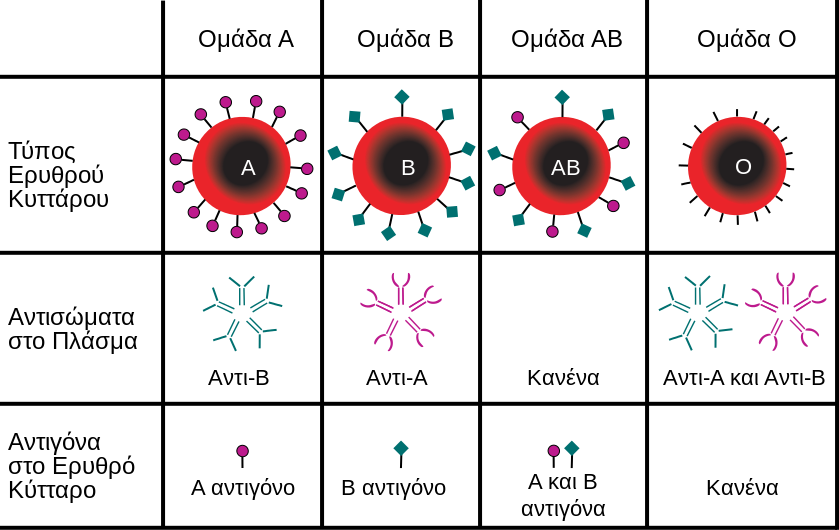
\includegraphics[width=0.7\textwidth]{blood_antibodies_antigons.png}
	    \caption{Αντισώματα και αντιγόνα του αίματος}
	    \label{fig:blood_antibodies_antigons}
	\end{figure}
			
			Στις μεταγγίσεις πρέπει να λαμβάνεται υπόψη και ένας άλλος
παράγοντας, που λέγεται παράγοντας Rhesus, επειδή ανακαλύφθηκε πρώτα στα ερυθρά
αιμοσφαίρια του πιθήκου Rhesus Maccacus. Το σύστημα Rhesus είναι το δεύτερο κατά
σπουδαιότητα σύστημα ομάδων αίματος μετά το ΑΒΟ. Η γνώση του είναι απαραίτητη για
την ασφαλή μετάγγιση αίματος, ενώ είναι το σύστημα, που κυρίως ευθύνεται για την
αιμολυτική νόσο του νεογνού. Σήμερα είναι γνωστά περί τα 50 αντιγόνα που ανήκουν στο
σύστημα Rhesus. Από αυτά τα πέντε είναι τα κύρια και βασικά. Το κυριότερο αντιγόνο είναι
το D και άτομα που το έχουν στα ερυθρά αιμοσφαίρια είναι Rh-Θετικά ή Rh (+), ενώ αυτά
που δεν το έχουν είναι Rh-Αρνητικά ή Rh (-). Το αντιγόνο D είναι εξαιρετικά ανοσογόνο
(immunogenic) και άτομα Rh-Αρνητικά, όταν εκτεθούν σε αυτό, μπορούν να σχηματίσουν
anti-D αντισώματα. Το 85\% των λευκών ανθρώπων έχουν τον παράγοντα αυτό, δηλαδή είναι
Rh-Θετικοί και το 15\% δεν το έχουν, δηλαδή είναι Rh-Αρνητικοί \cite{Landsteiner01011940}. 

Συμβάντα μπορεί να παρατηρηθούν, αν δεν προσδιοριστεί ο παράγοντας Rhesus, στις εξής
περιπτώσεις.
\begin{enumerate}
	\item Σε άτομα στα οποία έγινε μια πρώτη μετάγγιση και στα οποία μια δεύτερη μετάγγιση μπορεί να είναι θανατηφόρα
	\item Στις γυναίκες στις οποίες γίνεται μετάγγιση κατά τη διάρκεια της εγκυμοσύνης τους
	\item Στις γυναίκες που γέννησαν ήδη το πρώτο τους παιδί και στις οποίες μετά από λίγο γίνεται μετάγγιση
	\item Στα έμβρυα λόγω του παράγοντα Ρέζους μπορεί να προκληθεί μια πολύ σοβαρή πάθηση που λέγεται ερυθροβλάστωση των εμβρύων (αν η μητέρα είναι Ρέζους αρνητική, ο πατέρας Ρέζους θετικός και το έμβρυο επίσης Ρέζους θετικό). Κατά την αρρώστια αυτή τα αιμοσφαίρια του εμβρύου συγκολλούνται και προκαλείται τελικά ο θάνατος του. Μπορεί να σωθεί μόνο, αν γεννηθεί ζωντανό και γίνει αλλαγή του αίματος του (αφαιμαξομετάγγιση) με άλλο αίμα Ρέζους αρνητικό
\end{enumerate}

Βάση όσων έχουν αναφερθεί παραπάνω, στο σχήμα \ref{fig:blood_compatibility} βλέπουμε την συμβατότητα των διάφορων συνδυασμών.
	\begin{figure}[h!]
	    \centering
	    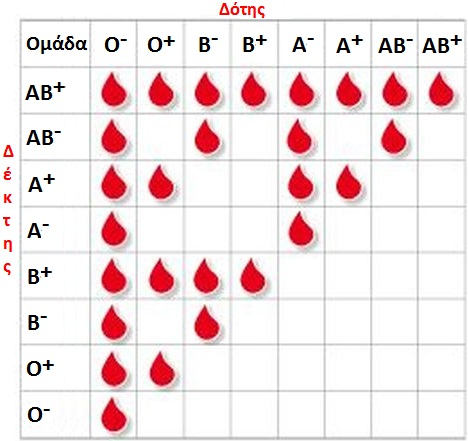
\includegraphics[width=0.5\textwidth]{blood_compatibility.jpg}
	    \caption{Συμβατότητα ομάδων αίματος}
	    \label{fig:blood_compatibility}
	\end{figure}
	
	Από την άλλη μεριά η μετάγγιση πλάσματος έχει τους αντίθετους κανόνες αφού τα αντιγόνα βρίσκονται στο πλάσμα. Για παράδειγμα ένας ασθενής με τύπο αίματος O μπορεί να λάβει πλάσμα από τις ομάδες αίματος A,B και ΑΒ αφού το πλάσμα του τύπου Ο περιέχει αντιγόνα και της Α και της Β. Στον πίνακα \ref{tab:plasma_compatibility} βλέπουμε τη συμβατότητα πλάσματος των διάφορων συνδυασμών.
\begin{table}[H]
	\centering
	\begin{tabular}{l|llll}
		Ασθενής & \multicolumn{4}{l}{Αιμοδότης} \\ \hline
			& Ο     & Α     & Β     & ΑΒ    \\
		Ο       & Ναι   & Ναι   & Ναι   & Ναι   \\
		Α       & Όχι   & Ναι   & Όχι   & Ναι   \\ 
		Β       & Όχι   & Όχι   & Ναι   & Ναι   \\
		ΑΒ      & Όχι   & Όχι   & Όχι   & Ναι  
	\end{tabular}
	\caption{Συμβατότητα πλάσματος}
	\label{tab:plasma_compatibility}
\end{table}
	Σε αυτό το σημείο θα πρέπει να αναφερθεί ότι η κατανομή του πληθυσμού στις διάφορες ομάδες αίματος δεν είναι ισόποση. Στο σχήμα \ref{fig:blood_distribution} βλέπουμε την κατανομή σε επιλεγμένες χώρες.
\begin{figure}[h!]
	    \centering
	    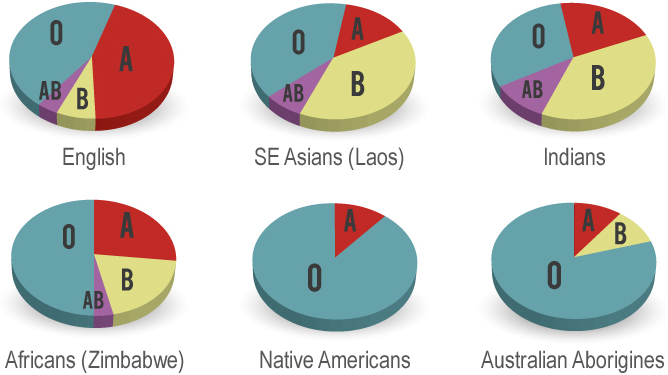
\includegraphics[width=0.7\textwidth]{blood_distribution.jpg}
	    \caption{Κατανομή ομάδων αίματος}
	    \label{fig:blood_distribution}
\end{figure}	

	\subsection{Αιμοδοσία}
	Με τον όρο αιμοδοσία εννοούμε τη χορήγηση αίματος από υγιείς δότες σε άτομα στα
οποία η κατάσταση της υγείας τους απαιτεί μετάγγιση. Κατ' επέκταση με τον όρο αιμοδοσία εννοούμε την όλη οργάνωση που ασχολείται με τη λήψη, επεξεργασία, συντήρηση και διάθεση του αίματος και των Παραγώγων του \cite{bloodDonationDefinition}. Η αιμοδοσία καλείται εθελοντική, επειδή αφορά σε πράξη που εκτελεί κάποιος με τη θέλησή του και με μοναδικά κίνητρα αισθήματα αλληλεγγύης και αλτρουισμού \cite{1973}. 

Ως επιστημονικός τομέας, η αιμοδοσία αποτελεί ιδιαίτερο κλάδο της αιματολογίας με τεράστια ανάπτυξη τα τελευταία 20 χρόνια. Η ανάπτυξη της αιμοδοσίας ως εξειδικευμένου τομέα, καθώς και η αλματώδης ανάπτυξή της, οδήγησαν στην ανάγκη να πλαισιώνεται από ιατρικό, νοσηλευτικό και τεχνικό προσωπικό υψηλής στάθμης με εξειδίκευση στον τομέα της
αιμοδοσίας.  
	
	Η μετάγγιση αίματος γίνεται τακτικά σε εγχειρήσεις, τραυματίες, γαστρορραγίες και σε τοκετούς για την αναπλήρωση της απώλειας σημαντικής ποσότητας αίματος. Στις περισσότερες περιπτώσεις η μετάγγιση αίματος χρησιμοποιείται ως προσωρινή μορφή θεραπείας. Σε αυτές τις περιπτώσεις ο ασθενής χρειάζεται αρκετές μονάδες αίματος αλλά μόλις η κατάσταση του θεωρηθεί εκτός κινδύνου, δεν χρειάζεται περεταίρω μετάγγιση αίματος. Βέβαια, υπάρχουν και περιπτώσεις όπου ο ασθενής χρειάζεται μεταγγίσεις αίματος εφόρου ζωής. Μερικές ευρέως γνωστές ασθένειες που απαιτούν κάτι τέτοιο είναι η Β-Θαλασσαιμία (η Ελλάδα έχει τα υψηλότερα ποσοστά), αιμοφιλία και λευχαιμία \cite{thalassaemiaLongTerm}.

	Αν και υπάρχουν κάποιες περιπτώσεις οι οποίες απαιτούν μετάγγιση ολικού αίματος, η πλειονότητα του αίματος διασπάται μετά την δωρεά και τα απαιτούμενα προϊόντα αίματος μεταφέρονται στον ασθενή. Ακολουθώντας την παραπάνω προσέγγιση, από την μία μεριά ο ασθενής δεν λαμβάνει περιττά συστατικά και από την άλλη μεριά από μία μονάδα ολικού αίματος μπορούν να επωφεληθούν περισσότερα του ενός ατόμου. Η διάρκεια ζωής των διάφορων συστατικών του αίματος φαίνονται στον πίνακα \ref{tab:blood-shelf-life} παρακάτω \cite{Basu2014}:
	
\begin{table}[H]
		\centering
		\begin{tabular}{l|ll}
			\hline
			Συστατικό          & Διάρκεια  & Θερμοκρασία \\ \hline
			Ολικό αίμα         & 24 ώρες   & 20-24       \\
			Ερυθρά αιμσοφαίρια & 42 μέρες  & 4           \\
			Αιμοπετάλια        & 3-5 μέρες & 20-24       \\
			Πλάσμα             & 1 χρόνος  & -18        
		\end{tabular}
		\caption{Διάρκεια ζωής συστατικών αίματος}
		\label{tab:blood-shelf-life}
\end{table}	

Από τα δεδομένα του παραπάνω πίνακα γίνεται εύκολα εμφανές ότι είναι προτιμότερο να αποθηκευόνται τα συστατικά του αίματος πάρα το ολικό αίμα, ενώ παράλληλα γίνεται εμφανής η ανάγκη για συνεχή παροχή αιμοδοσιών.
	
	 Το αίμα που χρησιμοποιείται στις μεταγγίσεις πρέπει να προέρχεται από υγιή άτομα. Το αίμα δεν είναι μόνο ζωντανός ιστός, αλλά έχει επιπλέον την ιδιότητα να ανανεώνεται και τα υγιή άτομα διαθέτουν μηχανισμούς αύξησης της παραγωγής αίματος. Έτσι με την αιμοδοσία προσφέρεται εύκολα το δώρο της ζωής χωρίς το φόβο ότι η τακτική αιμοδοσία θα προκαλέσει εξασθένηση του οργανισμού και θα οδηγήσει σε αδυναμία η επιτάχυνση της γήρανσης.
	 
	Στόχος είναι οι εθελοντές, που πληρούν τα κριτήρια για αιμοδοσία να γίνονται τακτικοί αιμοδότες, δηλαδή να πραγματοποιούν δωρεά αίματος αρκετές φορές το χρόνο και να παραμένουν στον κατάλογο των ενεργών αιμοδοτών για πολλά χρόνια. Η διατήρηση ενός υψηλού επιπέδου ποιότητας παρεχόμενων υπηρεσιών στην υπηρεσία αιμοδοσίας συνίσταται στην προτεραιότητα ικανοποίησης των αναγκών και των προσδοκιών των εθελοντών αιμοδοτών. Ωστόσο είναι σημαντικό να επισημάνουμε ότι μια επένδυση στην προσέλκυση και την διατήρηση εθελοντών, δεν θα αποδώσει μόνο ασφαλή αποθέματα αίματος και προστασία της υγείας τόσο στον δότη όσο και στον λήπτη, αλλά και σημαντική εξοικονόμηση κόστους για την υπηρεσία μέσω της μείωσης του αριθμού μονάδων αίματος που πρέπει να απορριφθούν λόγω της ανεύρεσης θετικών δεικτών λοιμωδών νοσημάτων. 
	
	Επιπλέον η προσέλκυση και η διατήρηση των εθελοντών αιμοδοτών είναι μια δυναμική λειτουργία που σχεδιάζεται κάθε φορά ανάλογα με την μελέτη και ανάλυση των παραμέτρων της συγκεκριμένης κοινωνικής ομάδας που απευθυνόμαστε σε σχέση με την αξιολόγηση και εκτίμηση των αναγκών σε αίμα και την υπάρχουσα κατάσταση στο χώρο της.
		\subsubsection{Διαδικασία της Αιμοδοσίας}
		 Η επιλογή των αιμοδοτών γίνεται από άρτια εκπαιδευμένο και επαγγελματικά καταρτισμένο προσωπικό που έχει ως σκοπό την ασφάλεια τόσο του αιμοδότη όσο και του δέκτη. Στην είσοδο της αιμοδοσίας υπάρχουν ειδικά έντυπα αυτοαποκλεισμού, τα οποία καλούνται να διαβάσουν όλοι οι άνθρωποι που προσέρχονται προκειμένου να προσφέρουν αίμα \cite{diadikasiaAimodosias}. Στην συνέχεια αν ο δυνητικός αιμοδότης κρίνει ότι πληροί τα κριτήρια αποδοχής και δεν ισχύει κάποιο από τα κριτήρια αποκλεισμού για την περίπτωση του, θα πρέπει να συμπληρώσει το ερωτηματολόγιο του αιμοδότη \cite{ekeaQuestionnaire} (περισσότερα στο Παράρτημα Α). Το προαναφερθέν ερωτηματολόγιο είναι εμπιστευτικό διασφαλίζοντας το ιατρικό απόρρητο και θα πρέπει να συμπληρώνεται από τον αιμοδότη κάθε φορά που θέλει να δώσει αίμα. Ο αιμοδότης έχει τη δυνατότητα να συζητήσει με τον ιατρό προβλήματα υγείας ή άλλους λόγους που θέτουν ενδεχομένως σε κίνδυνο την ασφάλεια του ίδιου ή του δέκτη.
		 
		 Στην συνέχεια ο αιμοδότης εξετάζεται για την αρτηριακή πίεση, σφυγμό, βάρος, αιματοκρίτη ή αιμοσφαιρίνη, πιθανές δερματικές αλλοιώσεις στο σημείο της φλεβοκέντησης καθώς και για τη φυσική του κατάσταση. Ο γιατρός της αιμοδοσίας, εφόσον συλλέξει τις απαραίτητες πληροφορίες και λαμβάνοντας υπόψιν τις απαντήσεις στο ερωτηματολόγιο του αιμοδότη, κρίνει αν μπορεί κάποιος, ο οποίος προσέρχεται στην υπηρεσία αιμοδοσίας, είναι σε θέση να προσφέρει αίμα. Η τελική ευθύνη για την επιλογή του αιμοδότη βαρύνει τον ιατρό της αιμοδοσίας.
		 
		Πρέπει να σημειωθεί, σε αυτό το σημείο, πως είναι απαραίτητη η έγγραφη συγκατάθεση του αιμοδότη ότι δέχεται να αιμοδοτήσει και να εξεταστεί το αίμα του για μεταδοτικά νοσήματα. Σε περίπτωση απόρριψης δίνονται οι απαραίτητες ιατρικές πληροφορίες και εξηγήσεις οι οποίες αφορούν στο λόγο και στη διάρκεια αποκλεισμού (για περισσότερα βλ: \ref{sssec:donor_screening}).
		
		Αφού κριθεί ότι ο αιμοδότης πληροί τις προϋποθέσεις, οδηγείται στην ειδική καρέκλα της αιμοδοσίας, γίνεται περίδεση του βραχίονα και καλή αντισηψία στην περιοχή της φλεβοκέντησης. Κατά τη διαδικασία της αιμοληψίας συστήνεται στον αιμοδότη να ανοιγοκλείνει τη γροθιά του, ώστε να διευκολύνεται η ροή του αίματος. Λαμβάνονται 450ml αίματος. Ο όγκος του αίματος, που προσφέρεται, αναπληρώνεται μέσα σε 24 ώρες μετά την αιμοδοσία.
		
		Μετά την αιμοληψία, το αίμα συλλέγεται σε ειδικούς σάκους, που περιέχουν αντιπηκτικές και άλλες ουσίες, οι οποίες βοηθούν στην άριστη διατήρηση του αίματος. Πριν αφαιρεθεί η βελόνα λαμβάνονται δείγματα για τις εξετάσεις, όπως προβλέπεται από το νόμο. Στο τέλος, ο αιμοδότης καλείται να παραμείνει καθιστός για λίγη ώρα, καθώς παράλληλα σε κάποια κέντρα του προσφέρεται χυμός και κάποιο μικρό πρόχειρο γεύμα.
		
		Πρόκειται για μια ανώδυνη διαδικασία. Μοναδικό ενόχλημα είναι ένας μικρός πόνος από τη βελόνα. Η αιμοδοσία είναι ακίνδυνη για τον αιμοδότη. Η περίπτωση να μολυνθεί ο αιμοδότης από AIDS ή άλλο μεταδιδόμενο νόσημα είναι μηδενική, αφού οι βελόνες που χρησιμοποιούνται είναι μιας χρήσης και αποστειρωμένες.
		
		Η αιμοδοσία διαρκεί περίπου δέκα λεπτά. Για την όλη διαδικασία, από τη συμπλήρωση του ερωτηματολογίου μέχρι να φύγει ο αιμοδότης, απαιτείται περίπου μισή ώρα \cite{diadikasiaAimodosias}.
	\subsection{Εθελοντές αιμοδότες}
		\subsubsection{Κριτήρια επιλογής αιμοδοτών} \label{sssec:donor_screening} 
			Αίμα μπορούν να δώσουν όλοι οι υγιείς άντρες και γυναίκες ηλικίας 18 - 65 ετών οι οποίοι έχουν σωματικό βάρος μεγαλύτερο των 50 κιλών, κάθε 3 - 4 μήνες. Βασικός στόχος και υποχρέωση των υπηρεσιών μετάγγισης αίματος είναι να συλλέξουν αίμα από υγιείς αιμοδότες, ώστε αφενός να προφυλαχθεί η δική τους υγεία και αφετέρου να προστατευθεί ο αιμολήπτης ασθενής από τη μετάδοση ασθενειών ή φαρμακευτικών ουσιών που μπορεί δυνητικά να είναι βλαβερά για την υγεία του. Ο υποψήφιος αιμοδότης κατά τη λήψη του ιστορικού πρέπει να αναφέρει τυχόν συμπτώματα, ώστε να βοηθήσει το ιατρικό προσωπικό να κρίνει με ασφάλεια την πιθανότητα κινδύνου. Κάθε πρόβλημα υγείας που ενδεχομένως έχει ο υποψήφιος αιμοδότης, πρέπει να συζητείται με τον υπεύθυνο γιατρό της αιμοδοσίας, ο οποίος και κρίνει τελικά για τη καταλληλότητα της αιμοληψίας. Η διαδικασία θα πρέπει να είναι τέτοια έτσι ώστε και να εξασφαλίζεται ασφαλή αιμοδοσία και παροχή αίματος αλλά και να μην απορρίπτονται υγιείς αιμοδότες οι οποίοι θα μπορούσαν να συνεισφέρουν \cite{bloodDonorSelection}.
			
			Ο αιμοδότης πρέπει να είναι σε καλή υγεία και απαλλαγμένος από μεταδοτικές ασθένειες. Όμως κάθε άνθρωπος είναι επιρρεπής σε μικρο-αδιαθεσίες. Αυτές είναι πόνοι κάθε είδους, ακμή, πονόλαιμοι και δυσπεψία. Όλα αυτά δεν αποτελούν στοιχεία απόρριψης του αιμοδότη. Εάν ο δότης υποβάλλεται σε φαρμακευτική αγωγή ή έχει υποβληθεί στο άμεσο παρελθόν, πρέπει να σημειωθούν τα παρακάτω σχετικά με τα φάρμακα που παίρνει. Η ποσότητα του φαρμάκου, δηλαδή η πυκνότητα του φαρμάκου στον οργανισμό του δότη και η ταχύτητα απορρόφησης ή η αποβολή του. Το φάρμακο μπορεί να έχει δυσμενή επίπτωση στο δέκτη εφόσον η περιεκτικότητα του φαρμάκου στο δότη είναι αυξημένη. Εάν ο δέκτης είναι αλλεργικός σ' αυτό το φάρμακο ή εάν ο δέκτης είναι έγκυος γυναίκα μπορεί να προκληθεί μέχρι και τερατογένεση. Το φάρμακο μπορεί να διαταράξει το αίμα του δότη, π.χ. τη λειτουργικότητα των αιμοπεταλίων. Παρόλο ότι τα φαινόμενα αυτά έχουν αναγνωριστεί, η συχνότητά τους δεν μελετήθηκε ακόμη καλά. Εάν λοιπόν ο αιμοδότης λαμβάνει φάρμακα, δεν σημαίνει ότι αναγκαστικά δεν μπορεί να προσφέρει αίμα. Σε κάθε περίπτωση όμως είναι ορθό να ενημερώνεται ο γιατρός και το προσωπικό για τα φάρμακα που λαμβάνει και ανάλογα θα κριθεί εάν μπορεί να προσφέρει αίμα \cite{bloodDonorSelection}. 
			
		Υπάρχουν καταστάσεις και νοσήματα που αποκλείουν δια παντός την αιμοδοσία, όπως είναι το AIDS, οι ηπατίτιδες, η ελονοσία, η χρήση ενδοφλεβίων ναρκωτικών, οι κακοήθειες, η υπέρταση, ο σακχαρώδης διαβήτης ή σοβαρά χρόνια νοσήματα. Στις περισσότερες περιπτώσεις, όμως, ο αποκλεισμός είναι μόνο πρόσκαιρος.  Ο αποκλεισμός αυτός γίνεται για να μην επιβαρυνθεί η υγεία του αιμοδότη και για να διασφαλιστεί η ποιότητα του αίματος που θα μεταγγιστεί στο λήπτη. Μελέτες έχουν δείξει ότι ο προσωρινός αποκλεισμός από την αιμοδοσία έχει έντονο αρνητικό αντίκτυπο στην μελλοντική επιστροφή του αιμοδότη \cite{Custer2011}\cite{Custer2007}. Για αυτό είναι υψίστης σημασίας να δίνονται ξεκάθαρα διαστήματα αποκλεισμού και να ενθαρρύνονται οι εθελοντές να επιστρέψουν μετά το πέρας αυτού του διαστήματος. Στο σύστημα που προτείνουμε στη παρόν διπλωματική έχει γίνει μέριμνα για τέτοιες περιπτώσεις και προτείνετε ένα σύστημα κατάλληλων ειδοποιήσεων.
		
		Εκτός από τις γενικές αυτές αρχές και επειδή οι λεπτομέρειες στις ενδείξεις αναπροσαρμόζονται, ο υποψήφιος αιμοδότης πρέπει να συμβουλεύεται το προσωπικό της αιμοδοσίας που είναι το πλέον αρμόδιο για την επιλογή των αιμοδοτών.
		\subsubsection{Κατηγορίες αιμοδοτών}
			Οι αιμοδότες μπορούν να χωριστούν σε τρεις μεγάλες κατηγορίες:
\begin{enumerate}
	\item Οι εθελοντές αιμοδότες (Volunteer Donors - VDs) οι οποίοι αιμοδοτούν με δική τους πρωτοβουλία καθαρά για ανθρωπιστικούς λόγους, χωρίς να λαμβάνουν κάποιο οικονομικό αντάλλαγμα ή οτιδήποτε που θα μπορούσε να θεωρηθεί ως αντικαταστατό του χρήματος.
	\item Οι δότες αντικατάστασης (Replacement Donors - RDs), οι οποίοι αιμοδοτούν προκειμένου να καλύψουν τις ανάγκες που προκύπτουν από συγγενείς ή φίλους οι οποίοι νοσηλεύονται.
	\item Δότες αίματος επί πληρωμή οι οποίοι λαμβάνουν πληρωμή από την οικογένεια η οποία δεν μπορεί να παρέχει η ιδία δότη αντικατάστασης για το συγγενικό τους πρόσωπο.
\end{enumerate} 

		Σε αυτό το σημείο ότι η τρίτη κατηγορία αιμοδοτών εμφανίζεται μόνο σε τριτοκοσμικές χώρες και κυρίως σε χώρες της Αφρικής. Στατιστικά στοιχεία έχουν δείξει ότι οι τακτικοί εθελοντές αιμοδότες (VDs) σχετίζονται με ασφαλέστερες παροχές αίματος σε σχέση με τους δότες αντικατάστασης όσον αφορά τις μεταδιδόμενες κατά την μετάγγιση ασθένειες \cite{Liu1998}.

		Στοιχεία του Παγκόσμιου Οργανισμού Υγείας (WHO) και του Συμβουλίου της Ευρώπης υποδεικνύουν ότι το αίμα και τα παράγωγα του αίματος θα πρέπει να συλλέγονται αποκλειστικά από τακτικούς μη αμειβόμενους εθελοντές \cite{VOX:VOX5295}. Τα συστήματα αιμοδοσίας τα οποία στηρίζονται στους εθελοντές αιμοδότες οι οποίοι δίνουν αίμα σε σταθερή βάση, έχουν τη δυνατότητα να διαχειριστούν καλύτερα τις παροχές αίματος και να προγραμματίσουν τις μεταγγίσεις, επιταχύνοντας την όλη διαδικασία. Τέλος, από ηθική άποψη, δεν είναι σωστό να αναγκάζονται οι συγγενείς ενός ασθενούς σε ανάγκη, να αναζητούν κάτω από ψυχολογική πίεση άτομα για να προσφέρουν αίμα προκειμένου να καλυφθούν οι ανάγκες του δικού τους ανθρώπου.

		Οι εθελοντές αιμοδότες (VDs) μπορούν να χωριστούν περεταίρω στις ακόλουθες κατηγορίες \cite{karabaggeli-blatsa}:
		\begin{enumerate}
			\item Στους συστηματικούς και αυτόνομους, οι οποίοι προσέρχονται να αιμοδοτήσουν με δική τους αποκλειστικά πρωτοβουλία.
			\item Στους οργανωμένους σε συλλόγους ή τράπεζες αίματος που καλούνται να δώσουν αίμα.
			\item Στους περιστασιακούς που απαντούν σε εκκλήσεις ραδιοφωνικών σταθμών και άλλων μέσων.
			\item Στους εποχιακούς που δίνουν αίμα κατά την ημέρα της αιμοδοσίας του Δήμου, του πολιτιστικού συλλόγου που ανήκουν και άλλων οργανώσεων.
		\end{enumerate}
		
		Ο πραγματικός βέβαια εθελοντής αιμοδότης είναι εκείνος που προσέρχεται να δώσει αίμα με μοναδικό κίνητρο την κοινωνική αλληλεγγύη και τον αλτρουισμό, δεν τον απασχολεί σε ποιον θα δοθεί το αίμα που πρόσφερε και δεν περιμένει κανένα απολύτως αντάλλαγμα.
				
	\subsection{Εθελοντική αιμοδοσία στην Ελλάδα}
		Στην Ελλάδα το "Εθνικό Κέντρο Αιμοδοσίας" (Ε.ΚΕ.Α) το οποίο στεγάζεται στο Υπουργείο Υγείας και Πρόνοιας αποτελεί το κεντρικό όργανο για την οργάνωση των Υπηρεσιών Αιμοδοσίας. Οι Υπηρεσίες Αιμοδοσίας μπορούν να διαχωριστούν στις παρακάτω τρεις κατηγορίες:
		\begin{enumerate}
			\item Κέντρα Αίματος
			\item Σταθμοί Αιμοδοσίας Α' Τάξης
			\item Σταθμοί Αιμοδοσίας Β' Τάξης
		\end{enumerate}
				 
		 Τα κέντρα Αίματος καλύπτουν τις ανάγκες μιας ευρύτερης γεωγραφικής περιοχής ή μεγάλων πληθυσμιακών ομάδων και εδρεύουν σε νοσοκομεία. Κάθε κέντρο αίματος εκτελεί μοριακούς έλεγχους για τους σταθμούς αιμοδοσίας της περιοχής του (για περισσότερα βλ. παράρτημα \ref{ch:blood_centers}) Η Ελλάδα διαθέτει 4 μεγάλα κέντρα αίματος: 
		\begin{enumerate}
			\item Ε.ΚΕ.Α - Εθνικό κέντρο αιμοδοσίας.
			\item Πανεπιστημιακό Νοσοκομείο ΑΧΕΠΑ Θεσσαλονίκης.
			\item Πανεπιστημιακό Νοσοκομείο Ρίο Πατρών.
			\item Πανεπιστημιακό Νοσοκομείο Βενιζέλειο Ηρακλείου Κρήτης.
		\end{enumerate}				 
		 
		 Οι σταθμοί Αιμοδοσίας Α' Τάξης είναι μικρότερες υπηρεσίες και καλύπτουν τις ανάγκες του νοσοκομείου στο οποίο εδρεύουν και άλλες τοπικές ανάγκες. Οι Σταθμοί Αιμοδοσίας Β' Τάξης καλύπτουν αποκλειστικά τις ανάγκες του νοσοκομείου που στεγάζονται.
		
		Το σύστημα αιμοδοσίας στην Ελλάδα είναι αποκεντρωμένο και αποτελείται από 101 υπηρεσίες αιμοδοσίας υπό την αιγίδα και εποπτεία του Υπουργείου Υγείας\cite{filloKivernisews}. Κάθε υπηρεσία αιμοδοσίας αποτελεί ένα ενσωματωμένο μέρος ενός δημόσιου νοσοκομείου και οι αρμοδιότητές της περιλαμβάνουν α) τη στρατολόγηση νέων αιμοδοτών, β) τη συλλογή και τον έλεγχο του αίματος και γ) και τη διακίνηση του αίματος και των παραγώγων του στις νοσοκομειακές κλινικές \cite{Marantidou2007}.
		
		Σύμφωνα με επίσημα δεδομένου του Υπουργείου Υγείας οι ανάγκες για αίμα το έτος 2014 στην Ελλάδα ήταν 750.000 μονάδες. Ένα σημαντικός παράγοντας ο οποίος αυξάνει σημαντικά τις ανάγκες σε αίμα στην χώρα μας και δικαιολογεί το παραπάνω νούμερο, είναι τα υψηλά ποσοστά μεσογειακής αναιμίας για τα οποία χρειάζονται 144.000 μονάδες αίματος ανά χρόνο. 
		
		Σύμφωνα με στοιχεία που έδωσε στη δημοσιότητα το Εθνικό Κέντρο Αιμοδοσίας (Ε.ΚΕ.Α) κατά την διάρκεια του έτους 2013 έγινε εθελοντική αιμοδοσία 584.088 μονάδων αίματος, εκ των οποίων 254.198 (43.52 \%) προήλθε από τους επονομαζόμενους δότες αντικατάστασης (Replacement Donors - RDs),οι οποίοι αιμοδοτούν προκειμένου να καλύψουν τις ανάγκες που προκύπτουν από συγγενείς ή φίλους. Ένα ποσοστό 54.85 \% δηλαδή 320.411 μονάδες προέρχονται από εθελοντές αιμοδότες (Volunteer Donors - VDs), οι οποίοι αιμοδοτούν με δική τους πρωτοβουλία καθαρά για ανθρωπιστικούς λόγους. Οι υπόλοιπες 9.479 μονάδες (0.016\%) προέρχονται από τις ένοπλες δυνάμεις. Η τελευταία αυτή κατηγορία αιμοδοτών έχει δυνατά κίνητρα να αιμοδοτήσει εθελοντικά, καθώς αποζημιώνονται με άδειες και αποχή από τα καθήκοντά τους. Σε αυτό το σημείο κρίνεται σκόπιμο να αναφερθεί ότι τα τελευταία τρία χρόνια έχει παρατηρηθεί αύξηση στις εθελοντικές αιμοδοσίες. Συγκεκριμένα το 2013 παρασχεθήκανε από εθελοντές αιμοδότες (VDs) 21.234 περισσότερες μονάδες αίματος σε σύγκριση με το 2012 \cite{EKEA}. Παρότι τα παραπάνω νούμερα είναι ενθαρρυντικά και παρότι διακρίνεται μια αυξητική τάση των εθελοντικών αιμοδοσιών, αξίζει να σημειωθεί ότι 24.000 μονάδες αίματος εισήχθησαν από την Ελβετία, προκειμένου να καλυφθούν οι εθνικές ανάγκες για αίμα \cite{Marantidou2007}.
		
		Βάση επίσημων στοιχείων, η Ελλάδα διαθέτει έναν ευρύ κατάλογο αιμοδοτών βάσει του οποίου 6 αιμοδότες αντιστοιχούν σε 100 πολίτες, γεγονός που την κατατάσσει τρίτη ανάμεσα στις χώρες- μέλη της Ευρωπαϊκής Ένωσης όσον αφορά τον αριθμό των ατόμων οι οποίοι έχουν δωρίσει αίμα έστω και μία φορά στη ζωή τους  (Eurobarometer, 2009).  Επίσης, η Ελλάδα έρχεται πρώτη όσον αφορά τους μη αιμοδότες, οι οποίοι όμως έχουν σκεφτεί να δώσουν αίμα (Eurobarometer, 2005). Παρόλα τα στοιχεία αυτά όμως, η Ελλάδα που είναι μία χώρα 11.000.000 κατοίκων, πολύ συχνά βρίσκεται στη δυσάρεστη αλλά αναπόφευκτη θέση να εισάγει αίμα από το εξωτερικό, καθώς ο ετήσιος αριθμός μονάδων αίματος δεν επαρκεί για να καλυφθούν οι ανάγκες της χώρας. Αυτό συμβαίνει λόγω των υψηλών ποσοστών μεσογειακής αναιμίας όπως αναφέραμε και παραπάνω αλλά και λόγω ότι οι ανάγκες αίματος κατά τη διάρκεια διάφορων χειρουργικών επεμβάσεων είναι μεγαλύτερη στην Ελλάδα από ότι σε άλλες χώρες της Κεντρικής και Βόρειας Ευρώπης, όπως προκύπτει από την έρευνα του ασφαλούς και
καλού αίματος \cite{Grindon1996} και προσπάθειες να ελαχιστοποιηθεί αυτή η αλόγιστη χρήση έχουν αποβεί προς το παρόν άκαρπες. 

Όπως γίνεται εμφανές από τα δεδομένα που παρουσιάσαμε παραπάνω, η Ελλάδα όπως και οι περισσότερες χώρες της Ευρώπης πρέπει να καθορίσουν μια στρατηγική με στόχο την αύξηση των τακτικών εθελοντών αιμοδοτών και κατ'επέκταση των μονάδων αίματος που συλλέγονται κάθε χρόνο. Η στρατιγική αυτή θα πρέπει να έχει ως κύριο άξονα την αύξηση των εθελοντών αιμοδοτών (VDs) και σταδιακή απογαλάκτιση από τους δότες αντικατάστασης (RDs) για τους λόγους που αναφέραμε στην παραπάνω ενότητα (κατηγορίες εθελοντών αιμοδοτών).

Η ευρύτατη εφαρμογή των μεταγγίσεων, σε συνάρτηση με τις δυσκολίες εξασφάλισης των απαιτούμενων ποσοτήτων αίματος για την κάλυψη των αναγκών, δημιουργούν ένα οξύ ιατρο-κοινωνικό πρόβλημα το οποίο απασχολεί τους υπέυθυνους φορείς υγείας ανά τον κόσμο. Η έλλειψη αίματος συνεπάγεται αναβολές χειρουργικών επεμβάσεων, παράταση της παραμονής των ασθενών στα νοσοκομεία, απώλεια εισοδημάτων από την επιβράδυνση της θεραπείας, καθώς και ευρύτερες ψυχολογικές και κοινωνικές επιπτώσεις, οι οποίες επιβαρύνουν τόσο τους ίδιους τους ασθενείς, όσο και το οικογενειακό τους περιβάλλον. Η αντιμετώπιση του προβλήματος απαιτεί την εφαρμογή Εθνικής Αιμοδοτικής Πολιτικής, που στηριζόμενη σε αρχές μη κερδοσκοπικού μάρκετινγκ, θα αποσκοπεί κυρίως στην ενημέρωση και την ευαισθητοποίηση του κοινού ως προς την εθελοντική αιμοδοσία \cite{Politis}\cite{Marantidou2007}.

Επομένως, η προσπάθεια του συστήματος αιμοδοσίας στην Ελλάδα πρέπει να έχει δύο βασικούς στόχους οι οποίοι και ταυτίζονται με τους στόχους του συστήματος μας όπως περιγράφηκαν στο κεφάλαιο 1 της παρούσας διπλωματική εργασίας.
\begin{enumerate}
	\item Τη συνολική αύξηση των μονάδων αίματος που συλλέγονται για να διασφαλιστεί η αυτάρκεια στην παροχή αίματος 
	\item Τη μετατροπή των αιμοδοτών αντικατάστασης σε τακτικούς εθελοντές αιμοδότες, προκειμένου να αυξηθεί η ασφάλεια του αίματος και να διευκολυνθεί η διαχείριση των διαθέσιμων μονάδων αίματος και των παραγώγων του
	\item Τη στρατολόγηση νέων εθελοντών αιμοδοτών με έμφαση σε άτομα τις νεαρής ηλικίας.
\end{enumerate}

Τέλος, θα πρέπει να τονιστεί η επιτακτική ανάγκη για πραγματοποίηση τόσο οργανωτικών, όσο και επιστημονικών αλλαγών στη χώρα μας στο εγγύς μέλλον, οι οποίες θα μπορέσουν οδηγήσουν με γοργούς ρυθμούς, στην επίτευξη του πρωταρχικού στόχου, δηλαδή στην επίτευξη αυτάρκειας σε αίμα και παράγωγα αίματος. Μία επάρκεια η οποία θα πρέπει να προέρχεται αποκλειστικά και μόνο από Εθελοντική Αιμοδοσία. Στην κατεύθυνση αυτή είναι και το ολοκληρωμένο πληροφοριακό σύστημα που μελετήθηκε και υλοποιήθηκε στην παρούσα διπλωματική εργασία.

%\section{Πληροφοριακά συστήματα αιμοδοσίας}
%	\subsection{Κατασταση στο εξωτερικο}
%		Ανελυσε Καναδα και Ηνωμενο Βασιλειο που εχουν κανει καλη δουλεια
%	\subsection{Αποθήκευση προσωπικών δεδομένων - security}
%		(Ελλάδα και εξωτερικό)
%	\subsection{Επεξεργασια Προσωπικών Δεδομένων}
%	\subsection{Ασφάλεια ιατρικών δεδομένων και προστασία του απορρήτου του
%ασθενούς}
%		τι παιζει με την αρχη προστασιας δεδομενων ; (το αναφεραν στο εθνικο μητρωο αιμοδοτων - μαθε λεπτομερειες!)

\section{Κινδυνοι που προκύπτουν μέσα από αιμοδοσία (ασθένειες, ποσοστά)}


	Ο Παγκόσμιος Οργανισμός Υγείας (WHO) συνιστά την ακόλουθη ολοκληρωμένη στρατηγική με στόχο την προώθηση της ασφάλειας και της άμεσης πρόσβασης σε αίμα με ταυτόχρονη μείωση των κινδύνων που εγκυμονούν στις αιμοδοσίες:
	\begin{enumerate}
	\item Δημιουργία μίας εθνικής, άρτιας οργανωμένης υπηρεσίας αιμοδοσίας, η οποία θα μπορεί να εξασφαλίσει με αξιοπιστία και ασφάλεια τα απαραίτητα αποθέματα αίματος για τις ανάγκες του πληθυσμού.
	\item Συλλογή αίματος μόνο από μη-αμειβόμενους εθελοντές αιμοδότες, οι οποίοι τηρούν όλες τις απαραίτητες προϋποθέσεις φέρουν χαμηλό κίνδυνο απόκτησης επίφοβων λοιμώξεων.
	\item Πλήρεις και ποιοτικές εξετάσεις όλων των αιμοδοσιών για μεταδοτικές μολύνσεις (όπως HIV, ηπατίτιδα Β, ηπατίτιδα C, σύφιλη και άλλες λοιμώξεις)  καθώς και εξετάσεις για τις ομάδες αίματος και τη συμβατότητα.
	\item Μείωση των άσκοπων μεταγγίσεις με την κατάλληλη κλινική χρήση του αίματος και με διασφάλιση της ασφαλής χορήγησης του αίματος και των παραγώγων του.
	\item Σχεδιασμός και εφαρμογή αποτελεσματικών συστημάτων ποιότητας σε όλους τους τομείς, συμπεριλαμβανομένης της διαχείρισης της ποιότητας, της ανάπτυξης και εφαρμογής των προτύπων ποιότητας καθώς και την τακτική αξιολόγηση της ποιότητας. \cite{Bolton-Maggs2013}
\end{enumerate}

	Οι υπηρεσίες Αιμοδοσίας έχουν καθήκον αφενός μεν την φροντίδα για την ασφάλεια του αιμοδότη, αφετέρου δε την εγγύηση του αίματος και των προϊόντων του αίματος που προορίζονται για μετάγγιση. Για τον σκοπό αυτό έχει δημιουργηθεί και αναπτυχθεί η διαδικασία της αιμοεπαγρυπνησης (heamovigilance).

	\subsection{Haemovigilance}
	
	Με τον όρο αιμοεπαγρύπνηση ορίζουμε ως ένα σύνολο οργανωμένων διαδικασιών επιτήρησης, που σχετίζονται με τα ανεπιθύμητα και μη αναμενόμενα συμβάντα και αντιδράσεις στους δότες και τους λήπτες των προϊόντων του αίματος και με την επιδημιολογική παρακολούθηση των αιμοδοτών. \cite{VOX:VOX1442}Η αιμοεπαγρύπνηση εστιάζει στις  επιπλοκές των δωρητών αίματος και στις ανεπιθύμητες αντιδράσεις των ληπτών και συμπεριλαμβάνει όλες τις επιπλοκές της “γραμμής παραγωγής αίματος”, την αναλυτική και αναδρομική καταγραφή των συμβαμάτων και την προοπτική έγκαιρης προειδοποίησης με χρήση ενός συστήματος ταχείας έγερσης συναγερμών. Η αιμοεπαγρύπνηση είναι ένα ισχυρό εργαλείο το οποίο στοχεύει στην βελτίωση της ποιότητας των διαδικασιών μετάγγισης αίματος, δίνοντας προτεραιότητα στην ασφάλεια. Απώτερος στόχος της αιμοεπαγρύπνησης είναι η πρόληψη ανεπιθύμητων συμβαμάτων και αντιδράσεων. Εισαγάγει μεθόδους εντοπισμού σφαλμάτων και αντιδράσεων και συμπεριλαμβάνει συστήματα συναγερμού, συστήματα ιχνηλασιμότητας, συστήματα ειδοποιήσεων και τους ελέγχους των πρακτικών.
	Οι ουσιαστικοί στόχοι της διαδικασίας της αιμοεπαγρύπνησης είναι οι εξής:
		\begin{itemize}
		\item Να προληφθεί η επανεμφάνιση ανεπιθύμητων συμβαμάτων και αντιδράσεων 
		\item Στη βελτίωση της πρακτικής μετάγγισης στα νοσοκομεία με τη λήψη προληπτικών ή διορθωτικών μέτρων όπου επιβάλλεται 
		\item Στην ανάπτυξη εθνικών κατευθυντήριων οδηγιών και νοσοκομειακών πρωτοκόλλων 
		\item Στη διαμόρφωση αποφάσεων σε εθνικό επίπεδο που αφορούν στην ασφάλεια των μεταγγίσεων 
		\item Στην εκπαίδευση των γιατρών που χρησιμοποιούν το αίμα, καθώς και των ασθενών που μεταγγίζονται 
		\end{itemize}

	Απαραίτητη προυπόθεση για την αποτελεσματική λειτουργία της αιμοεπαγρύπνησης είναι η ύπαρξη συστήματος ιχνηλασιμότητας. Ιχνηλασιμότητα ή ανιχνευσιμότητα (traceability) ορίζεται η ικανότητα πλήρους εντοπισμού καθεμίας μονάδας αίματος ή παραγώγων της από τον δότη μέχρι τον τελικό αποδέκτη. Επιτυγχάνεται  με ακριβείς και πλήρεις διαδικασίες αναγνώρισης κάθε δότη, κάθε συλλεγόμενης μονάδας αίματος, καθώς και όλων των παραγώγων του, τήρησης αρχείων και επισήμανσης καθώς και πλήρης διαδικασίας επαλήθευσης της παροχής και μετάγγισης αίματος.Με καταγραφή και μελέτη των απαραιτήτων  δεδομένων για την ιχνηλασιμότητα παράγουμε στατιστικά στοιχεία τα οποία αφορούν : στο  σύνολο των ασθενών που έχουν μεταγγισθεί , στις μονάδες ή στα παραγώγα αίματος που έχουν χρησιμοποιηθεί, στους εθελοντές αιμοδότες που έχουν δώσει τις μονάδες αίματος και στα προϊόντα αίματος που μεταγγίσθηκαν. 
		Τα ανεπιθύμητα συμβάματα τα οποία μπορούν να προκύψουν χωρίζονται στις εξής βασικές κατηγορίες:
		\begin{itemize}
		\item	 Σοβαρή ανεπιθύμητη αντίδραση (Serious Adverse Reaction, SAR)
		 "μια άνευ προθέσεως αντίδραση του δότη ή του ασθενούς που σχετίζεται με τη συλλογή ή τη μετάγγιση αίματος ή παραγώγων του και η οποία είναι θανατηφόρα, απειλητική για τη ζωή, προκαλεί αναπηρία ή ανικανότητα ή έχει ως αποτέλεσμα ή παρατείνει τη νοσηλεία ή τη νοσηρότητα", (Οδηγία 2002/98/ΕΚ)
 		\item Σοβαρό ανεπιθύμητο συμβάν (Serious Adverse Event , SAE)
 		"κάθε ατυχές περιστατικό που σχετίζεται με τη συλλογή, τον έλεγχο, την επεξεργασία, την αποθήκευση και τη διανομή αίματος ή παραγώγου του, που θα μπορούσε να προκαλέσει το θάνατο, να απειλήσει τη ζωή, ή να προκαλέσει αναπηρία ή ανικανότητα ή να έχει ως αποτέλεσμα ή να παρατείνει τη νοσηλεία ή τη νοσηρότητα" , (Οδηγία 2002/98/ΕΚ)
 		\item Παρ’ ολίγον συμβάματα (“near miss” events)
 		 "σφάλματα που αν δεν ανιχνευθούν θα μπορούσαν να οδηγήσουν σε λανθασμένο προσδιορισμό ομάδας αίματος, αποτυχία ανίχνευσης ενός ερυθροκυτταρικού αντισώματος, ή σε διανομή, συλλογή ή χορήγηση εσφαλμένου ή ακατάλληλου προϊόντος αίματος ", (Οδηγός, Συμβούλιο της Ευρώπης, Έκδοση 14) 
 		 \item Σφάλματα των μεταγγίσεων χωρίς συμβάματα (uneventful tranfusion errors)
 		 "η μετάγγιση οποιουδήποτε εσφαλμένου, ακατάλληλου ή μη ενδεικνυόμενου προϊόντος αίματος που δεν προκαλεί βλάβη στον λήπτη" (Οδηγός, Συμβούλιο της Ευρώπης, Έκδοση 14η)
 		 \end{itemize} 
 		 
 	Κάθε σοβαρό ανεπιθύμητο συμβάν θα πρέπει να περιγράφεται αναλόγως. Για τον σκοπό αυτόν, έχει καθιερωθεί μία διεθνώς αποδεκτή κλίμακα ταξινόμησης. Η εύρεση της αιτιακής συσχέτισης μεταξύ ανεπιθύμητης αντίδρασης και μετάγγισης, έχει πολύ μεγάλη σημασία, καθώς έτσι μπορούμε να αναγνωρίσουμε αν ευθύνεται κάποιο συστατικό του αίματος ή όχι. Υπάρχουν πολλοί διαφορετικοί τύποι αντιδράσεων μετάγγισης. Η πιο κοινή υποδιαίρεση που χρησιμοποιείται είναι η ταξινόμηση με βάση την εμφάνιση των αντιδράσεων σε οξείες (λιγότερο από 24 ώρες μετά) και καθυστερημένες (περισσότερο από 24 ώρες μετά την μετάγγιση) αντιδράσεις. Πέραν από τους παραλήπτες αίματος, ανεπιθύμητες καταστάσεις μπορούν να προκύψουν και στους εθελοντές αιμοδότες. Τα αίτια και οι παράγοντες, που προκαλούν επιπλοκές στους αιμοδότες, διαφέρουν από τα αντίστοιχα των αιμοληπτών, και χωρίζονται σε τοπικές αντιδράσεις (κυρίως λόγω της εισαγωγής βελόνας), σε γενικότερες αντιδράσεις και σε διάφορους άλλους τύπους επιπλοκών. Οι επιπλοκές ταξινομούνται σε μία διαφορετική διεθνή κλίμακα, έτσι ώστε να να μπορούν να γίνουν συγκρίσεις και τίθενται τα σημεία στα οποία πρέπει να γίνουν παρεμβάσεις. 
 	
		Όλες οι υπηρεσίες αιμοδοσίας και τα νοσοκομεία, υποχρεώνονται να κοινοποιούν στις αρμόδιες αρχές με κατάλληλη διαδικασία αναφοράς τις σοβαρές ανεπιθύμητες αντιδράσεις και συμβάματα τα οποία σχετίζονται με τη μετάγγιση αίματος. Οι αναφορές αυτές περιλαμβάνουν πληροφορίες για την κλινική έκβαση των αντιδράσεων και τα μέτρα που έλαβαν οι υπεύθυνοι, σε σχέση με τα άλλα παράγωγα του αίματος που μεταγγίστηκαν, καθώς και τον προσδιορισμό των σοβαρών συμβάντων εξαιτίας ελαττωματικού προϊόντος, εξοπλισμού, ανθρώπινου λάθους και άλλων προβλημάτων.\cite{cite-revekka} Οι μη σοβαρές αντιδράσεις καθώς και άλλα λάθη τα οποία συμβαίνουν κατά την μετάγγιση αίματος δεν αποτελούν αντικείμενο για αναφορά σύμφωνα με τις οδηγίες της Ευρωπαϊκής Ένωσης.
		
		Για την πλήρη και ορθή γνωστοποίηση όλων των άνωθεν πληροφοριών είναι απαραίτητη η ανάπτυξη ολοκληρωμένων πληροφοριακών συστημάτων αιμοεπαγρύπνησης. Για την εφαρμογή ενός συστήματος αιμοεπαγρύπνησης πρέπει να δημιουργούνται λειτουργικοί σύνδεσμοι μεταξύ των Κλινικών τμημάτων, των Κέντρων Αιμοδοσίας, των νοσοκομειακών υπηρεσιών Αιμοδοσίας και των αρμόδιων εθνικών αρχών. Τα αποτελέσματα της ανάλυσης των δεδομένων που προκύπτουν από τα συστήματα αιμοεπαγρύπνησης πρέπει να ανατροφοδοτούνται περιοδικά σε εκείνους, που παρείχαν τα πρωτογενή δεδομένα και στις αρμόδιες αρχές.
		
	\subsection{Haemovigilance στο εξωτερικό}
	
	Το πιο ευρέ
	
		
	
	\subsection{Υπόσυστηματα Haemovigilance Ελλάδα}
	
	Στην Ελλάδα το αρμόδιο όργανο για την αιμοεπαγρύπνηση είναι το Συντονιστικό Κέντρο Αιμοεπαγρύπνησης (ΣΚΑΕ), το οποίο έχει ιδρυθεί από το Ελληνικό  Κέντρο Ελέγχου και Πρόληψης Νοσημάτων (ΚΕ.ΕΛ.Π.ΝΟ),το 1995. Το ΣΚΑΕ απαρτίζεται από εξειδικευμένο προσωπικό στα θέματα ιατρικής, δημόσιας υγείας, εργαστηριακών ελέγχων, στατιστικών αναλύσεων, εκπαίδευσης και οργάνωσης. Η ευρωπαϊκή προσπάθεια για την προώθηση αυστηρών προτύπων για την ποιότητα στην αιμοδοσία και στις μεταγγίσεις αίματος, και ιδίως τον περιορισμό των κινδύνων που προκύπτουν σε αυτόν τον τομέα της δημόσιας υγείας, οδήγησαν στην ίδρυση του ΣΚΑΕ, το οποίο αποτελεί ιδρυτικό μέλος του Διεθνούς Δικτύου Αιμοεπαγρύπνησης. 
	Η συλλογή των προς ανάλυση δεδομένων γίνεται με την δημιουργία δικτύων σε τρία επίπεδα: τοπικό δίκτυο (επίπεδο νοσοκομείων, κέντρων αιμοδοσίας), περιφερειακό δίκτυο (το οποίο έχει έξι βάσεις:  στη Νότια Ελλάδα, την Ανατολική Ελλάδα, Βόρεια Ελλάδα, Δυτική Ελλάδα, Θεσσαλία και την Κρήτη ) και στο εθνικό δίκτυο (ΣΚΑΕ). Το τελευταίο, κοινοποιεί τα αποτελέσματα στο ΚΕ.ΕΛ.Π.ΝΟ και στο Εθνικό Κέντρο Αιμοδοσίας( Ε.Κ.Ε.Α). Στο σχήμα \ref{fig:SKAE_diagram} βλέπουμε το διάγραμμα οργάνωσης του συνολικού δικτύου.
	
\begin{figure}[h!]
	    \centering
	    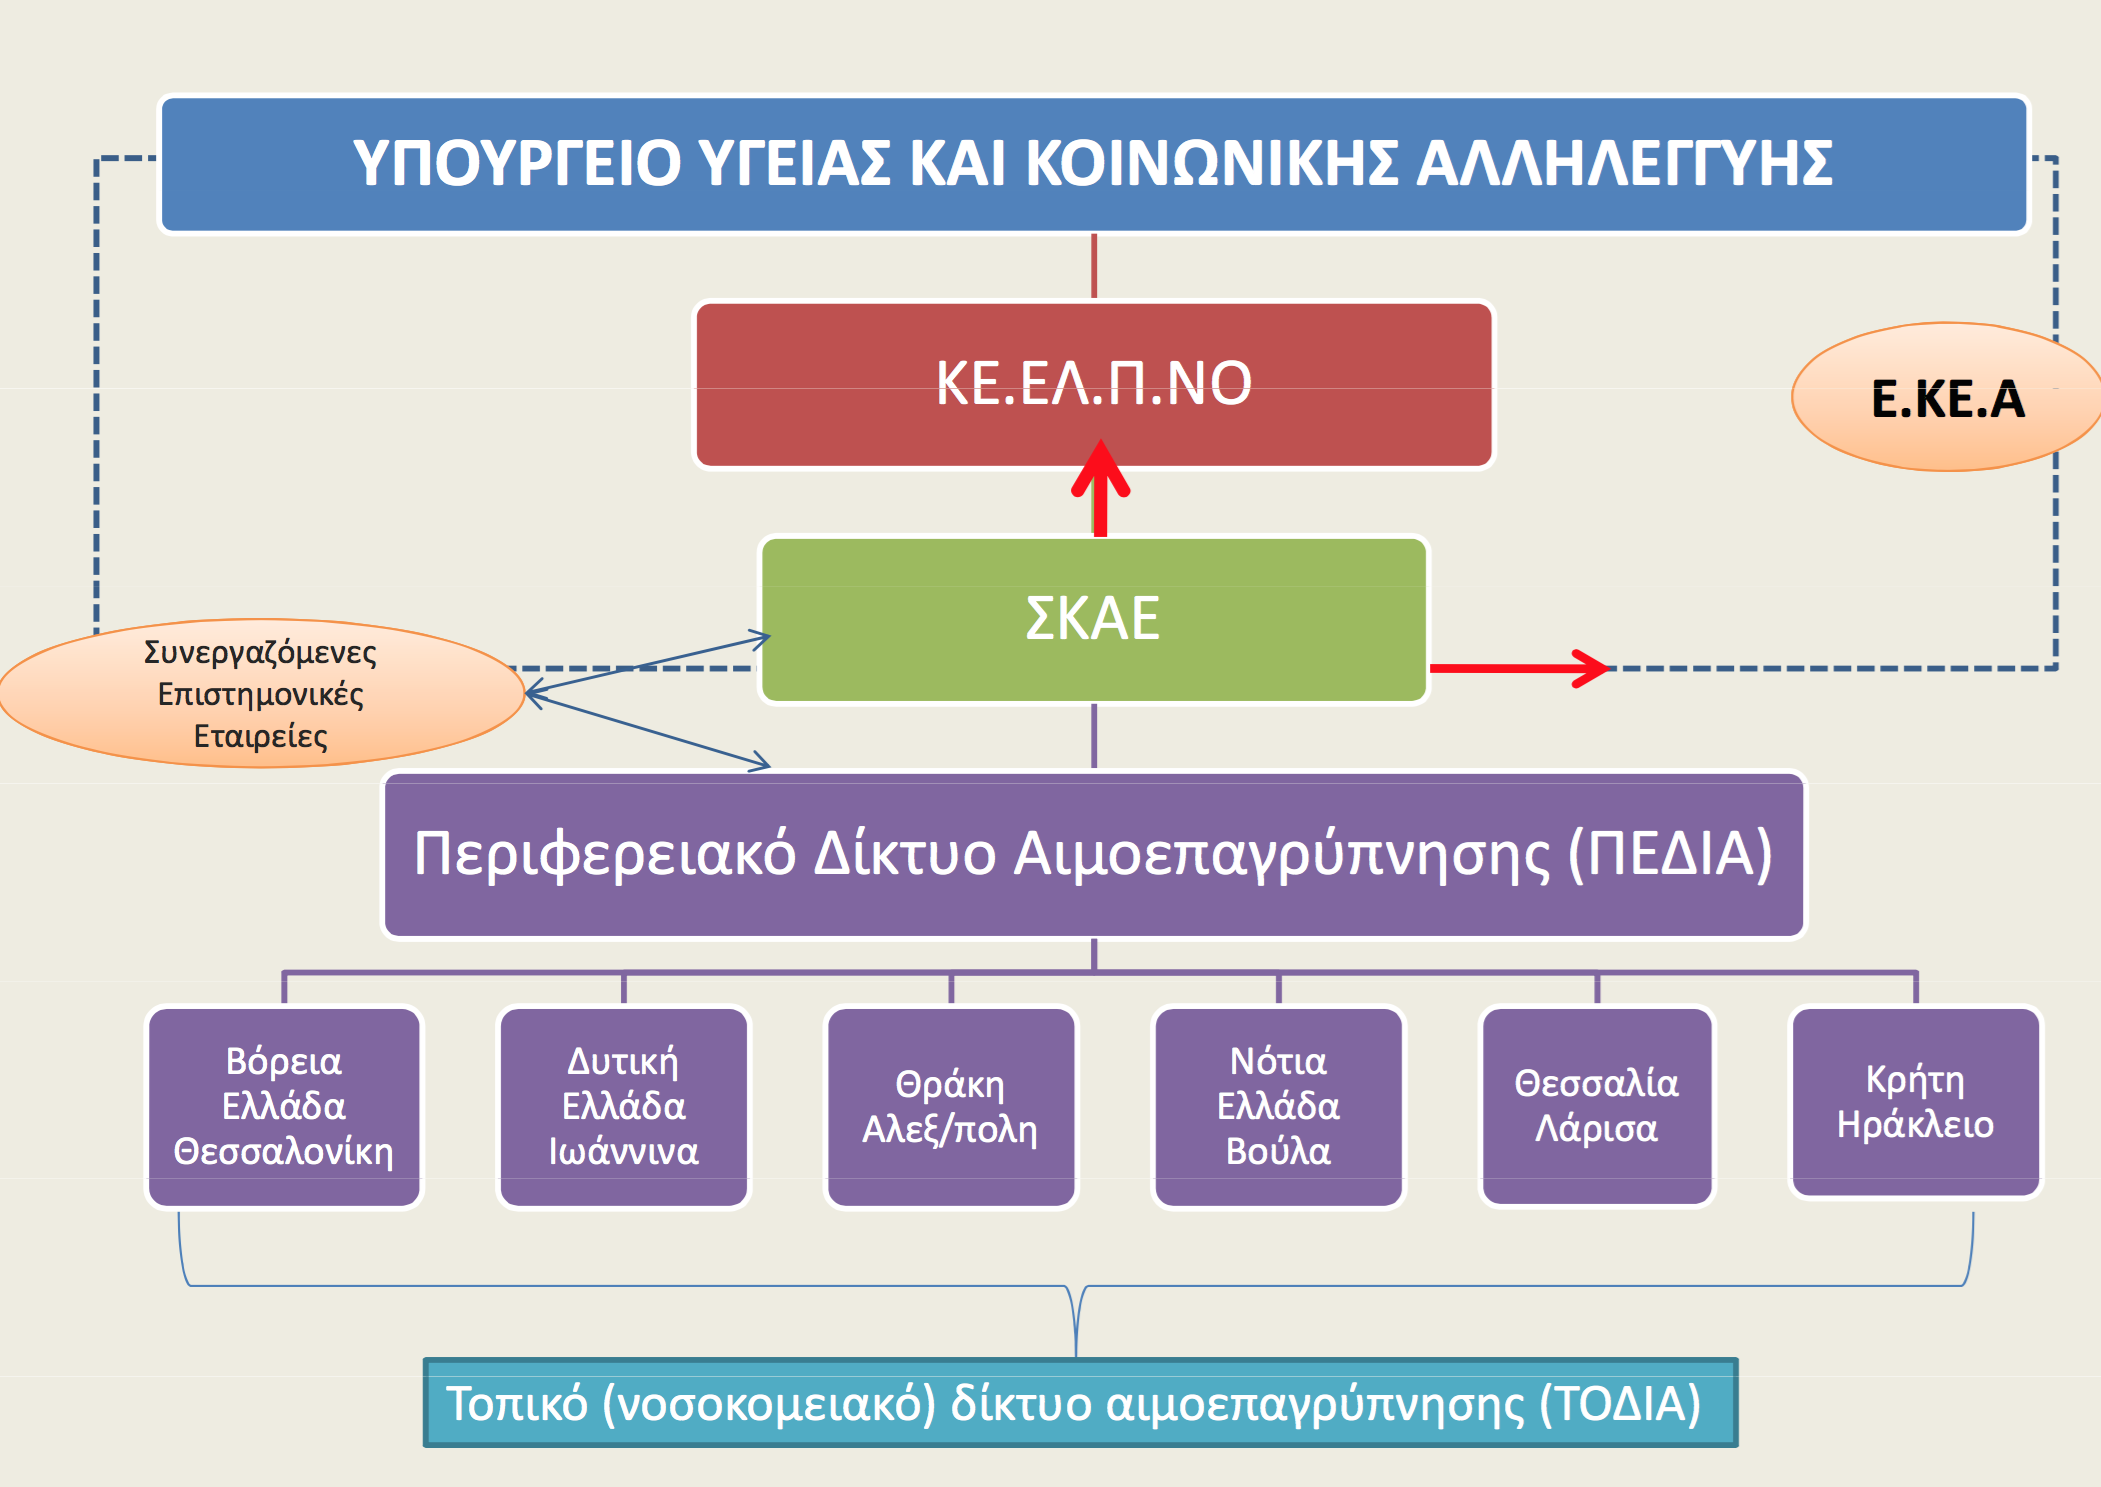
\includegraphics[width=0.7\textwidth]{SKAE_diagram.jpg}
	    \caption{Διάγραμμα λειτουργίας}
	    \label{fig:SKAE_diagram}
\end{figure}	

Οι βασικές λειτουργίες του ΣΚΑΕ είναι οι εξής:
\begin{itemize}
		\item Η συνεχής επιδημιολογική επιτήρηση των λοιμώξεων που μεταδίδονται με το αίμα. Αυτό επιτυγχάνεται με χρήση συστημάτων ανιχνευσιμότητας σε όλα τα στάδια της αιματικής αλυσίδας. Σε περίπτωση εντοπισμού πιθανών μολυσματικών μονάδων, ακολουθεί η άμεση απόσυρση τους. Πραγματοποιούνται διαρκώς αναδρομικοί έλεγχοι, με σκοπό να μειωθούν στο ελάχιστο τα πιθανά λάθη. 
		\item	Η επιδημιολογική επιτήρηση ανεπιθύμητων αντιδράσεων και συμβάντων σχετικών με την μετάγγιση αίματος. Οι παρατηρήσεις αυτές ακολουθούνται από αναφορές στις αρμόδιες αρχές και διαμόρφωση προτάσεων με αποτελεσματικά διορθωτικά μέτρα, τις οποίες ακολουθούν τα νοσοκομεία και τα κέντρα αιμοδοσίας.  
		\item Η επαγρύπνηση για ανεπιθύμητες αντιδράσεις, ατυχήματα, βλάβες και επιπλοκές στην διάρκεια και μετά από την αιμοδοσία. Άμεση προϋπόθεση του συστήματος επαγρύπνησης είναι η ύπαρξη συστημάτων άμεσης ετοιμότητας εγέρσεων συναγερμών και η αποτελεσματική και αξιόπιστη δυνατότητα διαχείρισης κρίσεων.  Το ΣΚΑΕ ενημερώνει τακτικά την ιατρική κοινότητα για τις εξελίξεις με δημοσιεύσεις και εκδόσεις. 
		\end{itemize}
Το ΣΚΑΕ έχει αναπτύξει πλήρεις και αποτελεσματικές μεθόδους εργασίας, με βάση τις κατευθυντήριες οδηγίες της Ευρωπαϊκής Ένωσης και του Διεθνούς Οργανισμού υγείας(WHO). 

	Όσον αφορά στις λοιμώξεις που μεταδίδονται με το αίμα εφαρμόζεται αναλυτική καταγραφή των οροθετικών αιμοδοτών για HIV, HBV, HCV, σύφιλη, HTLV καθώς και ανάλυση 
των επιδημιολογικών δεδομένων σε σχέση με τις μονάδες αίματος, την Υπηρεσία Αιμοδοσίας, τα δημογραφικά χαρακτηριστικά των αιμοδοτών (φύλο, ηλικία, τόπος διαμονής, οικονομικό και μορφωτικό επίπεδο), την κατηγορία αιμοδοτών (εθελοντές, συγγενείς, στρατιώτες) και την αιμοδοτική συχνότητα (αιμοδότες πρώτης φοράς, σποραδικοί και τακτικοί). Επιπλέον καταγράφονται αναλυτικά τα δεδομένα για ποιοτικούς ελέγχους, πιστοποιήσεις ποιότητας, δείκτες συλλογής και ελέγχου του αίματος ανά Υπηρεσία Αιμοδοσίας και διαχείρισης ανθρώπινου δυναμικού. Με βάση τους εγγεγραμμένους αιμοδότες πραγματοποιείται συνεχής παρακολούθηση και χαρτογράφηση των ρετροϊκών λοιμώξεων και των ηπατιτίδων στον αιμοδοτικό πληθυσμό. Οι μεθόδοι ορολογικού και μοριακού ελέγχου του αίματος για λοιμώξεις διευρύνονται διαρκώς. Πραγματοποιείται πλήρης  καταγραφή δεδομένων για ποιοτικό έλεγχο, πιστοποίηση ποιότητας, δείκτες συλλογής και ελέγχου του αίματος ανά Υπηρεσία Αιμοδοσίας και διαχείρισης ανθρώπινου δυναμικού. Το ΣΚΑΕ έχει καθιερώσει πρωτόκολλα ανιχνευσιμότητας για λοιμώξεις που αναφέρονται ύστερα από μετάγγιση αίματος καθώς και πρωτόκολλα αναδρομικού ελέγχου ληπτών δυνητικά μολυσμένου αίματος τα οποία είναι καθολικά και χρησιμοποιούνται σε όλες τις υπηρεσίες υγείας. Τέλος διεξάγονται διαρκώς μελέτες κόστους – ωφέλειας για τα μέτρα πρόληψης της διασποράς λοιμωδών νόσων με το αίμα και τα προϊόντα του αίματος καθώς και έρευνα πάνω στις νέες λοιμώξεις (Ηπατίτιδα Ε κλπ). 

	Στον τομέα των ανεπιθύμητων αντιδράσεων και τα ανεπιθύμητων συμβάντων κατά και μετά την αιμοδοσία καταγράφονται αναλυτικά όλες οι ανεπιθύμητες αντιδράσεις και τα συμβάντα που προκύπτουν κατά την αιμοδοσία εθελοντών και με βάση τα καταγεγραμμένα γεγονότα αναλύονται οι πληροφορίες που προκύπτουν πάνω στον τύπο και στην σοβαρότητα των αντίδρασεων/ συμβάντων. Με βάση τις αναλύσεις αυτές προκύπτουν κάποια συμπεράσματα και προτάσεις για βελτίωση της ποιότητας των αιμοδοσιών και δίνονται κατευθυντήριες αρχές στα νοσοκομεία και στα αιμοδοτικά κέντρα.
	
	Οι μέθοδοι εργασίας αναφορικά με τις ανεπιθύμητες αντιδράσεις και τα ανεπιθύμητα συμβάντα σχετικά με τη μετάγγιση αίματος και προϊόντων αίματος περιλαμβάνουν σε πρώτο στάδιο την καταγραφή ανεπιθυμήτων αντιδράσεων, που σχετίζονται με λοιμογόνους παράγοντες (ιογενείς, βακτηριακοί, παρασιτικοί παράγοντες) καθώς και αυτών που σχετίζονται με μη λοιμογόνουες παράγοντες, ανεξάρτητα από την σοβαρότητα των αντιδράσεων. Επιπλέον καταγράφονται τα ανεπιθύμητα σοβαρά και «παρ’ ολίγον» συμβάματα και τα σφάλματα των μεταγγίσεων χωρίς σύμβαμα», που μπορεί να επηρεάσουν την ασφάλεια και την ποιότητα του μεταγγιζόμενου προϊόντος αίματος, σε όλες τις διαδικασίες της συλλογής, του ελέγχου, της επεξεργασίας, της αποθήκευσης και της διανομής προϊόντων αίματος. Το ΣΚΑΕ διαμορφώνει τα δελτία αναφοράς των ανεπιθύμητων αντιδράσεων και ανεπιθύμητων συμβάντων και τις οδηγίες διερεύνησης και αντιμετώπισης τους , σύμφωνα με τις Ευρωπαϊκές Οδηγίες και τις συστάσεις του Διεθνούς Δικτύου Αιμοεπαγρύπνησης. Οι πληροφορίες σχετικά με τις ανεπιθύμητες αντιδράσεις και τα ανεπιθύμητα συμβάντα αναλύονται διεξοδικά ανάλογα με τον τύπο της αντίδρασης, τη συσχέτισης με τη μετάγγιση, τη σοβαρότητα και την έκβαση της αντίδρασης και το προϊόν αίματος (ερυθρά, πλάσμα, αιμοπετάλια). Τέλος το ΣΚΑΕ συλλέγει, αναλύει και καταγράφει την ποιότητας των ελληνικών αναφορών για τις μεταδιδόμενες με τη μετάγγιση λοιμώξεις συγκριτικά με τις απαιτήσεις αιμοεπαγρύπνησης και τις συστάσεις των διεθνών οργανισμών.
	
	Στην συνέχεια παρουσιάζονται στοιχεία τα οποία έχουν προκύψει από μακροχρόνιες μελέτες του ΣΚΑΕ και αφορούν τις ελληνικές αιμοδοσίες. \cite{ΚΕΕΛΠΝΟ2015}
	Έπειτα από εκτεταμένες μελέτες και επιτηρήσεις έχουν προκύψει τα εξής στοιχεία τα οποία αφορούν στην χώρα μας με βάση τις βασικές επιτηρήσεις του ΣΚΑΕ. Στο σχήμα \ref{fig:statistics1}  παρουσιάζονται τα αποτελέσματα της οροεπικράτησης των λοιμώξεων που αφορούν ελεγχθείσες μονάδες ολικού αίματος και αιμοπεταλιαφαίρεσης το διάστημα των ετών 1996-2013. Στο σχήμα 2 \ref{fig:statistics2} παρουσιάζεται η μέση ετήσια μεταβολή ορολογικών δεικτών κατά στο διάστημα των ετών 2003-2013.
	\begin{figure}[h!]
	    \centering
	    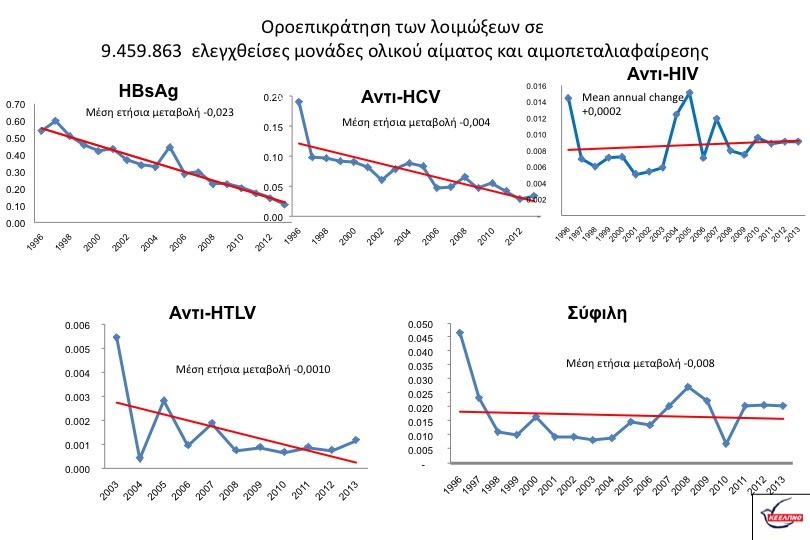
\includegraphics[width=0.7\textwidth]{statistics1.jpg}
	    \caption{Οροεπικράτηση λοιμώξεων σε 9.459.863 ελεγχθείσες μονάδες αίματος και αιμοπεταλιαφαίρεσης.}
	    \label{fig:statistics1}
\end{figure}	
\begin{figure}[h!]
	    \centering
	    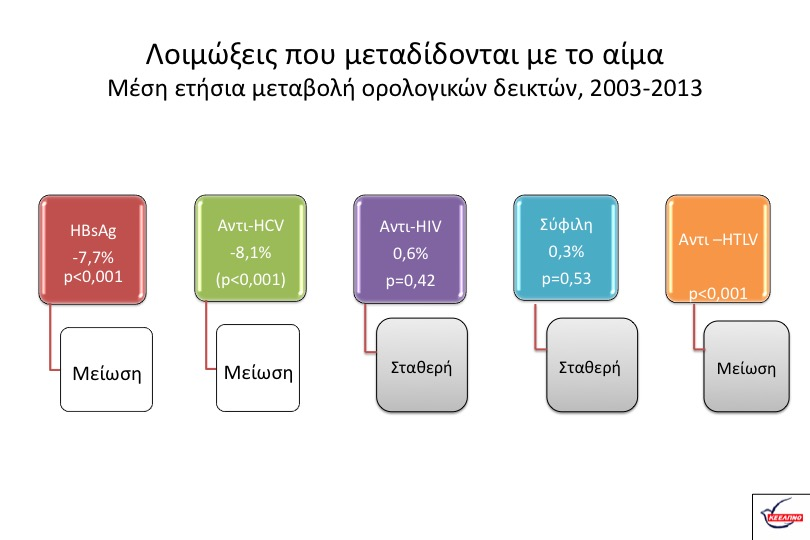
\includegraphics[width=0.7\textwidth]{statistics2.jpg}
	    \caption{Μέση μεταβολή των ορολογικών δεικτών των λοιμώξεων που μεταδίδονται με το αίμα}
	    \label{fig:statistics2}
\end{figure}	
	Η κατανομή και η ανάλυση των ανεπιθύμητων αντιδράσεων σχετικά με τη μετάγγιση ασθενών το έτος 2013 φαίνονται στο \ref{fig:statistics3}. Το έτος 2013 δηλώθηκαν, μελετήθηκαν και παρουσιάσθηκαν 1092 ανεπιθύμητες αντιδράσεις κατά τη μετάγγιση 729456 προϊόντων αίματος. Η συχνότητα των σοβαρών αντιδράσεων κατά τη μετάγγιση είναι 1/9994 προϊόντα. Κατά τα έτη 1997-2013, δηλώθηκαν επτά θάνατοι σχετικά με τη μετάγγιση 8972722 προϊόντων αίματος, συχνότητα 1/281817 προϊόντα με κύρια αίτια: ΑΒΟ ασυμβατότητα, TRALI, βακτηριακή επιμόλυνση.
\begin{figure}[h!]
	    \centering
	    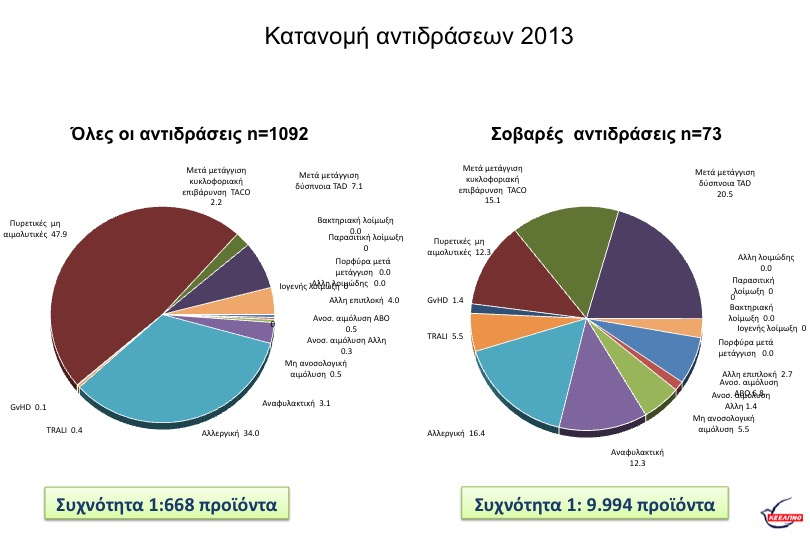
\includegraphics[width=0.7\textwidth]{statistics3.jpg}
	    \caption{Κατανομή αντιδράσεων}
	    \label{fig:statistics3}
\end{figure}
Στο σχήμα \ref{fig:statistics4} παρουσιάζονται διαγραμματικά οι ανεπιθύμητες αντιδράσεις σχετικές  με την αιμοδοσίας. Πιο συγκεκριμένα δηλώθηκαν 148 ανεπιθύμητες αντιδράσεις που αφορούσαν σε σύνολο μεταγγίσεων 44611 μονάδων ερυθρών αιμοσφαιρίων. Καταγράφηκαν (σε ποσοστά επί τοις εκατό) 0.22 πυρετικές, 0.13 αλλεργικές, 0.13 αλλοανοσοποίηση και 0.6 άλλης αιτιολογίας αντίδρασης. Τέλος, στο σχήμα \ref{fig:statistics5} παρουσιάζεται ποσοστιαία ο αριθμός των συμβάντων που  έλαβαν χώρα πριν και κατά την διάρκεια της αιμοδοσίας.
\begin{figure}[h!]
	    \centering
	    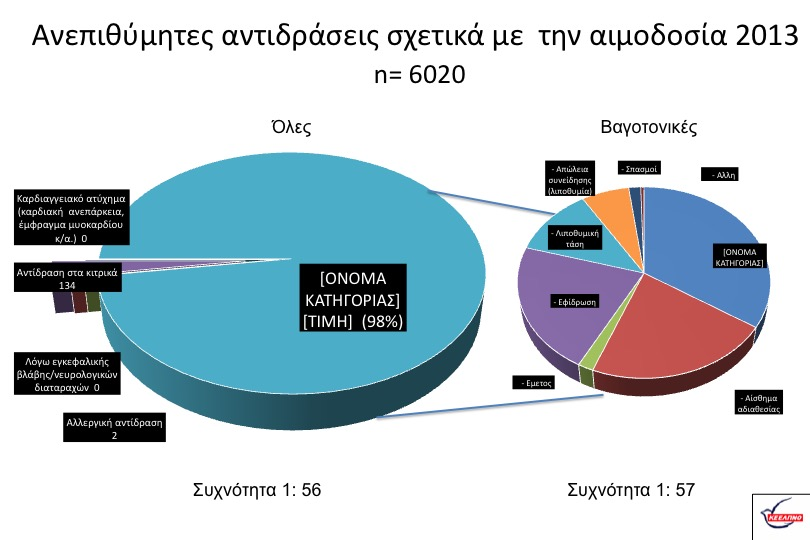
\includegraphics[width=0.7\textwidth]{statistics4.jpg}
	    \caption{Ανεπιθύμητες αντιδράσεις σχετικά με την αιμοδοσία 2013}
	    \label{fig:statistics4}
\end{figure}
\begin{figure}[h!]
	    \centering
	    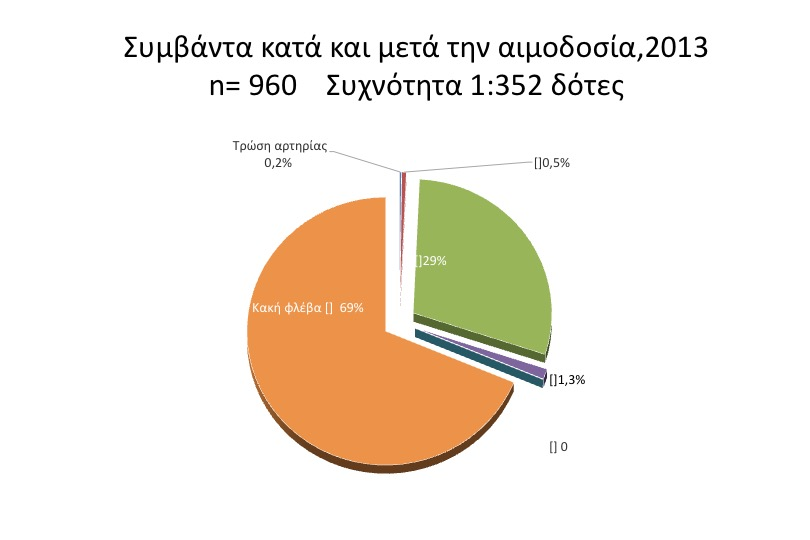
\includegraphics[width=0.7\textwidth]{statistics5.jpg}
	    \caption{ Συμβάντα κατά και μετά την αιμοδοσία, 2013}
	    \label{fig:statistics5}
\end{figure}

\graphicspath{ {Figures/system_analysis/} }

\chapter{Ανάλυση και σχεδιασμός του συστήματος LifeDonor}\label{ch:Analysis of LifeDonor}
\section{Λειτουργικές απαιτήσεις}

	Οι απαιτήσεις ενός συστήματος αποτελούν τη βάση των συστημάτων λογισμικού. Ουσιαστικά, είναι η περιγραφή των υπηρεσιών που πρέπει να παρέχει ένα σύστημα λογισμικού και οι περιορισμοί υπό τους οποίους πρέπει αυτές να λειτουργούν. Διακρίνονται σε δύο βασικές κατηγορίες τις λειτουργικές απαιτήσεις (functional requirements) και τις μη λειτουργικές απαιτήσεις(non functional requirements). 
	
	Οι λειτουργικές απαιτήσεις προσδιορίζουν τα βασικά χαρακτηριστικά του συστήματος και την λειτουργία του από την άποψη του ίδιου του προϊόντος και των χρηστών του. Στον όρο λειτουργία του συστήματος συμπεριλαμβάνεται οι συνολικές είσοδοι, η συμπεριφορά και οι έξοδοι του συστήματος. Στο σύστημα που υλοποιούμε, οι λειτουργικές απαιτήσεις χρησιμοποιούνται για να περιγράψουν ειδικές λειτουργίες που καθορίζουν αυτά τα οποία αναμένουμε να πετύχει το σύστημα. Αν και αναφέρονται ως "απαιτήσεις", στην πραγματικότητα αποτελούν μια μορφή σχεδιασμού, υψηλού επιπέδου. Οι λειτουργικές απαιτήσεις συχνά προσδιορίζονται ως λειτουργικές προδιαγραφές,» και ο όρος περιγραφή αποτελεί συνώνυμο του σχεδιασμού. Οι λειτουργικές απαιτήσεις είναι ουσιαστικά το "τι" λειτουργία θέλουμε να επιτελεί το σύστημα, χωρίς να παρέχουμε καμία πληροφορία για το "πως".
	
	Οι μη λειτουργικές απαιτήσεις είναι οι απαιτήσεις που καθορίζουν τα κριτήρια που χρησιμοποιούνται για να κρίνουν την λειτουργία του συστήματος και κατά επέκταση  αν είναι επιτυχημένο ή όχι, για αυτό και συχνά αποκαλούνται και ιδιότητες του. Επεξεργάζονται τα χαρακτηριστικά απόδοσης του, και μπορούν επίσης να περιγράψουν τις πτυχές του συστήματος που δεν σχετίζονται με την εκτέλεση του, αλλά με την εξέλιξη του στο πέρασμα του χρόνου. Οι βασικές συνήθεις κατηγορίες των μη λειτουργικών απαιτήσεων σχετίζονται με την ασφάλεια( ασφαλή πρόσβαση σε δεδομένα αλλά και σε hardware), την απόδοση ( ορίζουν χαρακτηριστικά που έχουν να κάνουν με την ταχύτητα και την ανταπόκριση του συστήματος) και την επεκτασιμότητα (σχετίζονται με το μέγεθος του συστήματος). Γενικότερα, οι μη λειτουργικές απαιτήσεις καθορίζουν το πώς πρέπει να είναι ένα σύστημα, σε αντίθεση με τις λειτουργικές απαιτήσεις που καθορίζουν τι πρέπει να κάνει ένα σύστημα. Οι λειτουργικές απαιτήσεις ανήκουν στο κομμάτι σχεδιασμού και ανάλυσης του συστήματος ενώ οι μη λειτουργικές απαιτήσεις ανήκουν στο κομμάτι της αρχιτεκτονικής του συστήματος.
	
	\subsection{Λειτουργίες εφαρμογής (web, mobile)}
Οι χρήστες του συστήματος χωρίζονται σε τρεις μεγάλες ομάδες χρηστών.

		\begin{enumerate}

			\item Εθελοντές αιμοδότες
			\item Εγκεκριμένοι χρήστες/διαχειριστές των συστημάτων αιμοδοσίας
			\item Υπέρ-Διαχειριστές του συστήματος

		\end{enumerate}
		
		Οι εθελοντές αιμοδότες αποτελούν την βασική κατηγορία χρηστών καθώς πραγματοποιούν συνεχή και εκτεταμένη χρήση των υπηρεσιών του συστήματος, τόσο στο επίπεδο της εφαρμογής έξυπνου κινητού όσο και μέσω του web portal. Οι εγκεκριμένοι χρήστες/διαχειριστές των συστημάτων αιμοδοσίας χρησιμοποιούν αποκλειστικά το web portal το οποίο βρίσκεται στο υπολογιστικό νέφος για ολοκληρωμένη διαχείριση ενός πλήρους κύκλου αιμοδοσίας. Οι λειτουργίες που μπορεί να επιτελέσει κάθε ομάδα χρηστών καθώς και οι λειτουργικές απαιτήσεις του συστήματος αναλύονται με λεπτομέρειες στην συνέχεια.
		
		\subsubsection{Mobile} \label{sssec:functional_requirements_mobile}
			Επιγραμματικά, οι λειτουργικές απαιτήσεις της εφαρμογής έξυπνου κινητού είναι οι εξής:
			
			\begin{itemize}
				\item Δυνατότητα εγγραφής στο σύστημα ως εθελοντής αιμοδότης με χρήση του αριθμού μητρώου κοινωνικής ασφάλισης (Α.Μ.Κ.Α.).
				\item Δυνατότητα σύνδεσης στο σύστημα αν έχει πραγματοποιήσει ήδη έγγραφή στο παρελθόν.
				\item Δυνατότητα προβολής γεγονότων αιμοδοσίας.
				\item Δυνατότητα λήψης ειδοποιήσεων (push notifications) όταν δημιουργείται κάποιο νέο γεγονός αιμοδοσίας για το οποίο ο εθελοντής αιμοδότης πληρεί τα απαραίτητα κριτήρια.
				\item Δυνατότητα αποδοχής, απόρριψης ή αναβολής της ειδοποίησης για το γεγονός αιμοδοσίας.
				\item Δυνατότητα διαχείρισης ραντεβού για αιμοδοσία (δημιουργία νέου ραντεβού, μετάθεση , προβολή, ακύρωση).
				\item Δυνατότητα προσθήκης και συγχρονισμού των ραντεβού αιμοδοσίας στο ημερολογίου του χρήστη.
				\item Δυνατότητα ενημέρωσης σχετικά με το υπολειπόμενο διάστημα που πρέπει να παρέλθει ώστε ο εθελοντής να είναι σε θέση να συμμετέχει σε μία νέα αιμοδοσία.
				\item Δυνατότητα να κερδίσει πόντους και εμβλήματα βάση των αιμοδοσιών του (gamification system) και να τα μοιραστεί στα μέσα κοινωνικής δικτύωσης.
				\item Δυνατότητα να μοιραστεί και να δημοσιεύσει στοιχεία στα μέσα κοινωνικής δικτύωσης σε κάθε στάδιο της αιμοδοσίας.
				\item Δυνατότητα δημιουργίας έκκλησης για αίμα σε περίπτωση ανάγκης ατόμων του στενού κύκλου χρήστη και δημοσίευσης του στα μέσα κοινωνικής δικτύωσης.
				\item Δυνατότητα διαχείρισης προφίλ χρήστη.

			\end{itemize}

			\subsubsection{Web Portal} \label{sssec:functional_requirements_web}
			
				Το web portal που βρίσκεται στο υπολογιστικό νέφος χρησιμοποιείται από όλες τις ομάδες χρηστών. Όσον αφορά στους εθελοντές αιμοδότες ισχύουν οι ίδιες λειτουργικές απαιτήσεις όπως στην εφαρμογή του έξυπνου κινητού οι οποίες και αναλύθηκαν παραπάνω στο \ref{sssec:functional_requirements_mobile}. Όσον αφορά στους χρήστες/διαχειριστές των κέντρων αιμοδοσίας έχουμε τις παρακάτω λειτουργικές απαιτήσεις:
				
				\begin{itemize}
					\item Δημιουργία νέων γεγονότων αιμοδοσίας.
				%	\item Αποστολή ειδοποιήσεων στους εθελοντές αιμοδότες βάση των γεγονότων αιμοδοσίας, των αναγκών και των κριτηρίων αποδοχής.
					\item Προβολή στατιστικών ανά έτος σχετικά με τις ειδοποιήσεις που στάλθηκαν από το συγκεκριμένο κέντρο αιμοδοσίας και την ανταπόκριση των χρηστών (αποδοχή, απόρριψη, άνοιγμα ειδοποίησης, ολοκλήρωση αιμοδοσίας).
					\item Διαχείριση των ραντεβού για αιμοληψία.
					\item Διαχείριση του προφίλ του κέντρου αιμοδοσίας.
				%	\item Εισαγωγή δεδομένων από το τοπικό τους σύστημα στο κεντρικό σύστημα μας που βρίσκεται στο υπολογιστικό νέφος
					\item Δυνατότητα εγγραφής στο σύστημα νέου εθελοντή αιμοδότη.
					\item Δυνατότητα καταχώρησης της ολοκλήρωσης της αιμοδοσίας.
					\item Δυνατότητα ελέγχου τήρησης προϋποθέσεων καταλληλότητας εθελοντή αιμοδότη.
				\end{itemize}
				Όσον αφορά στους υπέρ-διαχειριστές του συστήματος έχουμε τις παρακάτω λειτουργικές απαιτήσεις:
				\begin{itemize}
					\item Δυνατότητα διαχείρισης λογαριασμών χρηστών.
					\item Προβολή στατιστικών για τους χρήστες του συστήματος.
				\end{itemize}

	
\section{Σενάρια χρήσης}

	Η διαδικασία της μοντελοποίησης, δηλαδή ο αναλυτικός σχεδιασμός ενός συστήματος, πριν από την υλοποίηση του είναι ένα πολύ βασικό στάδιο κατά την ανάπτυξη εφαρμογών. Ένα σύστημα μοντελοποιείται επιτυχώς όταν οι λειτουργικότητες του συστήματος έχουν περιγραφεί πλήρως και ορθώς, έχουν καλυφθεί οι ανάγκες των τελικών χρηστών και υποστηρίζεται η επεκτασιμότητα του συστήματος. 
	Η ενοποιημένη Γλώσσα Μοντελοποίησης (UML) είναι μια τυπική γλώσσα για τη σύνταξη λεπτομερών σχεδίων λογισμικού. Η UML μπορεί να χρησιμοποιηθεί για να απεικονίσει, να προσδιορίζει,να κατασκευάσει και να τεκμηριώσει τα προϊόντα του συστήματος εντάσεως λογισμικού.\cite{Booch2005}. Δεν αποτελεί απλώς έναν κατάλογο από διαγράμματα, αλλά είναι μια γλώσσα αναπαράστασης γνώσης. Αυτό συνεπάγεται ότι κάθε στοιχείο διαγράμματος, π.χ. κουτί, βέλος, κύκλος, ορθογώνιο κ.λ.π., υποστηρίζεται από συγκεκριμένους κανόνες σύνταξης και σημασιολογία.
	 Επιλέξαμε να μοντελοποιήσουμε το σύστημα μας με χρήση της γλώσσας UML για τους εξής λόγους:
	 
	 \begin{itemize}
	 \item Είναι ένα βιομηχανικό πρότυπο από τον διεθνή, ανοιχτό και μη κερδοσκοπικό οργανισμό εταιριών Object Management Group (OMG).
	 \item Η UML είναι χτισμένη πάνω σε θεμελιώσεις αντικειμενοστραφείς έννοιες, όπως η κλάση, με αποτέλεσμα να υποστηρίζει καλύτερα την ανάπτυξη και τον σχεδιασμό του αντικειμενοστραφούς λογισμικού.
	 \item Δίνει έμφαση στην ανάλυση των σεναρίων χρήσης, το οποίο είναι ένα πολύτιμο εργαλείο για την παρακολούθηση των σταδίων μιας διαδικασίας από την οπτική γωνία του χρήστη.
	 \item Δίνει στον σχεδιαστή την δυνατότητα να παρουσιάσει όσο λεπτομερώς επιθυμεί αυτός τις περιγραφές του συστήματος.
	 \item Τμηματοποιεί τον σχεδιασμό του συστήματος με αποτέλεσμα να αυξάνεται η επεκτασιμότητα του.
\end{itemize}	 

	Η UML 2.0 ορίζει δεκατρείς τύπους διαγραμμάτων, τα οποία μπορούν να χωριστούν σε δύο βασικές κατηγορίες:
	
	\begin{itemize}
		\item Τα διαγράμματα στατικής δομής, τα οποία δείχνουν τα πράγματα τα οποία απαρτίζουν το σύστημα που μοντελοποιείται και δεν αλλάζουν στο πέρασμα του χρόνου, για παράδειγμα τις κλάσεις, τα αντικείμενα κλπ. Στα διαγράμματα δομής ανήκουν: τα διαγράμματα κλάσεων, τα διαγράμματα αντικειμένων, τα ψηφιδικά διαγράμματα, τα διαγράμματα σύνθετης δομής, τα διαγράμματα πακέτου και τα διαγράμματα διάταξης.
		
		\item Τα διαγράμματα συμπεριφοράς, τα οποία δίνουν έμφαση στο τι πρέπει να γίνει στο σύστημα που μοντελοποιούμε, όπως τις αλληλεπιδράσεις με τους χρήστες, τις διάφορες καταστάσεις του συστήματος κλπ. Διαγράμματα συμπεριφοράς αποτελούν τα ακόλουθα: τα διαγράμματα χρήσης, τα διαγράμματα δραστηριότης, τα διαγράμματα καταστάσεων μηχανής, τα ακολουθιακά διαγράμματα, τα συνεργατικά διαγράμματα και τα διαγράμματα χρονισμού.
	\end{itemize}
	
Κάθε ένα από τα παραπάνω διαγράμματα βλέπει το σύστημα από μια διαφορετική οπτική γωνία, π.χ. τα διαγράμματα χρήσης δείχνουν πώς οι χρήστες αλληλεπιδρούν με το σύστημα, τα διαγράμματα κλάσης δείχνουν τις κλάσεις του συστήματος και τις σχέσεις μεταξύ τους κλπ.
	
		Η πρακτική της ανάλυσης με σενάρια χρήσης τυποποιήθηκε για πρώτη φορά από τον Jacobson το 1994, ο οποίος περιέγραψε το σενάριο χρήσης σαν "μία σειρά από συναλλαγές που σχετίζονται ως προς την συμπεριφορά και εκτελούνται από έναν δράστη που βρίσκεται σε επικοινωνία με το σύστημα με σκοπό την παροχή κάποιας μετρήσιμης αξίας στον δράστη" \cite{Jacobson} . Ένα σενάριο χρήσης είναι μία συλλογή από πιθανά σενάρια μεταξύ του συστήματος και των εξωτερικών του δραστών. Κάθε σενάριο χρήσης χαρακτηρίζεται από τον στόχο που έχει ο κύριος δράστης του. Ο στόχος αυτός μπορεί να επιτευχθεί ή όχι. Τα σενάρια χρήσης αποτελούν ένα πολύ διαδεδομένο και πολύτιμο εργαλείο για την πλήρη αποτύπωση των λειτουργικών απαιτήσεων του συστήματος. Οι λειτουργικές απαιτήσεις μπορούν να εκφραστούν είτε με μορφή κειμένου, είτε με μορφή πίνακα. Επιλέξαμε να χρησιμοποιήσουμε την μορφή πίνακα, καθώς έχει πιο αυστηρή δομή με αποτέλεσμα να μειώνονται οι ασυνέπειες και οι περιττές πληροφορίες. \cite{Cockburn2000} και πιο συγκεκριμένα την μονή στήλη πρότυπο \cite{Cockburn2000} :
 
 
\begin{table}[H]
	\begin{center}
	    \begin{tabular}{|p{\dimexpr \linewidth-2\tabcolsep}|}
	    \hline
	    \rowcolor{grayy}
	    \textbf{Όνομα σεναρίου χρήσης}
	    \\ \hline    
	    Ο τίτλος του σεναρίου χρήσης, που συνήθως είναι ένα μία πρόταση που περιγράφει τον στόχο του κύριου δράστη.
	    \\ \hline
	    \rowcolor{grayy}
	    \textbf{Στόχος}
	    \\ \hline
 Μία μεγαλύτερη δήλωση η οποία περιγράφει τον στόχο του σεναρίου χρήσης με περισσότερες λεπτομέρειες.
	    \\ \hline
	    \rowcolor{grayy}
	    \textbf{Λεπτομέρειες}
	    \\ \hline
		\textbf{Δράστης:} Είναι οι δράστες που έχουν ως στόχο αυτόν που περιγράφεται από το σενάριο χρήσης.
		\\ \hline
		\textbf{Προϋποθέσεις:} Αυτά που ισχύουν πριν ξεκινήσει να εκτελείται το σενάριο χρήσης. Εφόσον είναι γνωστό ότι μια συνθήκη είναι αληθής, δεν θα ελεγχθεί ξανά κατά την διάρκεια εκτέλεσης του σεναρίου χρήσης. 
		\\ \hline
		\textbf{Ενέργεια ενεργοποίησης:} Καθορίζει ποιο γεγονός εκκινεί το σενάριο χρήσης. Η ενέργεια εκκίνησης αποτελεί το πρώτο βήμα του σεναρίου χρήσης. 
		\\ \hline
		\rowcolor{grayy}    
	    \textbf{Ροή γεγονότων}
	    \\ \hline
		\textbf{Κύρια ροή γεγονότων:}
		Η κύρια ροή γεγονότων περιγράφει την περίπτωση που όλα βαίνουν αισίως. Είναι μια σειρά από αριθμημένα βήματα, όπου το κάθε βήμα είναι μία ρητή εντολή- μετάβαση.
		\\ \hline
		\textbf{Επεκτάσεις:} 
Οι επεκτάσεις περιγράφουν τι μπορεί να συμβεί και με διαφορετικό τρόπο κατά την διάρκεια εκτέλεσης του επιτυχημένου σεναρίου. Μπορούν να οδηγήσουν σε επιτυχία ή σε αποτυχίες. Κάθε επέκταση αποτελείται από δύο διαφορετικά μέρη:
 \begin{itemize}
 \item Τις προϋποθέσεις κάτω από τις οποίες το σύστημα υιοθετεί μία διαφορετική συμπεριφορά. Μετά από αυτές τοποθετείται μία άνω και κάτω τελεία (:).
 \item Ο χειρισμός της επέκτασης που είναι μία ακολουθία από βήματα που απαιτούνται λόγω των προϋποθέσεων που υπάρχουν.
 \end{itemize}
		\\ \hline
		\textbf{Παραλλαγές:}
		 Οι παραλλαγές κάποιου βήματος από το επιτυχημένο σενάριο υπάρχουν επειδή ενώ αυτό που συμβαίνει σε κάποιο βήμα είναι πάντα το ίδιο υπάρχουν πολλοί τρόποι να το κάνουμε.
		 \\ \hline

	    \end{tabular}
	    \caption{Σενάριο χρήσης εγγραφής αιμοδότη}
		\label{tab:use_case_sample_table}
	\end{center}
\end{table}
 

 
	\subsubsection{Εφαρμογή}
	
	Θα αναπτύξουμε αρχικά τα σενάρια χρήσης της εφαρμογής.
	
- Σενάριο εγγραφής στο σύστημα ως εθελοντής αιμοδότης με χρήση του αριθμού μητρώου κοινωνικής ασφάλισης (Α.Μ.Κ.Α.).
\\*
\begin{table}[H]
	\begin{center}
	    \begin{tabular}{|p{\dimexpr \linewidth-2\tabcolsep}|}
	    \hline
	    \rowcolor{grayy}
	    \textbf{Όνομα σεναρίου χρήσης}
	    \\ \hline    
	    Εγγραφή στο σύστημα.
	    \\ \hline
	    \rowcolor{grayy}
	    \textbf{Στόχος}
	    \\ \hline
	   Ο χρήστης εισάγει τα προσωπικά του δεδομένα με σκοπό να δημιουργήσει το προσωπικό του μοναδικό αιμοδοτικό προφίλ.
	    \\ \hline
	    \rowcolor{grayy}
	    \textbf{Λεπτομέρειες}
	    \\ \hline
		\textbf{Δράστης:} Εθελοντής αιμοδότης.
		\\*
		\textbf{Προϋποθέσεις:} Να διαθέτει αριθμό ΑΜΚΑ.
		\\*
		\textbf{Ενέργεια ενεργοποίησης:} Μετάβαση στην sign up φόρμα
		\\ \hline
		\rowcolor{grayy}    
	    \textbf{Ροή γεγονότων}
	    \\* 
		\textbf{Κύρια ροή γεγονότων:}
		\begin{enumerate}
			\item	Ο χρήστης πηγαίνει στην επιλογή sign up και εισάγει το ΑΜΚΑ του.
			\item Στην συνέχεια συμπληρώνει την sign up φόρμα και επιλέγει ολοκλήρωση εγγραφής.
			\item Το σύστημα δημιουργεί ένα μοναδικό προφίλ για τον χρήστη, το οποίο εισάγει στην βάση δεδομένων του.
			\item Ο χρήστης ανακατευθύνεται στην αρχική σελίδα 
		\end{enumerate}
		\\ \hline
		\textbf{Επεκτάσεις:} 
		\begin{enumerate}
			\item	Ο χρήστης εισάγει ΑΜΚΑ για το οποίο έχει ήδη δημιουργηθεί κάποιο προφίλ.
			\item Το σύστημα τον ενημερώνει και τον καθοδηγεί ώστε να ανακτήσει τα στοιχεία του.
		\end{enumerate}
		\\*
		\\ \hline
	    \end{tabular}
	    \caption{Σενάριο χρήσης εγγραφής αιμοδότη}
		\label{tab:blood_donor_register}
	\end{center}
\end{table}

- Σύνδεση στο σύστημα αν έχει πραγματοποιήσει ήδη έγγραφή στο παρελθόν.
\\*
\begin{table}[H]	
	\begin{center}
	    \begin{tabular}{|p{\dimexpr \linewidth-2\tabcolsep}|}
	    \hline
	    \rowcolor{grayy}
	    \textbf{Όνομα σεναρίου χρήσης}
	    \\ \hline    
	    Σύνδεση στο σύστημα.
	     \\ \hline
	    \rowcolor{grayy}
	    \textbf{\textbf{Στόχος}}
	    \\ \hline
		Ο χρήστης εισάγει τα στοιχεία του ώστε να μεταφερθεί στον προσωπικό του λογαριασμό.
	    \\ \hline
	    \rowcolor{grayy}
	    \textbf{Λεπτομέρειες}
	    \\ \hline
		\textbf{Δράστης:} Εθελοντής αιμοδότης.
		\\*
		\textbf{Προϋποθέσεις:} Ο χρήστης πρέπει να είναι ήδη εγγεγραμμένος στο σύστημα.
		\\*
		\textbf{Ενέργεια ενεργοποίησης:} Μετάβαση στην sign in φόρμα.
		\\ \hline
		\rowcolor{grayy}    
	    \textbf{Ροή γεγονότων}
	    \\* 
		\textbf{Κύρια ροή γεγονότων:}
		\begin{enumerate}
			\item	Ο χρήστης εισάγει τα στοιχεία του και επιλέγει να συνδεθεί με το σύστημα.
			\item Το σύστημα αποκρίνεται θετικά αν υπάρχει εγγεγραμμένος  χρήστης με αυτά τα στοιχειά στην βάση δεδομένων του συστήματος, αλλιώς απαγορεύει
		την είσοδο στον χρήστη και τυπώνει το αντίστοιχο μήνυμα λάθους.
			\item	Ο χρήστης κατευθύνεται είτε στον προσωπικό του λογαριασμό (σωστή εισαγωγή στοιχειών) είτε του ζητείται να ξαναπροσπαθήσει να εισάγει τα σωστά στοιχεία στην sign in φόρμα.
		\end{enumerate}
		\\ \hline
		\textbf{Επεκτάσεις:}
		\\ \hline
		\begin{itemize}
		\item Ο χρήστης εισάγει μη έγκυρης  μορφής όνομα χρήστη ή κωδικό και επιλέγει να συνδεθεί με το σύστημα.
		\item Το σύστημα εμφανίζει μήνυμα λάθους, χωρίς να επικοινωνήσει με την βάση δεδομένων για ταυτοποίηση.
		\item Το σύστημα αναπροβάλει την φόρμα με μήνυμα οδηγιών στον χρήστη.
		\end{itemize}
	    \end{tabular}
	    \caption{Σενάριο χρήσης σύνδεσης στο σύστημα}
	    \label{tab:user_sign_in} 	
	\end{center}
\end{table}

- Προβολή  γεγονότων αιμοδοσίας.
\\*
\begin{table}[H]	
	\begin{center}
	    \begin{tabular}{|p{\dimexpr \linewidth-2\tabcolsep}|}
	    \hline
	    \rowcolor{grayy}
	    \textbf{Όνομα σεναρίου χρήσης}
	    \\ \hline    
	    Προβολή γεγονότων αιμοδοσίας
	     \\ \hline
	    \rowcolor{grayy}
	    \textbf{\textbf{Στόχος}}
	    \\ \hline
	    	Ο χρήστης θέλει να μπαίνει στην εφαρμογή και να βλέπει όλα τα ενεργά γεγονότα αιμοδοσίας, ταξινομημένα ανά την προτίμηση του(απόσταση, εναπομείνασες ημέρες κλπ) καθώς και τις απαραίτητες πληροφορίες για αυτά (τοποθεσία διεξαγωγής, ημερομηνίες, ομάδα αίματος κλπ)
	    \\ \hline
	    \rowcolor{grayy}
	    \textbf{Λεπτομέρειες}
	    \\ \hline
		\textbf{Δράστης:} Εθελοντής αιμοδότης.
		\\*
		\textbf{Προϋποθέσεις:} Ο χρήστης πρέπει να είναι ήδη εγγεγραμμένος στο σύστημα.
		\\*
		\textbf{Ενέργεια ενεργοποίησης:} Επιλογή της καρτέλας "Γεγονότα αιμοδοσίας".
	    \\ \hline
		\rowcolor{grayy}    
	    \textbf{Ροή γεγονότων}
	    \\ \hline
		\textbf{Κύρια ροή γεγονότων:}
		\begin{enumerate}
			\item	Ο χρήστης επιλέγει την καρτέλα "Γεγονότα αιμοδοσίας".
			\item Το σύστημα φορτώνει από την βάση δεδομένων και την προσωρινή μνήμη τα γεγονότα αιμοδοσίας.
			\item Ο χρήστης επιλέγει και αλλάζει την σειρά ως προς την οποία εμφανίζονται τα γεγονότα ανάλογα με κάποιο κριτήριο.
		\end{enumerate}
				\\ \hline
		\textbf{Επεκτάσεις:}
		   \\ \hline
	    \end{tabular}
	    \caption{Σενάριο χρήσης προβολής γεγονότων αιμοδοσίας}
	    \label{tab:blood_donation_events_show} 
	\end{center}
\end{table}

-Λήψης ειδοποιήσεων (push notifications) όταν δημιουργείται κάποιο νέο γεγονός αιμοδοσίας για το οποίο ο εθελοντής αιμοδότης πληρεί τα απαραίτητα κριτήρια.
\\*
\begin{table}[H]
	\begin{center}
	    \begin{tabular}{|p{\dimexpr \linewidth-2\tabcolsep}|}
	    \hline
	    \rowcolor{grayy}
	    \textbf{Όνομα σεναρίου χρήσης}
	    \\ \hline    
	     Λήψη ειδοποιήσεων (push notifications).
	     \\ \hline
	    \rowcolor{grayy}
	    \textbf{\textbf{Στόχος}}
	    \\ \hline
	 	 Ο εθελοντής αιμοδότης να μπορεί να λαμβάνει ειδοποιήσεις από το σύστημα σχετικά με ενεργές αιμοδοσίες. 
	    \\ \hline
	    \rowcolor{grayy}
	    \textbf{Λεπτομέρειες}
	    \\ \hline
		\textbf{Δράστης:} Εθελοντής αιμοδότης.
		\\*
		\textbf{Προϋποθέσεις:} Ο χρήστης πρέπει να είναι ήδη εγγεγραμμένος στο σύστημα.
		\\*
		\textbf{Ενέργεια ενεργοποίησης:} Δημιουργία νέου γεγονότος αιμοδοσίας.
		\\ \hline
		\rowcolor{grayy}    
	    \textbf{Ροή γεγονότων}
	    \\ \hline
		\textbf{Κύρια ροή γεγονότων:}
		\begin{enumerate}
			\item	Δημιουργείται ένα νέο συμβάν αιμοδοσίας.
			\item Το σύστημα με βάση το business model του αποφαίνεται αν ο χρήστης είναι σε θέση ή όχι να συμμετάσχει στην αιμοδοσία.
			\item Το σύστημα με βάση το αποτέλεσμα του προηγούμενου βήματος στέλνει ή όχι ειδοποίηση στον χρήστη.
			\item Ο χρήστης βλέπει την ειδοποίηση στο κινητό του.
		\end{enumerate}
				\\ \hline
		\textbf{Επεκτάσεις:}
		   \\ \hline
	    \end{tabular}
	    \caption{Σενάριο χρήσης λήψης ειδοποιήσεων}
	    \label{tab:receive_push_notifications} 
	\end{center}
\end{table}

-Αποδοχή, απόρριψη ή αναβολή της ειδοποίησης για το γεγονός αιμοδοσίας.
\\*
\begin{table}[H]
	\begin{center}
	    \begin{tabular}{|p{\dimexpr \linewidth-2\tabcolsep}|}
	    \hline
	    \rowcolor{grayy}
	    \textbf{Όνομα σεναρίου χρήσης}
	    \\ \hline    
	     Διαχείριση ειδοποιήσεων (push notifications).
	     \\ \hline
	    \rowcolor{grayy}
	    \textbf{\textbf{Στόχος}}
	    \\ \hline
	 	 Ο εθελοντής αιμοδότης να μπορεί να διαχειρίζεται αποτελεσματικά τις ειδοποιήσεις από το σύστημα σχετικά με ενεργές αιμοδοσίες, είτε πατώντας αποδοχή,  είτε απορρίπτοντας τες, είτε αναβάλλοντας τες.
	    \\ \hline
	    \rowcolor{grayy}
	    \textbf{Λεπτομέρειες}
	    \\ \hline
		\textbf{Δράστης:} Εθελοντής αιμοδότης.
		\\*
		\textbf{Προϋποθέσεις:} Ο χρήστης πρέπει να είναι ήδη εγγεγραμμένος στο σύστημα.
		\\*
		\textbf{Ενέργεια ενεργοποίησης:} Λήψη νέας ειδοποίησης (push notification).
		\\ \hline
		\rowcolor{grayy}    
	    \textbf{Ροή γεγονότων}
	    \\ \hline
		\textbf{Κύρια ροή γεγονότων:}
		\begin{enumerate}
		
			\item	Λήψη ειδοποίησης από το σύστημα για νέο γεγονός αιμοδοσίας.
			\item  Ο χρήστης επιλέγει μία από τις εξής ενέργειές: αποδοχή, απόρριψη, αναβολή.
			\item Το σύστημα αν ο χρήστης επιλέξει αποδοχή μεταφέρει το γεγονός στην λίστα με τα γεγονότα αιμοδοσίας που έχει αποδεχτεί ο χρήστης, αν επιλέξει απόρριψη μεταφέρει το γεγονός στην λίστα με τα γεγονότα που έχει απορρίψει, αλλιώς προγραμματίζει εκ νέου την αποστολή υπενθύμισης.

		\end{enumerate}
		\\ \hline
		\textbf{Επεκτάσεις:}
		   \\ \hline
	    \end{tabular}
	    \caption{Σενάριο χρήσης διαχείρισης ειδοποιήσεων}
	    \label{tab:manage_notifcations} 
	\end{center}		
\end{table}			
			
			
-Διαχείριση ραντεβού για αιμοδοσία (δημιουργία νέου ραντεβού, μετάθεση , προβολή, ακύρωση).
\\*

\begin{table}[H]
	\begin{center}
	    \begin{tabular}{|p{\dimexpr \linewidth-2\tabcolsep}|}
	    \hline
	    \rowcolor{grayy}
	    \textbf{Όνομα σεναρίου χρήσης}
	    \\ \hline    
	     Διαχείριση ραντεβού για αιμοδοσία.
	     \\ \hline
	    \rowcolor{grayy}
	    \textbf{\textbf{Στόχος}}
	    \\ \hline
	 	 Ο εθελοντής αιμοδότης να αλληλεπιδράσει με το σύστημα των ραντεβού, είτε δημιουργώντας ένα νέο ραντεβού για αιμοδοσία, είτε ακυρώνοντας ένα ήδη υπάρχον, είτε μεταθέτοντας την ημερομηνία ενός ραντεβού.
	    \\ \hline
	    \rowcolor{grayy}
	    \textbf{Λεπτομέρειες}
	    \\ \hline
		\textbf{Δράστης:} Εθελοντής αιμοδότης.
		\\*
		\textbf{Προϋποθέσεις:} Ο χρήστης πρέπει να έχει αποδεχτεί κάποιο γεγονός αιμοδοσίας.
		\\*
		\textbf{Ενέργεια ενεργοποίησης:} Αποδοχή κάποιου γεγονότος αιμοδοσίας ή μετάβαση στο ημερολόγιο.
		\\ \hline

		\rowcolor{grayy}    
	    \textbf{Ροή γεγονότων}
	    \\ \hline
		\textbf{Κύρια ροή γεγονότων:}
		\begin{enumerate}
			\item	 Ο χρήστης μεταφέρεται στο ημερολόγιο των ραντεβού, είτε αποδεχόμενος κάποιο γεγονός αιμοδοσίας, είτε με επιλογή της καρτέλας του ημερολογίου.
			\item  Ο χρήστης βλέπει τις διαθέσιμες ημερομηνίες και ώρες για ραντεβού για πραγματοποίηση αιμοδοσίας, με την επιλογή "Κλείσιμο ραντεβού", καθώς και τα ήδη υπάρχοντα ραντεβού, με τις επιλογές μετάθεση, διαγραφή.
			\item Το σύστημα ανάλογα με τις προηγούμενες ενέργειες του χρήστη κατοχυρώνει τις τελικές αλλαγές.
		\end{enumerate}
		\\ \hline
		\textbf{Επεκτάσεις:}
		   \\ \hline
	    \end{tabular}
	    \caption{Σενάριο χρήσης διαχείρισης ραντεβού αιμοδοσίας}
	    \label{tab:blood_donation_reservation_management} 
	\end{center}
\end{table}	
			
-Προσθήκη και συγχρονισμός των ραντεβού αιμοδοσίας στο ημερολόγιο του χρήστη.
\\*
\begin{table}[H]
	\begin{center}
	    \begin{tabular}{|p{\dimexpr \linewidth-2\tabcolsep}|}
	    \hline
	    \rowcolor{grayy}
	    \textbf{Όνομα σεναρίου χρήσης}
	    \\ \hline    
	    Προσθήκη των ραντεβού αιμοδοσίας στο ημερολόγιο του χρήστη.
	     \\ \hline
	    \rowcolor{grayy}
	    \textbf{\textbf{Στόχος}}
	    \\ \hline
	 	 Ο εθελοντής αιμοδότης να μπορεί να συγχρονίσει το σύστημα των ραντεβού του ολικού συστήματος αιμοδοσίας με το ημερολόγιο του, προσθέτοντας τα  ραντεβού αιμοδοσίας στις εφαρμογές ημερολογίου που χρησιμοποιεί(google calendar, calendar κλπ.)
	    \\ \hline
	    \rowcolor{grayy}
	    \textbf{Λεπτομέρειες}
	    \\ \hline
		\textbf{Δράστης:} Εθελοντής αιμοδότης.
		\\*
		\textbf{Προϋποθέσεις:} Ο χρήστης πρέπει να έχει κλείσει ραντεβού κάποιο γεγονός αιμοδοσίας.
		\\*
		\textbf{Ενέργεια ενεργοποίησης:} Άνοιγμα ραντεβού αιμοδοσίας  στο ημερολόγιο και επιλογή "προσθήκη στο ημερολόγιο μου".
	    \\ \hline
		\rowcolor{grayy}    
	    \textbf{Ροή γεγονότων}
	    \\ \hline
		\textbf{Κύρια ροή γεγονότων:}
		\begin{enumerate}
		\item	 Ο χρήστης μεταφέρεται στο ημερολόγιο των ραντεβού αιμοδοσίας της εφαρμογής και αφού ανοίξει κάποιο προγραμματισμένο ραντεβού επιλέγει το "προσθήκη στο ημερολόγιο μου".
		\item  Το σύστημα, εφόσον ο χρήστης το έχει εξουσιοδοτήσει με άδεια πρόσβασης στις εφαρμογές ημερολογίου του, συγχρονίζει τα ζητούμενα δεδομένα.
		\end{enumerate}
		\\ \hline
		\textbf{Επεκτάσεις:}
		   \\ \hline
		\begin{enumerate}
			\item Το σύστημα δεν έχει τις απαραίτητες άδειες για πρόσβαση στις εφαρμογές ημερολογίων του χρήστη.
			\item Το σύστημα αιτεί τις απαραίτητες άδειες από τον χρήστη.
			\item Το σύστημα εκκινεί την διαδικασία συγχρονισμού αν ο χρήστης του παραχωρήσει δικαιώματα πρόσβασης, αλλιώς εμφανίζει μήνυμα αποτυχίας.
		\end{enumerate}
		\\ \hline
	    \end{tabular}
	    \caption{Σενάριο χρήσης προσθήκης ραντεβού αιμοδοσίας στο ημερολόγιο}
	    \label{tab:add_blood_donation_to_calendar}
	\end{center}
\end{table}	
		
- Ενημέρωση σχετικά με το υπολειπόμενο διάστημα που πρέπει να παρέλθει ώστε ο εθελοντής να είναι σε θέση να συμμετέχει σε μία νέα αιμοδοσία.
\\*
\begin{table}[H]
	\begin{center}
	    \begin{tabular}{|p{\dimexpr \linewidth-2\tabcolsep}|}
	    \hline
	    \rowcolor{grayy}
	    \textbf{Όνομα σεναρίου χρήσης}
	    \\ \hline    
	     Ενημέρωση για το υπολειπόμενο διάστημα υποχρεωτικής αποχής του αιμοδότη.
	     \\ \hline
	    \rowcolor{grayy}
	    \textbf{\textbf{Στόχος}}
	    \\ \hline
	 	 Ο εθελοντής αιμοδότης να μπορεί να ενημερώνεται απλά και γρήγορα σχετικά με το διάστημα ου πρέπει να παρέλθει ώστε να είναι σε θέση να συμμετάσχει ξανά σε αιμοδοσία.
	    \\ \hline
	    \rowcolor{grayy}
	    \textbf{Λεπτομέρειες}
	    \\ \hline
		\textbf{Δράστης:} Εθελοντής αιμοδότης.
		\\*
		\textbf{Προϋποθέσεις:} Ο χρήστης πρέπει να έχει πραγματοποιήσει κάποια αιμοδοσία.
		\\*
		\textbf{Ενέργεια ενεργοποίησης:} Ο χρήστης μπαίνει στον προσωπικό του λογαριασμό στην εφαρμογή.
		\\ \hline
		\rowcolor{grayy}    
	    \textbf{Ροή γεγονότων}
	    \\ \hline
		\textbf{Κύρια ροή γεγονότων:}
		\begin{enumerate}
			\item	 Ο χρήστης μπαίνει στον προσωπικό του λογαριασμό στην εφαρμογή.
			\item  Το σύστημα με βάση τους κανονισμούς των αιμοδοτικών κέντρων για το απαιτούμενο διάστημα αποχής και την ημερομηνία τελευταίας αιμοδοσίας του εθελοντή, υπολογίζει τις υπολειπόμενες μέρες και τις εμφανίζει στον χρήστη.
		\end{enumerate}
		\\ \hline
		\textbf{Επεκτάσεις:}
		   \\ \hline
	    \end{tabular}
	    \caption{Σενάριο χρήσης ενημέρωσης για το υπολειπόμενο διάστημα υποχρεωτικής αποχής του αιμοδότη}
	    \label{tab:show_days_for_eligibility_to_donate} 
	\end{center}
\end{table}

-Προβολή πόντων και εμβλημάτων βάση των αιμοδοσιών του (gamification system) και κοινοποίηση στα μέσα κοινωνικής δικτύωσης.
\\*
\begin{table}[H]
	\begin{center}
	    \begin{tabular}{|p{\dimexpr \linewidth-2\tabcolsep}|}
	    \hline
	    \rowcolor{grayy}
	    \textbf{Όνομα σεναρίου χρήσης}
	    \\ \hline    
	     Gamification System
	     \\ \hline
	    \rowcolor{grayy}
	    \textbf{\textbf{Στόχος}}
	    \\ \hline
	 	 Ο εθελοντής αιμοδότης να μπορεί να κερδίζει πόντους και εμβλήματα βάση των αιμοδοσιών του και να κοινοποιεί στα μέσα κοινωνικής δικτύωσης.
	    \\ \hline
	    \rowcolor{grayy}
	    \textbf{Λεπτομέρειες}
	    \\ \hline
		\textbf{Δράστης:} Εθελοντής αιμοδότης.
		\\*
		\textbf{Προϋποθέσεις:} Ο χρήστης πρέπει να έχει πραγματοποιήσει αιμοδοσίες.
		\\*
		\textbf{Ενέργεια ενεργοποίησης:} Ο χρήστης επιλέγει την καρτέλα "Πόντοι και εμβλήματα".
		\\ \hline
		\rowcolor{grayy}    
	    \textbf{Ροή γεγονότων}
	    \\* 
		\textbf{Κύρια ροή γεγονότων:}
		\begin{enumerate}
		\item	 Ο χρήστης μπαίνει  στην καρτέλα "Πόντοι και εμβλήματα" της εφαρμογής.
		\item Ο χρήστης βλέπει τα εμβλήματα του και επιλέγει το έμβλημα που θέλει να μοιραστεί στα κοινωνικά δίκτυα.
		\item Το σύστημα, εφόσον ο χρήστης το έχει εξουσιοδοτήσει με άδεια πρόσβασης στους λογαριασμούς του ζητούμενα κοινωνικά δίκτυα, μοιράζεται τα δεδομένα.
		\end{enumerate}
		\\ \hline
		\textbf{Επεκτάσεις:}
		   \\ \hline
		\begin{enumerate}
			\item Το σύστημα δεν έχει τις απαραίτητες άδειες για πρόσβαση στους λογαριασμούς των κοινωνικών δικτύων του χρήστη,
			\item Το σύστημα αιτεί τις απαραίτητες άδειες από τον χρήστη.
			\item Το σύστημα εκκινεί την διαδικασία κοινοποίησης αν ο χρήστης του παραχωρήσει δικαιώματα πρόσβασης, αλλιώς εμφανίζει μήνυμα αποτυχίας.
		\end{enumerate}
		\\ \hline
	    \end{tabular}
	    \caption{Σενάριο χρήσης παιχνιδοποιήσης}
	    \label{tab:use_case_gamification} 
	\end{center}
\end{table}


-Δημοσίευση στοιχείων στα μέσα κοινωνικής δικτύωσης σε κάθε στάδιο της αιμοδοσίας.
\\*
\begin{table}[H]	
	\begin{center}
	    \begin{tabular}{|p{\dimexpr \linewidth-2\tabcolsep}|}
	    \hline
	    \rowcolor{grayy}
	    \textbf{Όνομα σεναρίου χρήσης}
	    \\ \hline    
	    Δημοσίευση στοιχείων από την αιμοδοσία στα μέσα κοινωνικής δικτύωσης.
	     \\ \hline
	    \rowcolor{grayy}
	   \textbf{Στόχος}
	    \\ \hline
	 	 Ο εθελοντής αιμοδότης να έχει την δυνατότητα σε διάφορα στάδια της αιμοδοσίας (αποδοχή αιτήματος, κλείσιμο ραντεβού) να κοινοποιεί δεδομένα στα μέσα κοινωνικής δικτύωσης.
	    \\ \hline
	    \rowcolor{grayy}
	    \textbf{Λεπτομέρειες}
	    \\ \hline
		\textbf{Δράστης:} Εθελοντής αιμοδότης.
		\\*
		\textbf{Προϋποθέσεις:} Ο χρήστης να έχει αποδεχτεί κάποια αιμοδοσία.
		\\*
		\textbf{Ενέργεια ενεργοποίησης:} Ο χρήστης επιλέγει να κάνει ανάρτηση μέσω της εφαρμογής στα μέσα κοινωνικής δικτύωσης.
		\\ \hline
		\rowcolor{grayy}    
	    \textbf{Ροή γεγονότων}
	    \\ \hline
		\textbf{Κύρια ροή γεγονότων:}
		\begin{enumerate}
		\item	 Ο χρήστης επιλέγει να κάνει ανάρτηση μέσω της εφαρμογής σε κάποιο στάδιο της διαδικασίας(αποδοχή, κλείσιμο ραντεβού, πραγματοποίηση αιμοδοσίας) .
		\item Ο χρήστης συμπληρώνει την περιγραφή της δημοσίευσης και επιλέγει τα μέσα κοινωνικής δικτύωσης στα οποία θέλει να γίνει η ανάρτηση.
	   \item Το σύστημα, εφόσον ο χρήστης το έχει εξουσιοδοτήσει με άδεια πρόσβασης στους λογαριασμούς του στα ζητούμενα κοινωνικά δίκτυα, μοιράζεται τα δεδομένα.
		\end{enumerate}
		\\*
		\textbf{Επεκτάσεις:}
		   \\ \hline
		\begin{enumerate}
			\item Το σύστημα δεν έχει τις απαραίτητες άδειες για πρόσβαση στους λογαριασμούς των κοινωνικών δικτύων του χρήστη,
			\item Το σύστημα αιτεί τις απαραίτητες άδειες από τον χρήστη.
			\item Το σύστημα εκκινεί την διαδικασία κοινοποίησης αν ο χρήστης του παραχωρήσει δικαιώματα πρόσβασης, αλλιώς εμφανίζει μήνυμα αποτυχίας.
		\end{enumerate}
		\\ \hline
	    \end{tabular}
	    \caption{Σενάριο χρήσης δημοσίευσης στοιχείων στα μέσα κοινωνικής δικτύωσης}
	    \label{tab:share_to_social_media} 
	\end{center}
\end{table}		

-Δημιουργία έκκλησης για αίμα σε περίπτωση ανάγκης ατόμων του στενού κύκλου χρήστη και δημοσίευσης του στα μέσα κοινωνικής δικτύωσης.
\\*
\begin{table}[H]
	\begin{center}
	    \begin{tabular}{|p{\dimexpr \linewidth-2\tabcolsep}|}
	    \hline
	    \rowcolor{grayy}
	    \textbf{Όνομα σεναρίου χρήσης}
	    \\ \hline    
	    Δημιουργία έκκλησης για αίμα.
	     \\ \hline
	    \rowcolor{grayy}
	    \textbf{\textbf{Στόχος}}
	    \\ \hline
	 	 Ο εθελοντής αιμοδότης να έχει την δυνατότητα να δημιουργήσει ένα νέο αίτημα για αιμοδοσία και να μπορεί να το δημοσιεύσει μέσω της εφαρμογής στα μέσα κοινωνικής δικτύωσης.
	    \\ \hline
	    \rowcolor{grayy}
	    \textbf{Λεπτομέρειες}
	    \\ \hline
		\textbf{Δράστης:} Εθελοντής αιμοδότης.
		\\*
		\textbf{Προϋποθέσεις:} Ο χρήστης να είναι εγγεγραμμένος στην εφαρμογή.
		\\*
		\textbf{Ενέργεια ενεργοποίησης:} Ο χρήστης επιλέγει την καρτέλα δημιουργία νέου γεγονότος αιμοδοσίας.
		\\ \hline
		\rowcolor{grayy}    
	    \textbf{Ροή γεγονότων}
	    \\ \hline
		\textbf{Κύρια ροή γεγονότων:}
		\begin{enumerate}
		\item	 Ο χρήστης επιλέγει να κάνει ανάρτηση μέσω της εφαρμογής  στα κοινωνικά δίκτυα..
		\item Ο χρήστης συμπληρώνει τα απαραίτητα πεδία στην φόρμα και επιλέγει δημιουργία νέου αιτήματος.
		\item Ο χρήστης επιλέγει κοινοποίηση του αιτήματος και τα μέσα κοινωνικής δικτύωσης στα οποία θέλει να γίνει η ανάρτηση.
	   \item Το σύστημα, εφόσον ο χρήστης το έχει εξουσιοδοτήσει με άδεια πρόσβασης στους λογαριασμούς του στα ζητούμενα κοινωνικά δίκτυα, μοιράζεται τα δεδομένα.
		\end{enumerate}
		\\*
		\textbf{Επεκτάσεις:}
		   \\ \hline
		\begin{enumerate}
			\item Το σύστημα δεν έχει τις απαραίτητες άδειες για πρόσβαση στους λογαριασμούς των κοινωνικών δικτύων του χρήστη,
			\item Το σύστημα αιτεί τις απαραίτητες άδειες από τον χρήστη.
			\item Το σύστημα εκκινεί την διαδικασία κοινοποίησης αν ο χρήστης του παραχωρήσει δικαιώματα πρόσβασης, αλλιώς εμφανίζει μήνυμα αποτυχίας.
		\end{enumerate}
		\\ \hline
	    \end{tabular}
	    \caption{Σενάριο χρήσης δημιουργίας έκκλησης για αίμα}
	    \label{tab:create_blood_donor_request} 
	\end{center}
\end{table}

-Διαχείριση προφίλ χρήστη.
\\*
\begin{table}[H]
	\begin{center}
	    \begin{tabular}{|p{\dimexpr \linewidth-2\tabcolsep}|}
	    \hline
	    \rowcolor{grayy}
	    \textbf{Όνομα σεναρίου χρήσης}
	    \\ \hline    
	    Διαχείριση προσωπικού προφίλ. 
	     \\ \hline
	    \rowcolor{grayy}
	    \textbf{\textbf{Στόχος}}
	    \\ \hline
	 	 Ο εθελοντής αιμοδότης να έχει την δυνατότητα να βλέπει και να επεξεργάζεται τα προσωπικά του στοιχεία.
	    \\ \hline
	    \rowcolor{grayy}
	    \textbf{Λεπτομέρειες}
	    \\ \hline
		\textbf{Δράστης:} Εθελοντής αιμοδότης.
		\\*
		\textbf{Προϋποθέσεις:} Ο χρήστης να είναι εγγεγραμμένος στην εφαρμογή.
		\\*
		\textbf{Ενέργεια ενεργοποίησης:} Ο χρήστης μεταβαίνει στις ρυθμίσεις του προσωπικού του λογαριασμού.
		\\ \hline
		\rowcolor{grayy}    
	    \textbf{Ροή γεγονότων}
	    \\ \hline
		\textbf{Κύρια ροή γεγονότων:}
		\begin{enumerate}
			\item	 Ο χρήστης μεταβαίνει στις ρυθμίσεις του προσωπικού του λογαριασμού.
			\item Τροποποιεί τα στοιχεία που επιθυμεί.
			\item Το σύστημα αποθηκεύει τις αλλαγές του χρήστη και ανανεώνει το προφίλ του, ώστε να βλέπει τα νέα δεδομένα.
		\end{enumerate}
		\\ \hline
		\textbf{Επεκτάσεις:}
		   \\ \hline
	    \end{tabular}
	    \caption{Σενάριο χρήσης διαχείρισης προσωπικού προφίλ}
	    \label{tab:profile_management}
	\end{center}
\end{table}	


 \subsubsection{Web portal}

Όσον αφορά στους χρήστες/διαχειριστές των κέντρων αιμοδοσίας έχουμε τα εξής σενάρια χρήσης:

-Δημιουργία νέων γεγονότων αιμοδοσίας.
\\*
\begin{table}[H]
	\begin{center}
	    \begin{tabular}{|p{\dimexpr \linewidth-2\tabcolsep}|}
	    \hline
	    \rowcolor{grayy}
	    \textbf{Όνομα σεναρίου χρήσης}
	    \\ \hline    
	    Δημιουργία γεγονότων αιμοδοσίας.
	     \\ \hline
	    \rowcolor{grayy}
	    \textbf{\textbf{Στόχος}}
	    \\ \hline
	 	 Ο εγκεκριμένος χρήστης/διαχειριστής να έχει την δυνατότητα να δημιουργήσει ένα νέο γεγονός αιμοδοσίας και να το καταχωρήσει στο σύστημα ώστε να ειδοποιηθούν οι εθελοντές αιμοδότες.
	    \\ \hline
	    \rowcolor{grayy}
	    \textbf{Λεπτομέρειες}
	    \\ \hline
		\textbf{Δράστης:} Εγκεκριμένος χρήστης/διαχειριστής των συστημάτων αιμοδοσίας
		\\*
		\textbf{Προϋποθέσεις:} Ο χρήστης να είναι εγκεκριμένος χρήστης/διαχειριστής εκ μέρους κάποιου νοσοκομείου.
		\\*
		\textbf{Ενέργεια ενεργοποίησης:} Ο χρήστης επιλέγει την καρτέλα δημιουργία νέου γεγονότος αιμοδοσίας.
		\\ \hline
		\rowcolor{grayy}    
	    \textbf{Ροή γεγονότων}
	    \\ \hline
		\textbf{Κύρια ροή γεγονότων:}
		\begin{enumerate}
		\item	 Ο χρήστης επιλέγει την καρτέλα δημιουργίας νέου γεγονότος αιμοδοσίας.
		\item Ο χρήστης συμπληρώνει τα απαραίτητα πεδία στην φόρμα και επιλέγει καταχώρηση του γεγονότος αιμοδοσίας.
		\item Το σύστημα τρέχει τους απαραίτητους αλγορίθμους και επιλέγει ποιους χρήστες θα ενημερώσει με τα κατάλληλα push notifications.
		\end{enumerate}
		\\ \hline
		\textbf{Επεκτάσεις:}
		   \\ \hline
	    \end{tabular}
	    \caption{Σενάριο χρήσης δημιουργίας έκκλησης για αίμα}
	    \label{tab:create_blood_donor_event} 
	\end{center}
\end{table}


- Προβολή στατιστικών ανά έτος σχετικά με τις ειδοποιήσεις που στάλθηκαν από το συγκεκριμένο κέντρο αιμοδοσίας και την ανταπόκριση των χρηστών (αποδοχή, απόρριψη, άνοιγμα ειδοποίησης, ολοκλήρωση αιμοδοσίας).
\\*


\begin{table}[H]
	\begin{center}
	    \begin{tabular}{|p{\dimexpr \linewidth-2\tabcolsep}|}
	    \hline
	    \rowcolor{grayy}
	    \textbf{Όνομα σεναρίου χρήσης}
	    \\ \hline    
	    Προβολή στατιστικών ανά έτος.
	     \\ \hline
	    \rowcolor{grayy}
	    \textbf{\textbf{Στόχος}}
	    \\ \hline
	 	 Ο εγκεκριμένος χρήστης/διαχειριστής να έχει την δυνατότητα να δει αναλυτικά στατιστικά ανά έτος σχετικά με τις ειδοποιήσεις που στάλθηκαν από το συγκεκριμένο κέντρο αιμοδοσίας, ποιοι και πόσοι χρήστες τις απέρριψαν, ποιοι και πόσοι χρήστες τις αποδέχτηκαν, ποιοι και πόσοι χρήστες πραγματοποίησαν αιμοδοσίες, ποιοι άνοιξαν τις ειδοποιήσεις, σε τι χρονικό διάστημα ανταποκρίθηκαν.
	    \\ \hline
	    \rowcolor{grayy}
	    \textbf{Λεπτομέρειες}
	    \\ \hline
		\textbf{Δράστης:} Εγκεκριμένος χρήστης/διαχειριστής των συστημάτων αιμοδοσίας
		\\*
		\textbf{Προϋποθέσεις:} Ο χρήστης να είναι εγκεκριμένος χρήστης/διαχειριστής εκ μέρους κάποιου νοσοκομείου.
		\\*
		\textbf{Ενέργεια ενεργοποίησης:} Ο χρήστης επιλέγει την καρτέλα προβολή στατιστικών στοιχείων.
		\\ \hline
		\rowcolor{grayy}    
	    \textbf{Ροή γεγονότων}
	    \\ \hline
		\textbf{Κύρια ροή γεγονότων:}
		\begin{enumerate}
		\item	 Ο χρήστης επιλέγει την καρτέλα προβολή στατιστικών στοιχείων.
		\item Το σύστημα φέρνει τα απαραίτητα δεδομένα από την βάση δεδομένων.
		\item Ο χρήστης πλοηγείται και επιλέγει το διάγραμμα που θέλει.
		\item Τα δεδομένα παρουσιάζονται στον χρήστη αναλυτικά  σε νέα σελίδα.
		\end{enumerate}
		\\ \hline
		\textbf{Επεκτάσεις:}
		   \\ \hline
	    \end{tabular}
	    \caption{Σενάριο χρήσης δημιουργίας έκκλησης για αίμα}
	    \label{tab:view_year_statistics} 
	\end{center}
\end{table}


-Διαχείριση των ραντεβού για αιμοληψία.
\\*
\begin{table}[H]
	\begin{center}
	    \begin{tabular}{|p{\dimexpr \linewidth-2\tabcolsep}|}
	    \hline
	    \rowcolor{grayy}
	    \textbf{Όνομα σεναρίου χρήσης}
	    \\ \hline    
	     Διαχείριση των ραντεβού για αιμοληψία.
	     \\ \hline
	    \rowcolor{grayy}
	    \textbf{\textbf{Στόχος}}
	    \\ \hline
	 	 Ο εγκεκριμένος χρήστης/διαχειριστής να μπορεί να διαχειριστεί το σύστημα των ραντεβού, είτε ορίζοντας τα διαθέσιμα ραντεβού για αιμοδοσία, είτε βλέποντας τα υπάρχοντα, είτε αλλάζοντας την ημερομηνία ενός ραντεβού.
	    \\ \hline
	    \rowcolor{grayy}
	    \textbf{Λεπτομέρειες}
	    \\ \hline
		\textbf{Δράστης:} Εγκεκριμένος χρήστης/διαχειριστής των συστημάτων αιμοδοσίας.
		\\*
		\textbf{Προϋποθέσεις:} Ο χρήστης να είναι εγκεκριμένος χρήστης/διαχειριστής εκ μέρους κάποιου νοσοκομείου.
		\\*
		\textbf{Ενέργεια ενεργοποίησης:} Ο χρήστης επιλέγει την καρτέλα ραντεβού αιμοδοσίας.
		\\ \hline
		\rowcolor{grayy}    
	    \textbf{Ροή γεγονότων}
	    \\ \hline
		\textbf{Κύρια ροή γεγονότων:}
		\begin{enumerate}
			\item	 Ο χρήστης επιλέγει την καρτέλα ραντεβού αιμοδοσίας.
			\item  Ο χρήστης ορίζει τις διαθέσιμες ημερομηνίες και ώρες για ραντεβού εάν πρόκειται για νέα  αιμοδοσία, βλέπει τα προγραμματισμένα ραντεβού, είτε επιλέγει κάποιο ραντεβού και αλλάζει την ημερομηνία του. 
			\item Το σύστημα ανάλογα με τις προηγούμενες ενέργειες του χρήστη κατοχυρώνει τις τελικές αλλαγές.
		\end{enumerate}
		\\ \hline
		\textbf{Επεκτάσεις:}
		   \\ \hline
	    \end{tabular}
	    \caption{Σενάριο χρήσης διαχείρισης ραντεβού αιμοδοσίας}
	    \label{tab:blood_donation_reservation_management_superadmin} 
	\end{center}
\end{table}	



-Δυνατότητα διαχείρισης προφίλ κέντρου αιμοδοσίας.
\\*

\begin{table}[H]
	\begin{center}
	    \begin{tabular}{|p{\dimexpr \linewidth-2\tabcolsep}|}
	    \hline
	    \rowcolor{grayy}
	    \textbf{Όνομα σεναρίου χρήσης}
	    \\ \hline    
	    Διαχείριση προφίλ του αιμοδοτικού κέντρου. 
	     \\ \hline
	    \rowcolor{grayy}
	    \textbf{\textbf{Στόχος}}
	    \\ \hline
	 	 Ο εγκεκριμένος χρήστης/διαχειριστής να μπορεί να διαχειριστεί να δει και να επεξεργαστεί τα στοιχεία του αιμοδοτικού κέντρου.
	    \\ \hline
	    \rowcolor{grayy}
	    \textbf{Λεπτομέρειες}
	    \\ \hline
		\textbf{Δράστης:} Εγκεκριμένος χρήστης/διαχειριστής των συστημάτων αιμοδοσίας.
		\\*
		\textbf{Προϋποθέσεις:} Ο χρήστης να είναι εγκεκριμένος χρήστης/διαχειριστής εκ μέρους κάποιου νοσοκομείου.
		\\*
		\textbf{Ενέργεια ενεργοποίησης:} Ο χρήστης μεταβαίνει στις ρυθμίσεις του προσωπικού του λογαριασμού.
		\\ \hline
		\rowcolor{grayy}    
	    \textbf{Ροή γεγονότων}
	    \\ \hline
		\textbf{Κύρια ροή γεγονότων:}
		\begin{enumerate}
			\item	 Ο χρήστης μεταβαίνει στις ρυθμίσεις του λογαριασμού του αιμοδοτικού κέντρου.
			\item Τροποποιεί τα στοιχεία που επιθυμεί.
			\item Το σύστημα αποθηκεύει τις αλλαγές του χρήστη και ανανεώνει το προφίλ, ώστε να ορατά σε όλους τα νέα δεδομένα.
		\end{enumerate}
		\\ \hline
		\textbf{Επεκτάσεις:}
		   \\ \hline
	    \end{tabular}
	    \caption{Σενάριο χρήσης διαχείρισης προφίλ κέντρου αιμοδοσίας}
	    \label{tab:blood_center_account_management}
	\end{center}
\end{table}	

Δυνατότητα εγγραφής στο σύστημα νέου εθελοντή αιμοδότη.
\\*	

\begin{table}[H]
	\begin{center}
	    \begin{tabular}{|p{\dimexpr \linewidth-2\tabcolsep}|}
	    \hline
	    \rowcolor{grayy}
	    \textbf{Όνομα σεναρίου χρήσης}
	    \\ \hline    
	    Δημιούργια λογαριασμού για νέο εθελοντή αιμοδότη.
	     \\ \hline
	    \rowcolor{grayy}
	    \textbf{\textbf{Στόχος}}
	    \\ \hline
	 	 Ο εγκεκριμένος χρήστης/διαχειριστής να μπορεί να δημιουργήσει με χρήση μόνο ΑΜΚΑ νέο λογαριασμό για κάποιον εθελοντή αιμοδότη που δεν είναι εγγεγραμμένος στο σύστημα, στον οποίο λογαριασμό ο χρήστης να μπορεί να αποκτήσει πρόσβαση εισάγοντας το ΑΜΚΑ του, και να τον διαχειριστεί.
	    \\ \hline
	    \rowcolor{grayy}
	    \textbf{Λεπτομέρειες}
	    \\ \hline
		\textbf{Δράστης:} Εγκεκριμένος χρήστης/διαχειριστής των συστημάτων αιμοδοσίας.
		\\*
		\textbf{Προϋποθέσεις:} Ο χρήστης να είναι εγκεκριμένος χρήστης/διαχειριστής εκ μέρους κάποιου νοσοκομείου.
		\\*
		\textbf{Ενέργεια ενεργοποίησης:} Έρχεται να δώσει αίμα εθελοντής που δεν είναι εγγεγραμμένος στο σύστημα.
		\\ \hline
		\rowcolor{grayy}    
	    \textbf{Ροή γεγονότων}
	    \\ \hline
		\textbf{Κύρια ροή γεγονότων:}
		\begin{enumerate}
			\item	 Έρχεται να δώσει αίμα εθελοντής που δεν είναι εγγεγραμμένος στο σύστημα.
			\item Ο χρήστης μεταβαίνει στην καρτέλα προσθήκη νέου χρήστη.
			\item Εισάγει το ΑΜΚΑ και ζητά την δημιουργία λογαριασμού.
			\item Το σύστημα δημιουργεί τον λογαριασμό του εθελοντή αιμοδότη.
		\end{enumerate}
		\\ \hline
		\textbf{Επεκτάσεις:}
		   \\ \hline
	    \end{tabular}
	    \caption{Σενάριο χρήσης διαχείρισης προφίλ κέντρου αιμοδοσίας}
	    \label{tab:create_new_donor_account}
	\end{center}
\end{table}	



-Καταχώρηση της ολοκλήρωσης αιμοδοσίας.
\\*	

\begin{table}[H]
	\begin{center}
	    \begin{tabular}{|p{\dimexpr \linewidth-2\tabcolsep}|}
	    \hline
	    \rowcolor{grayy}
	    \textbf{Όνομα σεναρίου χρήσης}
	    \\ \hline    
	    Καταχώρηση ολοκλήρωσης της αιμοδοσίας.
	     \\ \hline
	    \rowcolor{grayy}
	    \textbf{\textbf{Στόχος}}
	    \\ \hline
	 	 Ο εγκεκριμένος χρήστης/διαχειριστής να μπορεί να ενημερώσει το προφίλ του χρήστη, όταν αυτός ολοκληρώσει επιτυχώς μια αιμοδοσία.
	    \\ \hline
	    \rowcolor{grayy}
	    \textbf{Λεπτομέρειες}
	    \\ \hline
		\textbf{Δράστης:} Εγκεκριμένος χρήστης/διαχειριστής των συστημάτων αιμοδοσίας.
		\\*
		\textbf{Προϋποθέσεις:} Ο χρήστης να είναι εγκεκριμένος χρήστης/διαχειριστής εκ μέρους κάποιου νοσοκομείου.
		\\
		\textbf{Ενέργεια ενεργοποίησης:} Ολοκληρώνει την αιμοδοσία ένας εθελοντής αιμοδότης.
	    \\ \hline
		\rowcolor{grayy}    
	    \textbf{Ροή γεγονότων}
	    \\ \hline
		\textbf{Κύρια ροή γεγονότων:}
		\begin{enumerate}
			\item	 Ο εθελοντής αιμοδότης ολοκληρώνει την αιμοδοσία.
			\item Ο χρήστης μεταβαίνει στην καρτέλα καταχώρηση αιμοδοσίας
			\item Επιλέγει το γεγονός αιμοδοσίας.
			\item Εισάγει το ΑΜΚΑ για να βρει τον εθελοντή αιμοδότη και πατάει ολοκλήρωση.
			\item Το σύστημα ενημερώνει τον λογαριασμό του εθελοντή αιμοδότη.
		\end{enumerate}
		\\ \hline
		\textbf{Επεκτάσεις:}
		   \\ \hline
	    \end{tabular}
	    \caption{Σενάριο χρήσης διαχείρισης προφίλ κέντρου αιμοδοσίας}
	    \label{tab:add_completed_blood_donation}
	\end{center}
\end{table}	


-Έλεγχος καταλληλότητας εθελοντή αιμοδότη.
\\*
\begin{table}[H]
	\begin{center}
	    \begin{tabular}{|p{\dimexpr \linewidth-2\tabcolsep}|}
	    \hline
	    \rowcolor{grayy}
	    \textbf{Όνομα σεναρίου χρήσης}
	    \\ \hline    
	    Έλεγχος καταλληλότητας αιμοδότη.
	     \\ \hline
	    \rowcolor{grayy}
	    \textbf{\textbf{Στόχος}}
	    \\ \hline
	 	 Ο εγκεκριμένος χρήστης/διαχειριστής να μπορεί ελέγξει αυτόματα, αν ο εθελοντής τηρεί κάποια κριτήρια που τον καθιστούν κατάλληλο για αιμοδοσία. 
	    \\ \hline
	    \rowcolor{grayy}
	    \textbf{Λεπτομέρειες}
	    \\ \hline
		\textbf{Δράστης:} Εγκεκριμένος χρήστης/διαχειριστής των συστημάτων αιμοδοσίας.
		\\*
		\textbf{Προϋποθέσεις:} Ο χρήστης να είναι εγκεκριμένος χρήστης/διαχειριστής εκ μέρους κάποιου νοσοκομείου.
		\\*
		\textbf{Ενέργεια ενεργοποίησης:} Έρχεται για αιμοδοσία ένας εθελοντής αιμοδότης.
		\\ \hline
		\rowcolor{grayy}    
	    \textbf{Ροή γεγονότων}
	    \\ \hline
		\textbf{Κύρια ροή γεγονότων:}
		\begin{enumerate}
			\item	 Ο εθελοντής αιμοδότης έρχεται για αιμοδοσία.
			\item Ο χρήστης μεταβαίνει στην καρτέλα καταχώρηση αιμοδοσίας.
			\item Εισάγει το ΑΜΚΑ και ζητάει πραγματοποίηση ελέγχου.
			\item Το σύστημα επικοινωνεί με το epSOS (ηλεκτρονική συνταγογράφηση και ηλεκτρονικός ιατρικός φάκελος ασθενούς) και ``τραβάει" τα απαραίτητα δεδομένα, τρέχει ειδικούς αλγορίθμους και αποφαίνεται αν ο χρήστης είναι κατάλληλος ή όχι.
		\end{enumerate}
		\\ \hline
		\textbf{Επεκτάσεις:}
		   \\ \hline
	    \end{tabular}
	    \caption{Σενάριο χρήσης διαχείρισης προφίλ κέντρου αιμοδοσίας}
	    \label{tab:check_donor_eligibility}
	\end{center}
\end{table}	


			
Όσον αφορά στους υπέρ-διαχειριστές του συστήματος έχουμε τις παρακάτω λειτουργικές απαιτήσεις:


-Δυνατότητα διαχείρισης λογαριασμών χρηστών.
\\*
\begin{table}[H]
	\begin{center}
	    \begin{tabular}{|p{\dimexpr \linewidth-2\tabcolsep}|}
	    \hline
	    \rowcolor{grayy}
	    \textbf{Όνομα σεναρίου χρήσης}
	    \\ \hline    
	    Διαχείριση προφίλ των χρηστών.
	     \\ \hline
	    \rowcolor{grayy}
	    \textbf{\textbf{Στόχος}}
	    \\ \hline
	 	 Ο υπέρ-διαχειριστής να μπορεί να προσθέσει νέους χρήστες, να τροποποιήσει τα προφίλ ήδη υπαρχόντων χρηστών και να διαγράψει προφίλ χρηστών.
	     \\ \hline	    
	     \rowcolor{grayy}
	    \textbf{Λεπτομέρειες}
	    \\ \hline
		\textbf{Δράστης:} Υπέρ-διαχειριστής του συστήματος. 
		\\*
		\textbf{Προϋποθέσεις:} Ο χρήστης να είναι υπέρ-διαχειριστής.
		\\*
		\textbf{Ενέργεια ενεργοποίησης:} Ο χρήστης μεταβαίνει στην καρτέλα διαχείρισης χρηστών.
	    \\ \hline
		\rowcolor{grayy}    
	    \textbf{Ροή γεγονότων}
	    \\ \hline
		\textbf{Κύρια ροή γεγονότων:}
		\begin{enumerate}
			\item	 Ο χρήστης μεταβαίνει στην καρτέλα διαχείρισης χρηστών.
			\item Τροποποιεί τα στοιχεία που επιθυμεί.
			\item Το σύστημα αποθηκεύει τις αλλαγές του χρήστη και αλλάζει τα προφίλ, στέλνοντας ειδοποιήσεις στους αντίστοιχους χρήστες.
		\end{enumerate}
		\\ \hline
		\textbf{Επεκτάσεις:}
		   \\ \hline
	    \end{tabular}
	    \caption{Σενάριο χρήσης διαχείρισης προφίλ κέντρου αιμοδοσίας}
	    \label{tab:profile_management_superadmin}
	\end{center}
\end{table}	



- Προβολή στατιστικών για τους χρήστες του συστήματος.
\\*		
\begin{table}[H]
	\begin{center}
	    \begin{tabular}{|p{\dimexpr \linewidth-2\tabcolsep}|}
	    \hline
	    \rowcolor{grayy}
	    \textbf{Όνομα σεναρίου χρήσης}
	    \\ \hline    
	    Προβολή στατιστικών.
	     \\ \hline
	    \rowcolor{grayy}
	    \textbf{\textbf{Στόχος}}
	    \\ \hline
	 	 Ο υπέρ-διαχειριστής να έχει την δυνατότητα να δει αναλυτικά στατιστικά σχετικά με τους χρήστες και το πόσο είναι ενεργοί / χρησιμοποιούν την εφαρμογή. 
	    \\ \hline
	    \rowcolor{grayy}
	    \textbf{Λεπτομέρειες}
	    \\ \hline
		\textbf{Δράστης:} Υπέρ-διαχειριστής του συστήματος.
		\\*
		\textbf{Προϋποθέσεις:} Ο χρήστης να είναι υπέρ-διαχειριστής.
		\\*
		\textbf{Ενέργεια ενεργοποίησης:} Ο χρήστης επιλέγει την καρτέλα προβολή στατιστικών στοιχείων.
		\\ \hline
		\rowcolor{grayy}    
	    \textbf{Ροή γεγονότων}
	    \\ \hline
		\textbf{Κύρια ροή γεγονότων}
		\begin{enumerate}
		\item	 Ο χρήστης επιλέγει την καρτέλα προβολή στατιστικών στοιχείων.
		\item Το σύστημα φέρνει τα απαραίτητα δεδομένα από την βάση δεδομένων.
		\item Ο χρήστης πλοηγείται και επιλέγει το διάγραμμα που θέλει.
		\item Τα δεδομένα παρουσιάζονται στον χρήστη αναλυτικά  σε νέα σελίδα.
		\end{enumerate}
		\\ \hline
		\textbf{Επεκτάσεις:}
		   \\ \hline
	    \end{tabular}
	    \caption{Σενάριο χρήσης δημιουργίας έκκλησης για αίμα}
	    \label{tab:view_analytics} 
	\end{center}
\end{table}

\section{UML Diagrams - Activity Diagrams}

		Τα διαγράμματα δραστηριότητας χρησιμοποιούνται για να μοντελοποιήσουν ένα σενάριο χρήσης με μεγάλη λεπτομέρεια. Κάθε διάγραμμα δραστηριότητας αρχίζει με ένα μαύρο κύκλο και σταματά στη (σε τουλάχιστον ένα) ομόκεντρο ασπρόμαυρο κύκλο. Οι δράσεις συμβολίζονται με εκλείψεις. Όταν μια δράση αναλύεται σε επιμέρους δράσεις, χρησιμοποιούνται κουτιά με στρογγυλεμένες άκρες. Από κάθε δράση βγαίνει ένα βέλος, που ονομάζεται μετάβαση, και πραγματοποιεί την σύνδεση με την επόμενη. Το βέλος μπορεί επίσης να οδηγήσει σε ένα διαμάντι, το οποίο υποδεικνύει διακλάδωση σε δύο ή περισσότερες αλληλοαναιρούμενες μεταβάσεις. Οι εκφράσεις που βρίσκονται μέσα σε αγκύλες [], π.χ. [υπάρχει όνομα χρήστη] ή [δεν υπάρχει όνομα χρήστη], επισημαίνουν τις μεταβάσεις που προέρχονται από ένα κλαδί. Επίσης, μία μετάβαση μπορεί να διακλαδωθεί σε δύο ή περισσότερες παράλληλες δραστηριότητες (fork activities). Όταν και οι δύο δραστηριότητες έχουν ολοκληρωθεί ενώνονται και  η ροή συνεχίζεται. Κάθε διακλάδωση (fork) πρέπει να είναι ακολουθείται από μία ένωση (join). Οι διακλαδώσεις(forks) και οι ενώσεις(joins) εμφανίζονται στο διάγραμμα δραστηριότης σαν μπάρες.

		Στην συνέχεια ακολουθούν κάποια ακολουθιακά διαγράμματα:
		
		
		\begin{figure}[H]
		    \centering
		    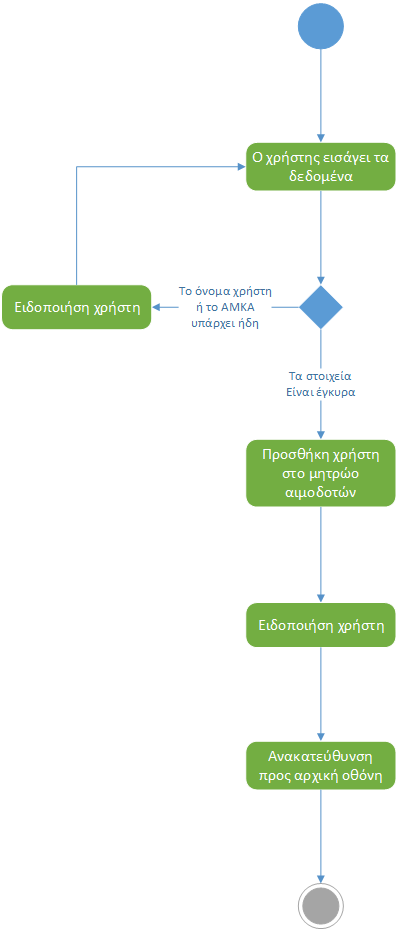
\includegraphics[width=0.7\textwidth]{Register.png}
		    \caption{Ακολουθιακό διάγραμμα \#1. Εγγραφή εθελοντή αιμοδότη στο σύστημα.}
		    \label{fig:register}
		\end{figure}
		
		
		\begin{figure}[H]
		    \centering
		    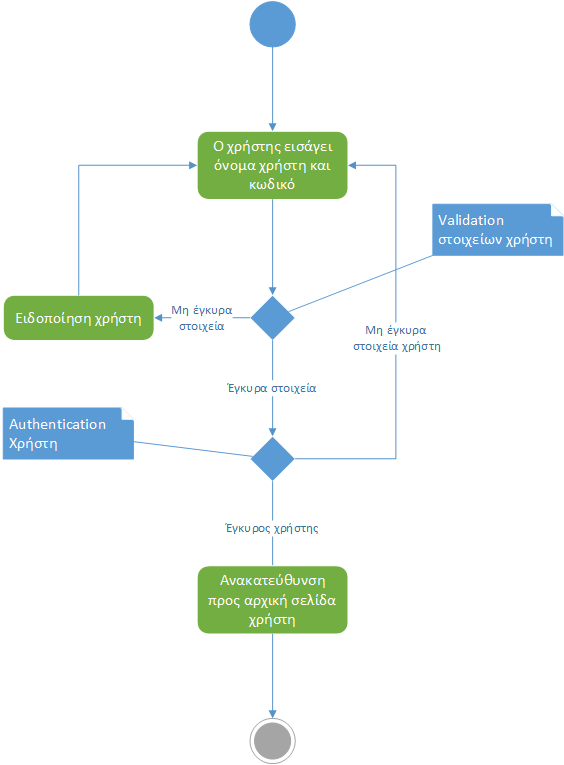
\includegraphics[width=1\textwidth]{Login.png}
		    \caption{Ακολουθιακό διάγραμμα \#2. Είσοδος εθελοντή αιμοδότη στο σύστημα.}
		    \label{fig:login}
		\end{figure}
		
		\begin{figure}[H]
		    \centering
		    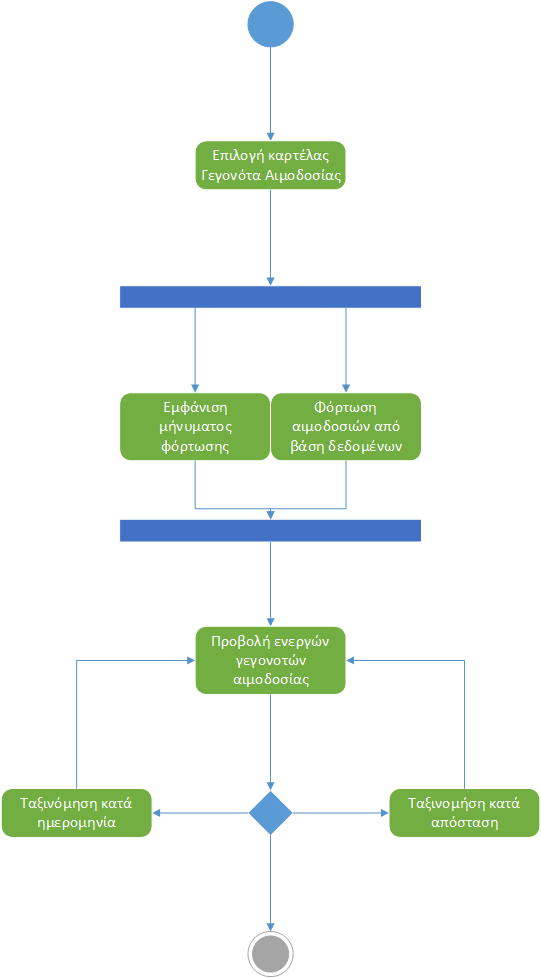
\includegraphics[width=0.7\textwidth]{ViewDonationEvents.png}
		    \caption{Ακολουθιακό διάγραμμα \#3. Προβολή γεγονότων αιμοδοσίας, από τον εθελοντή αιμοδότη.}
		    \label{fig:view}
		\end{figure}
		
	    \begin{figure}[H]
		    \centering
		    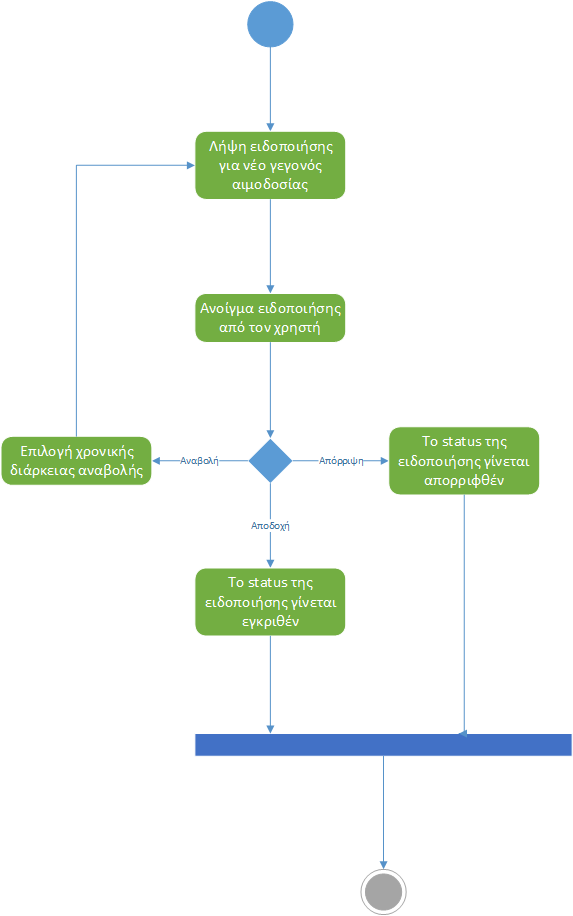
\includegraphics[width=0.9\textwidth]{ManageNotifications.png}
		    \caption{Ακολουθιακό διάγραμμα \#4. Διαχείριση των ειδοποιήσεων για τα γεγονότα αιμοδοσίας από τον εθελοντή αιμοδότη.}
		    \label{fig:manage}
		\end{figure}

		
		\begin{figure}[H]
		    \centering
		    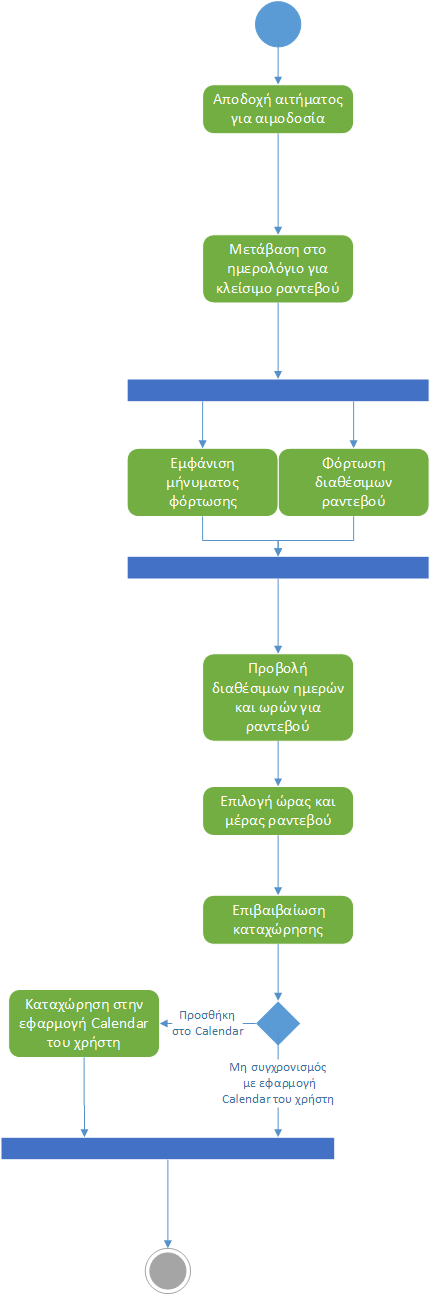
\includegraphics[width=0.5\textwidth]{CreateReservation.png}
		    \caption{Ακολουθιακό διάγραμμα \#5. Κλείσιμο ραντεβού για αιμοδοσία από τον εθελοντή αιμοδότη.}
		    \label{fig:createAppoint}
		\end{figure}
		
				
		\begin{figure}[H]
		    \centering
		    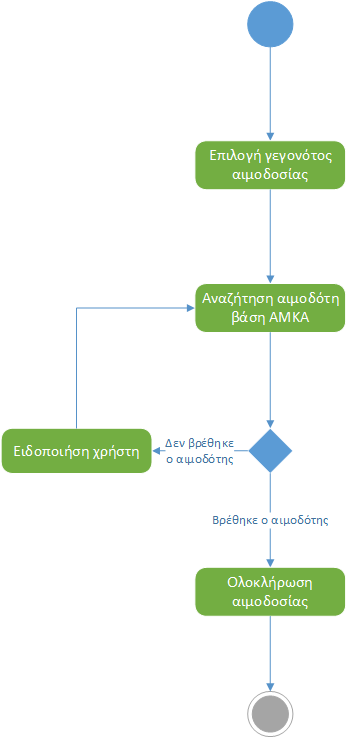
\includegraphics[width=0.7\textwidth]{CompleteDonation.png}
		    \caption{Ακολουθιακό διάγραμμα \#6. Καταχώρηση αιμοδοσίας από τον  εγκεκριμένο χρήστη/διαχειριστή του συστήματος αιμοδοσίας σύστημα.}
		    \label{fig:complete}
		\end{figure}
		
	    \begin{figure}[H]
		    \centering
		    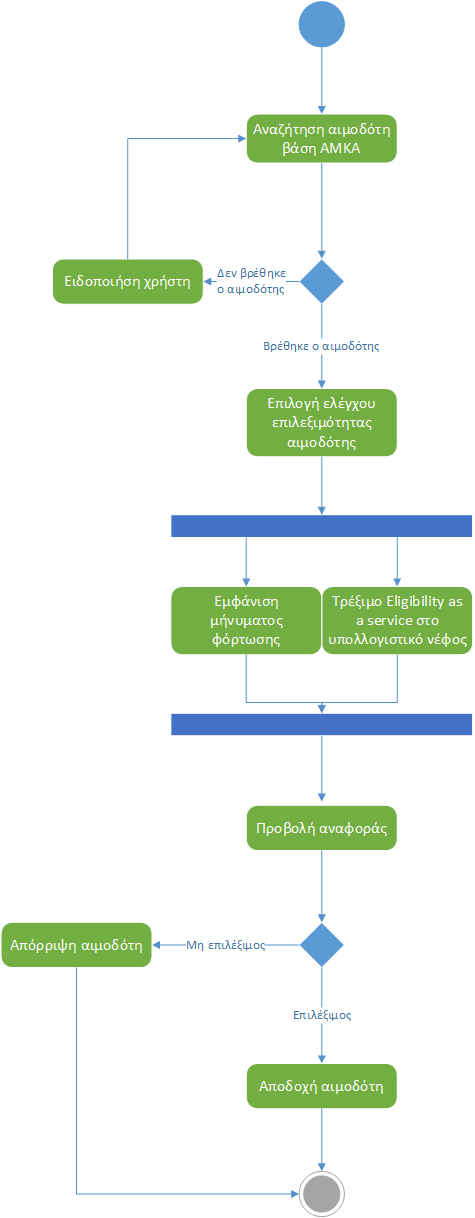
\includegraphics[width=0.55\textwidth]{EligibilityTest.png}
		    \caption{Ακολουθιακό διάγραμμα \#7. Έλεγχος καταλληλότητας του υποψήφιου αιμοδότη από τον  εγκεκριμένο χρήστη/διαχειριστή του συστήματος αιμοδοσίας.}
		    \label{fig:eligibiity}
		\end{figure}
		
\section{Business Model}
	\subsection{Gamification}
	
		Το gamification (παιχνιδοποιήση) ορίζεται ως ``η ενσωμάτωση διάφορων πρακτικών και διαδικασιών παιχνιδιού σε καταστάσεις που δεν σχετίζονται με το παιχνίδι με στόχο τη λύση προβλημάτων μέσω της αύξησης της διαδραστικότητας και της συμμετοχής των χρηστών"\cite{Deterding:2011:GDE:2181037.2181040}\cite{Rojas:2013:MPG:2583008.2583033}. Ως εκ τούτου, το gamification έχει βρει χρήση σε ένα ευρύ φάσμα εφαρμογών, από τον χώρο του marketing και της εκπαίδευσης μέχρι και τον χώρο της υγείας \cite{6758978}. Το Gartner έχει εκτιμήσει ότι μέχρι το τέλος του 2015 περισσότερο από το 50\% των επιχειρήσεων θα αξιοποιεί το gamification \cite{gartnerGamification}. Στον ακαδημαϊκό χώρο συναντάμε όλο και περισσότερη έρευνα και δημοσιεύσεις με στόχο να μελετηθεί με μετρήσιμα, αντικειμενικά κριτήρια κατά πόσο είναι αποτελεσματική η χρήση των τεχνικών gamification. 

	\subsubsection{Δομικά στοιχεία}
	Ένα παιχνίδι αποτελείται από έξι δομικά στοιχεία, όπως παρουσιάζονται στο σχήμα \ref{fig:gamification_components}.
		
		\begin{figure}[h]
		    \centering
		    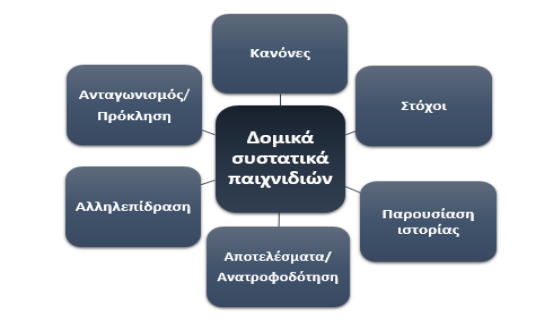
\includegraphics[width=0.7\textwidth]{gamification_components.jpg}
		    \caption{Δομικά στοιχεία παιχνιδιών}
		    \label{fig:gamification_components}
		\end{figure}
	
		Ένας από τους βασικούς στόχους ενός συστήματος gamification αποτελεί η αύξηση της ενασχόλησης του χρήστη. Τα στάδια με τα οποία ευελπιστεί να το πετύχει έχουν ως εξής:
		\begin{enumerate}
			\item Κίνητρα: Στην αρχή της διαδικασίας θα πρέπει να δοθεί στον χρήστη κάποιο κίνητρο το οποίο διαφέρει ανάλογα με τον τύπο χρήστη καθώς και τους στόχους του συστήματος. Παράδειγμα ενός τέτοιου κινήτρου αποτελεί η κοινωνική αναγνώριση \cite{Gamification_on_Participation}.
			\item Ενέργειες: είναι το δεύτερο στάδιο στο οποίο ο χρήστης οδηγείται μέσω των κινήτρων του πρώτου σταδίου. Σε αυτό το στάδιο ο χρήστης πραγματοποιεί την επιθυμητή από το σύστημα ενέργεια. Για παράδειγμα σε μια εφαρμογή εκμάθησης ξένων γλωσσών μια ενέργεια μπορεί να είναι η επανάληψη του λεξιλογίου.
			\item Επιβραβεύσεις: Ύστερα από την επιτυχή ολοκλήρωσης της ενέργειας ή των ενεργειών στο δεύτερο βήμα ο χρήστης λαμβάνει κάποια μορφή επιβράβευσης. Παραδείγματα επιβραβεύσεων που βρίσκουν ευρεία χρήση στο gamification αποτελούν τα εικονικά νομίσματα και τα εικονικά αγαθά.
			\item Κατορθώματα: Στο τελευταίο αυτό στάδιο ο χρήστης φτάνει σε κάποιο κατόρθωμα το οποίο ενισχύει τα κίνητρα του και ο κύκλος επαναλαμβάνεται \cite{GamificationDesign}.
		\end{enumerate}
		Η διαδικασία όπως την περιγράψαμε εμφανίζεται στο σχήμα \ref{fig:engagement_loop}.
		\begin{figure}[h]
		    \centering
		    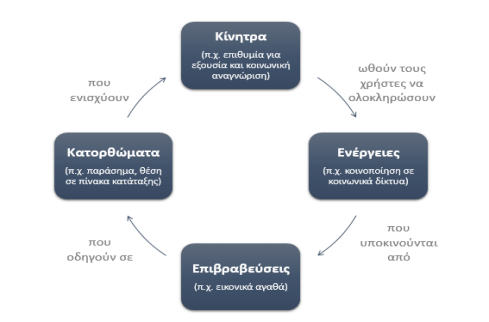
\includegraphics[width=0.7\textwidth]{engagement_loop.jpg}
		    \caption{Κύκλος ενασχόλησης}
		    \label{fig:engagement_loop}
		\end{figure}

	
	\subsubsection{Σχεδιασμός συστήματος}	
		Κατά τον σχεδιασμό του συστήματος gamification ακολουθήσαμε το πλαίσιο ΜΔΑ (MDA), το οποίο προέρχεται από τα αρχικά των λέξεων Μηχανισμοί (Mechanics), Δυναμικές (Dynamics) και Αισθητικά στοιχεία (Aesthetics) \cite{citeulike:382810}. Σύμφωνα με το προαναφερθέν πλαίσιο τα βασικά στοιχεία που απαρτίζουν ένα παιχνίδι είναι οι κανόνες το σύστημα και η διασκέδαση όπως φαίνεται και στο σχήμα \ref{fig:mda_1}.
	
		\begin{figure}[h]
		    \centering
		    
\includegraphics[width=0.7\textwidth]{mda_1.jpg}
		    \caption{Στοιχεία παιχνιδιού}
		    \label{fig:mda_1}
		\end{figure}	
	
		Ενώ για το κομμάτι του σχεδιασμού έχουμε το σχήμα \ref{fig:mda_2}:	
	
		\begin{figure}[h]
		    \centering
		    
\includegraphics[width=0.7\textwidth]{mda_2.jpg}
		    \caption{Πλαίσιο σχεδίασης}
		    \label{fig:mda_2}
		\end{figure}
	
		Πριν προχωρήσουμε στην ανάλυση και παρουσίαση των σχεδιαστικών αποφάσεων που πήραμε, με σκοπό να γίνουν καλύτερα κατανοητές, κρίνουμε σκόπιμο να αναλύσουμε τις παραπάνω έννοιες δεδομένου ότι αποτελεί πολύ συχνό φαινόμενο η ύπαρξη σύγχυσης μεταξύ των εννοιών μηχανισμοί και δυναμικές.
		\begin{itemize}
		
			\item \textbf{Μηχανισμοί:} περιγραφούν συγκεκριμένα δομικά στοιχεία του παιχνιδιού σε επίπεδο αναπαράστασης δεδομένων και αλγορίθμων. Συνδυάζοντας διάφορους βασικούς μηχανισμούς μπορούμε να κατασκευάσουμε πιο πολύπλοκες δομές οι οποίες μπορούν να φέρουν το επιθυμητό αποτέλεσμα. Οι μηχανισμοί είναι αυτοί που υποστηρίζουν τις δυναμικές.
			
			\item \textbf{Δυναμικές:} περιγράφουν πως οι κανόνες του παιχνιδιού αλληλεπιδρούν με τον χρήστη και τους μηχανισμούς. Σε προγραμματιστική ορολογία μπορεί να περιγραφεί ως η συμπεριφορά του παιχνιδιού κατά την διάρκεια εκτέλεσης του. Ρόλος των δυναμικών είναι να κάνουν το παιχνίδι προοδευτικά δυσκολότερο αποφεύγοντας την ρουτίνα και διατηρώντας αμείωτο το ενδιαφέρων του χρήστη.
			\item \textbf{Αισθητικά στοιχεία:} περιγράφουν τα συναισθήματα που επιδιώκει το σύστημα να προξενήσει στον χρήστη του. Σύμφωνα με τους δημιουργούς του προτύπου MDA κάποια από αυτά είναι:
			
			\begin{itemize}
				\item Αίσθηση ( Το παιχνίδι παρουσιάζεται σαν εσωτερική ευχαρίστηση).
				\item Φαντασία (Το παιχνίδι σαν ιστορία με σκοπό να ταξιδέψει τον παίχτη μακριά από την πραγματικότητα).
				\item Αφήγηση (Το παιχνίδι ως ιστορία με πλοκή).
				\item Πρόκληση (Ο παίκτης πρέπει να ξεπεράσει κάποια εμπόδια).
				\item Συνεργασία (Το παιχνίδι με την κοινωνική του υπόσταση).
				\item Ανακάλυψη (Το παιχνίδι με κέντρο την ανακάλυψη του καινούριου).
				\item Έκφραση (Το παιχνίδι ως εξερεύνηση του εαυτού).
				\item Υποβολή (Το παιχνίδι ως απλό μέσο για αναψυχή κατά τον ελέυθερο χρόνο
	του ατόμου).
	
			\end{itemize}
		\end{itemize}
		
		Κατά τον σχεδιασμό ενός συστήματος gamification, λαμβάνοντας υπόψιν τους στόχους του συστήματος γίνεται διαφορετικός συνδυασμός των παραπάνω στοιχείων. Οι πιο συχνά χρησιμοποιούμενοι μηχανισμοί είναι οι πόντοι, οι πίνακες κατάταξης καθώς και τα παράσημα. Στον πίνακα \ref{tab:gamifaction_mechanisms} βλέπουμε διάφορους μηχανισμούς καθώς και τους στόχους που θέλουν να πετύχουν \cite{raey}\cite{Lucassen2014194}.
	
	\begin{table}[H]
		\begin{center}
		    \begin{tabular}{|c|l|}
		    \hline
		    \rowcolor{grayy}
		    \textbf{Στόχος} & \textbf{Μηχανισμός}
		    \\ \hline    
		    \multirow{12}{*}{\textbf{Ενασχόληση}} & Πίνακες Κατάταξης \\ & Επίπεδα \\ & Εικονικές επιβραβεύσεις προσπάθειας \\ & Ανταγωνισμός \\ & Αίσθηση συμμετοχής σε ομάδα \\ &  Έλεγχος σε συμπαίκτες \\ &  Διαφοροποίηση από συμπαίκτες \\ & Βοήθεια σε φίλο \\ & Χρονικοί περιορισμοί \\ & Λήξη χρόνου \\ & Περιορισμοί σε πόρους \\ \hline
		    \multirow{3}{*}{\textbf{Αφοσίωση}}  & Περιορισμοί σε πρόσβαση \\ & Παράσημα \\ & Εικονικές επιβραβεύσεις \\ \hline
		    \multirow{3}{*}{\textbf{Επίγνωση}}  & Προωθήσεις \\ & Λοταρίες  \\ \hline
		    \end{tabular}
		    \caption{Στόχοι και μηχανισμοί του Gamification}
			\label{tab:gamifaction_mechanisms}
		\end{center}
	\end{table}

		Για να γίνει ξεκάθαρος ο διαχωρισμός μεταξύ δυναμικών και μηχανισμών στον πίνακα \ref{tab:gamifaction_dynamics} παρουσιάζουμε τους μηχανισμούς ενός παιχνιδιού με τις αντίστοιχες δυναμικές και κίνητρα \cite{BlohmIvo2013}.
	
	\begin{table}[H]
		\begin{center}
		    \begin{tabular}{|l|l|l|}
		    \hline
		    \rowcolor{grayy}
		    \textbf{Μηχανισμοί} & \textbf{Δυναμικές} & \textbf{Κίνητρα}
		    \\ \hline
		     Καταγραφή συμπεριφοράς & Εξερεύνηση & Περιέργεια   
		     \\ \hline
		     Συστήματα πόντων, εμβλήματα και επιβραβεύσεις & Συλλογή (εικονικών αγαθών) & Κατόρθωμα
		     \\ \hline
		     Κατάταξη, επίπεδα & Ανταγωνισμός & Κοινωνική αναγνώριση
		     \\ \hline
		     Ομαδικές δραστηριότητες & Συνεργασία & Επικοινωνία
		     \\ \hline
		     Πίεση χρόνου, χρονική περιορισμοί & Πρόκληση & Διέγερση
		     \\ \hline
		     Εικονικοί χαρακτήρες και κόσμοι & Ανάπτυξη, Οργάνωση & Αυτοδιάθεση
		     \\ \hline
		    \end{tabular}
		    \caption{Μηχανισμοί, δυναμικές και κίνητρα στο Gamification}
			\label{tab:gamifaction_dynamics}
		\end{center}
	\end{table}
	
	\subsubsection{Gamification στο σύστημα μας}
		Έχοντας παρουσιάσει το θεωρητικό πλαίσιο του gamification, στην συνέχεια παρουσιάζουμε την χρήση του στο σύστημα που αναπτύξαμε στο πλαίσιο της παρούσας διπλωματικής. Μέσω του gamification επιδιώκουμε να πετύχουμε κυρίως τους δύο πρώτους στόχους της διπλωματικής όπως περιγράφηκαν στην ενότητα \ref{sec:intro_goals}.
		
	\subsubsection{Σύστημα επιβραβεύσεων}
	Οι επιβραβεύσεις δίνονται στον εθελοντή αιμοδότη (χρήστη του συστήματος) ανάλογα με την δραστηριότητα του και τους πόντους που έχει συγκεντρώσει. Οι επιβραβεύσεις μπορούν να χωριστούν σε δύο μεγάλες κατηγορίες:
	\begin{itemize}
		\item \textbf{Φυσικές Επιβραβεύσεις:} Ο χρήστης θα μπορεί να εξαργυρώνει τους πόντους που έχει μαζέψει για να κερδίσει υπηρεσίες ή προϊόντα από συνεργαζόμενες υπηρεσίες που τα έχουν διαθέσει τα πλαίσια κοινωνικής ευθύνης. Για παράδειγμα αν υπάρξει κάποια συνεργασία με την Cosmote μια μορφή φυσικής επιβράβευσης θα μπορούσε να είναι επιπλέον χρόνος ομιλίας.
		 \item \textbf{Εικονικές Επιβραβεύσεις:} Η μορφή των εικονικών επιβραβεύσεων που χρησιμοποιήσαμε στο σύστημα μας είναι τα εμβλήματα, τα οποία ο χρήστης θα λαμβάνει για διάφορες δραστηριότητες που επιτελεί. Συγκεκριμένα ο χρήστης κερδίζει εμβλήματα όταν:
		 
		 	\begin{itemize}
		 		\item Εγγράφεται στο σύστημα ως εθελοντής αιμοδότης
		 		\item Πραγματοποιεί την πρώτη του αιμοδοσία
		 		\item Συμπληρώνει τον μέγιστο αριθμό αιμοδοσιών που επιτρέπεται σε κάποιο ημερολογιακό έτος
		 		\item Καλεί κάποιον φίλο του να χρησιμοποιήσει την εφαρμογή
		 		\item Ανταποκρίνεται σε αιτήματα για αιμοδοσίες
		 	\end{itemize}
		 	Η παραπάνω λίστα είναι καθαρά ενδεικτική, δεδομένου ότι η δημιουργία εμβλημάτων αποτελεί μια δυναμική διαδικασία που έχει σκοπό να κρατήσει αμείωτο το ενδιαφέρον του εθελοντή. Για παράδειγμα ο διαχειριστής του συστήματος θα μπορεί να δημιουργεί ειδικά εμβλήματα για ένα συγκεκριμένο γεγονός αιμοδοσίας το οποίο έχει συγκεκριμένη ημερομηνία.
	\end{itemize}
	
	Σε αυτό το σημείο θα πρέπει να αναφέρουμε ότι, έχει αποτελέσει αντικείμενο τεράστιας διαμάχης το κατά πόσο πρέπει να δίνονται φυσικές επιβραβεύσεις στους εθελοντές και κατά πόσο αυτό αφαιρεί το νόημα της εθελοντικής αιμοδοσίας. Στην Ελλάδα μέχρι πρωτινός δεν επιτρεπόντουσαν κίνητρα που θα μπορούσαν να θεωρηθούν αντικαταστατό του χρήματος, αλλά ο πρόσφατος νόμος 4272/2014 άρθρο 27 δίνει την ελευθερία στον Ε.ΚΕ.Α. να ορίσει τέτοιου είδους κίνητρα σε συμφωνία με την οδηγία 2002/98 της Ευρωπαϊκής ένωσης.
	
	\subsubsection{Σύστημα πόντων}\label{sssect:point_system}
	
	Το σύστημα gamification που εφαρμόζουμε στην εφαρμογή που αναπτύχθηκε στα πλαίσια της παρούσας διπλωματικής περιλαμβάνει ολοκληρωμένο σύστημα πόντων. Ο χρήστης με το που εγγράφεται στο σύστημα λαμβάνει έναν μικρό αριθμό πόντων ως επιβράβευση της εγγραφής του ως εθελοντής αιμοδότης. Οι πόντοι μπορούν αν χωριστούν σε δύο επιμέρους κατηγορίες βάση της χρήσης τους:

	\begin{itemize}
		\item \textbf{Πόντοι εξαργύρωσης:} εξαργυρώνονται με σκοπό της απόκτησης κάποιας επιβράβευσης. Ανάλογα με τις δραστηριότητες που επιτελεί κερδίζει πόντους οι οποίοι αθροίζονται. Ενδεικτική λίστα για τις οποίες ο χρήστης θα μπορεί να κερδίζει πόντους:
		\begin{itemize}
			\item Εγγραφή στο σύστημα.
			\item Πραγματοποίηση αιμοδοσίας.
			\item Πρόσκληση φίλων στην εφαρμογή.
			\item Αλληλεπίδραση με τα κοινωνικά δίκτυα.
		\end{itemize}
		\item \textbf{Πόντοι εμπειρίας:} ουσιαστικά είναι οι συνολικοί πόντοι που έχει αποκτήσει ο εθελοντής από την έναρξη χρήσης της εφαρμογής. Οι πόντοι εμπειρίας χρησιμοποιούνται για τον πίνακα κατάταξης μεταξύ των ``φίλων" του, καθώς και για τον συνολικό πίνακα κατάταξης.
	\end{itemize}
	Κρίνεται σκόπιμο να αναφερθεί ότι οι πόντοι κατανέμονται με βάση την βαρύτητα της δραστηριότητας που εκτελεί ο εθελοντής αιμοδότης.
	
	\subsubsection{Πίνακες κατάταξης}
	
	Οι πίνακες κατάταξης δείχνουν την επίδοση και την `πρόοδο' ενός χρήστη σε σχέση με αυτή των `φίλων' τους \cite{Liu:2011:GIE:2072652.2072655}. Υπάρχει ένας ενιαίος πίνακας στον οποίο και θα υπάρχουν όλοι οι εθελοντές που χρησιμοποιούν το σύστημα, εφόσον έχουν δηλώσει ότι επιθυμούν να συμμετέχουν στην κατάταξη. Ενώ υπάρχει και ένας δεύτερος πίνακας που δημιουργείται δυναμικά για κάθε χρήστη και περιλαμβάνει μόνο άτομα τα οποία ακολουθεί. Η κατάταξη διαμορφώνεται με βάση τους πόντους εμπειρίας που έχει μαζέψει κάθε χρήστης, οι οποίοι περιγράφηκαν παραπάνω. Για τους πρώτους στον κεντρικό πίνακα κατάταξης θα υπάρχει μέριμνα για κάποια ειδική επιβράβευση, ανάλογα τις συμφωνίες και χορηγίες που υπάρχουν με εταιρείες στα πλαίσια της κοινωνικής ευθύνης.
	
	\subsubsection{Συμπέρασμα}
	
	Συμπερασματικά το σύστημα που περιγράψαμε παραπάνω μπορεί να βοηθήσει σημαντικά στον δεύτερο στόχο που θέσαμε στην εισαγωγή της διπλωματικής, στην ενότητα \ref{sec:intro_goals}, δηλαδή στη διατήρηση και επιπλέον ενεργοποίηση των εθελοντών αιμοδοτών. Για την επίτευξη του πρώτου στόχου που θέσαμε δηλαδή τη στρατολόγηση περισσότερων νέων εθελοντών θεωρούμε πως μεγάλο ρόλο μπορεί να παίξει ο συνδυασμός του gamification με τα κοινωνικά δίκτυα όπως περιγράφουμε στην επόμενη ενότητα.
	
	\subsection{Social Networking Integration}\label{ssec:social_netowrks_system_analysis}

	Η θεωρία της κοινωνικοποίησης των καταναλωτών προβλέπει ότι η επικοινωνία μεταξύ των καταναλωτών επηρεάζει τη γνωστική και συναισθηματική τους συμπεριφορά, καθώς και τις στάσεις τους απέναντι σε ένα προϊόν ή μια υπηρεσία\cite{1974}. Τα κοινωνικά δίκτυα μπορούν να επηρεάσουν δραστικά την συμπεριφορά ενός ατόμου\cite{shaver2007impact} και οι υπάρχοντες εθελοντές μέσω των κοινωνικών δικτύων, είναι σε θέση να παίξουν τον ρόλο του πρέσβη προσελκύοντας νέους εθελοντές αιμοδότες. Η αξιοποίηση των εθελοντών με στόχο την προαγωγή της εθελοντικής αιμοδοσίας, αποτελεί μια εξαιρετικά αποτελεσματική μέθοδο "στρατολόγησης" και αύξησης του αριθμού των αιμοδοσιών \cite{Lemmens2008}. Πριν προχωρήσουμε στην ανάλυση των συγκεκριμένων ενεργειών που επιτελέσαμε με αυτό τον σκοπό, κρίνουμε σκόπιμο να αναφέρουμε μερικές εισαγωγικές έννοιες για τα κοινωνικά δίκτυα εν γένει. 	
	
	Τα μέσα κοινωνικής δικτύωσης (Social Media), μέσω των οποίων επιτυγχάνεται η ηλεκτρονική κοινωνική δικτύωση, αποτελούν ουσιαστικά απόρροια του Web 2.0, το οποίο κατάφερε να αλλάξει την υφή του διαδικτύου προσδίδοντάς του μια πιο κοινωνική διάσταση. Ο όρος κοινωνικά δίκτυα (social media), αποτελεί μια γενική έννοια που χρησιμοποιείται για να περιγράψει διαδικτυακές εφαρμογές και υπηρεσίες στις οποίες οι χρήστες έχουν την δυνατότητα να δημιουργήσουν και να μοιραστούν μεταξύ τους περιεχόμενο \cite{Kaplan201059}. Τα μέσα κοινωνικής δικτύωσης μπορούν να χωριστούν σε έξι κατηγορίες με βάση τον βαθμό της κοινωνικής παρουσίας που απαιτούν από τον χρήστη:
	\begin{itemize}
		\item Ιστολόγια (π.χ Blogger, Tumblr, Wordpress)
		\item Συνεργατικές ιστοσελίδες - έργα (π.χ Wikipedia)
		\item Ιστοσελίδες κοινωνικής δικτύωσης (π.χ Facebook)
		\item Κοινότητες διαμοιρασμού περιεχομένου (π.χ Reddit, Youtube)
		\item Εικονικοί κόσμοι (π.χ Second Life)
		\item Εικονικοί κόσμοι παιχνιδιών (π.χ World of Warcraft)
	\end{itemize}
	
	Τα μέσα κοινωνικής δικτύωσης βρήκαν τέτοια ευρεία αποδοχή και εδραιώθηκαν στην καθημερινότητα μας γιατί ικανοποιούν μια ισχυρή ανάγκη του ανθρώπου. Την ανάγκη του να συνεταιρίζεται, δημιουργώντας δίκτυα με άλλους ανθρώπους, ανταλλάζοντας ιδέες και απόψεις. Τα κύρια κίνητρα για τη χρήση των μέσων κοινωνικής δικτύωσης είναι τα εξής \cite{Benkler2006}:
	\begin{itemize}
		\item Κοινωνικοποίηση
		\item Ψυχική ευεξία
		\item Ατομική ικανοποίηση
		\item Κοινωνική αναγνώριση
	\end{itemize}		
	
	Όπως αναφέραμε και παραπάνω ο κύκλος της ενασχόλησης (σχήμα \ref{fig:engagement_loop}) ξεκινάει από το κίνητρο. Ένα από τα βασικότερα κίνητρα του ανθρώπου είναι η επιθυμία για κοινωνική αναγνώριση και προβολή \cite{Gamification_on_Participation} την οποία πολλές φορές επιδιώκει να ικανοποιήσει μέσω των κοινωνικών δικτύων (όπως φαίνεται από την παραπάνω λίστα).
	
	Η εφαρμογή που αναπτύξαμε στα πλαίσια της διπλωματικής εργασίας δίνει την δυνατότητα στον εθελοντή (χρήστη) να μοιραστεί στα κοινωνικά δίκτυα τα επιτεύγματα του καθώς και πληροφορίες σε κάθε στάδιο της αιμοδοσίας, ικανοποιώντας με αυτό τον τρόπο το αίσθημα της κοινωνικής αναγνώρισης. Συγκεκριμένα υπάρχει άμεση διασύνδεση με το facebook και το twitter στα οποία ο χρήστης ενθαρρύνεται να δημοσιεύσει στις παρακάτω περιπτώσεις:
	\begin{itemize}
		\item Όταν λαμβάνει ειδοποίηση για γεγονός αιμοδοσίας, του δίνεται η δυνατότητα να το μοιραστεί στα μέσα κοινωνικής δικτύωσης. Με αυτό τον τρόπο αυξάνεται η προβολή του γεγονότος αιμοδοσίας και κατ' επέκταση οι πιθανότητες να καλυφθούν οι ανάγκες σε αίμα που έχουν τεθεί, ενώ προβάλλεται και η ίδια η εφαρμογή το οποίο οδηγεί στην στρατολόγηση περισσότερων εθελοντών αιμοδοτών.
		\item Όταν ολοκληρώνει κάποια αιμοδοσία ο χρήστης παροτρύνεται να βγάλει φωτογραφία και να τη μοιραστεί στα μέσα κοινωνικής δικτύωσης, προάγοντας την αιμοδοσία.
		\item Όταν ξεκλειδώνει κάποιο έμβλημα.
	\end{itemize}
	
	Επίσης ο χρήστης έχει τη δυνατότητα να προσκαλέσει τους φίλους του στην εφαρμογή. Σε αυτό το σημείο πρέπει να αναφερθεί ότι κάθε φορά που ο χρήστης αλληλεπιδρά μέσω της εφαρμογής με τα μέσα κοινωνικής δικτύωσης κερδίζει πόντους σύμφωνα με το σύστημα πόντων όπως περιγράφηκε στο \ref{sssect:point_system} . Αξιοποιώντας τη δύναμη των κοινωνικών δικτύων είμαστε σε θέση να δώσουμε μεγαλύτερη προβολή και κοινωνικό χαρακτήρα στην εθελοντική αιμοδοσία. Μετατρέποντας ουσιαστικά τους εθελοντές αιμοδότες σε πρότυπα της εθελοντικής αιμοδοσίας με στόχο την προσέλκυση νέων εθελοντών αιμοδοτών.
	
	\subsection{Ειδοποιήσεις και Υπενθυμίσεις}
		
		 Όταν υπάρχει κάποια συγκεκριμένη ανάγκη για αίμα ή ένα καθορισμένο γεγονός αιμοδοσίας, το σύστημα στέλνει στους εθελοντές αιμοδότες νέες ειδοποιήσεις (push notifications). Οι ειδοποιήσεις αυτές δεν αποστέλλονται σε όλους τους χρήστες που είναι εγγεγραμμένοι στην εφαρμογή, αντιθέτως το σύστημα τρέχει κάποιους ``έξυπνους αλγορίθμους" και επιλέγει την ομάδα χρηστών που τηρούν τις απαραίτητες προϋποθέσεις. Τα κριτήρια που ελέγχει το σύστημα αφορούν στο αν έχει παρέλθει το απαιτούμενο διάστημα μέχρι να μπορεί να δώσει ξανά αίμα ο εθελοντής, στην καταλληλότητα με βάση τη γεωγραφική του τοποθεσία και στο αν έχει τη ζητούμενη ομάδα αίματος, στην περίπτωση που υπάρχουν .
		 
		
		Ο χρήστης έχει την επιλογή να αποδεχθεί, να απορρίψει και να αναβάλει την ειδοποίηση. Στην περίπτωση αποδοχής, ο χρήστης μπορεί να κλείσει ένα ραντεβού με το αντίστοιχο κέντρο αιμοδοσίας καθώς το σύστημα παρέχει ολοκληρωμένη διαχείριση ραντεβού. Η εφαρμογή έχει τη δυνατότητα να παρέχει υπενθυμίσεις εγκαίρως μέσα από πολλούς διαφορετικούς τρόπους, όπως μήνυμα ηλεκτρονικού ταχυδρομείου, επαναποστολή της ειδοποίησης και συγχρονισμός και καταχώρηση στο ημερολόγιο του χρήστη). Σε περίπτωση που ο χρήστης απορρίψει ένα αίτημα, αυτό μεταφέρεται και εμφανίζεται αυτόματα στο ιστορικό των χρηστών, στην ενότητα των απορριφθέντων αιτημάτων. Ως εκ τούτου ο χρήστης μπορεί να αναθεωρήσει τα αιτήματα του και να το εξετάσει σε μεταγενέστερο χρόνο. 
		
		 Σύμφωνα με μελέτες που έχουν γίνει υπάρχει μεγάλος αριθμός αιμοδοτών που ενώ πληρούν τις απαραίτητες προϋποθέσεις και έχουν την θέληση να αιμοδοτήσουν, δεν προβαίνουν σε αιμοδοσία επειδή δεν υπάρχει κάποιος να τους το υπενθυμίσει \cite{Marantidou2007}. Η αντιμετώπιση αυτού του προβλήματος επιτυγχάνεται με τις συστηματικές ειδοποιήσεις που λαμβάνει ο αιμοδότης, οι οποίες εκτός από μέσο για υπενθύμιση, δρουν ως κινητήριος δύναμη αφύπνισης και διατήρησης της εθελοντικής συνείδησης του αιμοδότη.
		 
		 Ένα άλλο φαινόμενο το οποίο δυσχεραίνει ακόμα περισσότερο την ήδη δύσκολη κατάσταση στον τομέα των αιμοδοσιών είναι η προσωρινή απόρριψη των αιμοδοτών.  Το φαινόμενο αυτό  λαμβάνει χώρα σε περιπτώσεις που οι χρήστες αποκλείονται προσωρινά από την αιμοδοσία, λόγω του ότι δεν τηρούν τα κριτήρια ακαταλληλότητας (π.χ. πήραν ασπιρίνη την ημέρα της αιμοδοσίας). Από τον συνολικό αριθμό αιμοδοσιών το 14.13\% αποκλείονται για λόγους προσωρινής ακαταλληλότητας \cite{WorldHealth}. Μελέτες έχουν δείξει ότι οι περισσότεροι εθελοντές δεν επιστρέφουν αν απορριφθούν μία φορά, συγκεκριμένα μόλις το 11\% επιστρέφει μετά την απαιτούμενη περίοδο για να πραγματοποιήσει δωρεά αίματος \cite{halperin1998effect}. Όταν τηρούνται οι κατάλληλες συνθήκες ώστε να είναι σε θέση ο αιμοδότης να προσφέρει πάλι αίμα, η εφαρμογή του στέλνει ειδοποιήσεις για τα γεγονότα αιμοδοσίας ώστε να τον παρακινήσει και να του υπενθυμίσει να δώσει αίμα.
		 
	
		 Με βάση τα όσα προαναφέρθηκαν, η χρήση κατάλληλων ειδοποιήσεων και ως προς την χρονική συχνότητα και ως το προς τον παραλήπτη τους, βοηθάει στην τακτική συμμετοχή των εθελοντών σε αιμοδοσίες και συντελεί στην αντιμετώπιση κάποιων από τα προβλήματα που τους αποθαρρύνουν. Η σωστή διαχείριση και αποστολή των ειδοποιήσεων είναι ένα πολύ σημαντικό ζήτημα, καθώς δεν πρέπει να στέλνονται περιττές ή λανθασμένα επαναλαμβανόμενες ειδοποιήσεις, οι οποίες μπορεί να έχουν ως αποτέλεσμα να κουράσουν τον χρήστη αλλά πρέπει η συχνότητα αποστολής τους να αποφέρει το βέλτιστο αποτέλεσμα. Στόχος του συστήματος ειδοποιήσεων είναι η ανταπόκριση να αυξηθεί με ικανοποιητικό ρυθμό και οι αιμοδοσίες να πολλαπλασιαστούν\cite{Marantidou2007}.
	
	
	\subsection{Heamovigilance}
	
		Ένα άλλο θέμα για το οποίο λαμβάνεται μέριμνα είναι το ζήτημα της αιμοεπαγρυπνήσης. Μία απαραίτητη προϋπόθεση για την αποτελεσματική εφαρμογή της αιμοεπαγρυπνήσης είναι η ύπαρξη συστήματος ιχνηλασιμότητας, δηλαδή πρέπει να εξασφαλίζεται η ικανότητα εντοπισμού καθεμίας από τις μονάδας αίματος ή καθενός από τα παράγωγα προϊόντα αίματος που προέρχονται από αυτήν, από τον εθελοντή αιμοδότη μέχρι τον τελικό προορισμό τους.
		
		
		Το σύστημα μας, αρχικά καταγράφει τον αιμοδότη από τον οποίο προήλθε το αίμα. Στην συνέχεια, κάθε μονάδα αίματος παρακολουθείται με χρήση RFIDs και όταν τελικά φτάσει στον τελικό αποδέκτη το πληροφοριακό σύστημα του νοσοκομείου αποθηκεύει την πληροφορία αυτή στο πληροφοριακό του σύστημα. Με χρήση κατάλληλων πρωτοκόλλων και ασφαλούς διαύλου επικοινωνίας το σύστημα μας λαμβάνει από το πληροφοριακό σύστημα του νοσοκομείου το όνομα και το μοναδικό αναγνωριστικό του ασθενούς (ΑΜΚΑ) και τα αποθηκεύει, συσχετίζοντας τα με τα στοιχεία του αιμοδότη. Αυτή η διαδικασία έχει ως αποτέλεσμα να κρατείται πλήρες ηλεκτρονικό αρχείο το οποίο συσχετίζει σε περιπτώσεις ανεπιθύμητων συμβαμάτων τον αιμοδότη με τον αιμολήπτη. Η λειτουργία είναι ιδιαίτερα σημαντική για την ελαχιστοποίηση των ανεπιθύμητων κρουσμάτων και κατ 'επέκταση για τη δημόσια υγεία.	


	
\graphicspath{ {Figures/technology_stack/} }
\chapter{Τεχνολογίες}\label{ch:Development Stack}
\section{Back-End}
	\subsection{Cloud}
	\subsubsection{Ευκαιρίες και προκλήσεις στον τομέα υγείας}
	Πρόσφατες έρευνες έδειξαν ότι το 75\% των διευθυντών πληροφοριακών συστημάτων ανέφεραν ότι θα χρειαστεί να χρησιμοποιήσουν τις τεχνολογίες του υπολογιστικού νέφους στο άμεσο μέλλον \cite{danekCanadaCloud}\cite{cloudComputingIncrease}. Στον τομέα υγείας πολλοί οργανισμοί, διευθυντές και ειδικοί του χώρου πιστεύουν ότι η τεχνολογία του υπολογιστικού νέφους μπορεί να βελτιώσει σημαντικά τις παρεχόμενες υπηρεσίες υγείας, ενώ παράλληλα να μειώσει αισθητά τα λειτουργικά κόστη\cite{Dudley2010}\cite{Schweitzer2012}\cite{Blumenthal2009}\cite{Kabachinski2011}. Επιπλέον μια αναφορά από τον Ευρωπαϊκό Οργανισμό για την Ασφάλεια Δικτύων και Πληροφοριών (ΕΝΙΣΑ) προβλέπει ότι ο νέος αυτός τεχνολογικός τομέας θα λάβει τεράστιες επενδύσεις στο χώρο της υγείας\cite{bannermanCloud}. 

Παρακάτω στο \ref{tab:health_cloud_challenges_opportunities} βλέπουμε σε μορφή πίνακα μια σύνοψη των ευκαιριών αλλά και των προκλήσεων που παρουσιάζει η τεχνολογία του υπολογιστικού νέφους για το χώρο της υγείας.
	
\begin{table}[h]
	\begin{center}
	    \begin{tabular}{|l| p{\dimexpr 0.45\linewidth-2\tabcolsep} | p{\dimexpr 0.45\linewidth-2\tabcolsep} |}
	    \hline
	    \rowcolor{grayy}
	    \textbf{Τομέας} & \textbf{Ευκαιρείες} & \textbf{Προκλήσεις}
	    \\ \hline    
	    \multirow{3}{*}{Διοίκησης} & Χαμηλότερο κόστος υποδομών του IT & Έλειψη εμπιστοσύνης των προμηθευτών υγείας \\
	    & Διάθεση υπολογιστικών πόρων on demand & Οργανωτική αδράνεια \\
	    & Σταδιακή πληρωμή ανάλογως τις ανάγκες & Απώλεια άμέσου ελέγχου δεδομένων \\ \hline
	    \multirow{3}{*}{Τεχνολογίας} & Μείωση εργασιών συντήρησης του ΙΤ & Προβλήματα εξάντλησης πόρων \\
	    & Ευελξία και επεκτασιμότητα υποδομών IT & Απρόβλεπτη συμπεριφορά \\
	    & Οικολογική λύση & Απώλεια άμέσου ελέγχου δεδομένων  \\ \hline
	    \multirow{3}{*}{Ασφάλειας} & Περισσότεροι πόροι για προστασία δεδομένων & Κατάχρηση προνομίων \\
	    & Αντιγραφή των δεδομένων σε πολλαπλές τοποθεσίες & Ασφάλεια των φυσικών αποθηκευτικών μέσων \\
	    & Δυναμικά επεκτάσιμοι πόροι ασφάλεια που αυξάνει την ελαστικότητα & Προβλήματα διαχείρησης κλειδιών κρυπτογράφησης \\ \hline
	    \end{tabular}
	    \caption{Ευκαιρείες και Προκλήσεις cloud στον χώρο της υγείας}
	    \label{tab:health_cloud_challenges_opportunities}
	\end{center}
\end{table}	
	\subsubsection{Θεωρητικό υπόβαθρο υπολογιστικού νέφους}
	To cloud computing (υπολογιστικό νέφος) όπως ορίζεται από το NIST (Εθνικό Ινστιτούτο Προτύπων και Τεχνολογίας)  είναι μια τεχνολογία, η οποία επιτρέπει την πρόσβαση από παντού, παρέχει μετά από αίτημα πρόσβαση στο δίκτυο για την κοινή χρήση προσαρμοστικών υπολογιστικών πόρων (π.χ., δίκτυα, servers, συστήματα αποθήκευσης, εφαρμογές και υπηρεσίες), μπορεί να ξεκινήσει και να αναπτυχθεί γρήγορα με ελάχιστη διαχείριση και χωρίς καμία αλληλεπίδραση με τον φορέα παροχής υπηρεσιών. \cite{cloudComputing} Το cloud computing παρέχει στους χρήστες και στις επιχειρήσεις διάφορες δυνατότητες για την αποθήκευση και την επεξεργασία των δεδομένων τους σε τρίτα κέντρα δεδομένων. \cite{Haghighat2015}
	
	Το cloud computing ουσιαστικά στηρίζεται στην κατανομή των πόρων με στόχο την επίτευξη συνοχής και οικονομίας μέσω ενός δικτύου και την μεγιστοποίηση της απόδοσης τους. Οι πόροι του cloud δεν είναι μόνο διαμοιραζόμενοι από πολλούς χρήστες αλλά μπορούν και να ανακατανεμηθούν δυναμικά ανάλογα με την ζήτηση, γεγονός που μπορεί να χρησιμοποιηθεί όταν κατανέμονται στους διάφορους χρήστες.  Για παράδειγμα, μια cloud εγκατάσταση ηλεκτρονικών υπολογιστών οι οποία εξυπηρετεί Ευρωπαίους χρήστες στην διάρκεια των Ευρωπαϊκών εργάσιμων ωρών μπορεί να ανακατανείμει τους ίδιους πόρους για να εξυπηρετήσει χρήστες στην Βόρεια Αμερική κατά τις εργάσιμες ώρες της Βόρειας Αμερικής σε μία διαφορετική εφαρμογή. Αυτή η προσέγγιση βοηθά στην μεγιστοποίηση της χρήσης της υπολογιστικής ισχύος ενώ ταυτόχρονα μειώνεται το ολικό κόστος των φυσικών πόρων καθώς χρησιμοποιούμε λιγότερη ενέργεια, κλιματισμό κ.λ.π. για να διατηρείται το σύστημα.Με χρήση του cloud computing πολλοί χρήστες μπορούν να έχουν πρόσβαση σε έναν server και να ανακτούν και να ανανεώνουν τα δεδομένα τους χωρίς να αγοράζουν άδειες για όλες τις διαφορετικές εφαρμογές. \cite{Grossm2009}
	
	Οι πάροχοι cloud συνήθως χρησιμοποιούν μοντέλο κοστολόγησης "πλήρωσε όσο χρησιμοποιήσεις".  Παρουσιάζει σπουδαιότητα λοιπόν το γεγονός ότι οι "πελάτες" μπορούν να εξοικονομήσουν χρηματικούς πόρους στο πέρασμα του χρόνου, καθώς χρησιμοποιώντας τους πόρους στο cloud, πληρώνουν μόνο για τους πόρους που χρησιμοποιούν και όχι για την αγορά και συντήρηση άφθονων μηχανημάτων (π.χ. εξυπηρετητών). Η λύση λοιπόν του cloud computing λοιπόν αποτελεί μία ιδιαίτερα ελκυστική προοπτική για τους χρήστες στους οποίους η χρήση των πόρων ποικίλλει σημαντικά καθώς και σε αυτούς στους οποίους  η αγορά μηχανημάτων και το κόστος συντήρησης τους αποτελούν σημαντικό τμήμα του προϋπολογισμού. 

	Ένα πλήρες σύστημα υπολογιστικού νέφους αποτελείται από τα εξής βασικά συστατικά : 
	\begin{itemize}
	\item Πελάτες - υπολογιστές. Πρόκειται για τις συσκευές των τελικών χρηστών, μέσω των οποίων οι ``πελάτες" αποκτούν πρόσβαση στο υπολογιστικό νέφος. Χωρίζονται σε τρεις κατηγορίες: τις κινητές συσκευές (mobile devices) που επιτρέπουν στον χρήστη την απομακρυσμένη πρόσβαση μετά από επεξεργασία του κατανεμημένου διακομιστή, τους παχείς πελάτες (thick clients) που είναι οι σταθεροί υπολογιστές ή τα λάπτοπ τα οποία συνδέονται στο cloud με χρήση ενός φυλλομετρητή και τους λεπτούς πελάτες (thin clients ) που είναι υπολογιστές με μικρή υπολογιστική ισχύ και χωρίς σκληρούς δίσκους, που εμφανίζουν τα δεδομένα αφού τα επεξεργαστεί πρώτα ο διακομιστής.
	\item Κέντρο δεδομένων. Είναι το σύνολο των διακομιστών, όπου τρέχουν οι εφαρμογές. Στο κέντρο δεδομένων εμπίπτουν και οι εικονικοί διακομιστές (σε έναν υπολογιστή γίνεται εγκατάσταση ώστε να επιτρέπεται η ταυτόχρονη ύπαρξη πολλαπλών στιγμιοτύπων από εικονικούς διακομιστές).
	\item Κατανεμημένους διακομιστές. Οι διακομιστές αυτοί βρίσκονται σε διαφορετικές γεωγραφικές θέσεις, έτσι ώστε να εξασφαλίζεται μεγαλύτερη ευελιξία και υψηλότερη ασφάλεια στις παροχές που προσφέρει το cloud computing. Έτσι μπορούν να αντιμετωπιστούν αποτελεσματικά περιπτώσεις παραβίασης ασφάλειας ή ανάγκης επιπλέον αποθηκευτικού χώρου και υπολογιστικής δύναμης.
	\end{itemize}		
	
	Στο σχήμα \ref{fig:cloud},φαίνεται μία σχηματική αναπαράσταση του συστήματος cloud computing.
	
			\begin{figure}[h]
	    \centering
	    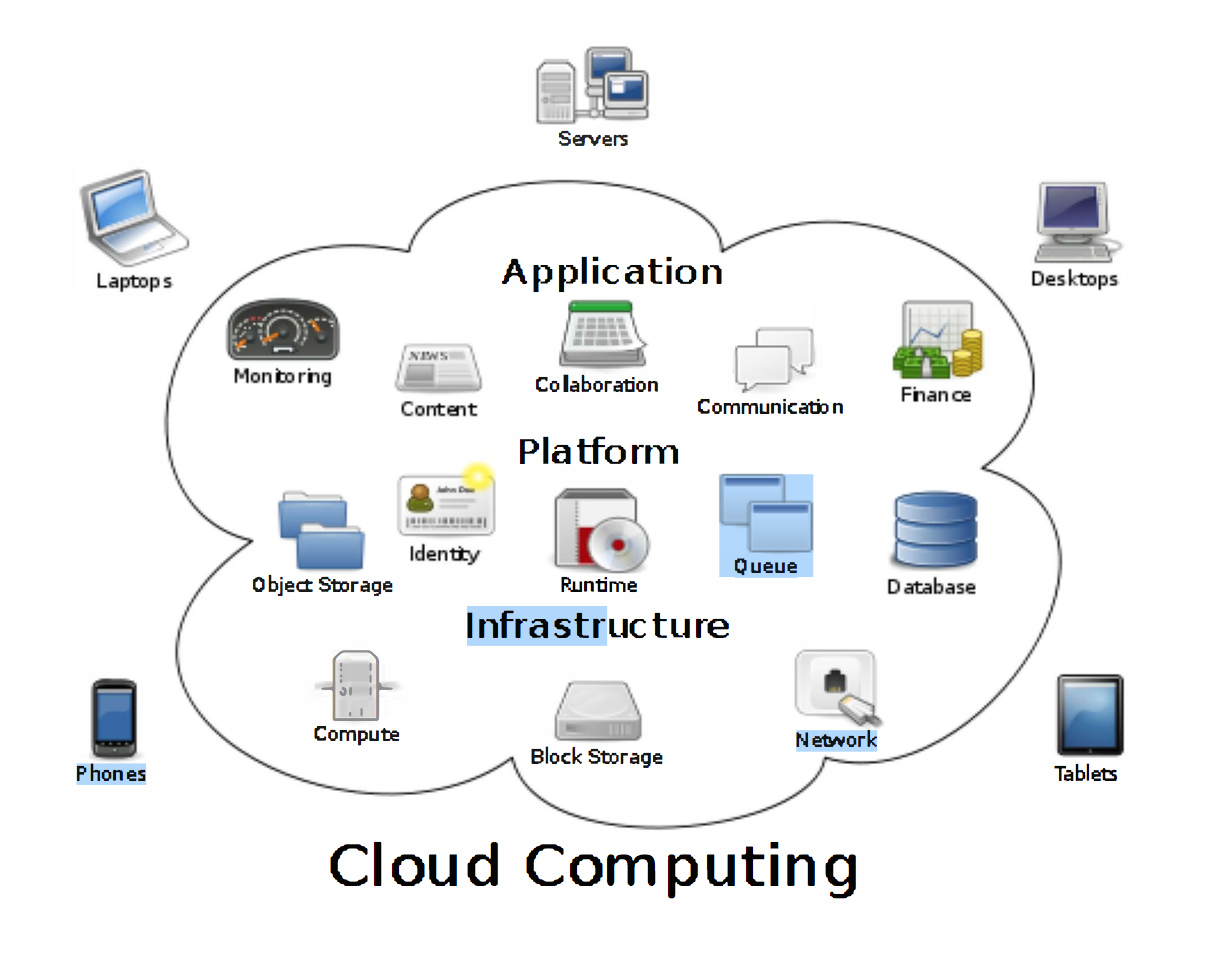
\includegraphics[width=0.7\textwidth]{cloud.png}
	    \caption{ Cloud Computing.  }
	    \label{fig:cloud}
	\end{figure}

		Το μοντέλο cloud αποτελείται από πέντε βασικά χαρακτηριστικά:
		\begin{itemize}
		\item Αυτοεξυπηρέτηση μετά από ζήτηση (On-demand self-service). Ο χρήστης των υπηρεσιών του νέφους μπορεί να χρησιμοποιεί τους υπολογιστικούς πόρους που χρειάζεται, όπως χρόνο στον server και αποθηκευτικό χώρο, αυτόματα και χωρίς να απαιτείται ανθρώπινη αλληλεπίδραση με τον φορέα παροχής υπηρεσιών. 
		\item Ευρεία πρόσβαση στο δίκτυο (Broad network access). Οι δυνατότητες που προσφέρονται είναι διαθέσιμες μέσω του δικτύου και προσβάσιμες μέσω τυποποιημένων μηχανισμών που προωθούν την χρήση ετερογενών πλατφορμών λεπτών ή παχέων πελατών (π.χ., κινητά τηλέφωνα, τάμπλετ, υπολογιστές). 
		\item Διάθεση των πόρων. Οι υπολογιστικοί πόροι των cloud παρόχων είναι συγκεντρωμένοι με χρήση ενός μοντέλου πολλαπλών ενοικιαστών (κάθε οργανισμός εργάζεται με ένα προσαρμοσμένο εικονικό στιγμιότυπο της εφαρμογής), έτσι ώστε να  μπορούν να ανατεθούν οι φυσικοί και εικονικοί πόροι ανάλογα με την ζήτηση των καταναλωτών. Οι παρεχόμενοι πόροι μπορεί να περιλαμβάνουν πόρους όπως μνήμη, επεξεργαστική ισχύ, εύρος δικτύου, εικονικές μηχανές.
		\item Μεγάλη ελαστικότητα (Rapid Elasticity). Οι δυνατότητες του cloud computing παρέχονται με μεγάλη ταχύτητα και προσαρμοστικότητα , ώστε να είναι σε θέση να κλιμακώνουν πολύ γρήγορα ανάλογα με την ζήτηση που υπάρχει και να φαίνονται απεριόριστες σε οποιαδήποτε ποσότητα και χρονική στιγμή ζητηθούν. 
		\item Μετρούμενη υπηρεσία (Measured Service). Τα cloud computing συστήματα πραγματοποιούν μετρήσεις, σε συγκεκριμένα επίπεδα αφαίρεσης ανάλογα με το είδος της υπηρεσίας (επεξεργασία, μνήμη, ενεργοί λογαριασμοί χρηστών). Με βάση αυτές τις μετρήσεις γίνεται έλεγχος και ενέργειες για τη βελτιστοποίηση της χρήσης των πόρων. Επιπλέον η χρήση των πόρων παρακολουθείται, ελέγχεται και καταγράφεται με αποτέλεσμα την παροχή διαφάνειας μεταξύ του χρήστη και του παρόχου του cloud.
		\end{itemize}	\cite{characteristicsCloud}\cite{nist}.

Το cloud computing μπορεί να διαχωριστεί με βάση τις υπηρεσίες που προσφέρει σε διάφορες κατηγορίες. Οι πιο βασικές, είναι α) η υποδομή ως μία υπηρεσία (IaaS), β) η πλατφόρμα ως μία υπηρεσία (PaaS) γ) το λογισμικό ως μία υπηρεσία (SaaS) και το δ) backend των κινητών σαν υπηρεσία(MBaaS), που είναι γνωστό σαν backend σαν υπηρεσία(BaaS).
\\*
		\subsubsection{IaaS}

		Η υποδομή σαν υπηρεσία προσφέρει πρόσβαση σε υπολογιστικούς πόρους στο εικονικό περιβάλλον του cloud, σε εικονικό υλικό (hardware). Το εικονικό υλικό περιλαμβάνει εικονικό χώρο server, συνδέσεις δικτύου, εύρος ζώνης, διευθύνσεις IP  και εξισορροπιστές φορτίου. Το σύνολο των πόρων του υλικού προκύπτει από ένα πλήθος servers και δικτύων που είναι κατανεμημένοι συνήθως σε διάφορα κέντρα δεδομένων και ο πάροχος cloud είναι υπεύθυνος για τη διατήρηση τους. Στον χρήστη δίνεται πρόσβαση στους πόρους του cloud ώστε να μπορεί να χτίσει τις δικές του πλατφόρμες πληροφορικής. 
		
		Οι IaaS υπηρεσίες μπορούν σε συνδυασμό με άλλες υπηρεσίες του cloud να χρησιμοποιηθούν για τη δημιουργία οικονομικά συμφέρουσων και εύκολα επεκτάσιμων λύσεων πληροφορικής, όπου οι δυσκολίες και τα έξοδα διαχείρισης έχουν ανατεθεί στον πάροχο cloud. Όταν οι δραστηριότητες του χρήστη κλιμακώνονται, και επιθυμεί μία επέκταση ή σμίκρυνση των υπολογιστικών πόρων, τότε μπορεί να αντλήσει ή να εγκαταλείψει πόρους cloud χωρίς να χρειάζεται να αγοραστεί, να εγκατασταθεί και να ενσωματωθεί νέο υλικό από τον ίδιο. \cite{IaasService}
		
		Η υπηρεσία IaaS προσφέρει επεκτασιμότητα. Οι πόροι είναι διαθέσιμοι την χρονική στιγμή που τους χρειάζεται ο πελάτης και έτσι αποφεύγονται καθυστερήσεις στην επέκταση της παραγωγικής ικανότητας. Επιπλέον, δεν υπάρχει η ανάγκη για επενδύσεις στο υλικό (hardware). Το "φυσικό" υλικό, το οποίο βρίσκεται πίσω από την IaaS υπηρεσία, έχει στηθεί και συντηρείται από τον πάροχο cloud, με αποτέλεσμα να εξοικονομείται χρόνος και χρήμα στην πλευρά του χρήστη.  Ένα βασικό πλεονέκτημα είναι ότι ο πελάτης κοστολογείται με βάση τη χρήση και πληρώνει μόνο τους πόρους που χρησιμοποιεί. Οι υπηρεσίες μπορούν να προσεγγισθούν από οποιαδήποτε τοποθεσία, αρκεί ο χρήστης να έχει πρόσβαση στο ίντερνετ και τα κατάλληλα διαπιστευτήρια, γεγονός που εξασφαλίζει ανεξαρτησία σε σχέση με την τοποθεσία. Τέλος, στις υπηρεσίες IaaS δεν υπάρχει περίπτωση κατάρρευσης ή βλάβης στο σύστημα, καθώς ακόμα και αν ένας server ή ένας διακόπτης δικτύου πέσει, η ευρύτερη υπηρεσία θα παραμείνει ανεπηρέαστη λόγω των υπόλοιπων πόρων υλικού καθώς και των επιπλέον ρυθμίσεων. Στις περισσότερες περιπτώσεις, ακόμα και αν έπεφτε ολόκληρο το κέντρο δεδομένων, και συνέχιζε να λειτουργεί μόνο ένας server, αυτό θα ήταν αρκετό ώστε οι IaaS υπηρεσίες να εξακολουθούν να τρέχουν ανεμπόδιστα. Ένα μειονέκτημα που υπάρχει είναι ότι σε περιπτώσεις που υπάρχει ανάγκη αλληλεπίδρασης υψηλής ταχύτητας μεταξύ του εσωτερικού λογισμικού ή του λογισμικού που υπάρχει σε κάποιο άλλο cloud και του παρόχου υπηρεσιών IaaS Cloud, μέσω μίας Internet σύνδεσης, μπορεί να μην γίνεται να επιτευχθεί η ταχύτητα που χρειάζεται. \cite{images}
	\\*	
		
		\begin{figure}[h]
	    \centering
	    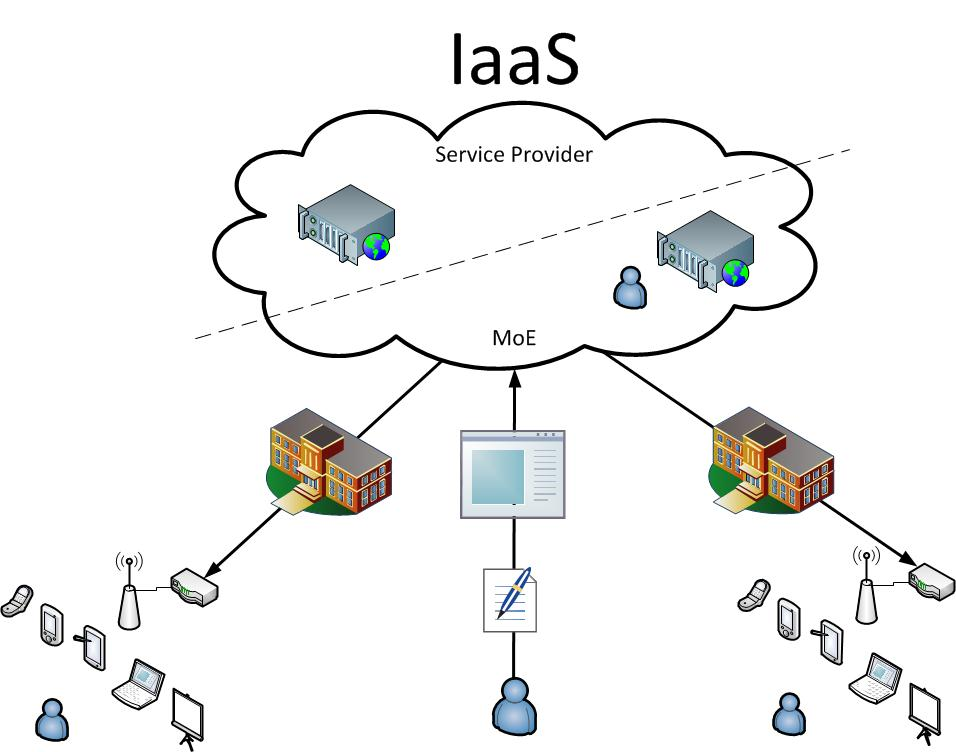
\includegraphics[width=0.7\textwidth]{IaaS.jpg}
	    \caption{ Υπηρεσίες IaaS cloud computing.}
	    \label{fig:iaas}
	\end{figure}
		
		\subsubsection{PaaS}
	
		Η πλατφόρμα σαν υπηρεσία παρέχει στους πελάτες του υπολογιστικού νέφους όλους τους πόρους και τα εργαλεία που απαιτούνται για να έχουν την δυνατότητα να αναπτύξουν, να διαχειριστούν και να τρέξουν εφαρμογές στο διαδίκτυο χωρίς την πολυπλοκότητα και την ανάγκη εγκατάστασης της υποδομής (λογισμικού) που συνήθως συνδέονται με την ανάπτυξη και την έναρξη μιας εφαρμογής. Οι πλατφόρμες σαν υπηρεσίες προσφέρονται σε δύο διαφορετικές μορφές: είτε σαν δημόσιες cloud υπηρεσίες από τον πάροχο, στις οποίες ο χρήστης ελέγχει την ανάπτυξη του λογισμικού και τις ρυθμίσεις διαμόρφωσης, ενώ ο πάροχος εξασφαλίζει το απαραίτητο υπόβαθρο που χρειάζεται η εφαρμογή, είτε σαν λογισμικό, που εγκαθίσταται σε ιδιωτικά κέντρα δεδομένων ή δημόσια υποδομή ως υπηρεσία και διοικείται από εσωτερικά συστήματα πληροφορικής. \cite{Peng2009}
		
		Στο μοντέλο PaaS ο χρήστης δεν ελέγχει την υποκείμενη cloud υποδομή, η οποία συμπεριλαμβάνει το δίκτυο, τους servers, το λειτουργικό σύστημα και τους αποθηκευτικούς χώρους αλλά έχει τον πλήρη έλεγχο στις εγκατεστημένες ή αναπτυγμένες εφαρμογές καθώς και στις ρυθμίσεις των παραμέτρων που γίνονται στο περιβάλλον. Το μοντέλο PaaS βασίζεται σε χρήση της HTML ή Javascript. Υπάρχουν διάφοροι τύποι του μοντέλου PaaS, δημόσιοι, ιδιωτικοί και υβριδικοί. Σε αυτού του τύπου το μοντέλο παροχής υπηρεσιών cloud απαιτούνται δύο επίπεδα προστασίας για τη διασφάλιση της ασφάλειας της ιδιωτικής ζωής. Στο χαμηλότερο επίπεδο του συστήματος, ο πάροχος cloud μπορεί να παρέχει βασικούς μηχανισμούς ασφαλείας, όπως end-to-end κρυπτογράφηση, έλεγχο ταυτότητας και εξουσιοδότηση. Στο υψηλότερο επίπεδο, ο  χρήστης των υπηρεσιών cloud χρειάζεται να καθορίσει τις πολιτικές ελέγχου της πρόσβασης στην εφαρμογή.\cite{Kanagaraj2011}
		
		Στα κύρια πλεονεκτήματα του μοντέλου PaaS συγκαταλέγεται αρχικά το γεγονός ότι επιτρέπει τον προγραμματισμό υψηλού επιπέδου. Επιπροσθέτως, καθιστά την ολική ανάπτυξη μίας εφαρμογής πιο αποτελεσματική, εφόσον έχει ενσωματωμένη δομή, και τη συντήρηση-βελτίωση της πιο εύκολη. Ένα άλλο σημαντικό πλεονέκτημα αποτελεί η υψηλή διαθεσιμότητα, η ελαστικότητα και η ευελιξία που προσφέρει σε συνδυασμό με τις ικανότητες πλήρους αυτοδιαχείρισης και αυτό-κλιμάκωσης της υποδομής και της πλατφόρμας εφαρμογών. Βασικό μειονέκτημα αποτελεί η έλλειψη δια-λειτουργικότητας και η ανικανότητα μεταφοράς της εφαρμογής από έναν πάροχο σε κάποιον άλλον. 

	\begin{figure}[h]
	    \centering
	    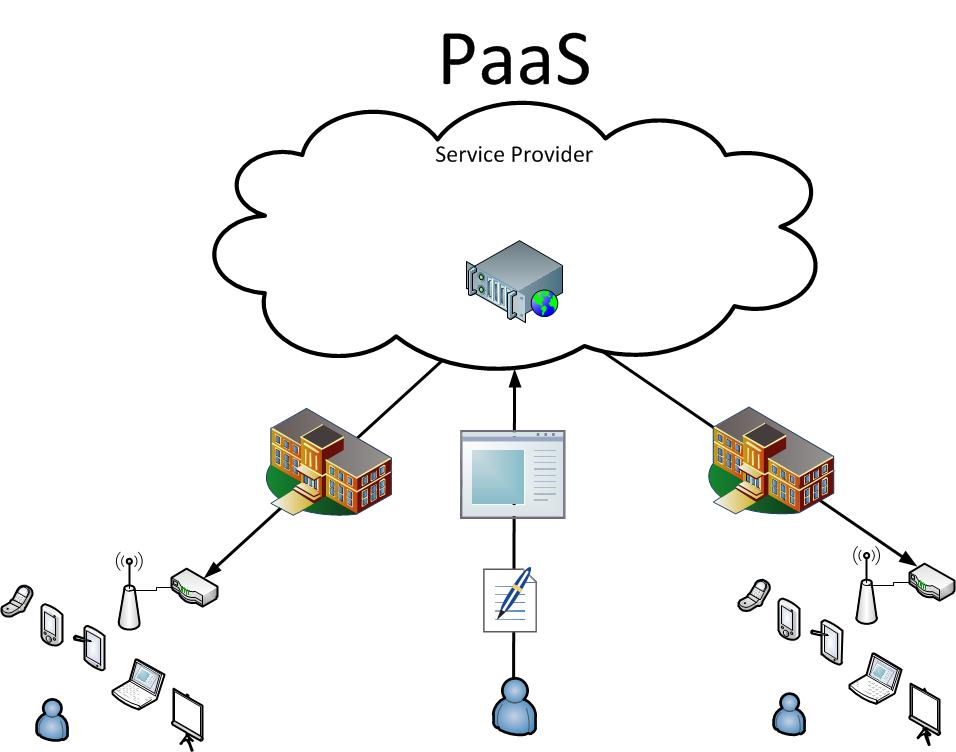
\includegraphics[width=0.7\textwidth]{PaaS.jpg}
	    \caption{Υπηρεσίες PaaS cloud computing.}
	    \label{fig:paas}
	\end{figure}

		\subsubsection{SaaS}
	 
	Το λογισμικό σαν υπηρεσία είναι ένα μοντέλο ανάπτυξης λογισμικού σύμφωνα με το οποίο παρέχονται κατόπιν ζήτησης στον χρήστη εφαρμογές και υπολογιστικοί πόροι. Ουσιαστικά, είναι όλες οι υπηρεσίες του cloud, μέσω των οποίων, οι χρήστες είναι σε θέση να αποκτήσουν πρόσβαση σε εφαρμογές μέσω σύνδεσης στο Internet. Οι εφαρμογές αυτές βρίσκονται στο cloud και μπορούν να χρησιμοποιηθούν για ένα ευρύ φάσμα δραστηριοτήτων, τόσο από εταιρείες όσο και από άτομα. Η χρήση των εφαρμογών αυτών αποτελεί περισσότερο ενοικίαση λογισμικού παρά αγορά του. Με την παραδοσιακές διαδικασία για τις εφαρμογές λογισμικού αρχικά αγοράζεται το λογισμικό ως πακέτο και εγκαθίσταται σε έναν υπολογιστή, ενώ συνήθως οι σχετικές άδειες περιορίζουν τον αριθμό των χρηστών και των συσκευών όπου μπορεί να αναπτυχθεί το λογισμικό. Εν αντιθέσει, οι χρήστες των υπηρεσιών SaaS εγγράφονται στο λογισμικό, χωρίς να το αγοράσουν και επομένως γλιτώνοντας όλη αυτήν τη διαδικασία, και ανανεώνουν τη συνδρομή τους συνήθως σε μηνιαία βάση. 
	
	Οι περισσότεροι χρήστες χρησιμοποιούν έναν λεπτό πελάτη (thin client) για να αποκτήσουν πρόσβαση στις υπηρεσίες SaaS. Οι εταιρικοί χρήστες χρησιμοποιούν τις εφαρμογές που παρέχει ο πάροχος cloud για ανάγκες όπως λογισμικό γραφείου, λογισμικό ανταλλαγής μηνυμάτων,  λογισμικό λογιστικής και τιμολόγησης, λογισμικό παρακολούθησης επιδόσεων, λογισμικό διαχείρισης επιχειρησιακών σχέσεων και άλλα. 
	
	Βασικά πλεονεκτήματα των υπηρεσιών SaaS είναι η ευελιξία και η επεκτασιμότητα που προσφέρουν, καθώς οι χρήστες δεν χρειάζεται να αγοράσουν άλλο λογισμικό ή άλλον server, απλά ενεργοποιούν νέες προσφορές του μοντέλου SaaS. Πολύ σημαντικό είναι επίσης, η υψηλή ποιότητα των υπηρεσιών η υψηλή σταθερότητα και το γεγονός ότι απαιτείται ελάχιστη συντήρηση. Υπάρχει μεγάλο χρονικό κέρδος, καθώς στις υπηρεσίες SaaS το λογισμικό είναι ήδη εγκατεστημένο και ρυθμισμένο και η εφαρμογή μπορεί να διατεθεί στον χρήστη έτοιμη για χρήση. Η πολιτική κοστολόγησης της χρήσης των υπηρεσιών είναι ιδιαίτερα συμφέρουσα συγκριτικά με την αγορά του και πολλές φορές επιτρέπει την χρήση εφαρμογών που σε άλλη περίπτωση θα ήταν απαγορευμένες, λόγω ιδιαίτερα υψηλού κόστους. Θεωρείται αξιόπιστη λύση ασφαλείας, καθώς υιοθετεί SSL (Secure Socket Layer) στις υπηρεσίες του με αποτέλεσμα τα δεδομένα να μεταδίδονται από και προς τον χρήστη με ασφάλεια. Βασικό μειονέκτημα αποτελεί το γεγονός ότι παρέχει πρόσβαση βασισμένη σε ένα δίκτυο που αποτελείται από τις περισσότερο εμπορικές εφαρμογές με αποτέλεσμα να μην μπορεί πάντα κάποιος να βρει το λογισμικό που ψάχνει διαθέσιμο στο SaaS. 
	
		\begin{figure}[h]
	    \centering
	    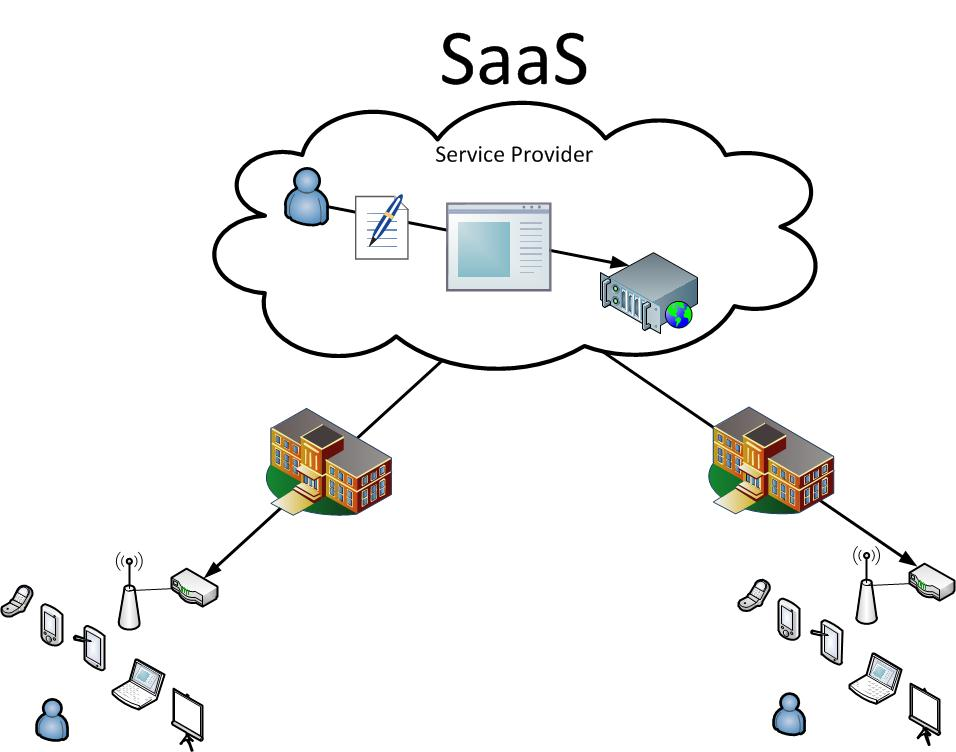
\includegraphics[width=0.7\textwidth]{SaaS.jpg}
	    \caption{Υπηρεσίες SaaS cloud computing.}
	    \label{fig:saas}
	\end{figure}
	
		\subsubsection{BaaS}
 
	
	Η υπηρεσία BaaS είναι ένα μοντέλο που παρέχει στους προγραμματιστές διαδικτυακών εφαρμογών και εφαρμογών για κινητά τηλέφωνα έναν τρόπο εύκολης και γρήγορης διασύνδεσης των εφαρμογών, μέσω παρεχόμενων APIs. Παρέχει υπηρεσίες όπως διαχείριση χρηστών, ειδοποιήσεις (push notifications), κώδικα για server και σύνδεση με υπηρεσίες κοινωνικών δικτύων.  Όλες αυτές οι υπηρεσίες αξιοποιούνται μέσω χρήσης εργαλείων ανάπτυξης λογισμικού (SDKs) και έχουν την δική τους διεπαφή προγραμματισμού εφαρμογών (APIs), που τους επιτρέπει να ενσωματωθούν στις εφαρμογές χωρίς ιδιαίτερο κόπο. Η παροχή ενός σταθερού τρόπου για την διαχείριση των backend δεδομένων συνεπάγεται το γεγονός ότι οι προγραμματιστές δεν χρειάζεται να αναπτύξουν κώδικα backend για κάθε υπηρεσία που χρησιμοποιεί ή έχει πρόσβαση η εφαρμογή τους.

	Ένα από τα κύρια πλεονεκτήματα της χρήσης υπηρεσιών BaaS είναι η τεράστια μείωση του χρόνου ολοκλήρωσης και συντήρησής της εφαρμογής , σε ποσοστό μέχρι και 60\%. Επιπλέον ευνοείται η κλιμάκωση, καθώς το BaaS παρέχει ένα συγκεκριμένο backend το οποίο διαμορφώνει κάποιος εύκολα με βάση τις ανάγκες της εφαρμογής. Η ανάλυση της εφαρμογής γίνεται πιο αποδοτική, καθώς το BaaS διαχειρίζεται όλη τη "κίνηση" που γίνεται μέσα στην εφαρμογή και αναλύει τι συμβαίνει σε αυτήν (ποιοι χρήστες είναι πιο ενεργοί, ποιοι είναι πιο εμπλεκόμενοι κ.λ.π. ). Παρά τα πολλά οφέλη του BaaS, είναι επίσης σημαντικό να ληφθεί υπόψιν η κατασκευή του user-interface (UI), διότι αυτό βρίσκεται σε άμεση επικοινωνία με τους τελικούς χρήστες. Ο ρόλος του UI είναι να συνδέεται η εφαρμογή με άλλα ανεξάρτητα κομμάτια ή με αποκλειστικά APIs που συνδέονται στο backend, κάτι το οποίο με χρήση των υπηρεσιών BaaS δεν είναι δυνατό πολλές φορές καθώς μια εφαρμογή "κλειδώνεται" στον πάροχο.
	
		\begin{figure}[h]
	    \centering
	    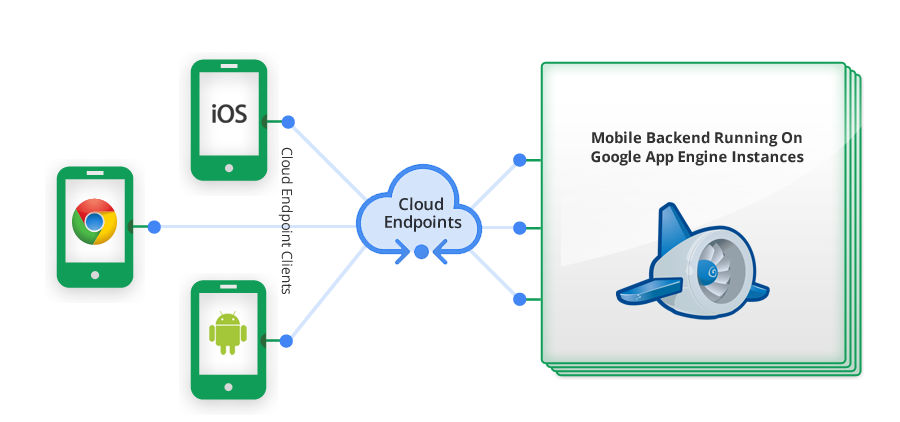
\includegraphics[width=0.7\textwidth]{BaaS.png}
	    \caption{Υπηρεσίες BaaS cloud computing. }
	    \label{fig:baas}
	\end{figure}

	Στην συνέχεια θα αναπτυχθούν τα μοντέλα ανάπτυξης του cloud computing.
	\subsubsection{Public cloud}
	
 
		Το δημόσιο cloud computing είναι ένα μοντέλο μέσω του οποίου οι χρήστες έχουν πρόσβαση στο cloud μέσω διεπαφών που χρησιμοποιούν τα προγράμματα περιήγησης. Ένα cloud καλείται δημόσιο, όταν οι υπηρεσίες του παρέχονται μέσω ενός δημόσιου δικτύου, όπως το Internet και είναι ανοιχτές για δημόσια χρήση. Τα δημόσια cloud παρέχουν υπηρεσίες σε πολλούς πελάτες χρησιμοποιώντας την ίδια διαμοιραζόμενη υποδομή.Πολλά δημόσια cloud δεν χρεώνουν τον χρήστη.
		
		 Οι υπηρεσίες SaaS όπως η αποθήκευση στο cloud και οι online εφαρμογές γραφείου είναι οι υπηρεσίες που βρίσκονται κατά κόρον σε δημόσια cloud. Οι υπηρεσίες υποδομής (IaaS) καθώς και οι πλατφόρμες σαν υπηρεσία (PaaS), κυρίως οι περιπτώσεις του cloud web hosting και των περιβαλλόντων ανάπτυξης, αναπτύσσονται εξίσου συχνά και σε δημόσια και σε ιδιωτικά cloud. Τα δημόσια cloud χρησιμοποιούνται ευρέως σε προσφορές για ιδιώτες οι οποίοι είναι λιγότερο πιθανόν να χρειαστούν το επίπεδο των υποδομών και την ασφάλεια που προσφέρουν τα ιδιωτικά cloud. Ωστόσο, σε πολλές περιπτώσεις οι επιχειρήσεις μπορούν να χρησιμοποιούν δημόσια cloud σε περιπτώσεις που δεν τίθεται θέμα ευαίσθητων δεδομένων (π.χ. webmai, online συνεργασία) για να κάνουν τις λειτουργίες τους πιο αποτελεσματικά \cite{characteristics}.

			Τα βασικά πλεονεκτήματα του δημόσιου cloud είναι:
			\begin{itemize}

			\item Απόλυτη επεκτασιμότητα. Το γεγονός ότι οι υπολογιστικοί πόροι στο cloud είναι "ανεξάντλητοι" και γίνονται διαθέσιμοι ανάλογα με τη ζήτηση έχει ως αποτέλεσμα οι εφαρμογές που τρέχουν σε αυτούς να μπορούν να ανταποκριθούν στις διακυμάνσεις της δραστηριότητας.
			
			\item Υψηλή απόδοση. Τα δημόσια cloud συνεπάγονται υψηλότερα επίπεδα υπολογιστικών πόρων με ταυτόχρονα λιγότερο κόστος. Μερικές προτάσεις μαζικής αγοράς μπορούν ακόμη και να είναι δωρεάν για τον πελάτη και να στηρίζονται στις διαφημίσεις για τα έσοδα τους (Google).
			
			\item Το μοντέλο πληρωμής ανάλογα με τη χρήση. Ο χρήστης είναι σε θέση να αποκτήσει πρόσβαση στους πόρους που χρειάζεται, όποτε θέλει και να πληρώσει μόνο για αυτούς που χρησιμοποιεί αποφεύγοντας τους περιττούς πόρους.

			\item 	Ευελιξία. Υπάρχει ένας τεράστιος αριθμός των IaaS, PaaS και SaaS υπηρεσιών που διατίθενται στην αγορά, οι οποίες ακολουθούν το μοντέλο του δημόσιου cloud και τις οποίες ο χρήστης μπορεί να προσεγγίσει από οποιαδήποτε συσκευή με χρήση Internet. Οι υπηρεσίες αυτές μπορούν να εκπληρώσουν τις περισσότερες υπολογιστικές απαιτήσεις και μπορούν να χρησιμοποιηθούν εξίσου αποτελεσματικά  από ιδιώτες και επιχειρήσεις. 
			
			\item Ανεξαρτησία της τοποθεσίας. Η διαθεσιμότητα των υπηρεσιών του δημόσιου cloud μέσω του Internet, εξασφαλίζει ότι οι υπηρεσίες είναι διαθέσιμες όπου και αν βρίσκεται ο χρήστης. Αυτό το γεγονός πολλές φορές είναι ιδιαίτερα χρήσιμο όπως για παράδειγμα σε περιπτώσεις εταιριών, όπου δίνεται η δυνατότητα για απομακρυσμένη πρόσβαση σε υποδομές πληροφορικής (σε περίπτωση έκτακτης ανάγκης, κ.λ.π.).
			
		\end{itemize}
			
			
	\subsubsection{Private cloud}

	 
	Το ιδιωτικό cloud, είναι ένα μοντέλο το οποίο λειτουργεί αποκλειστικά για έναν οργανισμό, διευθύνεται είτε από τον ίδιο τον οργανισμό είτε από τρίτους και εγκαθίσταται είτε εσωτερικά είτε εξωτερικά. Περιλαμβάνει ένα ξεχωριστό και ασφαλές περιβάλλον με το οποίο μπορούν να αλληλεπιδράσουν οι χρήστες. Τα ιδιωτικά cloud παρέχουν μεγάλη υπολογιστική ισχύ σαν υπηρεσία χρησιμοποιώντας ένα σύνολο από φυσικούς υπολογιστικούς πόρους, οι οποίοι είναι προσβάσιμοι μόνο από έναν οργανισμό, εξασφαλίζοντας περισσότερο έλεγχο και αυξημένη ασφάλεια. Τα δημόσια cloud περιλαμβάνουν πολλούς πελάτες οι οποίοι έχουν πρόσβαση σε εικονικές υπηρεσίες που αντλούν πόρους από την ίδια ομάδα από servers μέσω δημοσίων δικτύων. Τα ιδιωτικά cloud από την άλλη πλευρά, περιλαμβάνουν την οριοθέτηση ενός cloud για την αποκλειστική χρήση από έναν οργανισμού. Παρόλο που χρησιμοποιούνται ξεχωριστοί πόροι, μπορούν να γίνουν προσβάσιμοι μέσω ιδιωτικών γραμμών ή ασφαλών κρυπτογραφημένων συνδέσεων δημόσιου δικτύου \cite{Doelitzscher2011} \cite{Missbach}.
	
	Τα ιδιωτικά cloud είναι κατάλληλα για περιπτώσεις στις οποίες υπάρχει η ανάγκη αποθήκευσης και επεξεργασίας ιδιωτικών ή ευαίσθητων δεδομένων ή η ανάγκη διεξαγωγής ευαίσθητων εργασιών. Για παράδειγμα, μία ιδιωτική cloud υπηρεσία μπορεί να χρησιμοποιηθεί από ένα πληροφοριακό σύστημα που διαχειρίζεται και αποθηκεύει ευαίσθητα ιατρικά δεδομένα και θέλει να επωφεληθεί από τα πλεονεκτήματα του cloud computing στην επιχειρησιακή υποδομή του. 	Υιοθετεί τις βασικές αρχές ασφαλείας, νομοθεσίας και κανονιστικών απαιτήσεων αφού προσφέρει μεγάλο έλεγχο εγκατάστασης και χρήσης στην επιχείρηση που το χρησιμοποιεί. Το ιδιωτικό μοντέλο cloud μοιάζει αρκετά με το μοντέλο των δικτύων τοπικής πρόσβασης (LAN) που χρησιμοποιούταν στο παρελθόν αλλά παρέχει τα επιπλέον πλεονεκτήματα του cloud. Κάποια από τα πλεονεκτήματα του ιδιωτικού cloud είναι:
	
	\begin{itemize}
	
	\item Μεγαλύτερη προστασία και ασφάλεια. Τα δημόσια cloud εφαρμόζουν μηχανισμούς παροχής ασφάλειας, αλλά τα ιδιωτικά cloud με τους αποκλειστικούς φυσικούς πόρους, οι οποίοι επιτρέπουν πρόσβαση μόνο σε συνδέσεις που γίνονται μέσω συγκεκριμένου οργανισμού και προσωπικές ασφαλείς γραμμές εξασφαλίζουν ότι υπάρχει πλήρης ασφάλεια και αξιοπιστία.
	
	\item Περισσότερο έλεγχο με αποτέλεσμα περισσότερη ευελιξία. Εφόσον η πρόσβαση στους πόρους γίνεται μόνο από έναν οργανισμό, αυτός ο οργανισμός έχει την ικανότητα να ρυθμίσει και να διαχειριστεί το cloud όπως επιθυμεί, ώστε να επιτευχθεί το κατάλληλο δίκτυο. 
	
	\item Βελτίωση  της σχέσης κόστους και ενεργειακής απόδοσης. Η εφαρμογή ενός ιδιωτικού μοντέλου cloud μπορεί να συντελέσει στην καλύτερη κατανομή των πόρων σε έναν οργανισμό, εξασφαλίζοντας ότι η διαθεσιμότητα των πόρων ανταποκρίνεται άμεσα και ευέλικτα ανάλογα με τη ζήτηση τους. Παρόλο που είναι πιο ακριβά σε σχέση με τα δημόσια cloud, κάνουν πιο αποτελεσματική χρήση των υπολογιστικών πόρων σε σχέση με τα παραδοσιακά τοπικά δίκτυα (LANs), καθώς ελαχιστοποιείται η επένδυση σε αχρησιμοποίητη παραγωγική ικανότητα. 
	
	\item Βελτιωμένη αξιοπιστία. Ακόμα και αν οι πόροι (servers, δίκτυα, κ.λ.π.) φιλοξενούνται εσωτερικά στον πελάτη, η δημιουργία εικονικών περιβάλλοντων λειτουργικού συνεπάγεται ότι το δίκτυο είναι πιο ανθεκτικό σε επιμέρους αστοχίες από ότι η φυσική υποδομή. 

	\end{itemize}
	
		
		\subsubsection{Community cloud}
		
		Το κοινοτικό cloud είναι ένα μοντέλο νέφους το οποίο μοιράζεται σε διάφορους οργανισμούς και υποστηρίζει μια συγκεκριμένη κοινότητα που έχει κοινά ενδιαφέροντα (ασφάλειας,  συμμόρφωσης, της διεθνούς δικαιοδοσίας, κλπ). Η διαχείριση του νέφους μπορεί να γίνει είτε εσωτερικά  από τον ίδιο τον οργανισμό είτε από τρίτους και υλοποιείται είτε εντός είτε εκτός του οργανισμού. Οι δαπάνες κατανέμονται σε λιγότερους χρήστες από ότι σε ένα δημόσιο cloud (περισσότερους βέβαια από ότι σε ένα ιδιωτικό cloud), και έτσι πραγματοποιούνται μόνο μερικές από τις δυνατότητες εξοικονόμησης κόστους του cloud computing \cite{Briscoe2009} \cite{condori}.
	
	Το κοινοτικό cloud φιλοδοξεί να συνδυάσει την υπολογιστική παροχή των πόρων που διανέμονται από το δίκτυο, τον κατανεμημένο έλεγχο από τα ψηφιακά οικοσυστήματα και τη βιωσιμότητας της "πράσινης" πληροφορικής, με τις περιπτώσεις χρήσης του cloud computing, κάνοντας μεγαλύτερη χρήση των πλεονεκτημάτων της αυτοδιαχείρισης του υπολογιστικού συστήματος. Τα πλεονεκτήματα του κοινοτικού cloud περιλαμβάνουν:
	\begin{itemize}
	
	\item Χαμηλότερο κόστος. Το κόστος της δημιουργίας ενός κοινοτικού cloud έναντι των ιδιωτικών cloud μπορεί να είναι χαμηλότερο λόγω της κατανομή των κοστών σε όλους τους συμμετέχοντες.

	\item Ανάθεση της διαχείρισης σε έναν πάροχο cloud. Το πλεονέκτημα έγκειται στο γεγονός ότι ο πάροχος θα είναι ένας αμερόληπτος τρίτος που δεσμεύεται από σύμβαση και δεν έχει καμία προτίμηση σε κάποιον από τους πελάτες που εμπλέκονται.
	
	\end{itemize}

Βασικό μειονέκτημα αποτελεί το γεγονός ότι το κόστος είναι πολύ υψηλότερο από ότι στα δημόσια cloud \cite{cloudOverview}.

		
		
		
		\subsubsection{Hybrid cloud}
		
		Τα υβριδικά cloud είναι μία ολοκληρωμένη υπηρεσία που αποτελείται από δύο ή περισσότερα cloud (ιδιωτικά, δημόσια ή κοινοτικά) τα οποία παραμένουν ξεχωριστές οντότητες αλλά συνδέονται μεταξύ τους, προσφέροντας τα πλεονεκτήματα των πολλαπλών μοντέλων ανάπτυξης. Μια υπηρεσία υβριδικού cloud ξεπερνά τα όρια του παρόχου σε σχέση με τις άλλες υπηρεσίες cloud,  με αποτέλεσμα να μην μπορεί να κατηγοριοποιηθεί απλά σε μία κατηγορία ιδιωτικών, δημόσιων ή κοινοτικών υπηρεσιών cloud. Με τα υβριδικά cloud μπορεί να επεκταθεί η ικανότητα ή η χωρητικότητα μιας υπηρεσίας μέσω της ένταξης ή της προσαρμογής της με κάποια άλλη υπηρεσία cloud \cite{palwe}.
		
		Η επιλογή υλοποίησης ενός υβριδικού cloud εξαρτάται από έναν αριθμό παραγόντων, όπως οι απαιτήσεις ασφάλειας των δεδομένων και των λειτουργιών πάνω σε αυτά, το επίπεδο ελέγχου που απαιτείται, καθώς και τις εφαρμογές που χρησιμοποιεί ο χρήστης. Όλες οι υπηρεσίες του cloud computing προσφέρουν βελτίωση της αποτελεσματικότητας, αλλά οι υπηρεσίες των δημόσιων cloud υπερτερούν σε σχέση με αυτές των ιδιωτικών λόγω χαμηλότερου κόστους και καλύτερης κλιμάκωσης. Ως εκ τούτου, ένας οργανισμός μπορεί να μεγιστοποιήσει την αποτελεσματικότητα του χρησιμοποιώντας υπηρεσίες από δημόσια cloud για όλες τις μη-ευαίσθητες λειτουργίες, στηριζόμενος σε χρήση ιδιωτικού cloud μόνο όταν κρίνεται τελείως απαραίτητο, και διασφαλίζοντας ότι όλες οι πλατφόρμες συνεργάζονται άψογα μεταξύ τους \cite{Zhou2013}.
		
		Το εξειδικευμένο μοντέλο του υβριδικού cloud, το οποίο είναι χτισμένο πάνω σε ετερογενές hardware, ονομάζεται "Cross-platform Hybrid Cloud". Συνήθως χρησιμοποιούνται διαφορετικές αρχιτεκτονικές επεξεργαστών, για παράδειγμα, x86-64 και ARM. Οι χρήστες μπορούν να αναπτύξουν εφαρμογές με πλήρη διαφάνεια, χωρίς να γνωρίζουν την πολυμορφία του υλικού του cloud. Αυτό το είδος cloud έχει προκύπτει από την αύξηση των βασισμένων σε ARM system-on-chip αρχιτεκτονικών για servers.
		
		Ένα ειδικά διαμορφωμένο υβριδικό cloud, προσφέρει τα εξής πλεονεκτήματα:
		
		\begin{itemize}

		\item Επεκτασιμότητα. Ενώ τα ιδιωτικά cloud προσφέρουν δυνατότητα κλιμάκωσης η οποία εξαρτάται από τις ρυθμίσεις τους (όπως το αν φιλοξενούνται εσωτερικά ή εξωτερικά), οι υπηρεσίες των δημοσίων cloud computing προσφέρουν πολύ αυξημένες δυνατότητες επεκτασιμότητας, διότι οι πόροι τους προέρχονται από μεγαλύτερες υποδομές. Υλοποιώντας τις μη-ευαίσθητες λειτουργίες σε δημόσιο cloud μπορεί ένας οργανισμός να επωφεληθεί από την επεκτασιμότητα του δημόσιου cloud και ταυτόχρονα να μειώσει τις απαιτήσεις στο ιδιωτικό cloud.
		
		\item Εξοικονόμηση κόστους. Τα δημόσια cloud  προσφέρουν με χρήση υπηρεσιών (όπως η κεντρική διαχείριση) μεγαλύτερη αποδοτικότητα κόστους, από τα ιδιωτικά cloud. Ως εκ τούτου, τα υβριδικά σύννεφα επιτρέπουν στους οργανισμούς να έχουν πρόσβαση σε αυτές τις συμφέρουσες υπηρεσίες για όσες από τις λειτουργίες τους είναι εφικτό, διατηρώντας ωστόσο τις ευαίσθητες λειτουργίες ασφαλείς στο ιδιωτικό cloud.

		\item Ασφάλεια. Το ιδιωτικό cloud του μοντέλου υβριδικού cloud παρέχει την απαραίτητη ασφάλεια για τις ευαίσθητες λειτουργίες και επιπλέον σε πολλές περιπτώσεις τηρεί τις προϋποθέσεις για τον χειρισμό και την αποθήκευση δεδομένων.

		\item Ευελιξία. Η διαθεσιμότητα τόσο των ασφαλών πόρων του ιδιωτικού cloud και όσο και των οικονομικότερων των δημοσίων cloud, παρέχει στους οργανισμούς περισσότερες ευκαιρίες για να εξερευνήσουν διαφορετικές επιχειρησιακές κατευθύνσεις.
		\end{itemize} 

		\subsection{NodeJs}
	
		Το Node.js, ή απλούστερα Node, είναι μια πλατφόρμα που μας επιτρέπει να γράψουμε JavaScript στην πλευρά του εξυπηρετητή (server-side JavaScript). Από το 2009, που δημιουργήθηκε, μέχρι σήμερα η πλατφόρμα έχει εξελιχθεί ραγδαία και χρησιμοποιείται σε πολλές μεγάλες εφαρμογές. Αποτελεί αυτήν την στιγμή το δεύτερο σε επισκεψιμότητα πρότζεκτ στο GitHub και έχει παραπάνω από 90000 πακέτα (modules) που έχουν δημοσιευτεί στον διαχειριστή πακέτων του Node (Node Package Manager, NPM). Οι NodeJs εφαρμογές είναι γραμμένες σε JavaScript και μπορούν να εκτελεστούν σε OS X, Microsoft Windows, Linux, FreeBSD, NonStop, IBM AIX, IBM System z και IBM i. Το πρότζεκτ του Node φιλοξενείται και υποστηρίζεται από το Node.js Foundation, ένα συλλογικό έργο του Linux Foundation \cite{Tilkov2010}.

		Το Node είναι μια οδηγούμενη από γεγονότα (event-driven) πλατφόρμα,  στην οποία μια διεργασία σε αντίθεση με τα περισσότερα σύγχρονα περιβάλλοντα ανάπτυξης εφαρμογών  δεν στηρίζεται στην πολυνηματικότητα αλλά χρησιμοποιεί λειτουργίες εισόδου/εξόδου χωρίς αναμονή (non blocking I/O), ή ισοδύναμα χρησιμοποιεί ασύγχρονη Ε/Ε (asynchronous I/O) . Αυτό έχει ως σκοπό να αυξήσει την απόδοση και τη δυνατότητα κλιμάκωσης (scalability) των διαδικτυακών εφαρμογών πραγματικού χρόνου. Το Node χρησιμοποιεί την V8, μια εικονική μηχανή που αναπτύχθηκε από τη Google για τον Google Chrome και τρέχει κώδικα JavaScript. Η V8 δίνει στο Node μεγάλη αύξηση στην απόδοση, καθώς κάνει απευθείας μεταγλώττιση σε γλώσσα μηχανής αντί να εκτελεί bytecode ή να χρησιμοποιεί διερμηνευτή (interpreter).

	Το Node επιτρέπει τη δημιουργία web servers και εργαλείων δικτύωσης με χρήση της γλώσσας JavaScript και μια συλλογή από πακέτα (modules), τα οποία χειρίζονται διάφορες λειτουργίες του πυρήνα \cite{node}. Τα πακέτα αυτά χειρίζονται το σύστημα αρχείων Ε/Ε, το σύστημα δικτύωσης (HTTP, TCP, UDP, DNS, ή TLS / SSL), τα δυαδικά δεδομένα (buffers)] και άλλες βασικές λειτουργίες. Τα πακέτα του NodeJs χρησιμοποιούν ένα API το οποίο έχει σχεδιαστεί για να μειώσει την πολυπλοκότητα της ανάπτυξης εφαρμογών για διακομιστή.

	Χρησιμοποιείται κυρίως για την κατασκευή προγραμμάτων δικτύου, όπως διακομιστές δικτύου (web servers), γεγονός που το καθιστά παρόμοιο με την PHP και την Python. Η μεγαλύτερη διαφορά μεταξύ PHP και Node είναι ότι η PHP είναι μια γλώσσα με αναμονή, όπου η εκτέλεση των εντολών προχωρά μόνο όταν έχουν ολοκληρωθεί οι προηγούμενες, ενώ στο Node  οι εντολές εκτελούνται παράλληλα και χρησιμοποιούνται  κλήσεις με επιστροφή (callbacks) για να σηματοδοτηθεί η ολοκλήρωση. Το Node υλοποιεί οδηγούμενο από γεγονότα προγραμματισμό για διαδικτυακές εφαρμογές σε JavaScript. Οι προγραμματιστές μπορούν να δημιουργήσουν εξαιρετικά επεκτάσιμους servers χωρίς τη χρήση νημάτων, χρησιμοποιώντας ένα απλοποιημένο οδηγούμενο από γεγονότα μοντέλο προγραμματισμού που χρησιμοποιεί κλήσεις επιστροφή για να σηματοδοτήσει την ολοκλήρωση ενός στόχου\cite{surenda}.

\subsubsection{Javascript}

		Η JavaScript αναπτύχθηκε αρχικά από τον Brendan Eich του Netscape και ονομαζόταν Μόκα, η οποία αργότερα μετονομάστηκε σε LiveScript, και τελικά σε JavaScript. LiveScript ήταν το επίσημο όνομα για τη γλώσσα, όταν εισήχθη για πρώτη φορά σε beta εκδόσεις του Netscape Navigator 2,0 αλλά μετονομάστηκε σε JavaScript σε μια κοινή ανακοίνωση με την Sun Microsystems όταν προοριζόταν να αναπτυχθεί στη νέα έκδοση του Netscape Navigator 2.0B3.

		H JavaScript, επίσης γνωστή ως ECMAScript, είναι μία πρότυπη αντικειμενοστραφής scripting γλώσσα η οποία είναι δυναμική και έχει πρώτης τάξεως λειτουργίες. Η JavaScript είναι μια εφαρμογή του προτύπου γλώσσας ECMAScript και χρησιμοποιείται κυρίως με τη μορφή client-side, όπου υλοποιείται ως μέρος ενός web browser, ώστε να παρέχεται ενισχυμένη διεπαφή χρηστών και δυναμικές ιστοσελίδες. Αυτό επιτρέπει την πρόσβαση μέσω προγραμματισμού στα υπολογιστικά αντικείμενα μέσα σε ένα περιβάλλον υποδοχής. Η JavaScript χρησιμοποιεί σύνταξη επηρεασμένη από αυτή της C. Πολλά ονόματα και συμβάσεις ονοματολογίας έχουν αντιγραφεί από τη Java, αλλά οι δύο γλώσσες είναι διαφορετικές και έχουν πολύ διαφορετική σημασιολογία. Οι βασικές αρχές σχεδιασμού στο πλαίσιο της JavaScript, λαμβάνονται από Self και Scheme γλώσσες προγραμματισμού. Είναι μια γλώσσα συγγραφής σεναρίων (scripting language) για την προσθήκη διαδραστικότητας (interactivity) σε ιστοσελίδες. 
	
		Με την JavaScript μπορούμε να φτιάξουμε σενάρια που να εκτελούν αυτόματες εργασίες, για παράδειγμα όταν μια σελίδα του Web ανοίγει ή κλείνει. Επίσης μπορούμε να χρησιμοποιήσουμε την Javascript για να εκτελέσει ενέργειες που να ανταποκρίνονται σε ένα συγκεκριμένο γεγονός. Για παράδειγμα, όταν ο χρήστης επιλέγει ένα κουμπί, έναν σύνδεσμο ή όταν επιλέγει να εστιάσει από ένα στοιχείο μιας φόρμας σε ένα άλλο στοιχείο της, εκτελείται κώδικας Javascript. 

		Κάθε φυλλομετρητής υλοποιεί τον δικό του διερμηνευτή για την JavaScript (συνήθως καλείται μηχανή JavaScript), ο οποίος μάλιστα είναι και καθοριστικής σημασίας για την απόδοση του φυλλομετρητή όσον αφορά στη συμβατότητα, σταθερότητα, ταχύτητα και ασφάλεια. Συνήθως ο κώδικας JavaScript διερμηνεύεται, δε μεταγλωττίζεται. Εντούτοις για να βελτιωθεί η απόδοση, υπάρχουν φυλλομετρητές που ακολουθούν μεθόδους just-in-time μεταγλώττισης, όπως ο Google Chrome με μια καινοτόμο μηχανή JavaScript, την V8.
		
		Η σύνταξη JavaScript είναι κοινή μεταξύ των διάφορων φυλλομετρητών, παρόλο που υπάρχουν διαφορές στην ονοματολογία των βασικών μεθόδων. Η σύνταξη θυμίζει php, με τη διαφορά ότι δεν χρησιμοποιείται το χαρακτηριστικό «\$» στα ονόματα των μεταβλητών. Πρόκειται για μια γλώσσα χαλαρών τύπων όπου οι μεταβλητές μπορούν να αλλάξουν τύπο δυναμικά. Αλφαριθμητικά μεταβλητού μεγέθους υποστηρίζονται εγγενώς. Για τη δήλωση μιας μεταβλητής χρησιμοποιείται η λέξη-κλειδί "var" ενώ για τον ορισμό συνάρτησης χρησιμοποιείται η λέξη "function" και δεν απαιτείται να δηλωθεί ο τύπος του αποτελέσματος. Δεν υπάρχουν δείκτες, ενώ υποστηρίζονται τάξεις. 

\subsubsection{Javascript στον Εξυπηρετητή (server-side Javascript)}

 
 Μέχρι πρόσφατα η Javascript χρησιμοποιούνταν μόνο στο front-end των προγραμμάτων περιήγησης και οι προγραμματιστές ήταν υποχρεωμένοι να χρησιμοποιούν άλλες γλώσσες για τον προγραμματισμό στον εξυπηρετητή (server) και στον εξυπηρετούμενο (client). Το γεγονός ότι το Node μας δίνει τη δυνατότητα να χρησιμοποιήσουμε την ίδια γλώσσα και στις δύο άκρες, απλουστεύει σημαντικά την ανάπτυξη των διαδικτυακών εφαρμογών.  Με αυτόν τον τρόπο, το μόνο προαπαιτούμενο για να αναπτύξει κανείς μια διαδικτυακή εφαρμογή είναι η γνώση Javascript. Εκτός από τη μεγάλη διευκόλυνση που προσφέρει, το γεγονός ότι χρησιμοποιούμε Javascript και στις δύο πλευρές συντελεί σημαντικά και στην αύξηση της απόδοσης των διαδικτυακών εφαρμογών. Με χρήση του προγράμματος περιήγησης Google Chrome, η ταχύτητα με την οποία εκτελείται η JavaScript αυξάνεται με τρομερά ταχείς ρυθμούς.

Η JavaScript δεν παρέχει κάποια βιβλιοθήκη για λειτουργίες Ε/Ε με σύγχρονο τρόπο και εξαιτίας αυτού  οι λειτουργίες που παρέχονται στην πλατφόρμα Node είναι χωρίς αναμονή (non blocking). Οι συναρτήσεις στην JavaScript αποτελούν αντικείμενα πρώτης τάξης (first-class functions). Αυτό σημαίνει ότι η γλώσσα υποστηρίζει το πέρασμα μιας συνάρτησης σαν παράμετρο σε μια άλλη συνάρτηση και την επιστροφή μιας συνάρτησης σαν αποτέλεσμα από μια άλλη συνάρτηση. Επιπλέον, η JavaScript παρέχει το μοτίβο κλεισίματος (closure pattern). Με αυτόν τον τρόπο οι συναρτήσεις επιστρεφόμενης κλήσης (callback functions) έχουν την ιδιότητα να κρατάνε στοιχεία και να ξέρουν το περιβάλλον λειτουργίας στο οποίο δηλώθηκαν και τις μεταβλητές που υπήρχαν σε αυτό το περιβάλλον. Το Node στηρίζεται στα παραπάνω δύο χαρακτηριστικά της Javascript.

\subsubsection{Νήματα, μονονηματικό μοντέλο και πολυνηματισμός}

		Οι παραδοσιακές προγραμματιστικές τεχνικές παγώνουν την συνέχεια της εκτέλεσης μιας διεργασίας όταν μεσολαβήσει μια διακοπή ή μια λειτουργία E/E μέχρι αυτή να ολοκληρωθεί. Στις διαδικτυακές εφαρμογές όμως ο χρήστης πρέπει να μπορεί να αλληλεπιδράσει με το σύστημα και να μην αναμένει την ολοκλήρωση της κάθε λειτουργίας Ε/Ε. Μία μέθοδος που δημιουργήθηκε για να αντιμετωπίσει αυτό το πρόβλημα είναι η χρήση νημάτων. Νήμα (thread) είναι ένα είδος ελαφριάς διεργασίας που μπορεί να χρησιμοποιήσει την κεντρική μονάδα επεξεργασίας και μοιράζεται τη μνήμη με κάθε άλλο νήμα μέσα σε μια διεργασία. Όσο ένα νήμα βρίσκεται σε αναμονή ώσπου μια λειτουργία Ε/Ε να ολοκληρωθεί, ένα άλλο νήμα της ίδιας διεργασίας μπορεί να χρησιμοποιήσει την κεντρική μονάδα επεξεργασίας. Μόλις η λειτουργία Ε/Ε ολοκληρωθεί, η εκτέλεση περνάει πάλι στο πρώτο νήμα και το δεύτερο κοιμάται. Η διαδικασία αυτή ονομάζεται πολυνηματισμός.
		
		
	\begin{figure}[h]
	    \centering
	    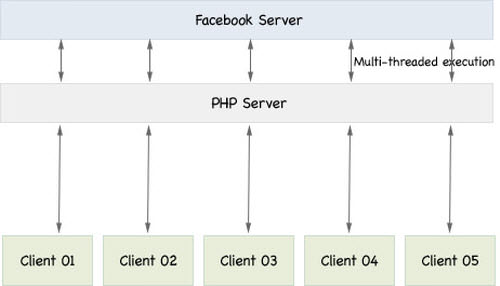
\includegraphics[width=0.7\textwidth]{multi-threaded.jpg}
	    \caption{Πολυνηματικό Μοντέλο.}
	    \label{fig:multi}
	\end{figure}
	
	
	
		 Ο πολυνηματισμός παρόλο που λύνει το πρόβλημα της απόδοσης και των μεγάλων νεκρών διαστημάτων της πρώτης υλοποίησης παρουσιάζει κάποια προβλήματα. Αρχικά απαιτεί πολύ χρόνο εργασίας από τον προγραμματιστή καθώς και τη χρήση εξειδικευμένων λύσεων συγχρονισμού των νημάτων, όπως κλειδώματα (locks) και σημαφόρους (semaphores), με σκοπό να μην πραγματοποιηθεί ταυτόχρονη πρόσβαση δύο νημάτων στο ίδιο σημείο της μνήμης, η οποία θα έχει ως αποτέλεσμα ασυνέπειες  \cite{silberschatz}. Τέτοιου είδους λάθη (bugs) δεν είναι πάντα εύκολο να προβλεφθούν και πολλές φορές συμβαίνουν τυχαία και είναι πολύ δύσκολος ο εντοπισμός τους. Ένα άλλο μειονέκτημα του μοντέλου του πολυνηματισμού είναι ότι το μοντέλο  δεν κλιμακώνει ιδιαίτερα καλά καθώς ο αριθμός των χρηστών αυξάνεται. Η διαχείριση όλων αυτών των νημάτων είναι ένα μεγάλο βάρος για το λειτουργικό σύστημα, τόσο λόγω των απαιτήσεων μνήμης, όσο και λόγω της εναλλαγής περιβάλλοντος λειτουργίας. Η εναλλαγή της ΚΜΕ ανάμεσα στα νήματα απαιτεί την αποθήκευση της κατάστασης του τρέχοντος νήματος και την επαναφορά της κατάστασης του προς εκτέλεσης νήματος. 
		
		 
		 Το Node για να αντιμετωπίσει όλα αυτά τα προβλήματα, υιοθετεί μία διαφορετική προσέγγιση δημιουργώντας μόνο ένα νήμα το οποίο χειρίζεται όλες τις λειτουργίες Ε/Ε. Με αυτόν τον τρόπο επιτυγχάνει υψηλά επίπεδα κλιμάκωσης, που μπορεί να φτάσουν τις ένα εκατομμύριο ταυτόχρονες συνδέσεις. Στο σχήμα \ref{fig:single} φαίνεται ένα παράδειγμα από το μονονηματικό μοντέλο του NodeJs.
		 
			 \begin{figure}[h]
	    \centering
	    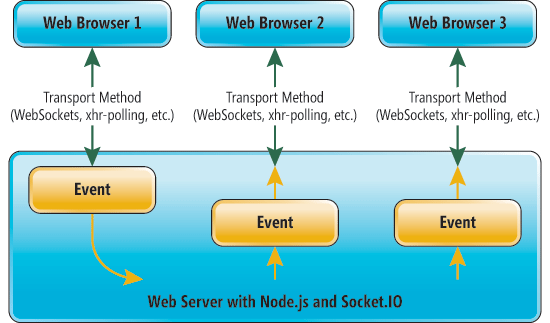
\includegraphics[width=0.7\textwidth]{single.png}
	    \caption{ Το μονονηματικό μοντέλο του NodeJs.}
	    \label{fig:single}
	\end{figure} 

\subsubsection{Event-driven model}		 

		O οδηγούμενος από τα γεγονότα (event-driven) προγραμματισμός είναι ένα προγραμματιστικό μοντέλο όπου η ροή της εκτέλεσης ``οδηγείται'' από γεγονότα. Τα γεγονότα αυτά τα χειρίζονται είτε οι επιστρεφόμενες κλήσεις των γεγονότων είτε οι χειριστές συμβάντος. Μια επιστρεφόμενη κλήση είναι μια συνάρτηση η οποία καλείται όταν συμβαίνει ένα συγκεκριμένο γεγονός. Στα πλαίσια του εξυπηρετητή το γεγονός στο οποίο αναφερόμαστε συνήθως αποτελεί η ολοκλήρωση μιας λειτουργίας Ε/Ε. Για παράδειγμα, σε μια γραφική διεπαφή χρήστη έχουμε ως γεγονότα τα πατήματα πλήκτρων ή επιλογών με το ποντίκι.
		
		Στις περιπτώσεις που οι λειτουργίες Ε/Ε επιστρέφουν μία συνάρτηση και όχι απλά μία τιμή έχουμε το μοντέλο του ασύγχρονου ή οδηγούμενου από γεγονότα προγραμματισμού. Έτσι επιτυγχάνεται η παραλληλοποίηση των Ε/Ε λειτουργιών,ενώ κάθε φορά η συνάρτηση επιστρεφόμενης κλήσης ενημερώνει για την ολοκλήρωση της αντίστοιχης λειτουργίας. Η JavaScript ανήκει σε αυτό το είδος προγραμματισμού. Η JavaScript υποστηρίζει επιπλέον το μοτίβο κλεισίματος (closure pattern) καθώς και το πέρασμα συναρτήσεων σαν παραμέτρους σε άλλη συνάρτηση (first-class functions).
		

		Ο οδηγούμενος από τα γεγονότα προγραμματισμός συνοδεύεται από έναν βρόχο γεγονότων (event loop). Ο βρόχος γεγονότων είναι ένα loop το οποίο σε κάθε επανάληψη ανιχνεύει γεγονότα και ενεργοποιεί τον αντίστοιχο χειριστή συμβάντος. Ουσιαστικά κοιτάει σε κάθε επανάληψη ποια λειτουργία Ε/Ε έχει ολοκληρωθεί και καλεί την αντίστοιχη συνάρτηση επιστρεφόμενης κλήσης. Ο βρόχος γεγονότων υλοποιείται από ένα νήμα μέσα σε μια διεργασία και με βάση όσα αναφέρθηκαν για τα νήματα εύκολα προκύπτει ότι κάθε χρονική στιγμή τρέχει το πολύ ένα νήμα, που στην περιπτωσή μας είναι ένας διαχειριστής γεγονότος, και ότι κάθε διαχειριστής γεγονότος τρέχει μέχρι να ολοκληρωθεί χωρίς διακοπή.
		
		\subsubsection{Ο Διαχειριστής Πακέτων του Node (Node Package Manager ,NPM)}
		

		Ο διαχειριστής πακέτων του Node (Node Package Manager ή NPM) παρέχει την δυνατότητα να κατεβάσουμε, να εγκαταστήσουμε και να τρέξουμε στην εφαρμογή μας πακέτα (modules) τρίτων. H εγκατάσταση του διαχειριστή  πακέτων πραγματοποιείται αυτόματα όταν εγκαθιστούμε την πλατφόρμα του Node. Μετά την εγκατάσταση του Node, έχουμε πρόσβαση σε κάποια ενσωματωμένα πακέτα, τα οποία μας παρέχουν κάποιες διεπαφές εφαρμογών χαμηλού επιπέδου (low-level APIs) ώστε να μπορούμε να υλοποιήσουμε κάποιες βασικές λειτουργίες που χρειάζονται οι εφαρμογές. Αυτά τα πακέτα ονομάζονται ως ο πυρήνας του NodeJs . Στα πλαίσια σύνθετων εφαρμογών είναι σχεδόν απαραίτητο να συμπεριλάβουμε πακέτα τρίτων.


		Το σύνολο όλων των πακέτων που έχουν φτιάξει και δημοσιοποιήσει οι προγραμματιστές διατηρείται σε μία κεντρική αποθήκη από τον διαχειριστή πακέτων του Node. Ο διαχειριστής πακέτων παρέχει ένα εργαλείο γραμμής-εντολών (command-line tool), όπου ο χρήστης μπορεί να εγκαθιστά και να διαχειρίζεται τα πακέτα αυτά. H αναζήτηση τέτοιων πακέτων μπορεί να πραγματοποιηθεί είτε μέσω της γραμμής εντολών είτε μέσω της σελίδας www.npmjs.org. Σε αυτήν την σελίδα παρουσιάζονται και διάφορα στατιστικά στοιχεία, όπως πόσα πακέτα υπάρχουν συνολικά, από ποια πακέτα εξαρτώνται περισσότερο άλλα πακέτα κ.λ.π. \cite{cantelon}		
				
	\subsubsection{Ο Εξυπηρετητής (Server)}
	
		To NodeJs κάνει την δημιουργία διαφόρων τύπων εξυπηρετητών (servers) μια πολύ εύκολη διαδικασία καθώς στο NodeJs ο εξυπηρετητής και η εφαρμογή είναι το ίδιο.

		
	\subsection{Βάση Δεδομένων}
	Στο παρόν κεφάλαιο κάνουμε μια σύντομη αναφορά στα διάφορα συστήματα βάσεων δεδομένων τύπου NoSQL, τα πλεονεκτήματα τους καθώς και τις εφαρμογές για τις οποίες ενδείκνυται η χρήση τους.
	
	Η ιδέα ενός συστήματος βάσης δεδομένων τύπου NoSQL παρουσιάστηκε για πρώτη φορά το 1998 χωρίς να προχωρήσει όμως ιδιαίτερα και επανήλθε πάλι στο προσκήνιο το 2009, όταν και αναπτύχθηκαν αρκετές NoSQL λύσεις \cite{5993686} \cite{Codd:1970:RMD:362384.362685}. Η διαδικασία απόδοσης κάποιου συγκεκριμένου ορισμού για τον όρο NoSQL δεν αποτελεί απλή διαδικασία, δεδομένου ότι δεν αναφέρεται σε ένα συγκεκριμένο σύστημα διαχείρισης βάσεων δεδομένων, αλλά αποτελεί έναν γενικό όρο που περικλείει πολλά συστήματα βάσεων δεδομένων.
	
	Στον τομέα της επιστήμης των υπολογιστών όταν αναφερόμαστε στον όρο NoSQL (Not Only SQL), μιλάμε για ένα ευρύ φάσμα συστημάτων διαχείρισης βάσεων δεδομένων τα οποία παρέχουν ένα μηχανισμό προς αποθήκευση και ανάκτηση δεδομένων διαφορετικό από αυτό του σχεσιακού μοντέλου των κλασσικών RDBMS (Relational database management system)\cite{Cattell:2011:SSN:1978915.1978919}\cite{6106531}. Τα συστήματα NoSQL ξεφεύγουν από την παραδοσιακή χρήση πινάκων για την οργάνωση των δεδομένων και χρησιμοποιούν διαφορετικές δομές οργάνωσης, όπως αυτή του κλειδιού-τιμής. Επιπροσθέτως η επεξεργασίά αυτών των δεδομένων δεν γίνεται με χρήση ερωτημάτων SQL όπως έχουμε συνηθίσει. Λόγω των εγγενών διαφορών μεταξύ των δύο αυτών συστημάτων, κάποιες λειτουργίες είναι ταχύτερες στα συστήματα NoSQL ενώ κάποιες άλλες στα συστήματα σχεσιακών βάσεων δεδομένων.
	
	\begin{figure}[h]
	    \centering
	    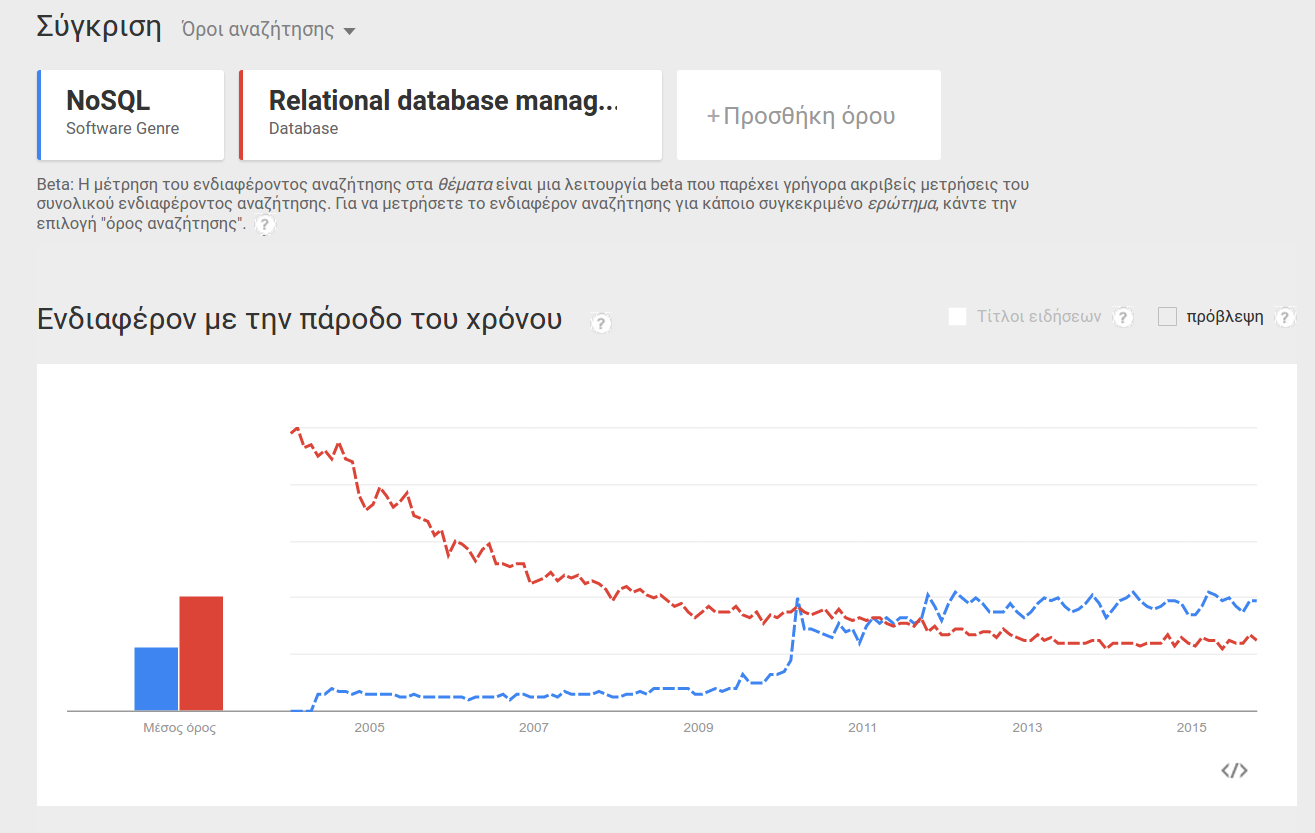
\includegraphics[width=1\textwidth]{nosql_vs_rdbms.png}
	    \caption{Τάση αναζητήσεων Google για NoSQL σε σύγκριση με RDBMS.}
	    \label{fig:NoSQL_vs_rdbms_google}
	\end{figure}
	
	Η χρήση των βάσεων δεδομένων τύπου NoSQL έχει γνωρίσει ραγδαία αύξηση τα τελευταία χρόνια σε εφαρμογές big data καθώς και σε εφαρμογές πραγματικού χρόνου. Αποκαλούνται με τον όρο Not Only SQL για να δοθεί έμφαση στο γεγονός ότι οι δύο τεχνολογίες δεν είναι αμοιβαία αποκλειόμενες. Έχουν τη δυνατότητα να συνυπάρχουν, κρατώντας τα δυνατά σημεία της κάθε μιας, προσφέροντας σε διαφορετικές καταστάσεις διαφορετικές υπηρεσίες. Οι βάσεις δεδομένων τύπου NoSQL χρησιμοποιούνται από εταιρείες κολοσσούς του τεχνολογικού τομέα όπως το Facebook, Amazon, Google, LinkedIn\cite{5993686}. Ο όγκος των δεδομένων που διαχειρίζονται τέτοιες εταιρείες είναι της τάξης πολλών petabyte και επομένως θα ήταν αδύνατη η κλιμάκωσή τους με κάποιο σχεσιακό σύστημα ΒΔ. Κι αυτό γιατί οι σχεσιακές ΒΔ συναντούν περιορισμούς όσον αφορά την αντιμετώπιση προβλημάτων όπως είναι η εξόρυξη δεδομένων, το Web 2.0, το cloud computing, τα μη γραμμικά σε εκτέλεση ερωτήματα κ.τ.λ.
	
	\begin{figure}[h]
	    \centering
	    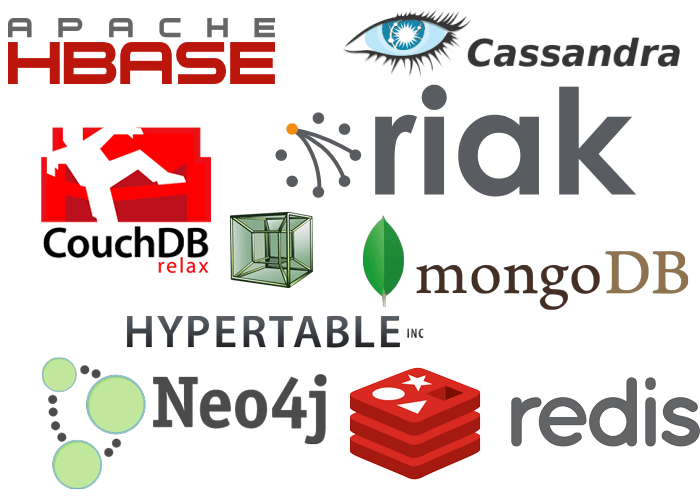
\includegraphics[width=0.7\textwidth]{NoSQL-DBs.png}
	    \caption{Δημοφιλές βάσεις δεδομένων τύπου NoSQL.}
	    \label{fig:NoSQL-DBs}
	\end{figure}
	
	Τα NoSQL συστήματα δεν εμφανίστηκαν για να αντικαταστήσουν τα σχεσιακά, αλλά για να τα συμπληρώσουν. Όπως και σε πολλές άλλες περιπτώσεις έτσι και εδώ, το ζητούμενο είναι να γίνει η επιλογή του κατάλληλου εργαλείου για τη λύση του κάθε προβλήματος. Έτσι στις περισσότερες περιπτώσεις είναι απαραίτητο να γίνει μια εκτίμηση των δυνατοτήτων των διαθέσιμων συστημάτων και στη συνέχεια να υλοποιηθεί ένας συνδυασμός τους ώστε κάθε επιμέρους ανάγκη να καλύπτεται από το σύστημα που της ταιριάζει καλύτερα. Έτσι, όσο τα δεδομένα του διαδικτύου αυξάνονται με εκθετικούς ρυθμούς, τόσο πιο πολλές θα είναι και οι περιπτώσεις όπου θα καθίσταται καλή επιλογή η χρήση τους. Η ανάπτυξη των NoSQL συστημάτων είναι πολύ γρήγορη τα τελευταία χρόνια. Τη στιγμή της συγγραφής της παρούσας διπλωματικής εργασίας, η λίστα με τις NoSQL βάσεις δεδομένων περιλαμβάνει περίπου 225 καταχωρήσεις όταν πριν από τέσσερα χρόνια οι καταχωρήσεις έφταναν τις 35\cite{numberOfNoSQL}.
		
		\subsubsection{Τύποι NoSQL}
		Όπως αναφέραμε και προηγουμένως με τον όρο NoSQL αναφερόμαστε σε ένα ευρύ φάσμα τεχνολογιών. Στην παρούσα ενότητα θα κάνουμε μια σύντομη παρουσίαση των πιο διαδεδομένων τεχνολογιών.
		
		\subsubsection{Key-value Stores (Αποθήκες κλειδιών-τιμών)}
		Το μοντέλο κλειδιού - τιμής είναι το πιο απλό από όλες τις κατηγορίες που εξετάζουμε. Τα δεδομένα αποθηκεύονται σε ζεύγη κλειδιού - τιμής, με τρόπο παρόμοιο με μία απεικόνιση (map) ή με έναν πίνακα κατακερματισμού (hash table). Κάποια συστήματα μπορεί να επιτρέπουν η τιμή να είναι κάτι πιο πολύπλοκο, όπως για παράδειγμα μία λίστα. Αποτελούν ουσιαστικά αποθήκες δεδομένων, οι οποίες λειτουργούν με τη χρήση ενός hashtable, στο οποίο αποθηκεύονται μοναδικά κλειδιά και δείκτες για τα δεδομένα του κάθε αντικειμένου. Τέτοιου τύπου αποθήκες δεδομένων προσφέρουν υπηρεσίες για τη διαχείριση δεδομένων χωρίς τον ορισμό συγκεκριμένου σχήματος. Το γεγονός ότι το μοντέλο είναι τόσο απλό, κάνει τις βάσεις αυτού του είδους να πετυχαίνουν πολύ καλές επιδόσεις όταν η συγκεκριμένη δομή ταιριάζει στο πρόβλημα. Τα δεδομένα για να είναι κατάλληλα για μια τέτοια βάση, δεν θα πρέπει να έχουν υψηλά επίπεδα συσχετίσεων μεταξύ τους. Αν το ζητούμενο είναι να υπάρχει δυνατότητα για πολύπλοκα ερωτήματα στη βάση, τότε το μοντέλο αυτό δεν διευκολύνει. Από τα πιο γνωστά συστήματα που ανήκουν σε αυτή την κατηγορία είναι τα memcached, membase, cachedb, Voldemort, Scalaris, Dynamo, Redis και Riak\cite{DeCandia:2007:DAH:1323293.1294281}\cite{seeger2009key}.
		
		\subsubsection{Column-oriented Databases (Βάσεις δεδομένων προσανατολισμένες στη στήλη)}
		Δημιουργήθηκαν με σκοπό την αποθήκευση και την επεξεργασία μεγάλης ποσότητας δεδομένων, τα οποία είναι κατανεμημένα σε πολλούς διαφορετικούς υπολογιστικούς κόμβους. Υπάρχουν και στην περίπτωση αυτή κλειδιά το οποία δείχνουν σε διαφορετικά σύνολα στηλών. Οι γραμμές διαχωρίζονται από κλειδιά και οι στήλες χωρίζονται σε οικογένειες. Οι column-oriented βάσεις δεδομένων από άποψη δομής βρίσκονται κάπου ανάμεσα στους σχεσιακούς πίνακες και στο μοντέλο κλειδιού - τιμής. Θα μπορούσαμε να πούμε ότι αποτελούνται από πίνακες οι οποίοι όμως διαφέρουν από τους παραδοσιακούς των σχεσιακών βάσεων ως προς τον τρόπο με τον οποίο αποθηκεύουν τα δεδομένα. Η διαφορά βρίσκεται στο ότι στους πίνακες κατά στήλες, τα δεδομένα από μία στήλη αποθηκεύονται μαζί στον δίσκο (σε αντίθεση με τους πίνακες των σχεσιακών βάσεων που αποθηκεύονταν κατά γραμμές). Αυτή η αλλαγή, παρ' ότι φαίνεται μικρή δημιουργεί πολύ διαφορετικές συνθήκες και ιδιότητες στο σύστημα. Η προσθήκη επιπλέον στηλών είναι μια διαδικασία που δεν κοστίζει, κάθε γραμμή μπορεί να έχει διαφορετικές στήλες ή και καθόλου, και επίσης οι πίνακες μπορούν να παραμένουν αραιοί χωρίς αυτό όμως να έχει επίπτωση στον αποθηκευτικό χώρο που απαιτούν.
		
	\begin{figure}[h]
	    \centering
	    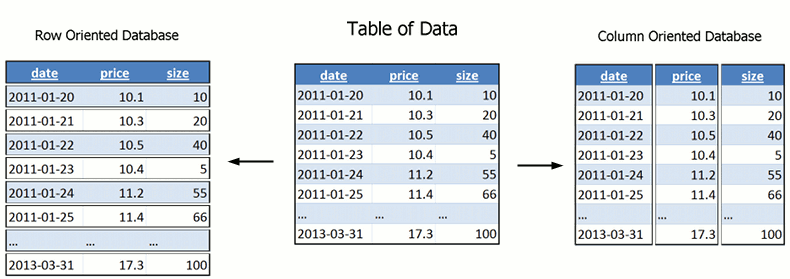
\includegraphics[width=0.8\textwidth]{column-vs-row-oriented-database.png}
	    \caption{Αποθήκευση κατά Σειρές και κατά Στήλες.}
	    \label{fig:column-oriented-dbs}
	\end{figure}
	
	Ένα σημαντικό χαρακτηριστικό που έχουν τέτοια συστήματα είναι οι ενσωματωμένες δυνατότητες για συμπίεση των δεδομένων, αφού η οργάνωση κατά στήλες κάνει τα δεδομένα που βρίσκονται σε μία στήλη να είναι όμοια και έτσι οι αλγόριθμοι συμπίεσης πετυχαίνουν καλύτερα αποτελέσματα. Το χαρακτηριστικό αυτό γίνεται πολύ σημαντικό όταν ο όγκος των δεδομένων είναι μεγάλος. Είναι γενικά καλό με τις συγκεκριμένες βάσεις να υπάρχει ένα πλάνο για το πώς θα χρησιμοποιηθούν τα δεδομένα και τι ερωτήματα θα γίνονται σε αυτά, έτσι ώστε να γίνει κατάλληλη επιλογή της δομής των δεδομένων και να είναι αποδοτική η βάση στη συνέχεια. Αν δεν είναι δυνατόν να γίνει μία τέτοια εκτίμηση εκ των προτέρων, τότε τα συγκεκριμένα συστήματα μπορεί να μην αναδεικνύουν τα δυνατά τους χαρακτηριστικά. Παραδείγματα τέτοιων συστημάτων βάσεων δεδομένων είναι τα BigTable, Cassandra, Hyperbase και HBase\cite{abadi2006integrating}\cite{abadi2009column}.
	
		\subsubsection{Document-oriented Databases (Βάσεις δεδομένων βασισμένες στα έγγραφα)}
		Οι βάσεις οργανωμένες κατά αρχεία, όπως λέει και το όνομά τους, χρησιμοποιούν αρχεία για να αποθηκεύσουν τα δεδομένα. Τα αρχεία αυτά έχουν ένα μοναδικό αναγνωριστικό ID το καθένα και συνήθως η βάση διατηρεί ευρετήριο (index) ώστε να γίνεται γρήγορα η αναζήτηση και η ανάκτηση τους. Σαν τιμή μπορεί να περιέχουν κάθε είδους δεδομένα με μοναδικό περιορισμό να μπορούν να εκφραστούν σαν αρχείο, γεγονός που παρέχει μεγάλη ευελιξία. Τα αρχεία είναι συνήθως τύπου JSON (JavaScript Object Notation) είτε παραλλαγές όπως BSON (Binary JSON) τα οποία είναι κατάλληλα τόσο για την μεταφορά και την αποθήκευση, όσο και για την ανάγνωση και τον χειρισμό των δεδομένων, αφού είναι ένα πρότυπο με το οποίο τα δεδομένα περιγράφουν από μόνα τους τη δομή τους, χωρίς αυτό να προσθέτει κάποιο περιορισμό στη βάση. Λόγω της φύσης των αρχείων, συνήθως τέτοιου είδους συστήματα ταιριάζουν με αντικειμενοστραφείς γλώσσες προγραμματισμού. Μία ιδιαιτερότητα των βάσεων που οργανώνονται κατά αρχεία είναι ότι τα δεδομένα κατά βάση δεν είναι κανονικοποιημένα όπως στις σχεσιακές βάσεις, αλλά κάθε αρχείο προβλέπεται να διατηρεί τις περισσότερες αν όχι όλες τις πληροφορίες που μπορεί να χρειαστούν όταν πραγματοποιείται η ενέργεια που το αφορά. Παραδείγματα τέτοιων συστημάτων βάσεων δεδομένων είναι τα MongoDB, CouchDB, Couchbase, RethinkDB, Terrastore, Elasticsearch\cite{banker2011mongodb}\cite{redmond2012seven}.
		
	\begin{figure}[h]
	    \centering
	    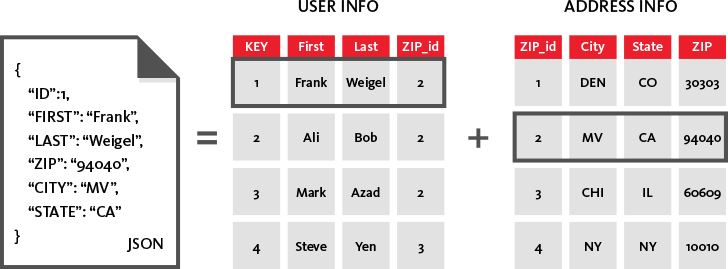
\includegraphics[width=0.7\textwidth]{document_oriented_db.png}
	    \caption{Βάσεις δεδομένων βασισμένες στα έγγραφα.}
	    \label{fig:document_oriented_db}
	\end{figure}
		
		\subsubsection{Graph databases (Βάσεις δεδομένων γράφου)}
		Βασίζονται στη θεωρία των γράφων για την κατασκευή συστημάτων με κόμβους, οι οποίοι τοποθετούνται ανάλογα με τις σχέσεις που προκύπτουν μεταξύ των δεδομένων. Οι βάσεις δεδομένων αυτής της κατηγορίας δεν χρησιμοποιούνται συχνά, αφού είναι κατάλληλη επιλογή μόνο σε περιπτώσεις οπού τα δεδομένα παρουσιάζουν μεγάλη συσχέτιση μεταξύ τους και η συσχέτιση αυτή πρέπει να αποτυπωθεί. Μοντελοποιούνται με κόμβους και με σχέσεις που τους συνδέουν. Χαρακτηριστική λειτουργία σε τέτοιου είδους βάσεις είναι να διασχίζονται οι κόμβοι χρησιμοποιώντας τις σχέσεις που τους συνδέουν. Τέλος, οι κόμβοι και οι σχέσεις μπορούν να έχουν ιδιότητες στις οποίες αποθηκεύονται δεδομένα. Η κλασσική χρήση τέτοιων συστημάτων είναι σε κοινωνικά δίκτυα, όπου οι σχέσεις μεταξύ των χρηστών είναι πολλές και πολύπλοκες. Σε τέτοιες περιπτώσεις τα υπόλοιπα συστήματα βάσεων δεδομένων ταιριάζουν αρκετά λιγότερο και προσθέτουν δυσκολίες. Το γεγονός όμως ότι οι εξαρτήσεις μεταξύ των δεδομένων είναι τόσο πολλές, καθιστά δύσκολο το να γίνουν αυτά τα συστήματα κατανεμημένα, αφού σε περίπτωση κατάτμησης λόγω δικτύου οι σχέσεις που δεν θα είναι πλέον προσβάσιμες μπορεί να είναι πάρα πολλές. Παράδειγμα τέτοιων συστημάτων είναι τα Neo4j, AllegroGraph, GraphDB, FlockDB, OrientDB\cite{he2008graphs}\cite{robinson2013graph}.
		
		\subsubsection{Object-oriented databases (Αντικειμενοστραφείς βάσεις)}
		Οι αντικειμενοστρεφείς βάσεις δεδομένων αποθηκεύουν τα δεδομένα τους, όπως υποδεικνύει το όνομά τους με τη μορφή αντικειμένων, όπως αυτά χρησιμοποιούνται στις αντικειμενοστρεφείς γλώσσες προγραμματισμού. Αυτό κάνει πιο άμεση και απλή τη χρησιμοποίησή τους από εφαρμογές γραμμένες σε τέτοιου είδους γλώσσες, αφού δε χρειάζεται η χρήση επιπλέον κώδικα για την αντιστοίχιση των δεδομένων με την εφαρμογή. Το γεγονός ότι δε χρειάζεται κάποια μετάφραση των αντικειμένων που χρησιμοποιούνται, σε κάποια άλλη μορφή (πχ κατάλληλη για σχεσιακές βάσεις), κάνει τις αντικειμενοστρεφείς βάσεις να παρουσιάζουν συχνά αυξημένη επίδοση σε σχέση με άλλα συστήματα. Επίσης δεν είναι απαραίτητη η δημιουργία κλειδιών για να επιτευχθεί η συσχέτιση και η αντιστοίχιση των δεδομένων, τα οποία μπορούν να αναζητηθούν με τη χρήση δεικτών (pointers).
		
		Οι αντικειμενοστρεφείς βάσεις δεδομένων έχουν εμφανιστεί από τα μέσα της δεκαετίας του 70 και βρήκαν ανταπόκριση σε κάποιες εφαρμογές όπως CAD (Computer Aided Design), CAM (Computer Aided Manufacturing) και σε ενσωματωμένα συστήματα, όμως ποτέ δεν έγινε εκτεταμένη χρήση τους. Αυτό οφείλεται σε κάποια μειονεκτήματα που παρουσιάζουν σε σχέση με άλλα συστήματα. Το κυριότερο από αυτά είναι ότι η βάση που δημιουργείται συσχετίζεται στενά με την εφαρμογή που τη χρησιμοποιεί και πιθανώς και με τη γλώσσα στην οποία είναι γραμμένη η εφαρμογή. Αυτό κάνει τη βάση λιγότερο ευέλικτη σε σχέση με άλλες εναλλακτικές. Επίσης για απλές περιπτώσεις βάσεων που περιέχουν απλές σχέσεις, οι αντικειμενοστρεφείς βάσεις μπορεί να είναι λιγότερο αποδοτικές και πιο πολύπλοκες σε σχέση με ένα σύστημα RDBMS. Παράδειγμα τέτοιων συστημάτων είναι τα VelocityDB, Versand, Objectivity, Starcounter, Perst, HSS Database, Sterling\cite{bertino1997object}\cite{kim1990introduction}\cite{kim2014object}\cite{leavitt2000whatever}.
		
		\subsubsection{Χαρακτηριστικά NoSQL βάσεων δεδομένων}
		
		\subsubsection{Ανθεκτικότητα}
		Όπως και στις σχεσιακές βάσεις, έτσι και στις NoSQL βάσεις όταν κάτι γραφτεί στο δίσκο είμαστε σίγουροι πως δε θα χαθεί. Η διαφορά από τις σχεσιακές βάσεις βέβαια είναι πως στα κατανεμημένα συστήματα κάτι τέτοιο σημαίνει πως η πληροφορία έχει γραφτεί εκ προεπιλογής σε παραπάνω από έναν δίσκο και επομένως δε θα χαθεί ακόμα και σε περίπτωση αποτυχίας ενός δίσκου ή υπολογιστή\cite{schindler2012characteristics}\cite{stonebraker2010sql}.
		
		\subsubsection{Προσαρμοστικότητα}
		Οι NoSQL βάσεις είναι ευέλικτες σχετικά με τα δεδομένα που αποθηκεύουν. Δεν υπάρχει περιορισμός στον τύπο των δεδομένων που μπορούν να αποθηκευτούν, ενώ στις SQL βάσεις ο τύπος έχει καθοριστεί κατά τη δημιουργία τους. Ακόμη, οι NoSQL βάσεις μπορούν να αντιμετωπίσουν με ευκολία πιο πολύπλοκες και προηγμένες δομές δεδομένων. Οι περισσότερες από τις υπάρχουσες NoSQL βάσεις, παρέχουν πλούσιες δομές δεδομένων και εργασιών σε λίστες, σύνολα, ταξινομημένα σύνολα και κλειδιά κατακερματισμού που κάνουν πράγματα όπως εξισορρόπηση φορτίου και message-queuing απλούστατα στην υλοποίηση\cite{stonebraker2010sql}\cite{grazioli2014mapping}.
		
		\subsubsection{Διαχειρισιμότητα}
		Η ύπαρξη ενός άριστα εκπαιδευμένου, με πολλή εμπειρία και γνώση, διαχειριστή βάσεων δεδομένων είναι απαραίτητη για τη συντήρηση ενός υψηλού επιπέδου RDBMS. Είναι άρρηκτα συνδεδεμένος με όλες τις λειτουργίες που αφορούν τη βάση, δηλαδή με το σχεδιασμό, την εγκατάσταση και τη συνεχή παρακολούθηση και ρύθμιση της. Οι μη σχεσιακές βάσεις από τα θεμέλιά τους έχουν σχεδιαστεί για να χρειάζονται λιγότερη διαχείριση. Η δυνατότητα αυτόματης επισκευής, η διανομή δεδομένων, το απλούστερο μοντέλο δεδομένων είναι όλα χαρακτηριστικά που συντελούν στη μείωση των απαιτήσεων σε θέματα ρύθμισης και διαχείρισης\cite{stonebraker2010sql}.
		
		\subsubsection{Παράλληλη επεξεργασία}
		Χάρη στις δυνατότητες που προσφέρουν τα συστήματα NoSQL, όπως εύκολη αναπαραγωγή και διαμοιρασμός δεδομένων, καθίσταται εξίσου εύκολη και η εκμετάλλευση των φυσικών πόρων του συμπλέγματος όπου λειτουργεί η βάση. Από τη στιγμή που τα δεδομένα βρίσκονται σε διαφορετικούς δίσκους, υπολογιστές ή ακόμα και δίκτυα, τα ερωτήματα μπορούν χωρίς καθόλου επιπλέον κώδικα να εκτελούνται παράλληλα και να δίνουν άμεσα απαντήσεις\cite{stonebraker2010sql}.
		
		\subsubsection{Διαθεσιμότητα}
		Όπως θα ήταν αναμενόμενο, δε συμφέρει καθόλου κάποια web ή mobile based επιχείρηση (π.χ. facebook) να είναι πεσμένη. Θέλει δηλαδή να υπάρχει όσο το δυνατόν λιγότερο downtime. Χάρη πάλι στο γεγονός ότι οι NoSQL βάσεις είναι κατανεμημένες, οι ενημερώσεις λογισμικού, αναβαθμίσεις υλικού αλλά και τυχόν αποτυχίες υλικού δε σημαίνουν πως θα πέσει η εφαρμογή, αφού υπάρχει σε πολλαπλούς servers. Αντιθέτως, αν η εφαρμογή βασίζεται σε μία σχεσιακή βάση, τα παραπάνω ισοδυναμούν με δυσκολίες και downtime\cite{stonebraker2010sql}.
		
		\subsubsection{Υψηλή απόδοση}
		Εκτός από το γεγονός ότι με την προσθήκη υπολογιστών στο cluster έχουμε ήδη περισσότερη υπολογιστική ισχύ και άρα καλύτερη απόδοση, η ίδια η αρχιτεκτονική των NoSQL εργαλείων κάνει τις βάσεις αυτές πιο αποδοτικές. Αν μία σχεσιακή βάση είχε μερικές εκατοντάδες χιλιάδες πίνακες, η επεξεργασία των δεδομένων θα δημιουργούσε πάρα πολλά locks και θα υποβάθμιζε την απόδοση. Λόγω όμως της ασθενέστερης συνέπειας που χαρακτηρίζει τα μοντέλα δεδομένων των NoSQL βάσεων, δίνεται βάρος στην αποτελεσματικότητα αντί της συνοχής και επομένως δεν υπάρχει πρόβλημα όσο μεγάλη και να είναι η βάση\cite{stonebraker2010sql}.
		
		\subsubsection{Αναπαραγωγή δεδομένων}
		Τα δεδομένα διανέμονται μεταξύ πολλών κόμβων με πολύ εύκολο τρόπο. Σε όλα τα NoSQL συστήματα κάτι τέτοιο ρυθμίζεται πολύ απλά βάζοντας σε ένα .conf αρχείο την ip ή το domain name των servers στους οποίους θέλουμε να αναπαράγονται τα δεδομένα. Η αυτοματοποίηση της αναπαραγωγής έχει ως αποτέλεσμα την υψηλή διαθεσιμότητα των δεδομένων και επομένως την εύκολη αποκατάσταση από καταστροφή τους, χωρίς να εμπλέκονται ξεχωριστές εφαρμογές για το σκοπό αυτό. Ακόμη, χάρη σε αυτό το χαρακτηριστικό, η προσθήκη ή αφαίρεση υλικού (υπολογιστές, servers κλπ) γίνεται χωρίς downtime\cite{stonebraker2010sql}.
		
		\subsubsection{Schema-less persistence – Δυναμικά Schemas}
		Στις σχεσιακές βάσεις είναι απαραίτητο το σχήμα να είναι ορισμένο πριν αρχίσουμε να προσθέτουμε δεδομένα. Για παράδειγμα, αν θέλουμε να κρατάμε σε κάποια SQL βάση  90 δεδομένα όπως όνομα, επώνυμο και τηλέφωνο πελάτη, είναι απαραίτητο η βάση αυτή να το γνωρίζει από πριν.
		
		Τώρα όμως που ο ρυθμός αύξησης των δυνατοτήτων ιστοσελίδων/εφαρμογών είναι ταχύτατος, κάθε φορά που ολοκληρώνεται κάποιο νέο χαρακτηριστικό, είναι πολύ πιθανό να χρειάζεται αλλαγή και το σχήμα της βάσης. Αν θέλω δηλαδή στη βάση του παραδείγματος να ξεκινήσω να κρατάω και κάτι παραπάνω για τους πελάτες, πρέπει να αλλάξω το σχήμα και να προσθέσω στήλη και ίσως να φτιάξω επιπλέον indexes/foreign keys κλπ. Αν η βάση είναι μεγάλη, η διαδικασία αυτή θα πάρει πολλή ώρα οπότε η βάση δε θα λειτουργεί για το διάστημα αυτό. Επίσης, με ένα σχεσιακό σύστημα, δεν υπάρχει τρόπος να αντιμετωπίσουμε δεδομένα που είναι αδόμητα ή άγνωστα από πριν. Επομένως, το φλέγον θέμα της διαχείρισης των αλλαγών (change management) είναι μεγάλος πονοκέφαλος σε ένα μεγάλο RDBMS.
		
		Αντιθέτως, οι NoSQL βάσεις είναι πολύ ευέλικτες και έχουν χαλαρούς (ή και ανύπαρκτους) περιορισμούς όσον αφορά στο μοντέλο δεδομένων. Είναι σχεδιασμένες να επιτρέπουν την εισαγωγή δεδομένων χωρίς την ύπαρξη προκαθορισμένου σχήματος. Έτσι, οι σημαντικές αλλαγές που χρειάζονται γίνονται σε πραγματικό χρόνο, χωρίς την ανησυχία για διακοπή της λειτουργίας της βάσης. Επομένως, η ανάπτυξη καθίσταται γρηγορότερη, η ενσωμάτωση κώδικα πιο αξιόπιστη και χρειάζεται λιγότερη ώρα ενασχόλησης του διαχειριστή της βάσης\cite{stonebraker2010sql}.
		
		\subsubsection{Κλιμάκωση}
		Είναι ίσως το πιο σημαντικό χαρακτηριστικό των NoSQL βάσεων. Όταν οι επισκέψεις σε ένα site γίνονται μερικές εκατοντάδες ή και χιλιάδες το δευτερόλεπτο, μία σχεσιακή βάση θα έπρεπε να είναι διαμοιρασμένη και αναπαραγμένη σε μεγάλο βαθμό για να καταφέρει να ανταποκριθεί. Μία NoSQL βάση όμως, λόγω της κατανεμημένης της φύσης, το μόνο που χρειάζεται για σωστή κλιμάκωση, είναι προσθήκη υπολογιστών στο σύμπλεγμα (cluster). Δε χρειάζεται ούτε σπατάλη του χρόνου του διαχειριστή της βάσης, ούτε πολύπλοκος κώδικας για partitioning και replication. Ιδιαίτερα με τις νέες τεχνολογίες του cloud και των virtual machines, η κλιμάκωση είναι ιδιαίτερα εύκολη και φθηνή λύση\cite{stonebraker2010sql}. Σε αυτό το σημείο θα πρέπει να αναφερθεί ότι για την κλιμάκωση μιας βάσης δεδομένων υπάρχουν δύο επιλογές α)κατακόρυφη, β)οριζόντια κλιμάκωση. Κατακόρυφη σημαίνει να αυξάνονται συνεχώς οι δυνατότητες των υπαρχόντων εξυπηρετητών ενώ οριζόντια σημαίνει απλά προσθήκη υπολογιστών στο σύμπλεγμα όπως αναφέρθηκε και παραπάνω.
		
		\begin{itemize}
			\item {\textbf{Κατακόρυφη κλιμάκωση}}\\
			Στο επίπεδο της εφαρμογής της αρχιτεκτονικής διαδικτύου τριών επιπέδων, η οριζόντια κλιμάκωση ήταν η προεπιλεγμένη λύση για πολλά χρόνια και λειτουργούσε πολύ καλά. Καθώς όλο και περισσότεροι άνθρωποι χρησιμοποιούν μια εφαρμογή, περισσότεροι εξυπηρετητές του εμπορίου προστίθενται στο επίπεδο της εφαρμογής, η απόδοση διατηρείται με την κατανομή του φόρτου εργασίας σε ένα αυξημένο αριθμό εξυπηρετητών και το κόστος κλιμακώνεται γραμμικά σε σχέση με τον αριθμό των χρηστών
			
	\begin{figure}[h]
	    \centering
	    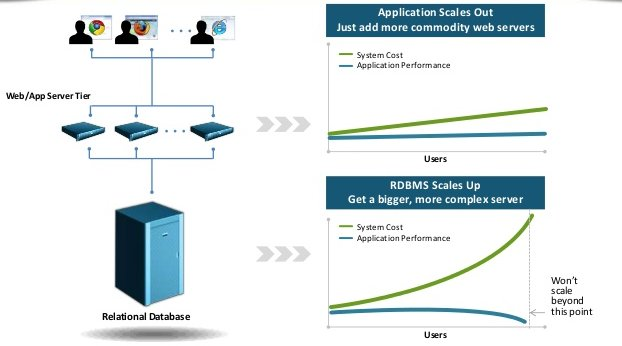
\includegraphics[width=1\textwidth]{RDBMS_scales_up.jpg}
	    \caption{Κλιμακωσιμότητα RDBMS.}
	    \label{fig:RDBMS_scales_up}
	\end{figure}	
			
			Πριν από τις NoSQL βάσεις δεδομένων, η προεπιλεγμένη προσέγγιση ως προς την κλιμάκωση στο επίπεδο της βάσης δεδομένων ήταν η κατακόρυφη κλιμάκωση. Αυτό υπαγορευόταν από τη θεμελιωδώς συγκεντρωτική αρχιτεκτονική της σχεσιακής τεχνολογίας βάσεων δεδομένων. Για την υποστήριξη περισσότερων ταυτόχρονων χρηστών και/ή την αποθήκευση περισσότερων δεδομένων, χρειάζονται όλο και υψηλότερων δυνατοτήτων εξυπηρετητές με περισσότερους επεξεργαστές, περισσότερη μνήμη και περισσότερο αποθηκευτικό χώρο για όλους τους πίνακες. Οι μεγάλοι εξυπηρετητές τείνουν να είναι πολύ πολύπλοκοι, ιδιοταγείς και δυσανάλογα ακριβοί εν αντιθέσει με αυτούς του εμπορίου.	
				
		\item {\textbf{Οριζόντια κλιμάκωση}}\\		
		Οι NoSQL βάσεις δεδομένων αναπτύχθηκαν εξ αρχής ώστε να είναι κατανεμημένες και να ευνοούν την οριζόντια κλιμάκωση. Χρησιμοποιούν ένα σύμπλεγμα τυπικών, φυσικών ή εικονικών εξυπηρετητών για να αποθηκεύουν δεδομένα και να υποστηρίζουν τις λειτουργίες της βάσης δεδομένων. Για κλιμάκωση, επιπλέον εξυπηρετητές προστίθενται στο σύμπλεγμα και τα δεδομένα και οι λειτουργίες της βάσης δεδομένων μοιράζονται στο μεγαλύτερο σύμπλεγμα. Επίσης, επειδή οι εξυπηρετητές του εμπορίου αναμένεται να παρουσιάσουν σφάλματα ανά κάποια χρονικά διαστήματα, οι βάσεις δεδομένων NoSQL έχουν δημιουργηθεί έτσι ώστε να είναι ανεκτικές και να ανακάμπτουν από τέτοια προβλήματα και αυτό τις καθιστά πολύ ανθεκτικές. Οι NoSQL βάσεις δεδομένων παρέχουν μια πολύ ευκολότερη και γραμμική προσέγγιση στην κλιμάκωση των βάσεων δεδομένων. Για κάθε 10,000 νέους χρήστες που αρχίζουν να χρησιμοποιούν μια εφαρμογή, τότε πρέπει απλά να προστεθεί μια ένας νέος εξυπηρετητής βάσης δεδομένων στο σύμπλεγμα. Με αυτόν τον τρόπο η εφαρμογή δεν χρειάζεται τροποποίηση καθώς αυτή βλέπει συνέχεια μόνο μια (κατανεμημένη) βάση δεδομένων.
		
	\begin{figure}[h]
	    \centering
	    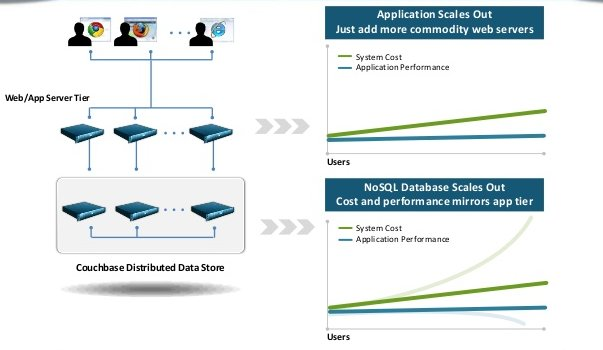
\includegraphics[width=1\textwidth]{nosql_scales_out.jpg}
	    \caption{Κλιμακωσιμότητα NoSQL.}
	    \label{fig:nosql_scales_out}
	\end{figure}
	
	Μια κατανεμημένη προσέγγιση οριζόντιας κλιμάκωσης επίσης συνήθως καταλήγει να είναι φθηνότερη από την εναλλακτική κατακόρυφης κλιμάκωσης. Αυτό είναι συνέπεια του ότι οι μεγάλοι, πολύπλοκοι και ανεκτικοί στα σφάλματα εξυπηρετητές έχουν υψηλά κόστη σχεδιασμού, κατασκευής και συντήρησης. Τα κόστη των αδειών των εμπορικών σχεσιακών βάσεων δεδομένων μπορεί επίσης να είναι απαγορευτικά, λόγω του ότι κοστολογούνται θεωρώντας ότι θα χρησιμοποιηθεί ένας μόνο εξυπηρετητής. Από την άλλη, οι βάσεις δεδομένων NoSQL είναι γενικά ανοιχτού κώδικα και κοστολογούνται με βάση το ότι θα χρησιμοποιηθούν σε ένα σύμπλεγμα εξυπηρετητών και είναι περισσότερο οικονομικές.		
		
		\end{itemize}
		
		\subsubsection{Ενσωματωμένο caching}
		Οι περισσότερες NoSQL βάσεις παρέχουν τεχνολογίες ενσωματωμένου caching. Τα συχνά χρησιμοποιούμενα δεδομένα αποθηκεύονται στη μνήμη όσο το δυνατόν περισσότερο και επομένως η επικοινωνία με το δίσκο ελαχιστοποιείται. Έτσι δεν υπάρχει η ανάγκη για ξεχωριστό επίπεδο caching, ενώ στις περισσότερες SQL βάσεις χρειάζεται ξεχωριστή υποδομή για να επιτευχθεί κάτι τέτοιο\cite{stonebraker2010sql}.
		
		\subsubsection{Μικρότερο κόστος}
		Στις NoSQL βάσεις χρησιμοποιούνται φθηνοί, απλοί servers που μπορεί να βρίσκονται και στο cloud ή να είναι εικονικοί. Από την άλλη, τα RDBMS βασίζονται σε ακριβούς, ιδιωτικούς servers και συστήματα αποθήκευσης. Το κόστος gb ή δοσοληψία ανά δευτερόλεπτο είναι επομένως πολύ χαμηλότερο σε ένα σύστημα NoSQL από ένα σύστημα SQL\cite{stonebraker2010sql}.
\section{Front-End}
	\subsection{Αρχιτεκτονική}
		\subsubsection{MVC αρχιτεκτονικό πρότυπο}\label{sssection:mvc}

		Το σχεδιαστικό μοτίβο Model View Controller (MVC) είναι ένα αρχιτεκτονικό πρότυπο που χρησιμοποιείται στην τεχνολογία λογισμικού και συνήθως στην υλοποίηση web εφαρμογών. Χωρίζει την εφαρμογή σε τρία διασυνδεδεμένα μέρη, με σκοπό τον πλήρη διαχωρισμό της εσωτερικής αναπαράστασης της πληροφορίας στο σύστημα από τους τρόπους παρουσίασης της πληροφορίας στον χρήστη. Το MVC αποτελείται από τρία στοιχεία: α) Model, β) View, γ) Controller.
		\begin{itemize} 
		\item\textbf{Model:} Το model είναι το κομμάτι της εφαρμογής που αναπαριστά την πληροφορία, δηλαδή τα δεδομένα που χρησιμοποιεί η εφαρμογή και επιβάλλει τις ενέργειες και τους περιορισμούς πάνω σε αυτά.  Στο model τοποθετούμε τις λειτουργίες της εφαρμογής που σχετίζονται με την πρόσβαση στη βάση δεδομένων. Οι λειτουργίες αυτές είναι συναρτήσεις με τις οποίες διαχειριζόμαστε αποτελεσματικά τα δεδομένα που λαμβάνουμε από τη βάση.  Το μοντέλο ανταποκρίνεται σε ερωτήματα από το view καθώς και σε οδηγίες από τον controller για να πραγματοποιήσει ενημερώσεις.
		\item\textbf{View:} Αντιστοιχεί στη γραφική παρουσίαση των δεδομένων του model στο interface του χρήστη. Ο controller, είναι αυτός ο οποίος αποφασίζει πότε θα παρουσιαστούν τα δεδομένα ενώ το view καθορίζει τον τρόπο με τον οποίο θα παρουσιαστούν τα δεδομένα στον χρήστη. Το επίπεδο view θα πρέπει να προσαρμόζεται στις αλλαγές του επιπέδου του model, για αυτό και τα views θα πρέπει να επικεντρώνονται μόνο στην εμφάνιση δεδομένων και να μην εμπλέκονται με την επιχειρηματική λογική του model.
		\item\textbf{Controller:} Ο controller είναι αυτός που παίρνει αποφάσεις, δηλαδή διαχειρίζεται τη σύνδεση των δεδομένων του model με τη λογική του προγράμματος και καθορίζει ποια από τα δεδομένα του model θα παρουσιαστούν από το view στο interface του χρήστη. Ο controller ενημερώνει το view κάθε φορά που αλλάζει το model. Επιπλέον προσθέτει event listeners στο view και ενημερώνει το model όταν ο χρήστης αλληλεπιδρά με το view.
	 \end{itemize}		
	 \begin{figure}[h]
	    \centering
	    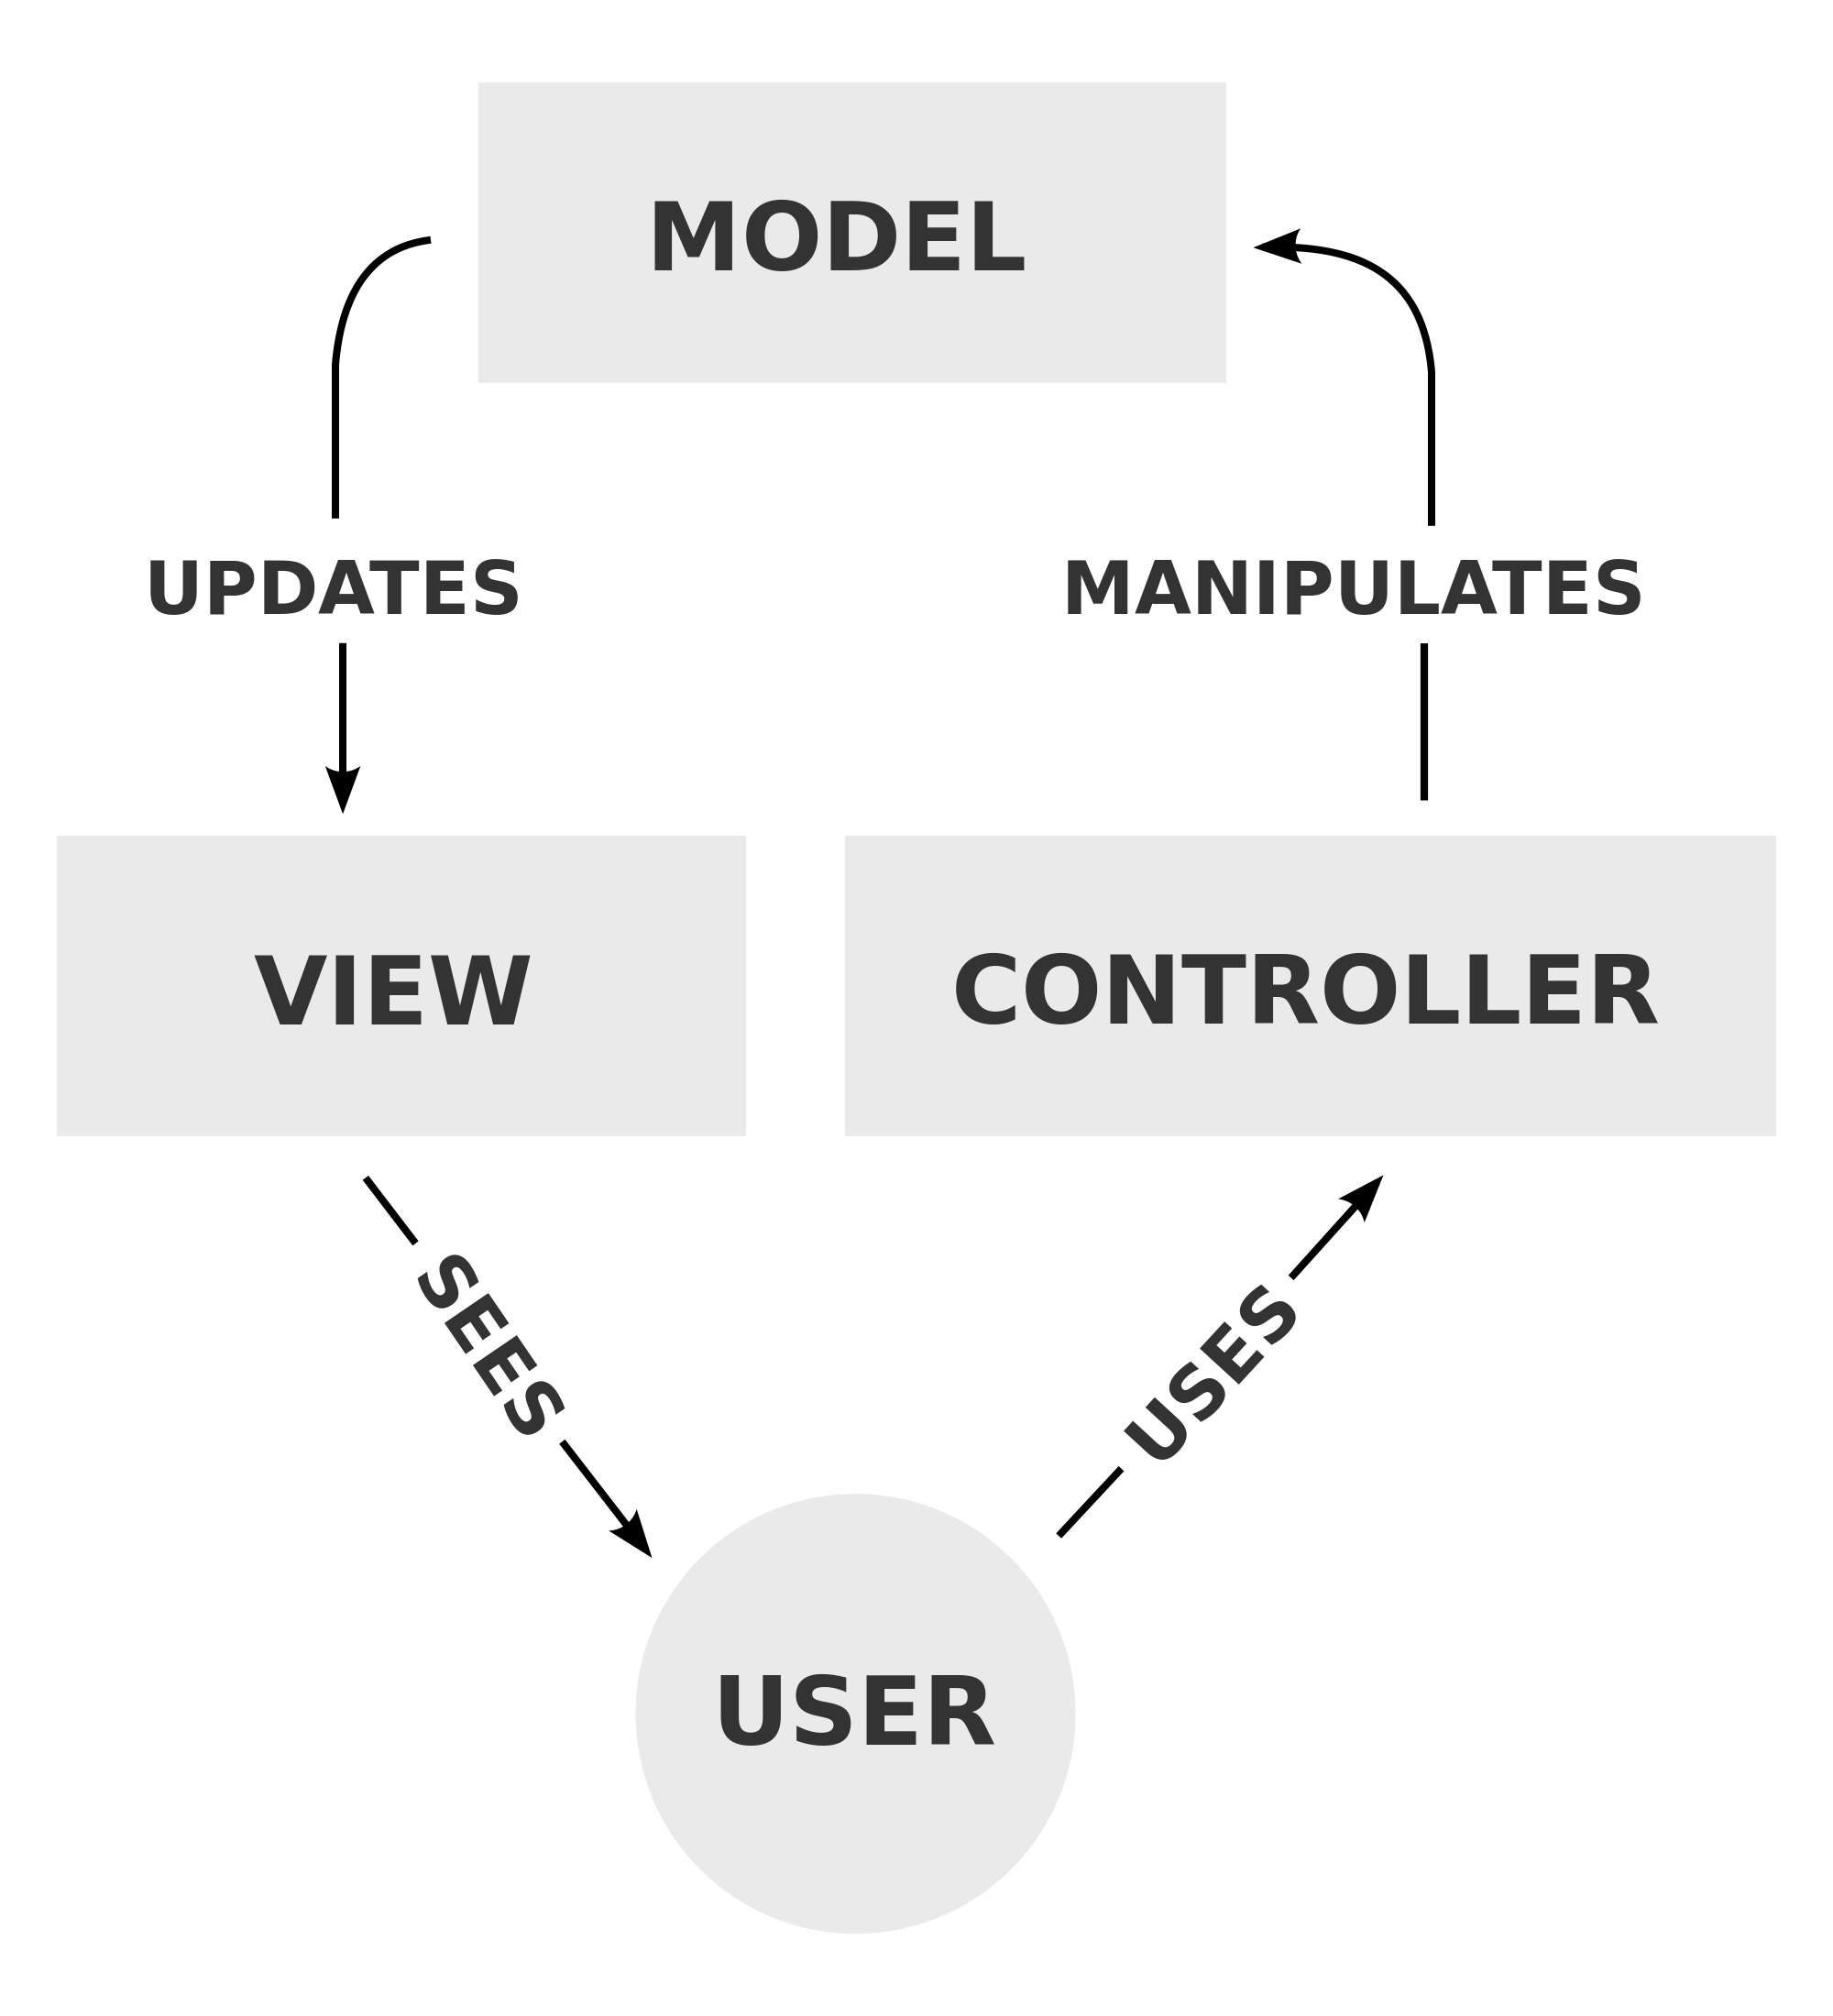
\includegraphics[width=0.7\textwidth]{mvcpattern.png}
	    \caption{Αρχιτεκτονική MVC.}
	    \label{fig:mvc_pattern}
	\end{figure}
		
		
		Η  χρήση της αρχιτεκτονικής MVC κατά την δημιουργία μίας εφαρμογής μας προσφέρει τα εξής βασικά πλεονεκτήματα:
		\begin{itemize}
		\item Διαχωρισμός των προβλημάτων (Separation of Concerns). Ουσιαστικά δημιουργείται μία εφαρμογή η οποία έχει τρία επίπεδα(models, views, controllers) και το κάθε επίπεδο επιτελεί ξεχωριστό έργο και ταυτόχρονα συνεργάζεται με τα άλλα επίπεδα. Στην σωστή υλοποίηση πρέπει τα τρία επίπεδα να είναι πλήρως καθορισμένα και να μην συμπλέκονται. Ο διαχωρισμός αυτός, επιτρέπει την επαναχρησιμοποίηση της επιχειρηματικής λογικής σε διάφορες εφαρμογές και την ανάπτυξη πολλαπλών user interfaces χωρίς να προβληματιζόμαστε από τον κώδικα που διαχειρίζεται την βάση.
		\item \textbf{Επεκτασιμότητα (Scaleability)}. Είναι η δυνατότητα που διαθέτει μία εφαρμογή , να μπορούμε μελλοντικά να προσθέσουμε λειτουργίες σε αυτή ή να αλλάξουμε κάποιες από τις ήδη υπάρχουσες λειτουργίες με σκοπό να επιτύχουμε διαφορετικά αποτελέσματα. 
		\item \textbf{Ελεγξιμότητα (Testability)}. Οι MVC εφαρμογές έχουν τη δυνατότητα να είναι πιο εύκολα ελέγξιμες και με τον τρόπο αυτόν συντηρούνται πιο εύκολα.  Εφόσον τα συστατικά της αρχιτεκτονικής είναι διακριτά, είναι πιο εύκολο να γράφουμε κώδικα που να τεστάρει ξεχωριστά το κάθε κομμάτι, γρήγορα και αποτελεσματικά.
		\item \textbf{Παράλληλη ανάπτυξη από διαφορετικές ομάδες}. Οι προγραμματιστές επιχειρηματικής λογικής  μπορούν να δημιουργούν τις κλάσεις, ενώ οι προγραμματιστές του user interface μπορούν να σχεδιάζουν ταυτόχρονα τις οθόνες. Επίσης μπορούν να γίνονται ενημερώσεις και αλλαγές στο user interface χωρίς να επιβραδύνεται η διαδικασία του business logic.
		\end{itemize}
		
	\subsubsection{MVP αρχιτεκτονικό πρότυπο}\label{sssect:MVP_architecture}
	Το αρχιτεκτονικό πρότυπο Model View Presenter (MVP) αποτελεί ένα παράγωγο αρχιτεκτονικό πρότυπο του MVC \cite{mvpPotel}, το οποίο είναι πολύ δημοφιλές στην ανάπτυξη εφαρμογών για το λειτουργικό σύστημα Android. Στην θεωρία τουλάχιστον, οι εφαρμογές Android είναι στημένες με τη λογική του MVC \cite{androidArchAnalysis}, όπως περιγράφηκε στην ενότητα \ref{sssection:mvc}, με το Activity ή το Fragment να αποτελεί τον controller και τα xml layouts τα views. Στην πράξη όμως καταλήγει η πλειονότητα του view logic να βρίσκεται στο Activity το οποίο το μετατρέπει σε δομή model-view όπως φαίνεται στο σχήμα \ref{fig:model_view}, κάτι το οποίο σε καμία περίπτωση δεν είναι το επιθυμητό. Στόχος λοιπόν του MVP είναι να λύσει ακριβώς αυτό το πρόβλημα και να πετύχει πλήρη διαχωρισμό μεταξύ του view και του view logic όπως βλέπουμε στο σχήμα \ref{fig:mvp_pattern}.
		
	 \begin{figure}[h]
	    \centering
	    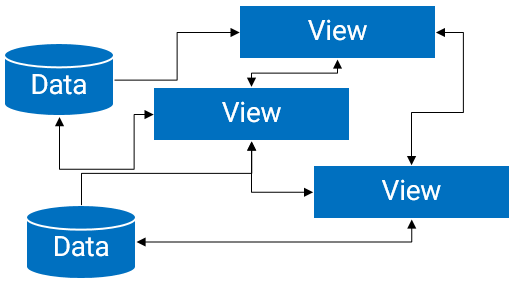
\includegraphics[width=0.7\textwidth]{model_view.png}
	    \caption{Android Model-View αρχιτεκτονικό πρότυπο.}
	    \label{fig:model_view}
	\end{figure}
	
	\begin{figure}[h]
	    \centering
	    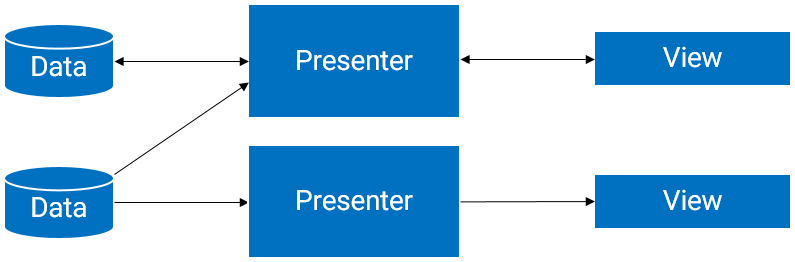
\includegraphics[width=0.7\textwidth]{mvp_pattern.png}
	    \caption{Android MVP αρχιτεκτονικό πρότυπο.}
	    \label{fig:mvp_pattern}
	\end{figure}
	
	Πλεονεκτήματα και λόγοι χρήσης του αρχιτεκτονικού προτύπου Model View Presenter\cite{androidHacks}:
	\begin{itemize}
		\item \textbf{Επεκτασιμότητα} η οποία επιτυγχάνεται μέσω του πλήρη διαχωρισμού μεταξύ της εμφάνισης (view) και της λογικής της εμφάνισης (view logic). 
		\item \textbf{Ευκολία Testing} του κάθε στρώματος (layer) της εφαρμογής αφού έχουμε πετύχει σαφή διαχωρισμό μεταξύ τους. Εν γένει η χρήση του μοτίβου MVP προάγει το test driven development της εφαρμογής με όλα τα πλεονεκτήματα που συνεπάγεται η εν λόγω τεχνική ανάπτυξης.
	\end{itemize}
	
	Το αρχιτεκτονικό πρότυπο MVP όπως δηλώνει και το όνομα του αποτελείται από τα παρακάτω τρία στοιχεία α) Model β) View γ) Presenter :
	\begin{itemize}
		\item \textbf{Model: } Το model στο αρχιτεκτονικό πρότυπο MVP επιτελεί της ίδιες λειτουργίες με αυτές στο MVC όπως περιγράφηκαν παραπάνω στην ενότητα \ref{sssection:mvc}.
		\item \textbf{View: } Το view υλοποιείται συνήθως μέσω κάποιου Activity ή Fragment (εξαρτάται από τη συγκεκριμένη αρχιτεκτονική της εφαρμογής), και περιέχει αναφορά στον presenter ο οποίος το χειρίζεται. H εν λόγω αναφορά πραγματοποιείται με χρήση του σχεδιαστικού μοτίβου dependency injection και ιδανικά με χρήση του Dagger. Κάθε φορά που ο χρήστης αλληλεπιδρά με κάποια λειτουργία (π.χ κουμπί) του view, καλείται η αντίστοιχη συνάρτηση του presenter ο οποίος επικοινωνεί με το model και λέει εν τέλει στο view τι θα εμφανίσει.
		\item \textbf{Presenter: } Ο Presenter είναι λειτουργεί ως το ενδιάμεσο στάδιο - ενορχηστρωτής μεταξύ του view και του model. Είναι υπεύθυνος για την απόκτηση των δεδομένων από το model και την παρουσίαση τους στο view, αλλά σε αντίθεση με την κλασσική αρχιτεκτονική MVC είναι υπεύθυνος για τις αλλαγές που γίνονται στο view όταν ο χρήστης αλληλεπιδρά μαζί του.
	\end{itemize}
	
	Για να αποσαφηνιστεί πλήρως η λειτουργία του και να γίνει πιο εύκολα κατανοητό στο σχήμα \ref{fig:mvp_workflow} βλέπουμε ένα χαρακτηριστικό παράδειγμα.
	
	\begin{figure}[h]
	    \centering
	    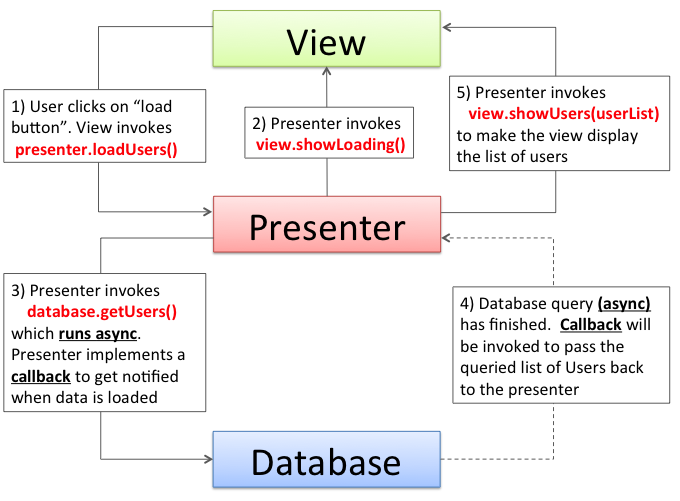
\includegraphics[width=0.7\textwidth]{mvp_workflow.png}
	    \caption{Παράδειγμα MVP σε Android.}
	    \label{fig:mvp_workflow}
	\end{figure}

	\subsection{Frameworks}
	
		Το framework, στον προγραμματισμό ηλεκτρονικών υπολογιστών, είναι μια αφηρημένη έννοια με την οποία κοινός κώδικας ο οποίος παρέχει γενικές λειτουργίες, μπορεί να επανεγγραφεί επιλεκτικά ή να εξειδικευτεί μέσω του κώδικα κάποιου χρήστη ώστε να χρησιμοποιηθεί για συγκεκριμένες λειτουργίες. Τα frameworks είναι μια ειδική περίπτωση βιβλιοθηκών λογισμικού που εμπεριέχουν επαναχρησιμοποιήσιμα κομμάτια κώδικα σε μια καλά καθορισμένη διεπαφή προγραμματισμού εφαρμογών (API), που όμως περιέχουν κάποια βασικά χαρακτηριστικά γνωρίσματα που τα διαφοροποιούν από τις κανονικές βιβλιοθήκες. Κάποια από τα γνωρίσματα αυτά είναι: αντιστροφή του ελέγχου (η ροή του προγράμματος υπαγορεύεται από το framework και όχι από αυτόν που το χρησιμοποιεί), προκαθορισμένη συμπεριφορά, επεκτασιμότητα (μπορεί να επεκταθεί από το χρήστη συνήθως με επανεγγραφή  ή εξειδίκευση του κώδικα ώστε να εκτελούνται συγκεκριμένες λειτουργίες. \cite{Framework}

	
		\subsubsection{Express Framework}


		Το Express είναι ένα δρομολόγησης και middleware framework, το οποίο έχει ελάχιστη λειτουργικότητα από μόνο του. Μια Express εφαρμογή ουσιαστικά αποτελεί μία σειρά από middleware κλήσεις. Ο δημιουργός του Express framework, TJ Holowaychuck, το έχει περιγράψει ως "Sinatra Inspired Server",  που σημαίνει ότι είναι σχετικά ελάχιστο, αλλά παρέχει πολλά επιπλέον χαρακτηριστικά, τα οποία είναι διαθέσιμα ως πρόσθετα. 
		
Το middleware είναι μια συνάρτηση με πρόσβαση στο αντικείμενο της αίτησης (req), το αντικείμενο απάντηση (res), και το επόμενο middleware στον κύκλο αίτησης-απάντησης της εφαρμογής, που συνήθως συμβολίζεται με μια μεταβλητή με το όνομα next.

Το middleware μπορεί να:

\begin{itemize}

\item Εκτελέσει οποιοδήποτε κώδικα.
\item Να κάνει αλλαγές στην αντικείμενα αίτησης και απάντησης(request and response objects).
\item Να τερματίσει τον κύκλο αίτησης-απάντησης.
\item Να καλέσει το επόμενο middleware της στοίβας.
\item Εάν το τρέχον middleware δεν τελειώσει τον κύκλο αίτησης-απάντησης, θα πρέπει να κληθεί το επόμενο, next(), για να περάσει ο έλεγχος στο επόμενο middleware, διαφορετικά η αίτηση θα μείνει ξεκρέμαστη.

\end{itemize}


Μία εφαρμογή Express μπορεί να χρησιμοποιήσει τα ακόλουθα είδη middleware: middleware επιπέδου εφαρμογής (application-level middleware),middleware επιπέδου δρομολόγησης, middleware χειρισμού σφαλμάτων(error-handling middleware), ενσωματωμένο middleware (built-in middleware), middleware τρίτων κατασκευαστών middleware (third-party middleware). 


		\subsubsection{Angular}
		
		Το AngularJS είναι ένα από τα πιο δημοφιλή ανοιχτού κώδικα JavaScript framework που χρησιμοποιείται για την κατασκευή και τη δομή σύγχρονων διαδικτυακών εφαρμογών, κυρίως εφαρμογών μίας σελίδας. Αναπτύχθηκε από τη Google και από μία κοινότητα προγραμματιστών για την αντιμετώπιση των πολλών προκλήσεων που ανέκυψαν κατά την ανάπτυξη των εφαρμογών μίας σελίδας. Στόχος του είναι να απλοποιήσει τόσο την ανάπτυξη όσο και το testing αυτών των εφαρμογών, παρέχοντας ένα framework για client-side model-View-Controller (MVC) και το model-view-viewmodel (MVVM) αρχιτεκτονικές, μαζί με τα συστατικά που χρησιμοποιούνται συνήθως στις εφαρμογές Διαδικτύου.
	   \\*
			    \textbf{Αρχιτεκτονική}
	 \\*
		Κατά την εκκίνηση της εφαρμογής, το πρόγραμμα περιήγησης φορτώνει το HTML αρχείο και το κάνει ``'parse' στο DOM αρχείο, και μαζί με αυτό στο AngularJs script. Μόλις το DOM αρχείο έχει φορτωθεί, το AngularJS αναζητά την εντολή ng-app η οποία ορίζει τα όρια της εφαρμογής. Εάν ορίζεται κάποιο module μέσα στην οδηγία, τότε χρησιμοποιείται για να ρυθμιστεί το \$injector, που δημιουργεί τo \$compile service καθώς και το \$ rootScope. Τότε μεταγλωττίζεται το DOM και συνδέεται στο \$ rootScope μετά από το οποίο εκτελούνται οι υπόλοιπες εντολές (αν υπάρχουν). Στο σχήμα \ref{fig:angularjs} φαίνεται ο κύκλος εκκίνησης του AngularJS.
		
	  \begin{figure}[h]
	    \centering
	    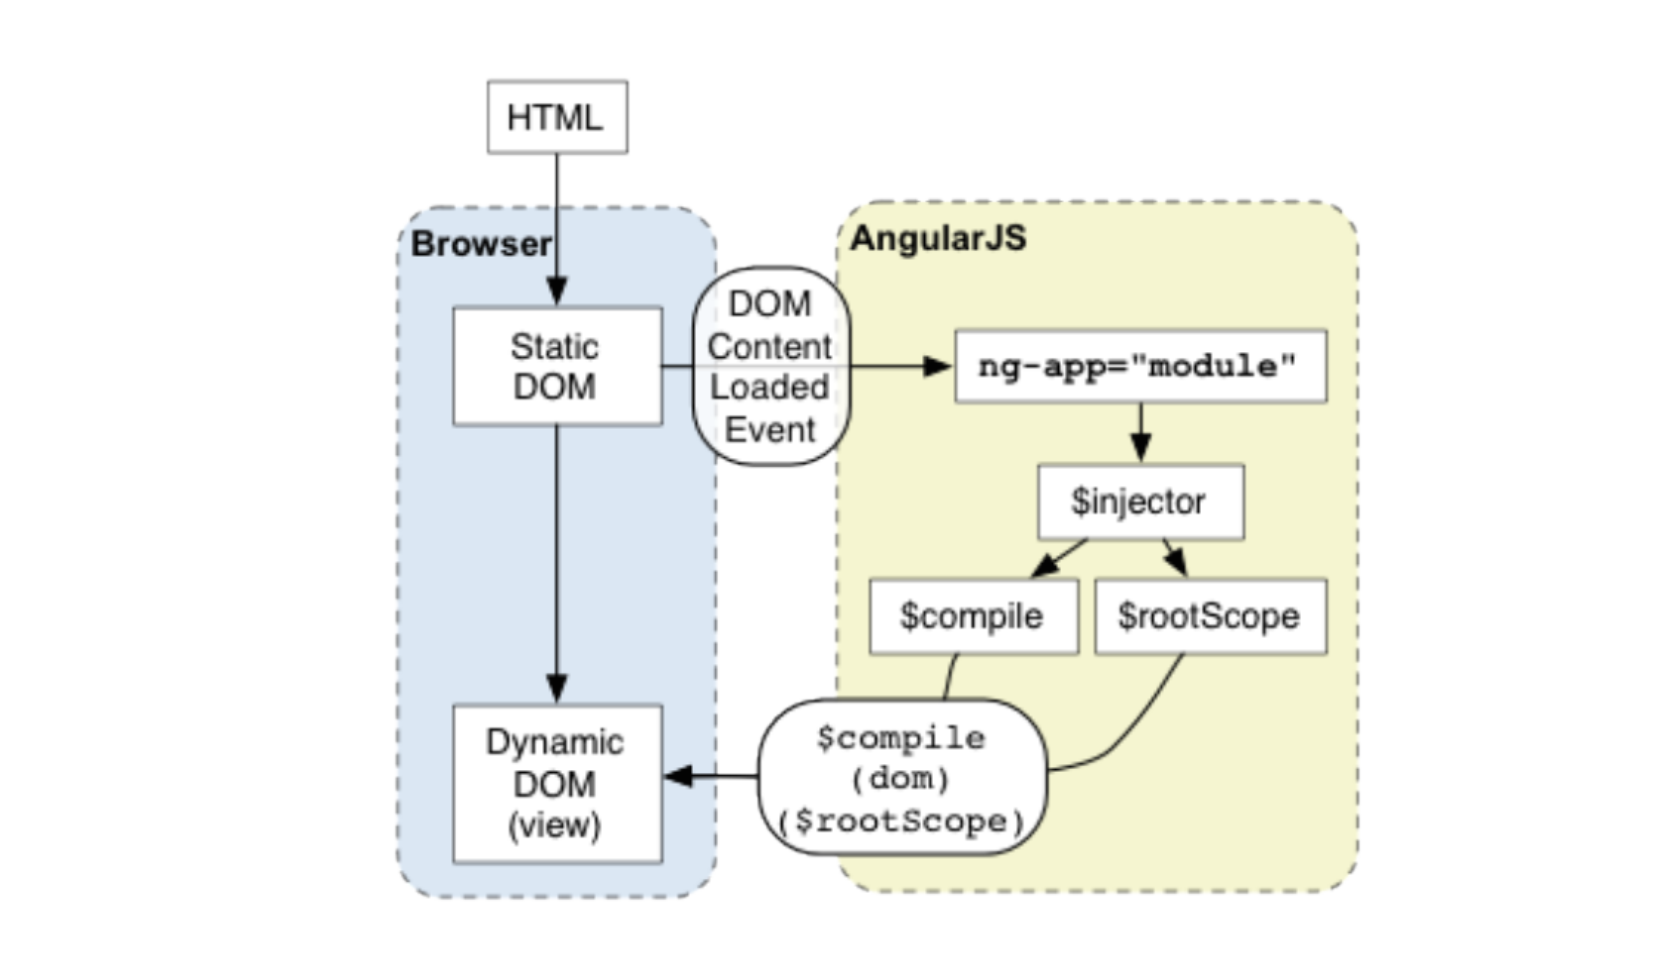
\includegraphics[width=0.7\textwidth]{angularjs.png}
	    \caption{AngularJS κύκλος εκκίνησης.}
	    \label{fig:angularjs}
	\end{figure}

	Κάποια από τα βασικά χαρακτηριστικά του AngularJS είναι:
	\begin{itemize}
	\item Two Way Data-binding. Αυτό πρακτικά σημαίνει ότι όταν αλλάζει το model αλλάζει και το view, και όταν αλλάζει το  view αλλάζει και το model. Το Two Way Data-binding εξηγείται καλύτερα με ένα παράδειγμα: 
	
	
	\lstinputlisting[language=Html]{two_way_data_binding.html}

	Αν ο χρήστης αλλάζει κάποια τιμή του model μέσω της εισόδου στο view, τότε το AngularJs αποθηκεύει την τιμή
αυτή σε μια μεταβλητή. Το στοιχείο h1 στην συνέχεια ενημερώνεται αυτόματα ώστε να αντικατοπτρίζονται οι αλλαγές στην τιμή της μεταβλητής του model. Το view ενημερώνεται ακόμα και αν η μεταβλητή αλλάξει χειροκίνητα με χρήση JavaScript.\cite{angular}

	\item  HTML Templates. Ενώ άλλα JavaScript frameworks χρησιμοποιούν ένα template system που βασίζεται στην HTML με ειδική σήμανση το οποίο μπορεί να είναι δυσκολεύει τους προγραμματιστές, το AngularJS δεν στηρίζεται σε εξωτερικές template engines αλλά χρησιμοποιεί ένα templating σύστημα, που είναι χτισμένη πάνω στην HTML με έξυπνη χρήση των ng- χαρακτηριστικών. Το πρόγραμμα περιήγησης διαβάζει την HTML και ``ψάχνει"  ng - directives τα οποία, όταν εκτελεστούν, δεσμεύουν το view στο model.

    \item Dependency Injection. Το dependency injection ενθαρρύνεται πολύ από το AngularJS και είναι ένα από τα συστατικά του, που βελτιώνει σε μεγάλο βαθμό το testability του. Το dependency injection είναι ένα design pattern λογισμικού στο οποίο σε ένα αντικείμενο ορίζονται οι εξαρτήσεις του και δεν τις δημιουργεί μόνο του. Πρόκειται ουσιαστικά για την αφαίρεση των hard-coded εξαρτήσεων, κάνοντας δυνατό να αλλάξουν οι εξαρτήσεις όποτε χρειαστεί.
      Ένα παράδειγμα είναι όταν υπάρχει μία συνάρτηση η οποία παίρνει μία παράμετρο, όπως:
    	
	\lstinputlisting[language=JavaScript]{angular_dependency_injection.js}

Το παραπάνω παράδειγμα είναι εύκολο να το τεστάρουμε, επειδή το στοιχείο που εισάγεται στην συνάρτηση μπορεί να είναι είτε ένα πραγματικό αντικείμενο ή ένα αντικείμενο για τους σκοπούς των τεστ. Ο διαχωρισμός σε μικρότερα πιο εύκολα ελέγξιμα συστατικά μπορεί να βοηθήσει πολύ στην ανίχνευση των σφαλμάτων.

    \item Deep Linking. Σε μια εφαρμογή μίας σελίδας είναι σημαντικό να διατηρείται η κατάσταση της εφαρμογής στο url, έτσι ώστε οι χρήστες είναι σε θέση να βάλουν κάποιο σελιδοδείκτη ή να μοιραστούν κάποιον σύνδεσμο σε διάφορες καταστάσεις της εφαρμογής.Το AngularJS χρησιμοποιεί το HTML5 history API  μαζί με ένα (\#!) εφεδρικό για παλαιότερα προγράμματα περιήγησης. Η λειτουργία αυτή είναι εξαιρετικά ισχυρή στη σύγχρονη εποχή των κοινωνικών δικτύων και του sharing.

	\item Directives. Τα directives είναι κάτι μοναδικό στο AngularJS και επιτρέπουν την επέκταση της λειτουργικότητας της HTML. Ενώ το AngularJS έχει μια συλλογή από προκαθορισμένα directives, μπορεί να επεκταθεί με συγκεκριμένες λειτουργικότητες σε σημείο που να επιτρέπει στον χρήστη να δημιουργήσει το δικό του DSL (Domain specific language). Επίσης επιτρέπει να δημιουργηθούν προσαρμοσμένα στοιχεία DOM, καθώς και χαρακτηριστικά και κλάσεις στα οποία μπορούν να προστεθούν λειτουργικότητες. Το επόμενο παράδειγμα από το επίσημο documentation του AngularJS δείχνει ότι για παράδειγμα γίνεται να επιτραπούν data-bindings για ένα html στοιχείο, αν υπάρχει ένα συγκεκριμένο χαρακτηριστικό. \cite{angular-directives}
\\*
\textbf{HTML:}

	\lstinputlisting[language=Html]{angular_directives.html}
 
\textbf{JavaScript:}

	\lstinputlisting[language=JavaScript]{angular_directives.js}


	\item \$http service. Το AngularJS είναι εξαιρετικά ευέλικτο στον τρόπο που επικοινωνεί με τα διαφορετικά backends. Αντί να βασίζεται αποκλειστικά στο REST, επικοινωνεί ελεύθερα μέσω των XMLHttpRequests του προγράμματος περιήγησης ή μέσω του JSONP. Παρόλο που το \$ http service προσθέτει http headers ως προεπιλογή στα αιτήματα του,  είναι εύκολα διαμορφώσιμα μέσω του \$httpProvider.defaults.headers.
	\end{itemize}




		\subsubsection{Bootstrap}
	Το bootstrap είναι ένα πάρα πολύ δυνατό front-end framework για την ταχύτερη και ευκολότερη ανάπτυξη ιστοσελίδων. Είναι ουσιαστικά μία συλλογή εργαλείων ανοιχτού κώδικα και περιλαμβάνει HTML και CSS πρότυπα σχεδιασμού για κοινά στοιχεία διεπαφής χρήστη, όπως τυπογραφίας, φόρμες, κουμπιά, πίνακες, dropdowns, alerts, μπάρες, και πολλά άλλα, καθώς και προαιρετικές επεκτάσεις JavaScript. Το bootstrap είναι συμβατό με όλες τις τελευταίες εκδόσεις των προγραμμάτων πλοήγησης και υποστηρίζει "responsive web design". Αυτό σημαίνει πως η διάταξη των ιστοσελίδων προσαρμόζεται δυναμικά, λαμβάνοντας υπόψιν τα χαρακτηριστικά της συσκευής που το χρησιμοποιεί (σταθερός υπολογιστής, κινητό, τάμπλετ κ.τ.λ.). 
	
	Το bootstrap είναι modular και αποτελείται από μικρότερα LESS stylesheets τα οποία υλοποιούν τα διάφορα στοιχεία του πακέτου εργαλείων. Ένα stylesheet, με όνομα bootstrap.less περιλαμβάνει τα επιμέρους stylesheets. Οι προγραμματιστές μπορούν να προσαρμόσουν και οι ίδιοι το bootstrap, καθώς τους δίνεται η δυνατότητα να επιλέξουν τα στοιχεία που θέλουν να χρησιμοποιήσουν. Αναπροσαρμογές γίνονται σε περιορισμένο όμως βαθμό, μέσω ενός κεντρικού stylesheet. Πιο ουσιαστικές αλλαγές πραγματοποιούνται με LESS δηλώσεις. Η χρήση των LESS stylesheets επιτρέπει τη χρήση μεταβλητών, συναρτήσεων καθώς και mixins. Επιπλέον, ο σχεδιαστής μπορεί να επιλέγει σε μια φόρμα τα επιθυμητά στοιχεία και να τα προσαρμόζει, σε τιμές διαφόρων εναλλακτικών λύσεων για τις ανάγκες του. Στη συνέχεια δημιουργείται ένα πακέτο που περιλαμβάνει ήδη το προ-χτισμένο CSS stylesheet.
	
	Το bootstrap παρέχει ένα σύνολο από stylesheets που παρέχουν βασικούς ορισμούς στυλ για όλα τα βασικά HTML στοιχεία. Αυτά παρέχουν ενιαία, σύγχρονη εμφάνιση για πίνακες, μορφοποίηση κειμένου, καθώς και για τα στοιχεία μιας φόρμας. Επιπλέον των HTML στοιχείων, το bootstrap περιέχει και άλλα στοιχεία περιβάλλοντος τα οποία χρησιμοποιούνται συχνά. Αυτά περιλαμβάνουν κουμπιά με προηγμένα χαρακτηριστικά ( π.χ. ομαδοποίηση κουμπιών ή drop-down επιλογή, οριζόντιες και κάθετες καρτέλες, σελιδοποίηση, κ.λ.π. ), ετικέτες, προηγμένες τυπογραφικές δυνατότητες, εικονίδια, προειδοποιητικά μηνύματα και μια γραμμή προόδου. Τέλος, το bootstrap περιέχει πολλά συστατικά JavaScript σε μια μορφή jQuery plugin, τα οποία παρέχουν πρόσθετα στοιχεία διεπαφής χρήστη όπως παράθυρα διαλόγου, επεξηγήσεις, και καρουσέλ. Μπορούν επίσης να επεκτείνουν τη λειτουργικότητα ορισμένων υφιστάμενων στοιχείων της διασύνδεσης, όπως για παράδειγμα μια αυτόματη πλήρη λειτουργία για πεδία εισαγωγής\cite{bootstrap}. 
	Τα πιο σημαντικά πλεονεκτήματα που προκύπτουν από την χρήση του bootstrap είναι:
	\begin{itemize}
	\item \textbf{Ταχύτητα ανάπτυξης: } Αδιαμφισβήτητα, ένα από τα σημαντικότερα πλεονεκτήματα της χρήσης του bootstrap είναι η ταχύτητα της ανάπτυξης. Το bootstrap παρέχει τη δυνατότητα χρήσης έτοιμων μπλοκ κώδικα, έτσι ώστε να γίνεται η αρχή του front-end από εκεί και να μην χρειάζεται να γραφτεί κώδικας από το μηδέν ("from scratch"). Το άνωθεν σε συνδυασμό με τη συμβατότητα σε όλα τα προγράμματα περιήγησης που προσφέρει καθώς και τις λειτουργίες του CSS-LESS, εξοικονομεί πολύτιμο χρόνο στους προγραμματιστές.
	\item \textbf{Ανταποκρισημότητα: } Λόγω του διαρκώς αυξανόμενου αριθμού των κινητών συσκευών υπάρχει η ανάγκη να έχουμε διαδραστικές ιστοσελίδες.Το bootstrap διευκολύνει πάρα πολύ την δημιουργία οθονών για κινητά χάρη στη ρευστή διάταξη πλέγματος που έχει, η οποία προσαρμόζεται δυναμικά στην κατάλληλη ανάλυση οθόνης και δεν χρειάζεται να προβούμε σε επιπλέον ενέργειες για να πετύχουμε την σωστή αποκρισιμότητα.
	\item \textbf{Συνοχή: } Το bootstrap βασίζεται σε αυτή την αρχή καθώς αρχικά αναπτύχθηκε από μερικούς υπαλλήλους του Twitter ως ένα framework για να υπάρχει συνέπεια μεταξύ των εσωτερικών εργαλείων που χρησιμοποιούνταν. Το bootstrap ουσιαστικά χτίστηκε ώστε να "ταιριάζει" τους σχεδιαστές με τους προγραμματιστές και να διασφαλίζει τη συνέπεια, ανεξάρτητα του ποιος εργάζεται στο έργο ή σε ποια πλατφόρμα θα τρέξει.
	\item \textbf{Προσαρμοστικότητα: } Το bootstrap, μπορεί να προσαρμοστεί σύμφωνα με τις προδιαγραφές του κάθε έργου. Οι προγραμματιστές έχουν τη δυνατότητα να επιλέξουν τα χαρακτηριστικά που χρειάζονται και να πετάξουν τα υπόλοιπα.
	\end{itemize}

		
	\subsection{Jade Template Engine}
	

	Μια μηχανή πρότυπο είναι μια βιβλιοθήκη ή ένα framework που χρησιμοποιεί ορισμένους κανόνες ή μία συγκεκριμένη γλώσσα για να ερμηνεύσει τα δεδομένα και να παρουσιάσει τα views. Στην περίπτωση των διαδικτυακών εφαρμογών, τα views είναι σελίδες HTML (ή τμήματα αυτών), αλλά γενικότερα μπορεί να είναι JSON ή XML αρχεία, ή graphic user interfaces. Με βάση το μοντέλο Model-View-Controller (MVC), τα πρότυπα ανήκουν στα views.

		Υπάρχουν πολλοί λόγοι που οδηγούν στη χρήση μιας μηχανή προτύπων αντί για την συγγραφή του front-end κώδικα σε μια συγκεκριμένη γλώσσα. Το μεγάλο πλεονέκτημα αυτής της προσέγγισης, είναι ότι παρουσιάζει HTML στην πλευρά του εξυπηρετητή (server), την οποία στέλνει στον πελάτη (client) και στη συνέχεια όταν ο πελάτης αλληλεπιδράσει με τη σελίδα και η HTML αλλάξει χρησιμοποιώντας τα ίδια bits του πρότυπου και ίσως ακόμη και κάποια κοινή λογική. Άλλοι πολύ σημαντικοί λόγοι αποτελούν η συνέπεια του κώδικα και η οργάνωση.  Εάν υπάρχει καλός διαχωρισμός της σήμανσης (markup) από τη λογική γίνεται πιο εύκολος εντοπισμός σφαλμάτων του κώδικα, κοινή χρήση του κώδικα με συνεργάτες,καθώς και επιτυγχάνεται ταχύτερη ανάπτυξη μέσω της απόκτησης κοινών μεθόδων για την έξοδο της σήμανσης (markup). Οι μηχανές προτύπων που λειτουργούν, εξίσου καλά και από την πλευρά του εξυπηρετητή (server), όπως και από την πλευρά του πελάτη (client) αξιοποιούν το πλεονέκτημα ότι της ισομορφικής JavaScript, δηλαδή τη δυνατότητα που υπάρχει να τρέξει ο ίδιος κώδικας παντού.
	\cite{jade}

		Η μηχανή προτύπων Jade (Jade Template Engine)  είναι μία μηχανή υψηλής απόδοσης η οποία έχει επηρεαστεί σε μεγάλο βαθμό από το Haml και υλοποιήθηκε με χρήση Javascript για το Node. Η μηχανή Jade παράγει HTML, που χρησιμοποιείται στο πρόγραμμα περιήγησης στην πλευρά του εξυπηρετητή (server-side). Το πρόγραμμα περιήγησης(browser) εκτελεί μια αίτηση στον web-server, ο web-server εκτελεί την Jade, η οποία θα δημιουργήσει το HTML που θα πρέπει να σταλεί στον browser. Η μηχανή προτύπων Jade χρησιμοποιεί τα κενά και τις εσοχές ως μέρος της γλώσσας. Παράγει αυτόματα συμβατή σήμανση (markup) που βασίζεται σε μια ένθετη ιεραρχία με αναγνωριστικά ονόματα (tag names). Η μηχανή προτύπων Jade χρησιμοποιείται σε συνδυασμό με το framework ExpressJs σε πλατφόρμες ανάπτυξης NodeJs.

Τα πλεονεκτήματα της μηχανής προτύπων Jade είναι η ταχεία ανάπτυξη που εξασφαλίζεται, η συνοχή του παραγόμενου κώδικα και τα κοινά πρότυπα συμμόρφωσης. Επιπλέον, μας προσφέρει τη δυνατότητα να δημιουργήσουμε αμέτρητο αριθμό σελίδων δυναμικά με ένα ενιαίο πρότυπο. Τέλος, όταν προκύψει η ανάγκη να πραγματοποιηθεί μία αλλαγή, μπορεί  να αλλάξει ο κώδικας σε ένα μόνο σημείο και να εμφανισθεί σε όλες τις απαιτούμενες σελίδες. Παρακάτω	φαίνεται ένα παράδειγμα γραφής σε μηχανή προτύπων Jade.
	\lstinputlisting[language=JavaScript]{jade_example.jade}
	
	\subsection{Mockups}
	\subsection{Διασύνδεση με Social Networks}

\section{Mobile}
	\subsection{Mobile OS}
		Στην παρούσα ενότητα θα πραγματοποιήσουμε μια σύντομη σύγκριση μεταξύ των λειτουργικών συστημάτων iOS και Android. Περιορίζουμε την ανάλυση μόνο στα δύο προαναφερθείσα λειτουργικά γιατί αφενός έχουν τον μεγαλύτερο αριθμό ενεργών προγραμματιστών και αφετέρου τον μεγαλύτερο αριθμό χρηστών, κάτι που τα καθιστά τα πλέον διαδεδομένα λειτουργικά στην αγορά των έξυπνων κινητών. Στον πίνακα \ref{tab:android_vs_ios} βλέπουμε μια στοιχειώδη σύγκριση μεταξύ των δύο λειτουργικών \cite{smartphoneMarketShare}\cite{androidPublish}\cite{applePublish}\cite{androidSource}. Θα πρέπει να σημειωθεί ότι οι τιμές και τα στοιχεία που αναφέρονται στον πίνακα \ref{tab:android_vs_ios} είναι αυτά που ισχύουν κατά τη συγγραφή της παρούσας διπλωματικής (Οκτώβριος 2015).
		
	\begin{table}[H]
		\begin{center}
			\begin{tabular}{|l|c|c|}
			\hline
			\rowcolor{grayy}
			\textbf{Λειτουργικό} & \textbf{Android} & \textbf{iOS}
			\\ \hline
			Γλώσσα Προγραμματισμού & Java & Swift \\ \hline
			Περιβάλλον Ανάπτυξης & Android Studio & X-Code  \\ \hline
			Προσαρμοστικότητα & Μεγάλη & Ελάχιστη  \\ \hline
			Ανοιχτού Κώδικα & Ναι & Όχι  \\ \hline
			Μερίδιο Αγοράς & 82.8\% & 13.9\% \\ \hline
			Κόστος δημοσίευσης εφαρμογής & 25\$ εφάπαξ & 99\$/έτος  \\ \hline
			Έλεγχος Εφαρμογών & Όχι & Ναι \\ \hline
			\end{tabular}
			\caption{Σύγκριση βασικών στοιχείων Android \& iOS.}
			\label{tab:android_vs_ios}
		\end{center}
	\end{table}
	Σε αυτό το σημείο πρέπει να αναφέρουμε ότι το iOS Developer Toolset λειτουργεί μόνο στα πλαίσια του λειτουργικού Mac OS X. Επομένως, η ανάπτυξη μιας εγγενής iOS εφαρμογής προϋποθέτει την ύπαρξη ενός Apple υπολογιστή. Δεδομένου του μεγαλύτερου μεριδίου αγοράς που διαθέτει το Android καθώς και τις ευκολίες που παρέχει προς τους προγραμματιστές, το επιλέξαμε για την πιλοτική έκδοση της εφαρμογής μας.
	
	
	\subsection{Android}
	Στην παρούσα ενότητα θα αναφερθούμε στα βασικά δομικά στοιχεία και στην αρχιτεκτονική του λειτουργικού συστήματος Android.
	
		\subsubsection{Αρχιτεκτονική του Android}
		Το λειτουργικό σύστημα Android αποτελεί ουσιαστικά μια στοίβα πρωτοκόλλων για κινητά τερματικά που χωρίζεται σε πέντε κατηγορίες και τέσσερα επίπεδα όπως φαίνεται στο σχήμα \ref{fig:android_system_architecture}.
		
		\begin{figure}[h]
			\centering
			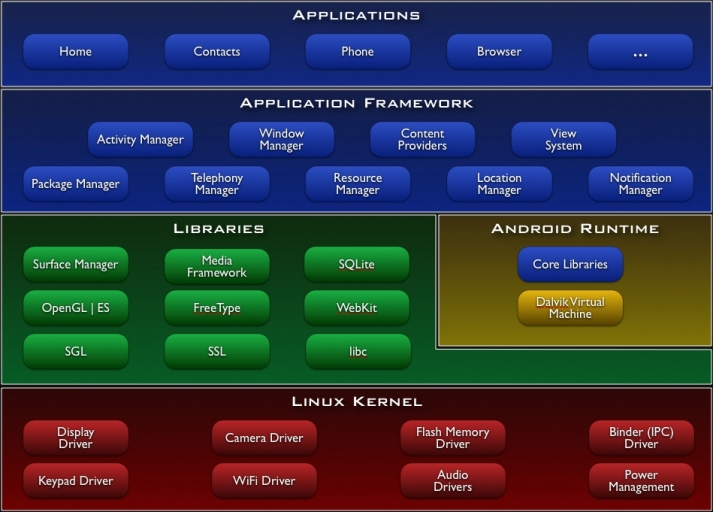
\includegraphics[width=0.9\textwidth]{android_system_architecture.jpg}
			\caption{Αρχιτεκτονική του λειτουργικού συστήματος Android}
			\label{fig:android_system_architecture}
		\end{figure}
		
		 Ξεκινώντας από το χαμηλότερο επίπεδο έχουμε \cite{collinsAndroid}\cite{annuzziAndroid}\cite{androidArchAnalysis}:
		 \begin{itemize}
		 	\item \textbf{Linux Kernel}: ο οποίος είναι ειδικά σχεδιασμένος για το λειτουργικό σύστημα Android και περιέχει τους οδηγούς για το υλικό (κάμερα, πληκτρολόγιο κ.τ.λ.). Επίσης ο πυρήνας είναι υπεύθυνος για τη διαχείριση της μνήμης και των διεργασιών, τις συνδέσεις δικτύου και κατ' επέκταση την διαχείριση των διεπαφών δικτύου που διαθέτει κάθε συσκευή. Επιπρόσθετα, χειρίζεται τους πόρους και την ενεργεία, κάτι το οποίο είναι πολύ σημαντικό δεδομένου της περιορισμένης παροχής ενέργειας των κινητών συσκευών. 
		 	\item \textbf{Libraries} Στο αμέσως επόμενο επίπεδο έχουμε τις βιβλιοθήκες του συστήματος, οι οποίες πολλές φορές αποκαλούνται και εγγενείς βιβλιοθήκες (Native Libraries). Οι εν λόγω βιβλιοθήκες έχουν αναπτυχθεί με χρήση των γλωσσών προγραμματισμού C και C++. Μερικές από τις πιο σημαντικές βιβλιοθήκες αυτού του επίπεδου είναι:
		 	\begin{itemize}
		 		\item WebKit, για την υποστήριξη των φυλλομετρητών
		 		\item Media Framework, για την αναπαραγωγή αρχείων ήχου και βίντεο
		 		\item Surface Manager, για τη δημιουργία παραθύρων και ανανέωση της οθόνης
		 		\item SQLite, για τη διαχείριση των βάσεων δεδομένων
		 		\item OpenGL, για την απόδοση γραφικών
		 		\item Text, για τον χειρισμό και την εμφάνιση κειμένου
		 	\end{itemize}
		 	Σε αυτό το επίπεδο βρίσκεται επίσης και το κομμάτι της εκτέλεσης του Android (Android Runtime), το οποίο υποστηρίζει τη διαδικασία εγγραφής και εκτέλεσης των εφαρμογών. Αποτελείται από δυο βασικές συνιστώσες:
		 	\begin{itemize}
		 		\item Βασικές βιβλιοθήκες για τη διεπαφή των εφαρμογών Java με το περιβάλλον της συσκευής στην οποία εκτελούνται. Πιο αναλυτικά, οι εν λόγω βιβλιοθήκες είναι δυναμικές, οι οποίες εισάγονται στην αρχή κάθε κλάσης.
		 		\item Την εικονική μηχανή Dalvik (Dalvik Virtual Machine) η οποία είναι υπεύθυνη για τη δημιουργία των εκτελέσιμων αρχείων των εφαρμογών. Συγκεκριμένα ο πηγαίος κώδικας Java μετατρέπεται σε μορφή ενδιάμεσου κώδικα (bytecode) και στην συνέχεια μεταφράζεται σε Dalvik bytecode που αποθηκεύεται σε αρχεία της μορφής .dex. Η διαδικασία της μετατροπής των αρχείων κλάσεων java σε μορφή .dex γίνεται από το εργαλείο dx, ενώ παράλληλα γίνεται και βελτιστοποίηση της πλεονάζουσας πληροφορίας με αποτέλεσμα τα αρχεία .dex να είναι μικρότερα σε μέγεθος από τα αντίστοιχα αρχεία κλάσεων. Τέλος, το αρχείο .dex μαζί με τους πόρους της εφαρμογής μετατρέπονται σε αρχείο της μορφή .apk (Android Package). Το .apk αρχείο είναι αυτό που χρησιμοποιείται από τον χρήστη για την εγκατάσταση της εφαρμογής στην συσκευή του. Όταν ο χρήστης εκτελέσει την εφαρμογή, τότε η εφαρμογή αυτή θα εκτελεστεί στην εικονική μηχανή Dalvik αντί της JVM, καθώς το περιβάλλον εκτέλεσης των κινητών συσκευών διαθέτει περιορισμένους πόρους.
		 	\end{itemize}
		 	\item \textbf{Application Framework} Στο τρίτο επίπεδο βρίσκεται το πλαίσιο λογισμικού των εφαρμογών, το οποίο ουσιαστικά είναι ένα σύνολο υπηρεσιών, οι οποίες δημιουργούν το περιβάλλον μέσα στο οποίο εκτελούνται οι εφαρμογές Android. Μερικές από τις πιο βασικές υπηρεσίες που περιλαμβάνονται στο επίπεδο του applicaiton framework είναι οι παρακάτω:
		 	\begin{itemize}
		 		\item Package Manager: Ο διαχειριστής πακέτων είναι το σύστημα μέσω του οποίου οι εφαρμογές μπορούν να βρουν πληροφορίες για τις υπόλοιπες εφαρμογές που είναι εγκατεστημένες στη συσκευή. Αποτελεί ουσιαστικά μια βάση δεδομένων όλων των εφαρμογών που είναι εγκατεστημένες στην συσκευή και επιτρέπει σε μια μια εφαρμογή να χρησιμοποιήσει μια άλλη και να μοιραστεί δεδομένα με αυτήν.
		 		\item Activity Manager: Ο διαχειριστής δραστηριοτήτων διαχειρίζεται τον κύκλο ζωής των εφαρμογών και τη στοίβα δραστηριοτήτων (activity stack).
		 		\item Content Providers: Οι πάροχοι περιεχομένου επιτρέπουν στις εφαρμογές να δημοσιεύουν και να μοιράζονται δεδομένα με άλλες εφαρμογές. Αποτελούν ουσιαστικά βάσεις δεδομένων οι οποίες δίνουν την δυνατότητα στις εφαρμογές να αποθηκεύσουν και να μοιραστούν δομημένες πληροφορίες. Παράδειγμα τέτοιων πληροφοριών αποτελούν οι επαφές της συσκευής.
		 		\item View System: Περιλαμβάνει γραφικά στοιχεία τα οποία χρησιμοποιούνται για τη δημιουργία της διεπαφής χρήστη. Παράδειγμα γραφικών στοιχείων που περιλαμβάνει είναι κουμπιά, κουτιά κειμένων, πλαίσια κ.τ.λ.
		 		\item Resource Manager: Ο διαχειριστής πόρων είναι υπεύθυνος για τη διαχείριση των πόρων που δεν αποτελούν κώδικα και κατ' επέκταση δεν μπορούν να μεταγλωττιστούν. Παράδειγμα τέτοιων στοιχείων αποτελούν τα γραφικά στοιχεία και οι συμβολοσειρές.
		 		\item Notification Manager: Ο διαχειριστής ειδοποιήσεων επιτρέπει στις εφαρμογές να εμφανίζουν ειδοποιήσεις προς το χρήστη. Οι ειδοποιήσεις αυτές εμφανίζονται στη μπάρα κατάστασης της συσκευής, η οποία βρίσκεται στο πάνω μέρος της οθόνης και είναι σχεδόν πάντα ορατή στον χρήστη.
		 		\item Telephony Manager: Ο διαχειριστής τηλεφωνίας παρέχει πληροφορίες στην εφαρμογή σχετικά με τις υπηρεσίες τηλεφώνου που είναι διαθέσιμες στην συσκευή.
		 		\item Location Manager: Ο διαχειριστής τοποθεσίας παρέχει στις εφαρμογές πρόσβαση σε πληροφορίες σχετικά με την τοποθεσία και την κίνηση της συσκευής.
		 	\end{itemize}
		 	\item \textbf{Applications} Στο τέταρτο και τελευταίο επίπεδο της αρχιτεκτονικής του λειτουργικού συστήματος Android βρίσκονται οι εφαρμογές. Σε αυτό το επίπεδο περιλαμβάνονται τόσο οι προεγκατεστημένες εφαρμογές όσο και οι εφαρμογές τρίτων.
		 \end{itemize}
		 
		\subsubsection{Δομικά στοιχεία του Android}
		Υπάρχουν τέσσερα βασικά δομικά στοιχεία στο λειτουργικό σύστημα Android (βλ. σχήμα \ref{fig:android_fundamental_components}). Κάθε δομικό στοιχείο επιτελεί ένα ξεχωριστό σκοπό και έχει ανεξάρτητο κύκλο ζωής. Κάθε δομικό στοιχείο αποτελεί ουσιαστικά ένα διαφορετικό σημείο, μέσω του οποίου το λειτουργικό σύστημα μπορεί να αποκτήσει πρόσβαση στην εφαρμογή. Στην συνέχεια θα κάνουμε μια συνοπτική παρουσίαση των βασικών αυτών δομικών στοιχειών, θεμελιώνοντας έτσι το θεωρητικό πλαίσιο για ανάπτυξη εφαρμογών Android \cite{androidComponentsKnoxville}\cite{androidFundamentalsOfficial}.
		
		\begin{figure}[h]
			\centering
			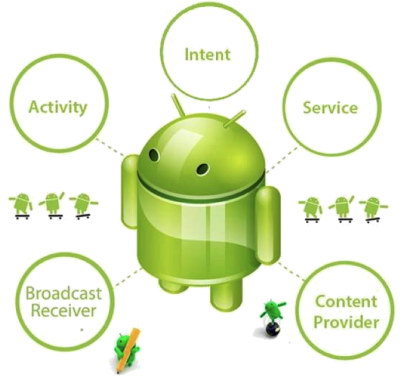
\includegraphics[width=0.6\textwidth]{android_fundamental_components.jpg}
			\caption{Δομικά στοιχεία του Android.}
			\label{fig:android_fundamental_components}
		\end{figure}
		
		\subsubsection{Activities}
		Η κλάση Activity αποτελεί τη βασικότερη κλάση μιας εφαρμογής Android. Κάθε κλάση Activity αποτελεί μια ξεχωριστή γραφική διεπιφάνεια (παράθυρο/οθόνη) μέσω της οποίας ο χρήστης αλληλεπιδρά με την εφαρμογή. Συνήθως το παράθυρο αυτό καλύπτει όλη την οθόνη της συσκευής αλλά υπάρχουν και κάποιες εξεζητημένες περιπτώσεις στις οποίες καλύπτει μόνο ένα μέρος της οθόνης.
		
		Κάθε εφαρμογή αποτελείται κατά κανόνα από πολλές Activities (οθόνες), οι οποίες είναι συνδεδεμένες μεταξύ τους, ενώ έχουν και την δυνατότητα ανταλλαγής πληροφοριών. Η οθόνη που παρουσιάζεται πρώτη στον χρήστη με το που πραγματοποιήσει εκκίνηση της εφαρμογής ονομάζεται `κύρια' (main), μέσω της οποίας μπορεί να πλοηγηθεί και στις υπόλοιπες οθόνες. Εν γένει κάθε activity έχει τη δυνατότητα να πραγματοποιήσει εκκίνηση μια άλλης activity. Το σύστημα κάθε φορά που γίνεται μετάβαση σε μια νέα activity εισχωρεί (push) την προηγούμενη σε μια στοίβα μορφής LIFO, που ονομάζεται back-stack, έτσι ώστε αν ο χρήστης πατήσει το κουμπί επιστροφής (back) να μπορεί με ένα pop στην στοίβα να επαναφέρει την αμέσως προηγούμενη activity. Δηλαδή αν ήμασταν αρχικά στην activity Α μέσω της οποία μεταβήκαμε στην Β, η activity Α βρίσκεται στην κορυφή της στοίβας οπότε με το πλήκτρο back οδηγούμαστε πάλι στην οθόνη που βρισκόμασταν προηγουμένως την Α. Σε αυτό το σημείο θα πρέπει να αναφερθεί ότι αν πατηθεί το κουμπί back όταν ο χρήστης βρίσκεται στην αρχική οθόνη και η στοίβα είναι άδεια, πραγματοποιείται έξοδος από την εφαρμογή.
		
		Για τη δημιουργία μιας οθόνης θα πρέπει να κάνουμε extend τη βασική κλάση Activity και να υλοποιήσουμε κάποιες απαραίτητες μεθόδους της. Συγκεκριμένα κάθε activity  πρέπει να υλοποιεί τη μέθοδο onCreate(), η οποία καλείται αυτόματα κατά την πρώτη εκκίνηση της activity όπως υπονοεί και το όνομα της. Θα πρέπει να τονιστεί ότι εκτελείται μόνο κατά την πρώτη δημιουργία του activity και όχι όταν επιστρέφουμε σε αυτό με χρήση του κουμπιού της επιστροφής. Μέσα στην εν λόγω μέθοδο γίνεται αρχικοποίηση των βασικών συστατικών που αποτελούν τη διεπαφή του χρήστη.
		
		Μια επίσης εκ των βασικών μεθόδων που πρέπει να υλοποιήσουμε αποτελεί το onPause(). Όπως υποδηλώνει και το όνομά της καλείται από το σύστημα όταν ο χρήστης πραγματοποιεί έξοδο από το συγκεκριμένο activity χωρίς όμως να το καταστρέφει, για παράδειγμα όταν κάνει μετάβαση σε άλλο activity της ίδιας εφαρμογής.
		
		Για να πραγματοποιήσουμε τον τερματισμό ενός activity αρκεί να εκτελεστεί η εντολή finish(), αν και συνήθως δεν χρειάζεται να τερματίζουμε εμείς τις acitivities αφού είναι κάτι που αποτελεί ουσιαστικά δικαιοδοσία του Dalvik. Για να γίνουν καλύτερα κατανοητά τα παραπάνω στο σχήμα \ref{fig:activity_lifecycle} βλέπουμε τον κύκλο ζωής των activities και τις αντίστοιχες μεθόδους.
		
		\begin{figure}[h]
			\centering
			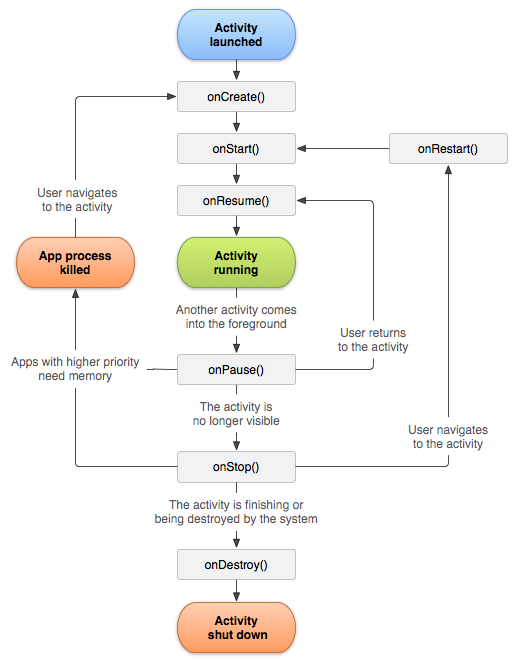
\includegraphics[width=0.5\textwidth]{activity_lifecycle.png}
			\caption{Ο κύκλος ζωής των activities.}
			\label{fig:activity_lifecycle}
		\end{figure}
		
		\subsubsection{Services}
		Οι υπηρεσίες αποτελούν τα στοιχεία μιας εφαρμογής, οι οποίες εκτελούν χρονοβόρες λειτουργίες στο παρασκήνιο (background) της εφαρμογής. Θεμελιώδη διαφορά μεταξύ μιας υπηρεσίας και ενός activity αποτελεί το γεγονός ότι η υπηρεσία δεν παρέχει κάποια διεπαφή προς τον χρήστη της εφαρμογής, δεδομένου ότι όπως προαναφέρθηκε δρουν παρασκηνιακά. Μια υπηρεσία έχει την δυνατότητα να συνεχίζει την εκτέλεση της στο παρασκήνιο ακόμα και στην περίπτωση όπου ο χρήστης έχει πραγματοποιήσει μετάβαση σε κάποια τελείως διαφορετική εφαρμογή. Ένα κλασσικό παράδειγμα υπηρεσίας αποτελεί η αναπαραγωγή μουσικής, η οποία συνεχίζει να εκτελείται στο παρασκήνιο ακόμα και όταν έχουμε κλείσει την εφαρμογή αναπαραγωγής μουσικής και εκτελούμε τελείως διαφορετικές εφαρμογές. Υπάρχουν κάποιες έτοιμες υπηρεσίες που μας παρέχει το λειτουργικό σύστημα όπως είναι ο Location Manager, αλλά μπορούμε να ορίσουμε και τις δικές μας υπηρεσίες. Μια υπηρεσία μπορεί ουσιαστικά να πάρει δυο διαφορετικές μορφές\cite{servicesAndroid}:
		\begin{itemize}
			\item Started: Μια υπηρεσία έχει εκκινηθεί όταν κάποιο συστατικό της εφαρμογής (π.χ ένα activity) έχει καλέσει τη μέθοδο startService(). Μόλις η υπηρεσία εκκινηθεί συνεχίζει να εκτελείται επ' αόριστον στο παρασκήνιο ακόμα και αν το activity που τηn κάλεσε έχει τερματιστεί. Συνήθως επιτελεί μία και μόνο εργασία χωρίς να επιστρέφει κάποιο αποτέλεσμα στο activity που την κάλεσε. Για παράδειγμα, μπορεί να κατεβάζει κάποιο αρχείο και όταν ολοκληρωθεί η μεταφόρτωση του θα τερματίσει η ίδια τον εαυτό της.
			\item Bound: Λέμε ότι μια υπηρεσία είναι ``δεμένη'' όταν κάποιο συστατικό της εφαρμογής (π.χ ένα activity) έχει καλέσει την μέθοδο bindService(). Μια `δεμένη' υπηρεσία παρέχει διεπαφή πελάτη - εξυπηρετητή (client - server) και επιτρέπει στα συστατικά της εφαρμογής που είναι συνδεδεμένα μαζί της να αλληλεπιδρούν με αυτήν, στέλνοντας αιτήματα και λαμβάνοντας τα αποτελέσματα ακόμα και αν βρίσκονται σε διαφορετικές διεργασίες χρησιμοποιώντας IPC (interprocess communication). Υπηρεσίες τέτοιου τύπου συνεχίζουν τη λειτουργία τους όσο τα συστατικά με τα οποία είναι συνδεδεμένα εξακολουθούν να τρέχουν. Η υπηρεσία τερματίζεται μόνο όταν τερματιστεί (ή αποσυνδεθεί) και το τελευταίο συστατικό που είναι συνδεδεμένο με αυτήν.
		\end{itemize}
		Όπως αναφέρθηκε προηγουμένως οι υπηρεσίες δεν παρέχουν κάποια διεπαφή προς τον χρήστη, οπότε δημιουργείται και το εύλογο ερώτημα για το πως θα ενημερώνεται ο χρήστης. Οι υπηρεσίες ειδοποιούν τους χρήστες για τα αποτελέσματα τους είτε με χρήση ειδοποίησης μορφής Toast είτε μέσω ειδοποίησης στο status bar.  Για να γίνουν καλύτερα κατανοητά οι έννοιες που αναλύθηκαν παραπάνω στο σχήμα \ref{fig:service_lifecycle} βλέπουμε τον κύκλο ζωής των υπηρεσιών.
		
		\begin{figure}[h]
			\centering
			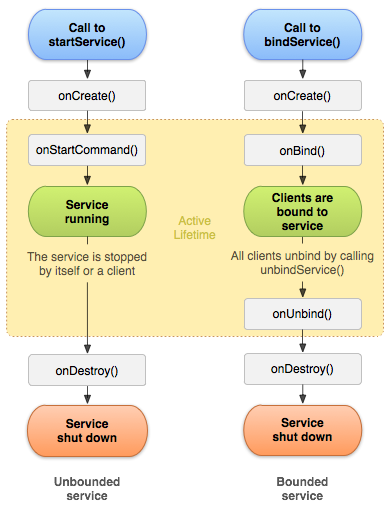
\includegraphics[width=0.5\textwidth]{service_lifecycle.png}
			\caption{Ο κύκλος ζωής των services}
			\label{fig:service_lifecycle}
		\end{figure}
		
		\subsubsection{Content Providers}
		Οι πάροχοι περιεχομένου διαχειρίζονται την πρόσβαση στους αποθηκευτικούς χώρους των δεδομένων. Ουσιαστικά, δημιουργείται η δυνατότητα αποθήκευσης και διαμοιρασμού δεδομένων στις εφαρμογές. Ένας πάροχος δεδομένων παρουσιάζει τα δεδομένα στις εφαρμογές σε μορφή πινάκων σαν τους πίνακες σε μια σχεσιακή βάση δεδομένων. Παράδειγμα ενός ενσωματωμένου παροχέα δεδομένων είναι το λεξικό χρήστη στο οποίο αποθηκεύονται οι λέξεις του χρήστη. Για αυτή τη χρήση υπάρχει και η ενσωματωμένη βάση δεδομένων SQLite, η οποία δίνει την δυνατότητα αποθηκεύσης και ανάγνωσης δεδομένων στους παρόχους περιεχομένου.\cite{androidContentProviders}
		\subsubsection{Broadcast Receivers}
		Οι δέκτες εκπεμπόμενων προθέσεων είναι υπεύθυνοι για τη λήψη και τη διαχείριση των γεγονότων που πραγματοποιούνται στην συσκευή. Συγκεκριμένα, ενημερώνονται από το λειτουργικό σύστημα όταν πραγματοποιείται κάποιο γεγονός και τότε ενεργοποιούνται. Χαρακτηριστικά παραδείγματα τέτοιων γεγονότων είναι όταν το κινητό μπαίνει σε κατάσταση αναμονής, όταν η στάθμη της μπαταρίας είναι χαμηλή κ.τ.λ. Οι δέκτες εκπεμπόμενων προθέσεων δεν παρέχουν κάποια διεπαφή προς τον χρήστη όπως και οι υπηρεσίες και μπορούν να επικοινωνήσουν με τον χρήστη μέσω ειδοποιήσεων στο status bar.\cite{broadcastReceiver}

%		\textbf{Material design ? Αν δεν είναι API Level 21?}
%	\subsection{Mockups}
%	\subsection{Διασύνδεση με Social Networks}
%	Όπως παρουσιάσαμε και στο την ενότητα  \ref{ssec:social_netowrks_system_analysis} η διασύνδεση με τα μέσα κοινωνικής δικτύωσης αποτελεί θέμα μείζονος σημασίας για την εφαρμογή έξυπνου κινητού του συστήματος μας, καθώς παίζει καθοριστικό ρόλο στην επίτευξη των στόχων που θέσαμε στην ενότητα \ref{sec:intro_goals}. Δηλαδή στην προσέλκυση νέων εθελοντών αιμοδοτών αλλά και στην διατήρηση (retention) των υπαρχόντων εθελοντών. Στο παρόν κεφάλαιο θα γίνει μια σύντομη αναφορά στον τρόπο διασύνδεσης μιας εφαρμογής android με το κοινωνικό δίκτυο facebook.
%	
%%		\subsubsection{Facebook Integration}
%%		Το facebook παρέχει προς τους προγραμματιστές SDKs - Software Development Kits (Κιτ ανάπτυξης λογισμικού), μέσω του οποίου μπορούν να πραγματοποιήσουν εύκολη επικοινωνία μεταξύ της εφαρμογής που αναπτύσσουν και των υπηρεσιών που παρέχει το Facebook. Συγκεκριμένα μέσω του Android SDK που χρησιμοποιήθηκε στα πλαίσια της παρούσας διπλωματικής εργασίας, δίνεται η δυνατότητα να χρησιμοποιηθούν οι παρακάτω υπηρεσίες του facebook\cite{facebookApiCapabilities}:
%%		\begin{itemize}
%%			\item Facebook Login: Σύνδεση με χρήση του λογαριασμού που ο χρήστης διατηρεί στο facebook
%%			\item Share and send dialogs: Διαμοιρασμός περιεχομένου της εφαρμογής στο facebook
%%			\item App events: Καταγραφή της συμπεριφοράς του χρήστη
%%			\item Graph API: Δυνατότητα γραφής και ανάγνωσης στο Graph API
%%		\end{itemize}
%%		
%%	Το πρώτο βήμα για την διασύνδεση μεταξύ εφαρμογής έξυπνου κινητού και facebook είναι η δημιουργία μίας εφαρμογής στο Facebook. Κατά την δημιουργία της εφαρμογής θα πρέπει να εισαχθούν κάποια διαπιστευτήρια της εφαρμογής έξυπνου κινητού όπως το Google Play package name αλλά και το hask key της εφαρμογής.
%%	
%		Στη συνέχεια θα κάνουμε μια σύντομη ανάλυση για τις υπηρεσίες διαμοιρασμού περιεχομένου και επικοινωνίας με το Graph API, τις οποίες και χρησιμοποιήσαμε κατά την ανάπτυξη του συστήματος της παρούσας διπλωματικής.

\graphicspath{ {Figures/implementation/} }

\chapter{Υλοποίηση}\label{ch:Implementation}




\section{Βάση δεδομένων}
	\subsection{Σχήμα Βάσης}
	- βαζουμε το "σχημα"
	\subsection{Ανάλυση}
	-επεξηγουμε τα πεδια οπως ο Αλεξανδρος


\section{Web App}
	\subsection{NodeJs - Server Establishment}
	
	Όπως αναφέρθηκε και στην ενότητα (...) χρησιμοποιήσαμε την πλατφόρμα NodeJs για να αναπτύξουμε την εφαρμογή μας. Για να δουλέψουμε πάνω στο NodeJS χρησιμοποιούμε το το Express framework, εγκαθιστώντας το πακέτο express από τον Node Package Manager (NPM) και συνέχεια ενσωματώνουμε το πακέτο express. 
	
		\begin{lstlisting}[language=Javascript]	
	  		var express = require('express');
		\end{lstlisting}
		
		
	Αφού έχουμε εξάγει και ενσωματώσει το πακέτο express δημιουργούμε ένα νέο express αντικείμενο.	
		
		
		\begin{lstlisting}[language=Javascript]	
			var app = express(); 	
 		\end{lstlisting}
		
			Το αντικείμενο "app" που έχουμε φτιάξει ουσιαστικά ξεκινάει τον server μας και εμπεριέχει μεθόδους για 
			\begin{itemize}
			\item Να δρομολογεί HTTP αιτήσεις.
			\item Να ρυθμίζει το middleware.
			\item Να προβάλει ένα view.
			\item Να αρχικοποιεί και να χρησιμοποιεί μία μηχανή δημιουργίας προτύπων.
			\end{itemize}
				
		\subsection{Routing}
	
		Η δρομολόγηση αναφέρεται στον ορισμό των τελικών σημείων (URIs) σε μια εφαρμογή και πώς αυτή ανταποκρίνεται στα αιτήματα του πελάτη. Μια διαδρομή είναι ένας συνδυασμός ενός URI, μια μέθοδος αίτησης HTTP (GET, POST, κ.π.λ.), και έναν ή περισσότερους χειριστές για αυτό το τελικό σημείο. 
		Στην υλοποίηση μας χρησιμοποιήσαμε ένα ξεχωριστό αρχείο για δρομολόγηση (routing) στο οποίο "ενώνεται" μία middleware συνάρτηση με κάθε μονοπάτι που χρησιμοποιεί η εφαρμογή μας. Δημιουργήσαμε ένα αντικείμενο Router που παρέχει το express framework, το οποίο εκτελεί μόνο middleware και routing συναρτήσεις. Στο αρχείο αυτό γράψαμε τον απαραίτητο κώδικα για τις δρομολογήσεις. Ακολουθεί παράδειγμα από τον κώδικα δρομολόγησης.

		\begin{lstlisting}[language=Javascript]			
		
		var express = require('express');
		var router = express.Router(); 

		var login = require('../controllers/LoginController');


		router.get('/',login.loginForm); 
		router.post('/login',login.loginAttempt);
	
	
	 		\end{lstlisting}
	 		
	\subsection*{Μηχανή δημιουργίας προτύπων - Μοντέλο εφαρμογής }

		Έχουμε υλοποιήσει μοντέλο Model View Controller (MVC). Αυτό πρακτικά σημαίνει ότι έχουμε χωρίσει την εφαρμογή μας σε τρεις διαφορετικούς φακέλους  ./Views, ./Models, ./Controllers . Κάθε οθόνη έχει το αντίστοιχο view και κάθε view ελέγχεται από τον αντίστοιχο controller.  
		Η εφαρμογή μας χρησιμοποιεί την μηχανή δημιουργίας προτύπων Jade Template Engine. Ακολουθεί ο κώδικας αρχικοποίησης της Jade.
		
		\begin{lstlisting}[language=Javascript]			
		
		app.set('views', path.join(__dirname, 'views'));
		app.set('view engine', 'jade');
	
		\end{lstlisting}
		
	Η μηχανή προτύπων Jade μας παρέχει την εξής λειτουργικότητα την οποία και αξιοποιήσαμε: Το Jade δίνει την δυνατότητα να δημιουργηθεί ένα βασικό View και στην συνέχεια κάνοντας το extend και συμπληρώνοντας κώδικα μόνο για τα  επιπλέον τμήματα που θέλουμε να εμφανίσουμε - υλοποιήσουμε να αναπτυχθούν τα υπόλοιπα Views. Αυτό είχε ως αποτέλεσμα να αποφύγουμε την επαναληψιμότητα του κώδικα, να έχουμε καλύτερη δομή και οργάνωση και λιγότερο χρόνο ανάπτυξης της εφαρμογής. Οι οθόνες μας χρησιμοποιούν NavigationBar. Δημιουργήσαμε ένα βασικό NavigationBarView, το οποίο παρατίθεται στην συνέχεια και κάνοντας το extend αναπτύξαμε τις υπόλοιπες οθόνες.
	
	\begin{lstlisting}[language=Javascript]			
	
	doctype html
  html(lang='en')
    head
        meta(charset='utf-8')
        meta(http-equiv='X-UA-Compatible', content='IE=edge')
        meta(name='viewport', content='width=device-width, initial-scale=1')
        meta(name='description', content='')
        meta(name='author', content='')
        link(href = "/stylesheets/bootstrap.min.css", rel = "stylesheet")
        script(src='http://cdn.datatables.net/1.10.2/js/jquery.dataTables.min.js')
        link(href="http://cdn.datatables.net/1.10.2/css/jquery.dataTables.min.css",rel="stylesheet")
        link(href="http://cdnjs.cloudflare.com/ajax/libs/bootstrap-datepicker/1.3.0/css/datepicker.css",rel="stylesheet",type="text/css")
        // IE10 viewport hack for Surface/desktop Windows 8 bug
        script(src='//ajax.googleapis.com/ajax/libs/jquery/2.1.4/jquery.min.js')
        script(src="/javascripts/bootstrap.js")
        script(src='//www.parsecdn.com/js/parse-1.5.0.min.js')
        script(src='http://cdnjs.cloudflare.com/ajax/libs/bootstrap-datepicker/1.3.0/js/bootstrap-datepicker.js')

    body
        .navbar.navbar-default.navbar-fixed-top(role='navigation')
            .container
                .navbar-header
                    button.navbar-toggle(type='button', data-toggle='collapse', data-target='.navbar-collapse')
                        span.sr-only Toggle navigation
                        span.icon-bar
                        span.icon-bar
                        span.icon-bar
                    a.navbar-brand(href='#') LifeDonor
                .navbar-collapse.collapse
                    #re.ul.nav.navbar-nav
                        li
                            a(href='homepage') Donation Events
                        li
                            a(href='donationrequests') Donation Requests
                        li
                            a(href='create') Create a New Donation Event
                        li
                            a(href='create') Complete a Donation
                         li
                            a(href='create') View Blood Supplies
                         li
                            a(href='create') Appointment Management
                            
						                                                 
                        li.dropdown
                            a.dropdown-toggle(href='#', data-toggle='dropdown')
                                | Dropdown
                                span.caret
                            ul.dropdown-menu(role='menu')
                                li
                                    a(href='#') Profile Management
                                li
                                    a(href='#') Volunteer Informations

                                li.divider
                                li.dropdown-header Nav header
                                li
                                    a(href='#') View Statistics

                    ul.nav.navbar-nav.navbar-right
                        li
                            a(href='../navbar/') Default
                        li
                            a(href='../navbar-static-top/') Static top
                        li.active
                            a(href='./') Fixed top
                // /.nav-collapse
        .container
            .jumbotron
                block content

		\end{lstlisting}

		
	\subsection{Οθόνες}
	
		Για τις ανάγκες λειτουργίας του συστήματος, μελετήθηκαν προσεκτικά και αξιολογήθηκαν οι αναγκαίες βασικές καρτέλες και τα μενού τα οποία κατ 'ελάχιστον θα πρέπει να διαθέτει το σύστημα ώστε να καλύπτει τις ανάγκες λειτουργίας του σε φορείς παροχής υπηρεσιών υγείας. Το σύστημα λοιπόν προτείνεται να απαρτίζεται από τις παρακάτω βασικές καρτέλες και μενού:

		Στην συνέχεια παρουσιάζονται ενδεικτικά οι βασικές οθόνες λειτουργίας που διαθέτει το σύστημα μας για να καλύπτει τις λειτουργικές απαιτήσεις που αναφέρθηκαν στην ενότητα .... . Παρακάτω θα μελετήσουμε κάποιες ενδεικτικές οθόνες καθώς και τις λειτουργικότητες που παρέχουν, της διαδικτυακής εφαρμογής του υπολογιστικού νέφους από την πλευρά των εγκεκριμένων χρηστών/διαχειριστών των νοσοκομείων - κέντρων αιμοδοσίας. 
	
		\subsubsection{Register}
		
		Η οθόνη Register υλοποιείται με ένα View (RegisterView) και έναν Controller(RegisterController). Για την εμφάνιση του RegisterView χρησιμοποιείται ένα κατάλληλα προσαρμοσμένο css βασισμένο στο bootstrap framework. Αρχικά εμφανίζεται μία λίστα από όλα τα νοσοκομεία και τα κέντρα αιμοδοσίας, τα οποία κατά την φόρτωση της φόρμας ανακτώνται από την βάση δεδομένων. O RegisterViewController είναι ο χειριστής της όλης διαδικασίας. Μόλις λάβουμε ένα αίτημα GET :
		
		\begin{lstlisting}[language=Javascript]			
		
		var register = require('../controllers/RegisterController');
		
		router.get('/register',register.registerForm);  


		\end{lstlisting}
		

μεταβαίνουμε στον RegisterController ο οποίος χειρίζεται το αίτημα. Με την κλήση κατάλληλης συνάρτησης της αντίστοιχης κλάσης του μοντέλου, λαμβάνει τα δεδομένα και στην συνέχεια καλεί το RegisterView , περνώντας τα ζητούμενα δεδομένα σαν όρισμα.



		\begin{lstlisting}[language=Javascript]			
		
	            res.render('RegisterView', { 
                title: 'Register',
                data: results,
                results: resultsVol2
				})
				
		\end{lstlisting}


	Για την παρουσίαση των δεδομένων στην λίστα καθώς και την επιστροφή της επιλογής του χρήστη χρησιμοποιήθηκε το framework AngularJS. Έπειτα θα πρέπει να συμπληρωθεί μία φόρμα με τα στοιχεία τού διαχειριστή του νοσοκομείου που εκπροσωπείται. Αυτά αφορούν στο όνομα, στο επώνυμο, στον αριθμό αστυνομικής ταυτότητας ή διαβατηρίου, στο σταθερό τηλέφωνο, στο κινητό τηλέφωνο και στο e-mail. Ο χρήστης δημιουργεί τα αναγνωριστικά εισόδου (όνομα χρήστη και κωδικό πρόσβασης) και επιλέγει εγγραφή.  Τα στοιχεία που εισήγαγε ο χρήστης επιστρέφονται στον RegisterController, οπού καλείται η κατάλληλη συνάρτηση της αντίστοιχης κλάσης του μοντέλου για να εισαχθούν στην βάση δεδομένων.
	
	
		\subsubsection{Login}
		
	Η οθόνη σύνδεσης του χρήστη στο σύστημα υλοποιείται με ένα View (LoginView) και έναν Controller(LoginController).  O LoginViewController είναι ο χειριστής της όλης διαδικασίας. Μόλις λάβουμε ένα αίτημα GET :
		
		\begin{lstlisting}[language=Javascript]			
		
		var login = require('../controllers/LoginController');
		
		router.get('/login',login.loginForm);  


		\end{lstlisting}
		

μεταβαίνουμε στον LoginController ο οποίος χειρίζεται το αίτημα. Ο LoginController καλεί το LoginView:



		\begin{lstlisting}[language=Javascript]			
		
              res.render('LoginView', {
                    title: 'Welcome to DonorLife Login Page'
                })


		\end{lstlisting}

		Ο χρήστης καλείται να συμπληρώσει το όνομα χρήστη και τον κωδικό πρόσβασης με τα οποία είναι εγγεγραμμένος στο σύστημα. Ο LoginController λαμβάνει  τα στοιχεία και καλεί το authentication service. Αν επιτευχθεί  η  ταυτοποίηση των στοιχείων, μεταβαίνουμε στην αρχική σελίδα αλλιώς εμφανίζεται μήνυμα λάθους και ο χρήστης καλείται να ξαναπροσπαθήσει. Επίσης αξίζει να σημειωθεί ότι στην παρούσα οθόνη δίνεται η δυνατότητα επαναφοράς κωδικού.
		
		
				\subsubsection{Home Page - Donation Events}
		
	Η οθόνη αυτή υλοποιείται με ένα View (HomePageView) και έναν Controller(HomePageController).  O HomePageController είναι ο χειριστής της όλης διαδικασίας. Κατά την φόρτωση της σελίδας εμφανίζονται όλα τα γεγονότα αιμοδοσίας του νοσοκομείου. Στο πάνω μέρος εμφανίζεται η λίστα με όλες τις ενεργές αιμοδοσίες και από κάτω εμφανίζεται μία λίστα με το ιστορικό όλων των αιμοδοσιών που έχουν γίνει στο συγκεκριμένο ιατρικό κέντρο. Μόλις λάβουμε ένα αίτημα GET :
		
		\begin{lstlisting}[language=Javascript]			
		
		var homepage = require('../controllers/HomePageController');
		
		router.get('/homepage',homepage.homePageForm);  


		\end{lstlisting}
		
μεταβαίνουμε στον RegisterController ο οποίος χειρίζεται το αίτημα. Με την κλήση κατάλληλης συνάρτησης της αντίστοιχης κλάσης του μοντέλου, λαμβάνει τα δεδομένα,  και στην συνέχεια καλεί το HomePageView , περνώντας τα ζητούμενα δεδομένα σαν όρισμα.



		\begin{lstlisting}[language=Javascript]			
		
	            res.render('HomePageView', { 
                title: 'Donation Events',
                dataNow: results,
                dataExpired: resultsVol2
                })

		\end{lstlisting}
		
		Σε κάθε event υπάρχουν αναλυτικά οι πληροφορίες του, καθώς και:
		
		\begin{itemize}
		\item ένα button με την επιλογή "Επεξεργασία" το οποίο μας οδηγεί σε νέο παράθυρο στο οποίο γίνονται edit τα στοιχεία του γεγονότος αιμοδοσίας
		
		\item ένα button με την επιλογή "Αναλυτική Προβολή" μέσω του οποίου μεταβαίνουμε σε νέα σελίδα στην οποία βλέπουμε αναλυτικά ποιοι αιμοδότες έχουν δώσει αίμα και ποιοι έχουν κλείσει ραντεβού για να δώσουν.
		
		\item μία γραφική απεικόνιση του ποσοστού του αίματος που έχει δοθεί σε σχέση με το ζητούμενο (αν υπάρχει κάποια απαίτηση).
		
		\end{itemize}
		

		
				\subsubsection{Requests}
		
	Η οθόνη αυτή υλοποιείται με ένα View (RequestsView) και έναν Controller(RequestsController). O RequestsController είναι ο χειριστής της όλης διαδικασίας. Μόλις λάβουμε ένα αίτημα GET :
		
		\begin{lstlisting}[language=Javascript]			
		
		var requests = require('../controllers/RequestsController');
		
		router.get('/requests',requests.RequestsForm);  


		\end{lstlisting}
		
μεταβαίνουμε στον RequestsController ο οποίος χειρίζεται το αίτημα. Με την κλήση κατάλληλης συνάρτησης της αντίστοιχης κλάσης του μοντέλου, λαμβάνει τα δεδομένα,  και στην συνέχεια καλεί το RequestsView , περνώντας τα ζητούμενα δεδομένα σαν όρισμα.



		\begin{lstlisting}[language=Javascript]			
		
	            res.render('RequestsView', { 
                title: 'Donation Requests',
                dataGiven: results,
                dataAppoint: resultsVol2
                })
                
		\end{lstlisting}
		
		Σε κάθε event υπάρχουν αναλυτικά οι πληροφορίες του, καθώς και:
		
		\begin{itemize}
		\item ένα button με την επιλογή "Επεξεργασία" το οποίο μας οδηγεί σε νέο παράθυρο στο οποίο γίνονται edit τα στοιχεία του γεγονότος αιμοδοσίας
		
		\item ένα button με την επιλογή "Αναλυτική Προβολή" μέσω του οποίου μεταβαίνουμε σε νέα σελίδα στην οποία βλέπουμε αναλυτικά ποιοι αιμοδότες έχουν δώσει αίμα και ποιοι έχουν κλείσει ραντεβού για να δώσουν.
		
		\item μία γραφική απεικόνιση του ποσοστού του αίματος που έχει δοθεί σε σχέση με το ζητούμενο (αν υπάρχει κάποια συγκεκριμένη απαίτηση αίματος).
		
		\end{itemize}


	
	
				\subsubsection{Donation Completion}
		
	Η οθόνη αυτή υλοποιείται με ένα View (CompletionView) και έναν Controller(CompletionController). O CompletionController είναι ο χειριστής της όλης διαδικασίας. Κατά την φόρτωση της σελίδας εμφανίζονται όλοι οι χρήστες οι οποίοι έχουν δώσει αίμα ή έχουν κλείσει ραντεβού για να δώσουν αίμα στο συγκεκριμένο γεγονός αιμοδοσίας. Στο πάνω μέρος εμφανίζεται η λίστα με τους εθελοντές που έχουν κλείσει ραντεβού να δώσουν αίμα και από κάτω εμφανίζεται μία λίστα με τα στοιχεία των εθελοντών που έχουν πραγματοποιήσει ήδη αιμοδοσία. Μόλις λάβουμε ένα αίτημα GET :
		
		\begin{lstlisting}[language=Javascript]			
		
		var completion = require('../controllers/CompletionController');
		router.get('/completion',completion.CompletionForm);  


		\end{lstlisting}
		
μεταβαίνουμε στον CompletionController ο οποίος χειρίζεται το αίτημα. Με κλήση του CompletionView:


		\begin{lstlisting}[language=Javascript]			

			   res.render('CompletionView', { 
                title: 'Complete a donation',
				})
				
		\end{lstlisting}
		
		Ο χρήστης καλείται να συμπληρώσει το ΑΜΚΑ του εθελοντή και να κάνει έλεγχο καταλληλότητας. Το σύστημα ξεκινάει να τρέχει το Eligibility as a Service, και επιστρέφει απάντηση ναι η όχι. Ο RequestsController ανάλογα με την απάντηση ενεργοποιεί ή όχι την δυνατότητα να ολοκληρωθεί αιμοδοσία από τον συγκεκριμένο εθελοντή. 
		
		
		
		\subsubsection{Create a New Donation Event}
		
		Η οθόνη Create a New Donation Event υλοποιείται με ένα View (CreateDonationView) και έναν Controller(CreateDonationController).Μόλις λάβουμε ένα αίτημα GET :
		
		\begin{lstlisting}[language=Javascript]			
		
		var createDonation = require('../controllers/CreateDonationController');
		
		router.get('/createDonation',createDonation.CreateDonationForm);  


		\end{lstlisting}
		

μεταβαίνουμε στον CreateDonationController ο οποίος χειρίζεται το αίτημα. O CreateDonationController καλεί το CreateDonationView:



		\begin{lstlisting}[language=Javascript]			
		
	            res.render('CreateDonationView', { 
                title: 'Create a New Donation',
			})
				
		\end{lstlisting}


	Στην συνέχεια θα πρέπει να συμπληρωθεί μία φόρμα με τα στοιχεία του γεγονότος αιμοδοσίας. Αυτά αφορούν στην ονομασία της, στην ποσότητα αίματος, στις συγκεκριμένες απαιτήσεις αν υπάρχουν (π.χ. συγκεκριμένη ομάδα αίματος ), στο χρονικό διάστημα διεξαγωγής της αιμοδοσίας και στα διαθέσιμα ραντεβού. Τα στοιχεία που εισήγαγε ο χρήστης επιστρέφονται στον CreateDonationController, οπού καλείται η κατάλληλη συνάρτηση της αντίστοιχης κλάσης του μοντέλου για να εισαχθούν στην βάση δεδομένων. Στην συνέχεια τρέχει το Notification as a Service, το οποίο στέλνει τα κατάλληλα push notifications στους εθελοντες αιμοδότες.
		
		
		
		
						\subsubsection{Appointment Management}
		
	Η οθόνη αυτή υλοποιείται με ένα View (AppointmentView) και έναν Controller(AppointmentController). Κατά την φόρτωση της σελίδας εμφανίζονται όλα τα ραντεβού αιμοδοσίας του νοσοκομείου. O AppointmentController είναι ο χειριστής της όλης διαδικασίας. Μόλις λάβουμε ένα αίτημα GET :
		
		\begin{lstlisting}[language=Javascript]			
		
		var appointment = require('../controllers/AppointmentController');
		
		router.get('/appointment',appointment.AppointmentForm);  


		\end{lstlisting}
		
μεταβαίνουμε στον AppointmentController ο οποίος χειρίζεται το αίτημα. Με την κλήση κατάλληλης συνάρτησης της αντίστοιχης κλάσης του μοντέλου, λαμβάνει τα δεδομένα,  και στην συνέχεια καλεί το AppointmentView , περνώντας τα ζητούμενα δεδομένα σαν όρισμα.



		\begin{lstlisting}[language=Javascript]			
		
	            res.render('AppointmentView', { 
                title: 'Appointment Management',
                data: results,
				})

		\end{lstlisting}
		
		Ο χρήστης μπορεί να επιλέξει ένα ραντεβού και να δει αναλυτικά περαιτέρω πληροφορίες, όπως το γεγονός της αιμοδοσίας και  τα στοιχεία του εθελοντή αιμοδότη καθώς και:
		
		\begin{itemize}
		\item Έχει την επιλογή 'Ακύρωση', με την οποία ακυρώνει το ραντεβού, εισάγοντας την αιτιολογία για αυτή την ενέργεια ή οποία κοινοποιείται και στον εθελοντή αιμοδότη.
		
		\item Έχει την επιλογή 'Μετάθεση' με την οποία μεταθέτει χρονικά ένα ραντεβού, η οποία ολοκληρώνεται ύστερα από συναίνεση του εθελοντή αιμοδότη.		
		\end{itemize}

		

		\subsubsection{Supplies Management}
		
	Η οθόνη αυτή υλοποιείται με ένα View (SuppliesView) και έναν Controller(SuppliesController). Κατά την φόρτωση της σελίδας εμφανίζεται ένας πίνακας ο οποίος περιέχει τις βασικές κατηγορίες των παραγώγων του αίματος (ΣΕ, Αιμοπετάλια(κοινά), Αιμοπετάλια, FFP, Κοινό πλάσμα) και την ποσότητα που υπάρχει διαθέσιμη για την κάθε κατηγορία σε κάθε ομάδα αίματος (0+, 0-, ΑΒ+, ΑΒ-,Α+,Α-,Β+,Β-). O SuppliesController είναι ο χειριστής της όλης διαδικασίας. Μόλις λάβουμε ένα αίτημα GET :
		
		\begin{lstlisting}[language=Javascript]			
		
		var supplies = require('../controllers/SuppliesController');
		
		router.get('/supplies',cupplies.SuppliesForm);  


		\end{lstlisting}
		
μεταβαίνουμε στον SuppliesController ο οποίος χειρίζεται το αίτημα. Με την κλήση κατάλληλης συνάρτησης της αντίστοιχης κλάσης του μοντέλου, λαμβάνει τα δεδομένα των διαθέσιμων ποσοτήτων,  και στην συνέχεια καλεί το SuppliesView , περνώντας τα ζητούμενα δεδομένα σαν όρισμα.



		\begin{lstlisting}[language=Javascript]			
		
	            res.render('SuppliesView', { 
                title: 'Supplies Management',
                data: results,
				})

		\end{lstlisting}
	

\section{Mobile App}
	Κατά την υλοποίηση της εφαρμογής για έξυπνα κινητά με λειτουργικό σύστημα android χρησιμοποιήθηκε το αρχιτεκτονικό πρότυπο MVP (βλ. \ref{sssect:MVP_architecture}). Κάθε Activity της εφαρμογής μας κληρονομεί από τη κλάση BaseActivity η οποία περιέχει τις βασικές κοινές λειτουργίες (για παράδειγμα εμφάνιση και απόκρυψη μπάρας φόρτωσης). Για να γίνει πιο εύκολα κατανοητή η αρχιτεκτονική της εφαρμογής μας, στο σχήμα \ref{fig:android_mvp_example_class_diagram} βλέπουμε ένα ενδεικτικό διάγραμμα κλάσεων.
	
	\begin{figure}[h]
	    \centering
	    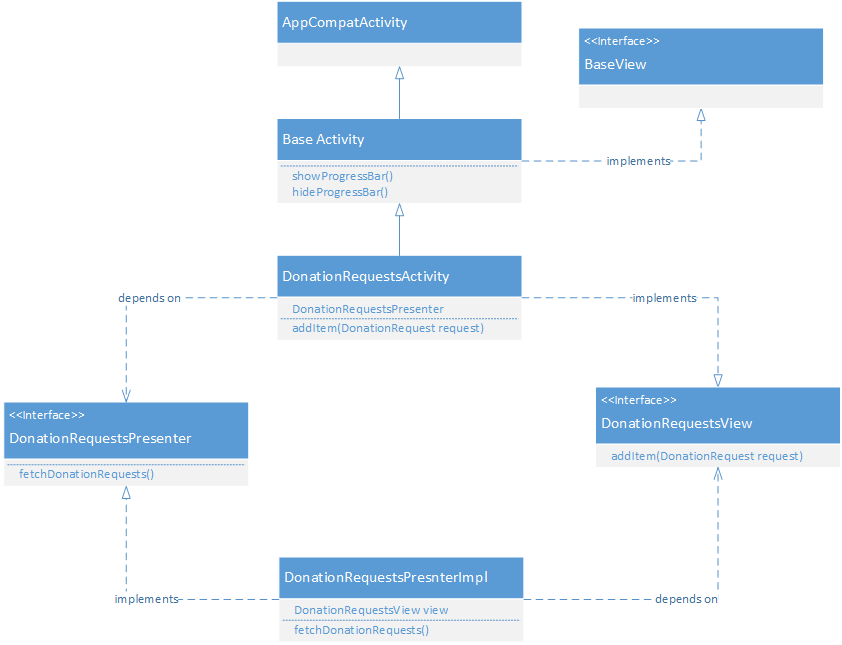
\includegraphics[width=1.1\textwidth]{android_mvp_example_class_diagram.png}
	    \caption{Παράδειγμα διαγράμματος κλάσεων - MVP Android.}
	    \label{fig:android_mvp_example_class_diagram}
	\end{figure}
	
	Σε αυτό το σημείο πρέπει να σημειωθεί ότι για το dependency injection που φαίνεται στο σχήμα \ref{fig:android_mvp_example_class_diagram} έγινε χρήση του dependency injector dagger\cite{daggerAndroid}. 
	
   		\subsubsection{Σύνδεση στην εφαρμογή - Login}
   		
	\begin{figure}[h]
	    \centering
	    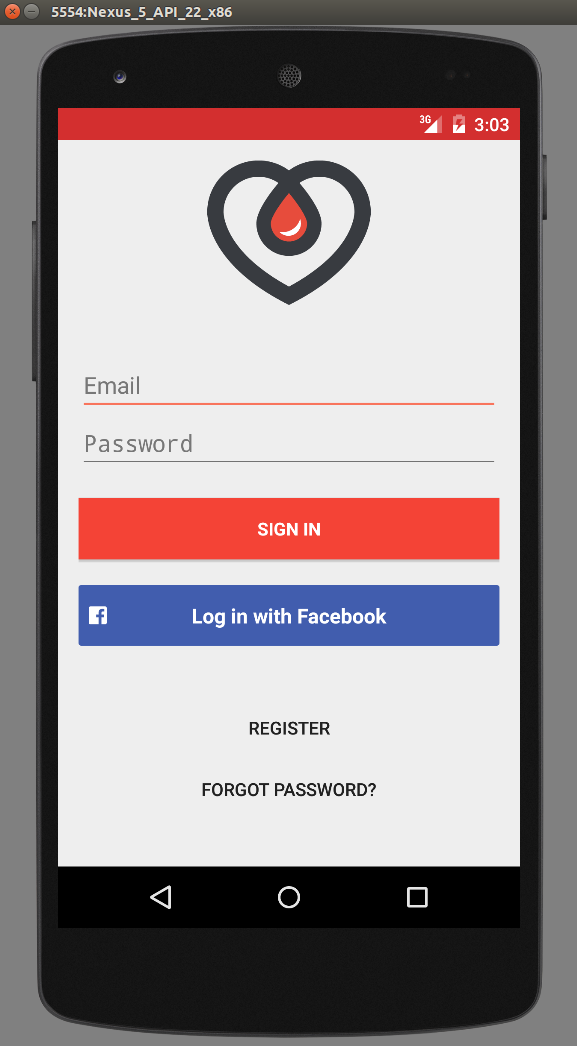
\includegraphics[width=0.6\textwidth]{LoginActivity.png}
	    \caption{Οθόνη σύνδεσης χρήστη στο σύστημα - Android.}
	    \label{fig:LoginActivity}
	\end{figure}
   		
   		
   		Η οθόνη σύνδεσης στο σύστημα υλοποιείται μέσω ενός LoginActivity και ενός LoginPresenter ο οποίος το συνοδεύει. Όπως δείξαμε και στο σχήμα \ref{fig:android_mvp_example_class_diagram}, το LoginPresenter γίνεται inject στο LoginActivity και το LoginView (το οποίο υλοποιείται από το LoginActivity) γίνεται inject στον LoginPresenter αντίστοιχα. Μόλις ο χρήστης συμπληρώσει τα στοιχεία του και κάνει tap στο κουμπί σύνδεσης, το LoginActivity ``περνάει" τα διαπιστευτήρια στον LoginPresenter ο οποίος αρχικώς τα ελέγχει προς ορθότητα. Σε περίπτωση προβλήματος ως προς την ορθότητα ο LoginPresenter λέει στο LoginActivity τι μήνυμα λάθους θα πρέπει να δείξει στον χρήστη. Σε περίπτωση που δεν υπάρχει πρόβλημα ορθότητας, επικοινωνεί με το μοντέλο για να κάνει ταυτοποίηση του χρήστη. Τέλος ο LoginPresenter ενημερώνει το LoginActivity το οποίο με την σειρά του ενημερώνει τον χρήστη με κατάλληλο μήνυμα. 
   		
   		Παρακάτω βλέπουμε ενδεικτικά την κλήση του Presenter από το Activity:
   		\lstinputlisting[language=Java]{attempt_login.java}
		
		Παρακάτω βλέπουμε ενδεικτικά πως ο Presenter λέει στο Activity να δείξει μήνυμα λάθους:
		\lstinputlisting[language=Java]{loginPresenter_error.java}



	- Sign In
	 -Sign Up
	 -Create an Appointment
	 -View History apo tis aimodosies tou
	 -vlepei tis aimodosies genikotera (running, pending)
	 -View badges - rewards
	 -push notification
	
		

%\section{Back-End}
%	\subsection{Parse}
%	\subsection{NodeJS}
%		
%\section{Front-End Cloud App}
%	\subsection{JS}
%	\subsection{jQuery και AngularJS}
%	\subsection{Screenshots}
%	\subsection{Social Networking Integration}
%	\subsection{Testing and Tools}
%		\subsubsection{Unit Testing}
%		\subsubsection{Infrastucture Testing}
%		\subsubsection{Performance Testing}
%		\subsubsection{Browser Compatibility Testing}
%
%\section{Android}
%	\subsection{Activities}
%	\subsection{Screenshots}
%	\subsection{Social Networking Integration}

	\section{Testing and Tools}
	
	\subsection{Android Application Testing}
	
	Στο παρόν κεφάλαιο θα αναφερθούμε αρχικά στο περιβάλλον ελέγχου που μας παρέχει το Android καθώς και στους διαφορετικού τύπους ελέγχου που μπορούμε να εκτελέσουμε. Στην συνέχεια θα αναφερθούμε στους ελέγχους που πραγματοποιήσαμε καθώς και στα αποτελέσματα τους.
	
	Η δυνατότητα αυτοματοποιημένου έλεγχου των εφαρμογών του λειτουργικού Android είναι ιδιαίτερα σημαντική λόγω του μεγάλου αριθμού διαφορετικών συσκευών που υπάρχουν στην αγορά. Είναι αδύνατον να δοκιμάσουμε για μία εφαρμογή όλες τις δυνατές ρυθμίσεις μιας συσκευής, για αυτό αποτελεί συνηθισμένη πρακτική η εκτέλεση δοκιμών με βάση τις πιο συνηθισμένες ρυθμίσεις. Στόχος είναι η επίτευξη ενός υψηλού ποσοστού κάλυψης δοκιμών (test coverage), έτσι ώστε να παράγουμε μια εφαρμογή απαλλαγμένη από σημαντικά σφάλματα αλλά και να διευκολύνουμε την συντήρηση και επέκτασή της στο μέλλον.
	
	Οι δοκιμές στο λειτουργικό σύστημα Android βασίζονται στο JUnit, και μπορούν να χωριστούν σε δύο μεγάλες κατηγορίες όπως φαίνεται στο σχήμα \ref{fig:categories_of_android_tests} ανάλογα με το αν απαιτούν το λειτουργικό συστήματα android ή αν χρειάζονται μόνο την εικονική μηχανή της Java (JVM - Java Virtual Machine) κατά την διάρκεια της εκτέλεσής τους\cite{androidTesting}.
	
	\begin{figure}[h]
	    \centering
	    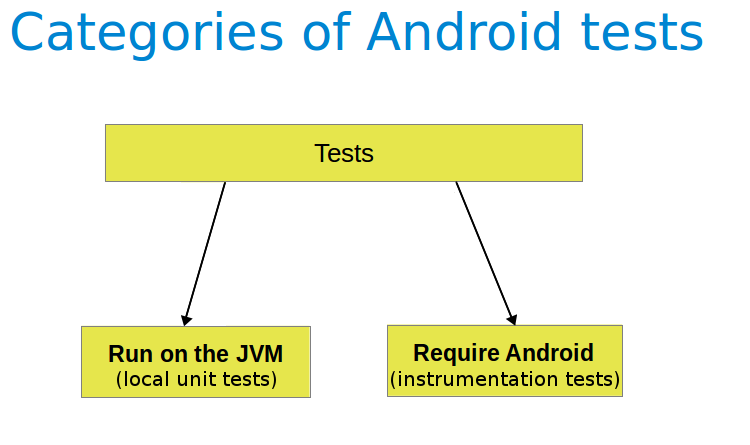
\includegraphics[width=0.7\textwidth]{categories_of_android_tests.png}
	    \caption{ Κατηγορίες δοκιμών στο Android}
	    \label{fig:categories_of_android_tests}
	\end{figure}
	
	Εφόσον είναι εφικτό, είναι πάντα προτιμότερο να τρέχουμε τις δοκιμές στην εικονική μηχανή της Java, δεδομένου ότι απαιτεί πολύ λιγότερο χρόνο σε σχέση με το χρόνο που απαιτείται για την εγκατάσταση και εκτέλεση της εφαρμογής σε μία συσκευή Android. Στην συνέχεια της παρούσας ενότητας η εφαρμογή που δοκιμάζεται θα αποκαλείται \textit{εφαρμογή υπό δοκιμή}.
	
		\subsubsection{Unit Testing (Δοκιμή μονάδας)}
		Έλεγχοι τύπου unit testing χρησιμοποιούνται για την δοκιμή μικρών μεμονωμένων στοιχείων της εφαρμογής, χωρίς να εξετάζεται η αλληλεπίδραση τους με άλλα στοιχεία της εφαρμογής. Δηλαδή όπως δηλώνει και το όνομα τους, εξετάζουν τη συμπεριφορά ενός στοιχείου ως ξεχωριστή μονάδα. Για να γίνει καλύτερα αντιληπτό το παραπάνω, ας υποθέσουμε ότι θέλουμε να δοκιμάσουμε ένα κουμπί το οποίο αναμένουμε να μας μεταφέρει σε μια άλλη οθόνη.  Στα πλαίσια της δοκιμής μονάδας θα γίνει έλεγχος αν η πρόθεση (intent) για αλλαγή οθόνης δημιουργήθηκε σωστά και όχι αν μεταφερθήκαμε στην άλλη οθόνη. Σε περίπτωση όμως που εκτελούσαμε δοκιμές ενσωμάτωσης (instrumentation testing βλ. ενότητα \ref{sssec:instrumentation_testing}) θα έπρεπε να γίνει έλεγχος ότι η επόμενη οθόνη ξεκίνησε όπως αναμέναμε.
		
		Τα Unit tests χρησιμοποιούν το JUnit test framework και δεν πρέπει να χρησιμοποιούν λειτουργίες από το Android API έτσι ώστε να είναι σε θέση να τρέξουν στην εικονική μηχανή της Java (JVM) κάτι το οποίο απαιτεί πολύ λιγότερο χρόνο σε σχέση με τον χρόνο τον οποίο θα χρειάζονταν για να τρέξουν σε περιβάλλον Android. Κάθε εξάρτηση από το λειτουργικό Android θα πρέπει να αντικατασταθεί στον κώδικα που θέλουμε να δοκιμάσουμε με κάποιο mocking framework όπως είναι το Mockito. 
		
		Παρακάτω βλέπουμε ένα απλό JUnit test που φτιάξαμε με σκοπό να δοκιμάσουμε την λειτουργία της συνάρτησης που ελέγχει την εγκυρότητα του κωδικού χρήστη.
		
		\lstinputlisting[language=Java]{ValidatorTest.java}  

		\subsubsection{Instrumentation Testing}\label{sssec:instrumentation_testing}

		Όταν θέλουμε να δοκιμάσουμε κλάσεις και λειτουργίες της εφαρμογής οι οποίες αλληλεπιδρούν με το λειτουργικό Android τότε δημιουργούμε τις λεγόμενες δοκιμές ενσωμάτωσης (instrumentation tests). Το Android API για δοκιμές παρέχει στον προγραμματιστή άγκιστρα (hooks) μέσω των οποίων μπορεί να αλληλεπιδράσει με τον κύκλο ζωής των στοιχείων λογισμικού και της εφαρμογής. Αυτά τα άγκιστρα απαρτίζουν το instrumentation API και επιτρέπουν στις δοκιμές να ελέγχουν γεγονότα από τον κύκλο ζωής (life cycle events) και την αλληλεπίδραση του χρήστη.

		Υπό κανονικές συνθήκες ένα στοιχείο του Android ακολουθεί έναν κύκλο ζωής που έχει καθοριστεί από το σύστημα βάση της αλληλεπίδρασης του με τον χρήστη. Για παράδειγμα, όταν δημιουργείται μια πρόθεση (intent) για έναρξη κάποιου Activity, καλείται η μέθοδος onCreate() του εν λόγω Activity. Στην συνέχεια αν ο χρήστης ανοίξει κάποια άλλη εφαρμογή, καλείται η μέθοδος onDestroy() του Activity . Το instrumentation API αν και δεν επιτρέπει στον προγραμματιστή να καλέσει αυτές τις μεθόδους απευθείας, του επιτρέπει να εξομοιώσει πλήρως την συμπεριφορά ενός χρήστη η οποία προκαλεί τέτοια γεγονότα. Για παράδειγμα επιτρέπει στον προγραμματιστή να στείλει γεγονότα πλήκτρων ή αφής, ελέγχοντας με αυτό τον τρόπο τον κύκλο ζωής της υπό δοκιμής εφαρμογής\cite{androidTestingBook}.

		Τα instrumentation tests δεν γίνεται να τρέξουν στο JVM αλλά χρειάζονται περιβάλλον με λειτουργικό σύστημα Android. Μπορούν να τρέξουν είτε σε πραγματική συσκευή Android η οποία έχει συνδεθεί με τον υπολογιστή στον οποίο γίνεται η ανάπτυξη, είτε σε εικονική συσκευή Android. Δεδομένου του πλήθους των συσκευών που τρέχουν το λειτουργικό σύστημα Android, και συνυπολογίζοντας τις διάφορες εκδόσεις που μπορεί να τρέχει κάθε συσκευή, κάθε δοκιμή θα πρέπει να γίνεται με χρήση εξομοίωσης σε διάφορα επίπεδα API αλλά και μεγέθη οθονών. Για παράδειγμα αν η εφαρμογή υποστηρίζει επίπεδο API μεγαλύτερο του 14 θα πρέπει να γίνει έλεγχος για κάθε API μεγαλύτερο του 14 με τουλάχιστον 2 διαφορετικά μεγέθη οθόνης για κάθε API. 
		
		Όπως γίνεται εμφανές από τα παραπάνω το τρέξιμο των instrumentation tests αποτελεί μια ιδιαίτερα χρονοβόρα διαδικασία. Για την εξομάλυνση αυτού του προβλήματος υπάρχουν υπηρεσίες μέσω των οποίων οι δοκιμές μπορούν να γίνουν στο υπολογιστικό νέφος. Παρακάτω βλέπουμε ένα παράδειγμα δοκιμών instrumentation που φτιάξαμε για να ελέγξουμε την λειτουργία επαναφοράς κωδικού.
		
		\lstinputlisting[language=Java]{ResetPassword.java}
		
		\subsubsection{Performance Testing}
		\subsubsection{Android API Level compatibility testing}
		\subsection{NodeJs Testing}
		
		\subsubsection{Browser Compatibility Testing}


\graphicspath{ {Figures/interoperability/} }
\chapter{Διασυνδεσιμότητα}\label{ch:Interoperability}
\section{Απαιτήσεις}

\section{Πρωτόκολλα επικοινωνίας}


	\subsection{Το πρότυπο Health Level Seven (HL7)}
		\subsubsection{Ο Οργανισμός Health Level Seven (HL7)}
		Το πρότυπο HL7 το οποίο έχει δημιουργηθεί από τον ομώνυμο οργανισμό Health Level Seven, ο οποίος αποτελεί μη κερδοσκοπικό οργανισμό με έτος ίδρυσης 1987 στις Ηνωμένες Πολιτείες της Αμερικής\cite{HL7Organization}\cite{blobel2003hl7}. Ο οργανισμός HL7 συστάθηκε με στόχο την δημιουργία παγκοσμίως αναγνωρισμένων και αξιόπιστων προτύπων για την ανταλλαγή ιατρικών δεδομένων μεταξύ ενδιαφερομένων φορέων στον τομέα της ιατρικής περίθαλψης. Τα δεδομένα αυτά αφορούν τόσο την κλινική φροντίδα των ασθενών όσο και το κομμάτι της διαχείρισης, οργάνωσης, αξιολόγησης και επέκτασης των υπηρεσιών Ιατρικής φροντίδας.

Ο μη κερδοσκοπικός οργανισμός Health Level Seven αποτελεί έναν από τους βασικότερους φορείς για τη διασφάλιση και διαλειτουργικότητα, μεταξύ των συστημάτων παροχής υπηρεσιών Ηλεκτρονικής Ιατρικής Φροντίδας (e-health). Αριθμεί πολυποίκιλα μέλη σε περισσότερες από 55 χώρες μεταξύ των οποίων δημόσιους και ιδιωτικούς φορείς Υγείας, εταιρείες παροχής Ιατρικού λογισμικού, εταιρείες παροχής Ιατρικού εξοπλισμού, ειδικούς συμβούλους, εμπειρογνώμονες, ασφαλιστικούς φορείς κτλ\cite{HL7Organization}. Είναι δεδομένο άλλωστε ότι ο χώρος της Υγείας περιλαμβάνει αρκετούς ενδιαφερόμενους φορείς, καθιστώντας απαραίτητη τη χρήση προτύπων και αντίστοιχων αρχιτεκτονικών κατευθύνσεων ώστε να επιτευχθεί η διαλειτουργικότητα σε ένα ενοποιημένο σύστημα Ηλεκτρονικής Υγείας στο οποίο θα συμμετέχουν οι εμπλεκόμενοι φορείς, ο καθένας με το δικό του ρόλο. Επίσης αξίζει να σημειωθεί ότι έχει ο οργανισμός HL7 έχει τοπικά υποκαταστήματα σε όλες σχεδόν τις χώρες της Ευρώπης, στην Αυστραλία - Νέα Ζηλανδία, στην Ασία, στις Ηνωμένες Πολιτείες της Αμερικής και στη ζώνη του Ειρηνικού. Στην Ελλάδα ιδρύθηκε και λειτουργεί από το 2003 το παράρτημα (μη κερδοσκοπικού χαρακτήρα) του διεθνούς οργανισμού Health Level Seven (HL7) με την επωνυμία "HL7 Hellas". Ο ιδρυτικός πυρήνας περιλαμβάνει δεκαπέντε (15) διακεκριμένα ονόματα φορέων τόσο από τον Πανεπιστημιακό όσο και από τον χώρο των εταιριών Ιατρικής Πληροφορικής και Τεχνολογίας\cite{HL7Hellas}.
		\subsubsection{Το πρότυπο HL7, έκδοση 2}
		Το πιο ευρέως χρησιμοποιούμενο πρότυπο επικοινωνίας και διαλειτουργικότητας συστημάτων Ηλεκτρονικής Υγείας (healthcare interoperability standard) είναι η έκδοση 2 του προτύπου HL7 (HL7 v2). Χαρακτηριστικό παράδειγμα αποτελεί η περίπτωση των Ηνωμένων Πολιτειών της Αμερικής στις οποίες βρίσκει χρήση σε ποσοστό 95\% των νοσοκομειακών συστημάτων\cite{benson2012principles}.
		
		Η έκδοση 2 του προτύπου HL7 εισήχθηκε τον Οκτώβριο του 1987, μόλις ένα χρόνο μετά την εμφάνιση της έκδοσης 1 και βρίσκεται υπό συνεχή ανάπτυξη εδώ και πάνω από 25 χρόνια. Τη στιγμή της συγγραφής της παρούσας διπλωματικής εργασίας, τελευταία έκδοση του HL7 V2 είναι η 2.7, η οποία έλαβε και έγκριση ως πρότυπο ANSI το έτος 2011\cite{HL7Version27}. Η έκδοση αυτή ορίζει διάφορους τύπους ηλεκτρονικών μηνυμάτων για την υποστήριξη διοικητικών, λογιστικών, οικονομικών, καθώς και ιατρικών διαδικασιών. Μία από τις βασικές απαιτήσεις κατά την εξέλιξη του HL7 V2 είναι η διασφάλιση ότι τα μηνύματα που έχουν δημιουργηθεί βάσει παλαιότερων εκδόσεων συνεχίζουν να είναι έγκυρα σε περιβάλλοντα που έχουν εφαρμόσει νεότερες εκδόσεις του προτύπου, οι οποίες έχουν σχεδιαστικά προσθετικά των προηγούμενων (backward compatibility). Για παράδειγμα μια εφαρμογή η οποία αποκωδικοποιεί μηνύματα της έκδοσης 2.5 πρέπει να είναι σε θέση να αποκωδικοποιήσει και μηνύματα της έκδοσης 2.4. Οι κύριοι λόγοι για τους οποίους οι παλαιότερες εκδόσεις του HL7 V2 χρησιμοποιούνται ακόμα σε τόσο μεγάλο βαθμό είναι οι παρακάτω:
		\begin{enumerate}
			\item Δεν υπάρχει ιδιαίτερο κίνητρο για αναβάθμιση δεδομένου ότι το όφελος από την επένδυση για αντικατάσταση της υπάρχουσας διεπαφής με κάποια καινούργια είναι αρκετά χαμηλό (low return on investment).
			\item Δεδομένου της ευαίσθητης φύσης αλλά και της απαίτησης συνεχούς λειτουργίας (100\% uptime) των συστημάτων υγείας, το ρίσκο αποτυχίας της αλλαγής λειτουργεί συνήθως ως αποτρεπτικός παράγοντας.
		\end{enumerate}		 
		
		Αν και όπως προαναφέραμε το πρότυπο HL7 V2 χρήζει ευρείας αποδοχής δεν είναι χωρίς τα ελαττώματα του, συγκεκριμένα\cite{bourquard2015standards}:
		\begin{enumerate}
			\item Δεν υπάρχει κάποιο σαφώς καθορισμένο μοντέλο αναφοράς της πληροφορίας που ανταλλάσσεται μέσω των μηνυμάτων αλλά ούτε και τρόπος να αναπαρασταθεί η σχέση μεταξύ των δεδομένων.
			\item Χρησιμοποιεί μια εξαιρετικά εδική σύνταξη στα μηνύματα με άμεσο αποτέλεσμα να είναι ιδιαιτέρως δύσκολη η εκμάθηση αλλά και η υλοποίηση του προτύπου.
			\item Αν και τα πολλά προαιρετικά χαρακτηριστικά που διαθέτει του παρέχουν μεγάλο βαθμό ευελιξίας, δημιουργούν προβλήματα ως προς τον έλεγχο της συμμόρφωσης προς το πρότυπο των διαφόρων υλοποιήσεων. Ως άμεσο αποτέλεσμα χρήζει μεγάλης προσπάθειας η εξασφάλιση ότι δύο εφαρμογές που θα επικοινωνήσουν μεταξύ τους, κάνουν χρήση των ίδιων χαρακτηριστικών.
		\end{enumerate}
		
		Τα μηνύματα HL7 V2 αποτελούνται από μια ορισμένη σειρά τμημάτων (segments). Κάθε τμήμα περιέχει κάποια πεδία τα οποία είναι επίσης σε κάποια προκαθορισμένη σειρά. Κάθε πεδίο έχει προκαθορισμένους τύπους δεδομένων (data types), ο οποίοι μπορεί να είναι οι ακόλουθοι\cite{dolin2001hl7}:
		\begin{itemize}
			\item Απλός τύπος μιας τιμής, παραδείγματος χάριν text ή date.
			\item Σύνθετος τύπος δεδομένων ο οποίος αποτελείται από πολλαπλά επί μέρους συστατικά (components). Κάθε συστατικό έχει έναν δικό του προκαθορισμένο τύπο δεδομένων ο οποίος με τη σειρά του μπορεί να είναι επίσης απλός ή σύνθετος τύπος δεδομένων. Καθαυτό τον τρόπο οδηγούμαστε στην δημιουργία υποσυστατικών (subcomponents).
		\end{itemize}
		
		Τα μηνύματα του προτύπου HL7 v2 μεταφέρονται με την πυροδότηση κάποιου γεγονότος. Κάθε μήνυμα αντιστοιχείται σε κάποια γενική κατηγορία, εντός της οποίας ανήκει. Παραδείγματος χάριν, τα μηνύματα τα οποία έχουν σχέση με την διαχείριση των ασθενών ανήκουν στην κατηγορία "ADT" (από τα αρχικά των λέξεων admission, discharge, transfer). Παρακάτω στον πίνακα \ref{tab:HL7_V2_message_types} με κάποια παραδείγματα τύπων μηνυμάτων:
		
	\begin{table}[h]
		\begin{center}
		    \begin{tabular}{|l|l|}
		    \hline
		    \rowcolor{grayy}
		    \textbf{Τιμή} & \textbf{Περιγραφή}
		    \\ \hline
		     ACK & Μήνυμα επιβεβαίωσης (acknowledge)
		     \\ \hline
		     ADT & Μήνυμα για τη διαχείριση των ασθενών
		     \\ \hline
		     BTS & Μετάγγιση αίματος (Blood product transfusion)
		     \\ \hline
		     PIN & Πληροφορίες ασφάλισης ασθενούς (Patient insurance information)
		     \\ \hline
		    \end{tabular}
		    \caption{Παραδείγματα τύπων μηνυμαων HL7 V2}
			\label{tab:HL7_V2_message_types}
		\end{center}
	\end{table}
	
	Όπως προαναφέρθηκε παραπάνω πριν την δημιουργία κάποιου μηνύματος θα πρέπει να έχει προηγηθεί κάποιο γεγονός πυροδότησης. Κάθε γεγονός πυροδότησης ανήκει σε κάποιον τύπο μηνύματος. Για παράδειγμα στον τύπο μηνύματος ADT ανήκει το γεγονός A01 το οποίο αναφέρεται στην εισαγωγή ή επίσκεψη του ασθενή και το Α02 το οποίο αναφέρεται στην μεταφορά του ασθενή. Για να επιτευχθεί ο πλήρης καθορισμός ενός μηνύματος θα πρέπει να γίνει συνδυασμός τόσο του τύπου μηνύματος όσο και του γεγονότος πυροδότησης. Βάση των παραδειγμάτων που έχουμε αναφέρει παραπάνω, ένα πλήρες όνομα μηνύματος θα ήταν το $ADT^A02$. Ο χαρακτήρας $"^"$ χρησιμοποιείται έτσι ώστε να διαχωρίσουμε τα διάφορα συστατικά ενός πεδίου. Δεδομένου της υψηλής σημασίας που παίζουν οι χαρακτήρες οριοθέτησης στην σωστή αποκωδικοποίηση και δημιουργία του μηνύματος, παρουσιάζουμε στον πίνακα \ref{tab:HL7_delimeters} τους χαρακτήρες οριοθέτησης:
	
	\begin{table}[h]
		\begin{center}
		    \begin{tabular}{|c|l|}
		    \hline
		    \rowcolor{grayy}
		    \textbf{Χαρακτήρας} & \textbf{Χρήση}
		    \\ \hline
		     | & Διαχωρισμός πεδίων
		     \\ \hline
		     \^{} & Διαχωρισμός συστατικών
		     \\ \hline
		     \~{} & Διαχωρισμός επαναλήψεων
		     \\ \hline
		     \textbackslash & Χαρακτήρας διαφυγής
		     \\ \hline
		     \& & Διαχωρισμός υποσυστατικών
		     \\ \hline
		     $<CR>$ & Τερματισμός τμημάτων
		     \\ \hline
		    \end{tabular}
		    \caption{Χαρακτήρες οριοθέτησης του προτύπου HL7 V2}
			\label{tab:HL7_delimeters}
		\end{center}
	\end{table}
	
	\textbf{ΠΙΝΑΚΕΣ ΓΙΑ HL7 V2}
		
		\subsubsection{Το πρότυπο HL7, έκδοση 3}
	\subsection{CDA Documents}
	

		
\section{Δυνατότητες διασύνδεσης με άλλα υποσυστήματα}

	\subsection{Ηλεκτρονική Συνταγογράφηση}
	
		Η διαδικασία της συνταγογράφησης φαρμάκων μπορεί να είναι ιδιαίτερα περίπλοκη και επιρρεπής σε λάθη, με
δυσμενείς επιπτώσεις για την ασφάλεια των ασθενών. Η πρόληψη των επιπλοκών που μπορούν να προκύψουν λόγω ακατάλληλης συνταγογράφησης είναι μία πρόκληση που αντιμετωπίζει το σύστημα υγείας σε παγκόσμιο επίπεδο. Οι λανθασμένες φαρμακευτικές αγωγές, οι παρενέργειες των φαρμάκων και η αποτυχία σωστής συνταγογράφησης που να συντελέσει στην θεραπεία του ασθενούς εκτός του γεγονότος ότι αποτελεί απειλή για την ασφάλεια του, οδηγεί σε σημαντικές δαπάνες για τα συστήματα υγειονομική περίθαλψης. Οι πληροφορίες σχετικά με το ιστορικό του ασθενούς, τις αλλεργίες, τις παρελθοντικές και τις τρέχουσες φαρμακευτικές αγωγές καθώς και τα εργαστηριακά αποτελέσματα του είναι άκρως απαραίτητα ώστε οι κλινικοί ιατροί να συνταγογραφήσουν την κατάλληλη φαρμακευτική αγωγή, αλλά είναι συχνά δεν είναι διαθέσιμα. \cite{prescribingErrors} Στην Ελλάδα ειδικότερα, υφίσταται το πρόβλημα της αλόγιστης ή πλασματικής συνταγογράφησης με αποτέλεσμα να  χρειάζονται μέτρα για την επαναφορά της αξιοπιστίας της διαδικασίας.  Χαρακτηριστικό παράδειγμα είναι τα στοιχεία του Υπουργείου Υγείας και Κοινωνικής Ασφάλισης, με βάση τα οποία το έτος 2009 εκτελεστήκαν στην Ελλάδα περίπου 100 εκατομμύρια ετησίως ενώ αντίστοιχα στην Δανία εκτελέστηκαν μόνο 15 εκατομμύρια συνταγές.


		Με τον όρο ηλεκτρονική συνταγογράφηση (e-prescription) σύμφωνα με το Εθνικό Σύστημα Υγείας στην Αγγλία αναφερόμαστε στην αξιοποίηση των ηλεκτρονικών συστημάτων για την διευκόλυνση και την ενίσχυσης της επικοινωνίας μίας ιατρικής εντολής ή συνταγής, βοηθώντας στην επιλογή, τη διαχείριση και την προμήθεια ενός φαρμάκου μέσω της γνώσης και υποστήριξης αποφάσεων, παρέχοντας μια διαδρομή ελέγχου για το σύνολο της διαδικασίας χρήσης των φαρμάκων.  Τα συστήματα ηλεκτρονικής συνταγογράφησης που προσφέρουν ηλεκτρονική υποστήριξη στους κλινικούς ιατρούς έχουν σχεδιαστεί για να βοηθήσουν στην περίπλοκη διαδικασία της συνταγογράφησης. \cite{Kierkegaard2013} Επιτρέπουν σε έναν γιατρό, έναν φαρμακοποιό, μία νοσηλεύτρια να διαβιβάσει χωρίς σφάλματα, ακριβείς και κατανοητές συνταγές ηλεκτρονικά, μέσα από τον φορέα παροχής υπηρεσιών υγείας, στο φαρμακείο.  \cite{eprescr}
		
		
		Τα συστήματα ηλεκτρονικής συνταγογράφησης μπορεί να έχουν λειτουργικές δυνατότητες για την παροχή βασικής υποστήριξης αποφάσεων, όπως ο έλεγχος για τυχόν αλλεργίες στα φάρμακα, βασικές κατευθυντήριες γραμμές για τη δοσολογία, τεστ για πιθανές αντιδράσεις μεταξύ φαρμάκων κ.λ.π. Τα συστήματα αυτά είναι ιδιαίτερα χρήσιμα στο τεχνικό κομμάτι της συνταγογράφησης κατάλληλων φαρμάκων, καθώς προσφέρουν λειτουργίες όπως ο υπολογισμός της σωστής δόσης ή ο εντοπισμός αλληλεπιδράσεων μεταξύ των φαρμάκων. \cite{Kart2008}

		Τα συστήματα ηλεκτρονικής συνταγογράφησης χωρίζονται σε δύο κατηγορίες:
		
		\begin{itemize}
		
		\item Τα αυτόνομα συστήματα (stand alone systems). Πρόκειται για λειτουργικά συστήματα τα οποία είναι εγκατεστημένα στους ηλεκτρονικούς υπολογιστές  και χρησιμοποιούνται είτε αυτόνομα είτε μέσω σύνδεσης στο διαδίκτυο.  Τα συστήματα αυτά χρησιμοποιούνται κυρίως για τον έλεγχο θεμάτων ασφάλειας και γίνεται προσπάθεια αντικατάστασης τους από τα ολοκληρωμένα συστήματα συνταγογράφησης.

		\item Τα ολοκληρωμένα συστήματα συνταγογράφησης (Electronic Health Record, EHR Systems). Στα συστήματα αυτά ο ιατρός έχει στην διάθεση του όλο το ιστορικό του ασθενούς, τα αποτελέσματα των εξετάσεων του και τα χρησιμοποιεί για να βοηθηθεί στην επιλογή της κατάλληλης δραστικής ουσίας. Οι συναγερμοί ασφαλείας στην περίπτωση αυτή είναι πιο εξειδικευμένοι και ακριβείς.  

		\end{itemize}
		

		Συνοπτικά τα συστατικά της ηλεκτρονικής συνταγογράφησης μπορούν να κατηγοριοποιηθούν σε βασικές δυνατότητες συνταγογράφησης, πληροφορίες για το πλάνο υγείας και τις κλινικές ειδοποιήσεις (clinical alerts).  Οι δυνατότητες συνταγογράφησης περιλαμβάνουν μια λίστα φαρμάκων, οδηγίες για τους ασθενείς, τον αριθμός των εγκεκριμένων ποσοτήτων, σχόλια του γιατρού που συνταγογραφεί προς τον φαρμακοποιό, καθώς και το πεδίο PRN. Οι πληροφορίες για το πλάνο υγείας του ασθενούς περιλαμβάνουν την ιατρική ασφάλεια που έχει και το ιστορικό των φαρμακευτικών αγωγών. Τέλος, οι κλινικές ειδοποιήσεις  βασίζονται στα δημογραφικά στοιχεία και στα στοιχεία του ιατρικού ιστορικού του ασθενούς και περιλαμβάνουν τις αντιδράσεις μεταξύ των φαρμάκων, τις αλλεργίες, τις προειδοποιήσεις για συγκεκριμένες ηλικιακές ομάδες και την κατάλληλη προσαρμογή της δόσης με βάση το βάρος του ασθενούς. \cite{prescribing} 
		
		
		Τα βασικά συστατικά ενός συστήματος ηλεκτρονικής συνταγογράφησης είναι \cite{Grossman2012}:

		\begin{itemize}

		\item Ο παραπέμπων ιατρός. Ο θεράπων ιατρός είναι ο κύριος χρήστης  του συστήματος. Για την σύνδεση του στο σύστημα ακολουθείται μιας διαδικασία επαλήθευσης ώστε να επιβεβαιωθεί η ταυτότητά του. 
Οι αναζητήσεις του θεράποντα ιατρού στην βάσης δεδομένων που περιέχει τους φακέλους των ασθενών πραγματοποιείται με τη χρήση ειδικών πληροφοριών για τον ασθενή, συνήθως το ΑΜΚΑ για Ελλάδα ή τον αριθμό κοινωνικής ασφάλισης (social security number) στον εξωτερικό. Μόλις προσπελαστεί το σωστό αρχείο του ασθενούς, ο ιατρός εξετάζει τις ιατρικές πληροφορίες που περιέχει και προσθέτει ή ενημερώνει μία συνταγή στον ιατρικό φάκελο.
		
		\item Ο κόμβος συναλλαγών. Αποτελεί τον κοινό σύνδεσμο μεταξύ όλων των φορέων (παραπέμπων ιατρός και φαρμακείο). Αποθηκεύει και διατηρεί ένα κύριο κατάλογο των ασθενών για να υπάρχει η δυνατότητα γρήγορης πρόσβασης στις ιατρικές πληροφορίες των ασθενών, καθώς και στην λίστα των φαρμακείων. Όταν ο παραπέμπων ιατρός ανεβάσει κάποια νέα συνταγή στον φάκελο του ασθενούς, τότε αυτή μεταφέρεται αυτόματα και στον κόμβο συναλλαγών. Ο κόμβος συναλλαγών θα στείλει αυτόματα τις πληροφορίες  με στο κεντρικό σύστημα διαχείρισης το οποίο θα απαντήσει με πληροφορίες σχετικά με την καταλληλότητα του ασθενή και το ιστορικό των φαρμακευτικών αγωγών του.  Ο κόμβος συναλλαγών έπειτα στέλνει τις πληροφορίες στον ιατρό έτσι ώστε να έχει τις απαραίτητες πληροφορίες που του χρειάζονται και να ολοκληρώσει και να εγκρίνει την συνταγή. 
		
		\item Το κεντρικό σύστημα διαχείρισης δεδομένων, στο οποίο βρίσκονται όλα τα στοιχεία ιατρικού φακέλου που ελέγχει την καταλληλότητα του ασθενή καθώς και της συνταγής. Το κεντρικό σύστημα διαχείρισης δεδομένων επικοινώνει με τον ιατρό και το φαρμακείο.
		
		\item Το φαρμακείο που έχει εγκατεστημένο το λογισμικό της ηλεκτρονικής συνταγογράφησης. Το φαρμακείο ανακτά την συνταγή από  το κεντρικό σύστημα διαχείρισης συναλλαγών μέσω του κόμβου συναλλαγών και έχει επιπλέον την ικανότητα να επικοινωνήσει με τον ιατρό και να τον ενημερώσει ότι η παραγγελία εκτελέστηκε. 
		
		\end{itemize}
		
		
		
		\subsubsection{Ηλεκτρονική Συνταγογράφηση στην Ελλάδα}
		
		Η ηλεκτρονική συνταγογράφηση στην Ελλάδα βασίζεται στις οδηγίες του νόμου 3892/2010 (ΦΕΚ 189 Α) «Ηλεκτρονική καταχώριση και εκτέλεση ιατρικών συνταγών και παραπεμπτικών ιατρικών εξετάσεων». Σε αυτόν το νόμο καταγράφονται τα ζητήματα ηλεκτρονικής συνταγογράφησης και τα ζητήματα των ηλεκτρονικών παραπεμπτικών.
		
		Ο υπεύθυνος φορέας στην Ελλάδα είναι η Γενική Γραμματεία Κοινωνικών Ασφαλίσεων του Υπουργείου Εργασίας, Κοινωνικής Ασφάλισης και Πρόνοιας. Το σύστημα υποστηρίζεται ηλεκτρονικά από την Ηλεκτρονική Διακυβέρνηση Κοινωνικής Ασφάλισης (ΗΔΙΚΑ Α.Ε.). Η ΗΔΙΚΑ αποτελεί μια ανώνυμη, μη κερδοσκοπικού χαρακτήρα του δημοσίου την οποία αποζημιώνουν οι εξυπηρετούμενοι φορείς για τις υπηρεσίες του παρέχει, όπως για παράδειγμα το έργο μισθοδοσίας των φορέων.  \cite{idika}
		
		Με τον όρο ηλεκτρονική συνταγογράφηση αναφερόμαστε στη παραγωγή, στην διακίνηση και στον έλεγχο των ιατρικών συνταγών και των παραπεμπτικών για ιατρικές πράξεις, με τη χρήση τεχνολογίας ηλεκτρονικών υπολογιστών και επικοινωνιών, έτσι ώστε να διασφαλίζεται η ασφάλεια, η εγκυρότητα και η διαφάνεια στις πληροφορίες που διακινούνται. Ουσιαστικά, το σύστημα περιλαμβάνει ένα αριθμό από διαδικασίες που σχετίζονται με τη δημιουργία, την εκτέλεση, τη διαχείριση, τον έλεγχο, την εκκαθάριση και την εξόφληση μιας φαρμακευτικής συνταγής ή ενός παραπεμπτικού για ιατρικές πράξεις. Διέπει όλα τα συστήματα και τις τοποθεσίες που εμπλέκονται όπως τα τακτικά ιατρεία των νοσοκομείων ή τα ιδιωτικά ιατρεία, τα κέντρα υγείας, τις κλινικές, τα διαγνωστικά κέντρα, τα φαρμακεία και τα ασφαλιστικά ταμεία.


		
		Το ολοκληρωμένο σύστημα ηλεκτρονικής συνταγογράφησης στην Ελλάδα εξυπηρετεί τους εξής σκοπούς:
		
		\begin{itemize}

		\item  Βοηθά στον αποτελεσματικό εκσυγχρονισμό του συστήματος της φαρμακευτικής περίθαλψης. Οι χειρόγραφες συνταγές έχουν αντικατασταθεί από τις ηλεκτρονικές και η διαδικασία έχει αυτοματοποιηθεί.
		 
		\item Συντελεί στην ταυτοποίηση και τον έλεγχο των εμπλεκομένων για να διασφαλίσει την ακεραιότητα της διαδικασίας και την ευρεία και επιτυχημένη επιχειρησιακή λειτουργία της ηλεκτρονικής συνταγογράφησης.
		
		\item Βελτιώνει την ασφάλεια και την ποιότητα της φροντίδας του ασθενούς. Με την αύξηση του όγκου των φαρμάκων και της πολυπλοκότητα των ιατρικών αναγκών των ασθενών, εφίσταται αυξημένος κίνδυνος σφαλμάτων και παρενεργειών. Η ηλεκτρονική συνταγογράφηση μπορεί να βελτιώσει την ασφάλεια και την ποιότητα της φροντίδας του ασθενούς και να μειώσει τον αριθμό των λαθών
		
		\item Εισάγει και αξιοποιεί τις λειτουργίες της ηλεκτρονικής συνταγογράφησης στην καθημερινή πρακτική.

		\end{itemize}

	\subsubsection{E-prescription }
	
		Το ελληνικό σύστημα ηλεκτρονικής συνταγογράφησης,  το επονομαζόμενο e-precription, καθιερώθηκε το 2013. Πλέον καλύπτει περισσότερο  από το 95\% του συνόλου των συνταγών που γράφονται . Το e-precription δημιουργήθηκε με σκοπό να παρέχει τις εξής λειτουργίες: την ηλεκτρονική καταχώρηση και διαχείριση των συνταγών, την ενίσχυση της γνώσης μέσω της δυνατότητας άμεσης πρόσβασης στις πληροφορίες των φαρμάκων, την υποστήριξη λήψης αποφάσεων καθώς βοηθά την επιλογή των φαρμάκων με διάφορες ειδοποιήσεις, την υποστήριξη κατά την διοίκηση, την δημιουργία ηλεκτρονικών συνδέσμων μεταξύ των νοσοκομείων και των φαρμακείων, τις βελτιώσεις στις ήδη υπάρχουσες εργασιακές διαδικασίες, και τέλος την ανάπτυξης μιας διαδρομή ελέγχου για το σύνολο της χρήσης των φαρμάκων.  \cite{miller}
		
		Το e-prescription πραγματοποιεί την ηλεκτρονική επεξεργασία των συνταγών για όλους τους ασθενείς, οι οποίοι είναι ασφαλισμένοι σε κάποιον από τους εθνικούς φορείς ασφαλίσεων.Το σύστημα εστιάζει ιδιαιτέρως στην βελτίωση της ασφάλειας των ασθενών, την καλύτερη αξιοποίηση των πόρων και στην διαλειτουργικότητα με άλλα εθνικά ή ευρωπαϊκά συστήματα. Είναι διαθέσιμο μέσω του διαδικτύου (internet) και αποτελεί ένα αυτόνομο ηλεκτρονικό σύστημα εισόδου στο οποίο κάθε υποβολή συνταγής είναι ασφαλής και αναγνωρίζεται από έναν μοναδικό αριθμό. Στο σχήμα \ref{fig:prescr} απεικονίζεται η συνολική δομή του συστήματος. \cite{pangalos}
		
		Ο θεράπων ιατρός δημιουργεί τις συνταγές οι οποίες αποθηκεύονται στην εθνική βάση του συστήματος e-prescription , η οποία βρίσκεται στην ΗΔΙΚΑ. \cite{idika}Όταν ένα φαρμακείο θέλει να εκτελέσει μία συνταγή την  "διαβάζει" από την κεντρική βάση. Οι πληροφορίες ου βρίσκονται στην βάση δεδομένων είναι διαθέσιμες (μέσω ασφαλούς on-line πρόσβασης, ή εξειδικευμένων περιοδικών αναφορών) σε όλα τα σχετικά και ενδιαφερόμενα μέρη (Οργανισμοί Ασφάλισης Υγείας, Υπουργείο Υγείας, εποπτικές αρχές, κλπ). Οι συνταγές που έχουν εκτελεστεί από τα φαρμακεία  ελέγχονται από τους οργανισμούς ασφάλισης, ενώ το σύστημα e-prescription χρησιμοποιείται για να διασταυρώνονται οι έλεγχοι. \cite{papala}

	Η εφαρμογή του e-prescription είναι μία διαδικτυακή εφαρμογή. Στο σύστημα έχουν πρόσβαση μόνο εξουσιοδοτημένοι χρήστες (ιατροί, φαρμακοποιοί, κλπ), οι οποίοι αναγνωρίζονται και αποκτούν άδεια πρόσβασης μετα την χρήση κατάλληλων διαπιστευτηρίων. για χωροθέτηση και αδειοδότηση.
	
	Ο θεράπων ιατρός δημιουργεί συνταγές, οι οποίες παρέχουν όλες τις απαραίτητες πληροφορίες τόσο για τους ιατρικούς όσο και για τους διοικητικούς σκοπούς.  Στις πληροφορίες αυτές συμπεριλαμβάνεται ο αριθμός κοινωνικής ασφάλισης  του ασθενούς και του ιατρού , ο κωδικός της διάγνωσης (που κωδικοποιείται στο ICD-10), τα στοιχεία του καθορισμένου φαρμάκου (ποσότητα, δοσολογία, κ.λ.π.), το ποσοστό συμμετοχής του ασθενή στην πληρωμή του φαρμάκου και άλλα στοιχεία.  Αυτές οι πληροφορίες εκτός από την βοήθεια που προσφέρουν στους ιατρούς, συντελούν στην γνώση των λεπτομερειών της διαδικασίας συνταγογράφησης εύκολα και σε πραγματικό χρόνο. Η δυνατότητα αυτή καθιστά το e-prescription σύστημα ένα ισχυρό εργαλείο όχι μόνο για την ενίσχυση της παρακολούθησης της δημόσιας υγείας και τον σχεδιασμό της, αλλά και για την βελτίωση του διοικητικού έλεγχου
και τη διαφάνεια των δαπανών των φαρμάκων. Τέλος, το σύστημα e-prescription παρέχει στους ασθενείς την δυνατότητα να  επιλέξουν, το φάρμακο που επιθυμούν ή μπορούν να αντεπεξέλθουν οικονομικά από μια λίστα ισοδυνάμων φαρμάκων στην οποία, συμπεριλαμβάνονται και τα γενόσημα φάρμακα. 

	\begin{figure}[h]
	    \centering
	    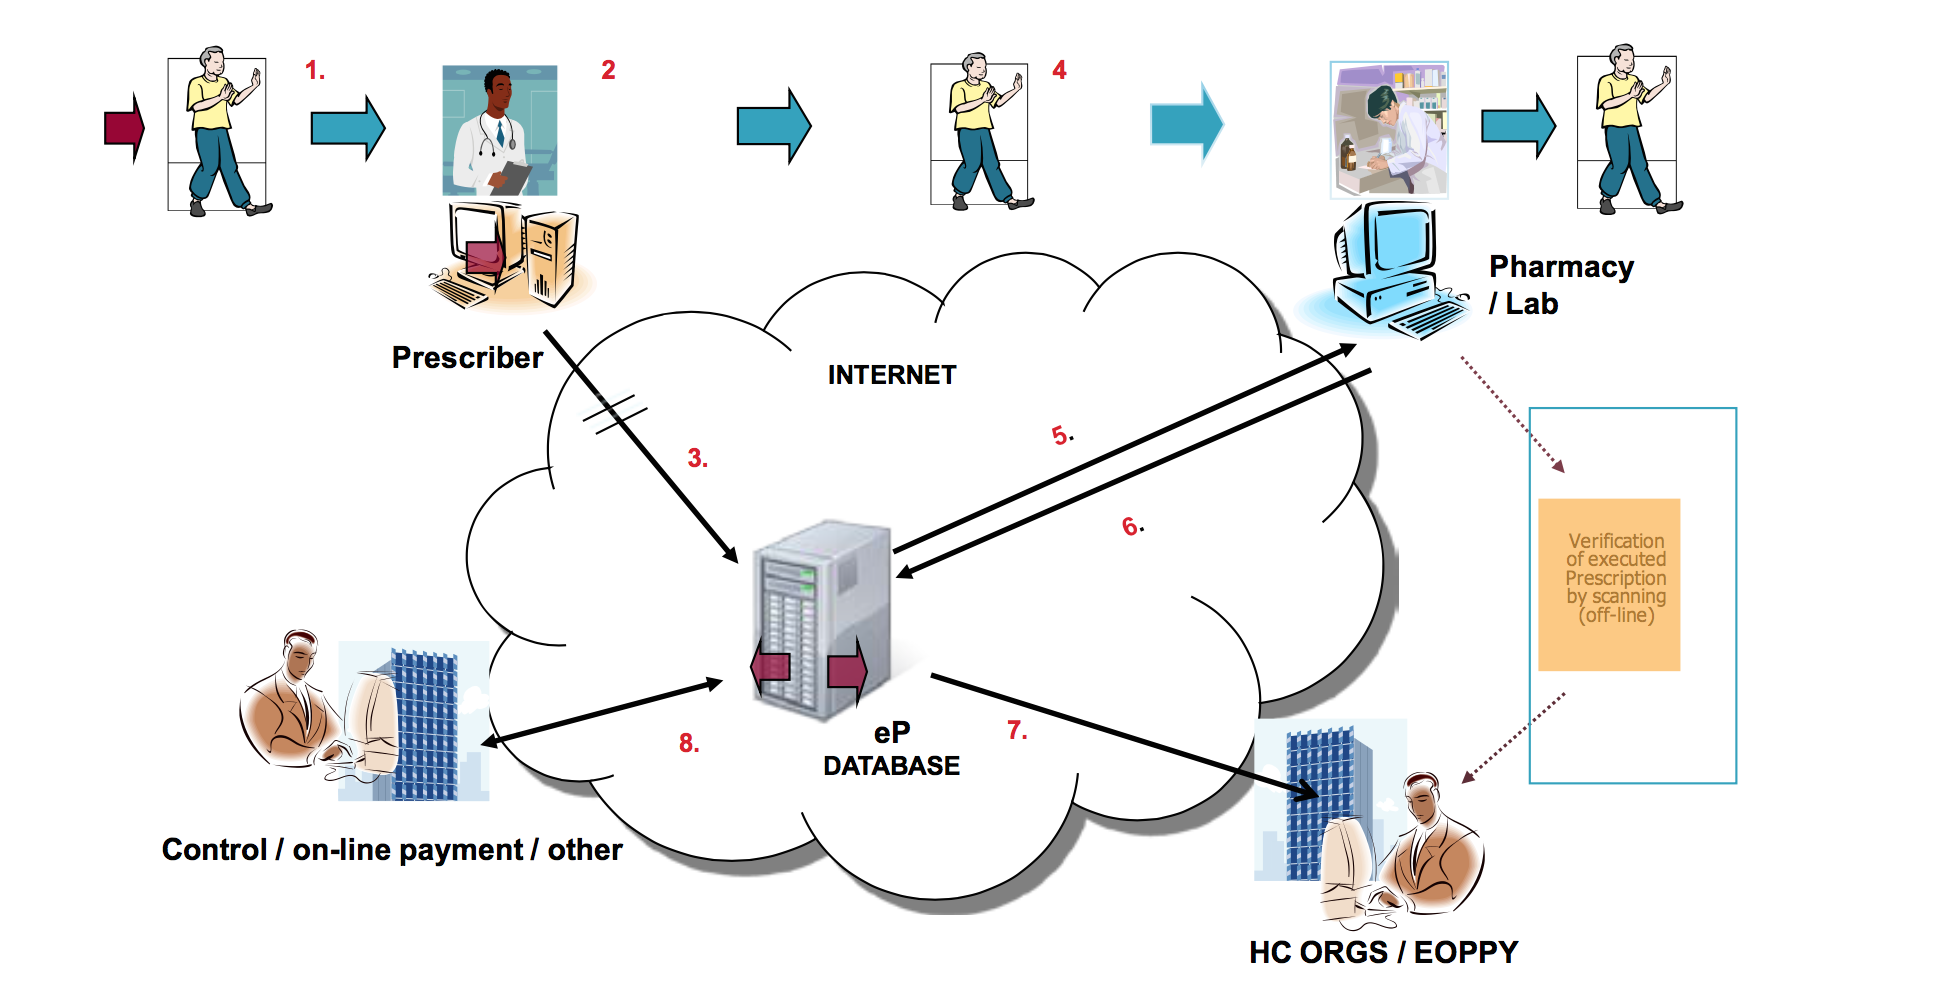
\includegraphics[width=0.7\textwidth]{e-prescr.png}
	    \caption{Το σύστημα E-prescription στην Ελλάδα. }
	    \label{fig:prescr}
	\end{figure}


	

	
	\subsection{Ηλεκτρονικός Ιατρικός Φάκελος (EMR)}
	

		Στην σύστημα υγείας η πληρότητα και η διαθεσιμότητα των δεδομένων και της πληροφορίας είναι ζωτικής σημασίας. Ημιτελείς πληροφορίες μπορούν να έχουν ως αποτέλεσμα κακή διάγνωση και θεραπεία, σπατάλη χρημάτων και πόρων ακόμα και να επιφέρουν καταστάσεις οι οποίες να απειλούν τη ζωή. Ο όγκος των πληροφοριών που σχετίζονται με την φροντίδα του ασθενούς έχει πολλαπλασιαστεί τα τελευταία χρόνια, γεγονός που οφείλεται σε μεγάλο ποσοστό στην ενσωμάτωση αυξημένου αριθμού εργαστηριακών και παρακλινικών εξετάσεων στους φακέλους των ασθενών.
	
		Ο ηλεκτρονικός ιατρικός φακέλου είναι ένα σύστημα σχεδιασμένο ώστε να υποστηρίζει την απόλυτη διαθεσιμότητα και την ακρίβεια ιατρικών ή άλλων πληροφοριών με σκοπό την παροχή ιατρικής περίθαλψης. Ο ηλεκτρονικός ιατρικός φάκελος ασθενούς είναι μία διαρκώς εξελισσόμενη έννοια και καθορίζεται ως μια συλλογή από ιατρικές πληροφορίες ιδιωτών ή πληθυσμών. Είναι αποθηκευμένος σε ψηφιακή μορφή, έχει την ικανότητα να διαμοιράζεται μεταξύ διαφορετικών ιατρικών λογισμικών και μπορεί να μεταφερθεί μέσω του δικτύου. Ένας ηλεκτρονικός φάκελος μπορεί να περιλαμβάνει μεγάλο πλήθος δεδομένων σε πλήρη ή περιληπτική μορφή, όπως δημογραφικά στοιχεία, ιατρικό ιστορικό φαρμακευτική αγωγή και αλλεργίες, προσωπικά στοιχεία όπως βάρος, ύψος, φύλο και άλλα.
		
		Σε αυτό το σημείο θα πρέπει να κάνουμε τον διαχωρισμό του ηλεκτρονικού ιατρικού φακέλου(EMR) και του ηλεκτρονικού φακέλου υγείας(EHR). O ηλεκτρονικός φάκελος υγείας (EHR) είναι μια εξελισσόμενη έννοια 
που αποθηκεύει ψηφιακά ένα υποσύνολο δεδομένων ή όλα τα δεδομένα σχετικά με τις ιατρικές πράξεις που έγιναν κατά τη διάρκεια της ζωής ενός ατόμου με σκοπό την υποστήριξη της ποιοτικής, προσβάσιμης και αποτελεσματικής συνέχειας στην παροχή υπηρεσιών υγείας. Ο ηλεκτρονικός ιατρικός φάκελος σε αντίθεση ορίζεται ως το αρχείο του ασθενούς που δημιουργήθηκε από τους παρόχους για συγκεκριμένες επισκέψεις του ασθενή σε νοσοκομεία και περιπατητική περιβάλλοντα, και η οποία μπορεί να χρησιμεύσει ως πηγή δεδομένων για τον ηλεκτρονικό φάκελο υγείας (EHR). Ο ηλεκτρονικός φάκελος υγείας (EHR) δημιουργείται και διατηρείται εντός ενός θεσμικού οργάνου, όπως ένα νοσοκομείο, ένα ολοκληρωμένο δίκτυο διανομής,μία κλινική, ή ένα γραφείο ιατρού για να δώσει σε όλους τους εμπλεκόμενους στην ιατρική φροντίδα πρόσβαση ιατρικό ιστορικό του ασθενούς.
	
	
		Ο κλασσικός ηλεκτρονικός ιατρικός φάκελος πρέπει κάθε χρονική στιγμή να περιέχει τουλάχιστον την επίσκεψη-επαφή του ασθενούς, το ιατρικό ιστορικό, τη διάγνωση, τη νοσηλεία (συνταγογράφηση, αποτελέσματα εργαστηριακών εξετάσεων ), τα δημογραφικά στοιχεία του ασθενούς (Όνομα, ΑΜΚΑ, Ασφαλιστικός φορέας, ομάδα αίματος κ.τ.λ.).


Το λογισμικό του ηλεκτρονικού φακέλου υγείας ουσιαστικά είναι ένα σύστημα διαχείρισης ιατρικών φακέλων που βασίζεται σε ηλεκτρονικούς υπολογιστές. Το γεγονός αυτό έχει ως αποτέλεσμα να αποθηκεύονται και να ανακτώνται δεδομένα γρήγορα και με ασφάλεια. Επιπλέον, τα δεδομένα επεξεργάζονται εύκολα και γρήγορα και μπορούν να μεταφερθούν σε οποιαδήποτε σύστημα, σε οποιαδήποτε απόσταση. Το σύστημα καταγραφής των δεδομένων γίνεται πιο αποτελεσματικό και περισσότερο πλήρες. Ο ηλεκτρονικός ιατρικός φάκελος εμπεριέχει μία πληθώρα δεδομένων, τα οποία έχουν διαφορετική μορφή. Το ιστορικό, η κλινική εξέταση και τα αποτελέσματα εργαστηριακών εξετάσεων, είναι σε μορφή κειμένου, οι εξετάσεις του ασθενούς (ακτινογραφίες, τομογραφίες - αξονικές, μαγνητικές, απλές - υπέρηχοι κ.α.) είναι σε μορφή στατικών εικόνων, τα ηλεκτροκαρδιογραφήματα είναι σε μορφή βιοσημάτων ,τα αποτελέσματα των ενδοσκοπικών εξετάσεων (γαστροσκόπηση κ.α. ) είναι σε μορφή βίντεο κ.λ.π.  Στον ηλεκτρονικό ιατρικό φάκελο , όλα τα δεδομένα ενσωματώνονται στον φάκελο του ασθενούς χωρίς να παίζει σημαντικό ρόλο η μορφή τους. Σε διάφορα σημεία του κειμένου του ιστορικού και της κλινικής εξετάσεως ενσωματώνονται ακτινολογικές ή βιοχημικές εξετάσεις, πράγμα που κάνει αμέσως εμφανή την συσχέτιση των εν λόγω εξετάσεων με την γενικότερη κατάσταση του ασθενούς.

Μερικά από τα πιο ουσιαστικά πλεονεκτήματα της χρήσης ενός συστήματος ηλεκτρονικού ιατρικού φακέλου είναι τα εξής
\begin{itemize}

\item Κέρδος χρόνου κατά την αναζήτηση και την συμπλήρωση στοιχείων του ιατρικού φακέλου. Η διείσδυση των τεχνολογιών αιχμής στον ιατρικό κόσμο εκσυγχρονίζεις την διαδικασία και κρατώντας όλα τα στοιχεία συγκεντρωμένα και με δυνατότητα άμεσης πρόσβασης - αναζήτησης επιταχύνουμε πολύ τις διαδικασίες.


\item

\item


\end{itemize}



Η ασφάλεια των ιατρικών δεδομένων είναι ένα σημαντικότατο θέμα για το οποίο, η
τεχνολογία μέσω του ηλεκτρονικού ιατρικού φακέλου έχει δώσει ουσιαστικές λύσεις, οι οποίες
μάλιστα μπορεί να θεωρηθούν αποτελεσματικότερες από αυτές που μέχρι σήμερα εφαρμόζονται
για την τήρηση και φύλαξη των ιατρικών φακέλων των ασθενών.
Στον ηλεκτρονικό ιατρικό φάκελο δίνεται ιδιαίτερη έμφαση στην προστασία των
προσωπικών δεδομένων τα οποία αρχειοθετούνται. Φυσικά λόγω της ευαισθησίας των
προσωπικών στοιχείων, πληρούνται όλες εκείνες οι προϋποθέσεις ασφαλείας που εξασφαλίζουν
το αδιάβλητο των δεδομένων. 


	
	
	\subsection{epSOS}
	
		Η ανάγκη διασύνδεσης των συστημάτων υγείας και των πολιτικών που ακολουθούνται σε κάθε κράτος σχετικά με την υγεία στην Ευρωπαϊκή Ένωση, γίνεται όλο και πιο πιεστική, λόγω της αυξημένης κινητικότητας των ασθενών και των επαγγελματιών του ιατρικού τομέα και της διάδοσης των νέων ιατρικών τεχνολογιών και τεχνικών που αφορούν την τεχνολογία της πληροφορίας. Η διασύνδεση των διάφορων συστημάτων υγείας είναι απαραίτητη για την καλύτερη ποιότητα αλλά και την άμεση πρόσβαση των πολιτών στη διασυνοριακή περίθαλψη.  Πολλά κράτη μέλη της Ευρωπαϊκής Ένωσης έχουν αναπτύξει ηλεκτρονικά συστήματα σχετικά με τα αρχεία των ασθενών. Ο ηλεκτρονικός ιατρικός φάκελος του ασθενούς και η ηλεκτρονική συνταγογράφηση είναι δύο πολύ σημαντικά συστήματα τα οποία προάγουν την ασφαλή και αξιόπιστη ιατροφαρμακευτική περίθαλψη.	 	
	 	
	 	Η Ευρωπαϊκή Ένωση στα πλαίσια του στόχου της επικοινωνίας και της συνεργασίας των χωρών που εντάσσονται σε αυτή και την ύπαρξη κοινών οδηγιών στον τομέα της υγείας, τον Ιούλιο του 2008 σε συνεργασία με τους δημόσιους φορείς που έχουν αρμοδιότητα τις ηλεκτρονικές υπηρεσίες υγείας (ηλεκτρονικός ιατρικός φάκελος, ηλεκτρονικής συνταγογράφησης) ξεκίνησε ένα σημαντικό έργο, τον ευρωπαϊκό πιλότο epSOS (Έξυπνες Ανοιχτές Ηλεκτρονικές Υπηρεσίες για τους Ευρωπαίους Ασθενείς). Ο κύριος στόχος του epSOS είναι η ανάπτυξη ενός πρακτικού πλαισίου ηλεκτρονικής υγείας και κατάλληλων  υποδομών  στον τομέα της  Πληροφορικής και των Επικοινωνιών που θα επιτρέπουν την ασφαλή πρόσβαση των διάφορων μη εθνικών ευρωπαϊκών συστημάτων υγειονομικής περίθαλψης στις πληροφορίες αναφορικά με την υγεία του ασθενούς. Το epSOS είναι ένα έργο για την προώθηση της δια-λειτουργικότητας της ηλεκτρονικής υγείας , το οποίο χρηματοδοτεί η Ευρωπαϊκή Ένωση και θέλει να χτίσει μια υποδομή υπηρεσιών, που θα επιτρέπει  τη διασυνοριακή διαλειτουργικότητα των συστημάτων ηλεκτρονικών μητρώων υγείας στην Ευρώπη, χωρίς να καταπατά όμως νομοθετικές ρυθμίσεις ή να υπερβαίνει τα ήδη υπάρχουσα εθνικά συστήματα. \cite{Dogac2012}


		Το epSOS αποτελείται από δύο χωριστές υπηρεσίες ηλεκτρονικής υγείας, τον ιατρικό φάκελο ασθενούς (patient medical record) και την ηλεκτρονική συνταγογράφηση (e-prescription),  για τις οποίες αναζητούνται δια-λειτουργικές μέθοδοι στη διασυνοριακή επικοινωνία. Ειδικότερα, ο ιατρικός φάκελος ασθενούς  (patient medical record) στα πλαίσια του epSOS αποτελείται από στοιχεία τα οποία εμπεριέχουν γενικές πληροφορίες για τον ασθενή (π.χ. όνομα, ηλικία, γένος), σημαντικά κλινικά δεδομένα (π.χ. αλλεργίες, χρόνιες ασθένειες, χειρουργικές επεμβάσεις) , καθώς και τα τρέχοντα αλλά και παλαιότερα φαρμακευτικά σκευάσματα που λάμβανε. Ο φάκελος ασθενούς παρέχει τις βασικές πληροφορίες, οι οποίες βοηθούν τους επαγγελματίες του τομέα της υγείας να λάβουν σωστότερες και πιο ασφαλείς αποφάσεις σχετικά με την θεραπεία και τα φάρμακα που θα ακολουθήσουν οι ασθενείς. Οι πληροφορίες αυτές πρέπει να παρέχονται στην γλώσσα των εκάστοτε γιατρών, ώστε να μην προκύπτουν γλωσσικά εμπόδια. Η ηλεκτρονική συνταγογράφηση αφορά τη συνταγογράφηση των φαρμάκων με χρήση κατάλληλου λογισμικού και την ηλεκτρονική διαβίβασή τους. Στην ηλεκτρονική συνταγογράφηση η διαλειτουργικότητα μεταξύ των εθνικών συστημάτων είναι απαραίτητη όταν έχουμε έναν ασθενή ο οποίος χρειάζεται κάποιο φάρμακο, το οποίο έχει ήδη συνταγογραφηθεί σε κάποια άλλη χώρα.  Ο φαρμακοποιός θα πρέπει να αποκτήσει ηλεκτρονική πρόσβαση στη συνταγή, και όταν το φάρμακο αγοραστεί, το ηλεκτρονικό σύστημα θα πρέπει να ενημερώσει σχετικά με τα διανεμημένα φάρμακα το σύστημα υγειονομικής περίθαλψης της χώρας του ασθενούς. \cite{epSOS}
		
		 Το epSOS επιτυγχάνει την ασφαλή πρόσβαση των ασθενών σε πληροφορίες σχετικά με την υγεία τους για τα διάφορα ευρωπαϊκά συστήματα υγείας. Το σύστημα είναι φτιαγμένο για να εξυπηρετήσει έναν πολίτη της Ευρωπαϊκής Ένωσης  που ενώ είναι κατοικεί σε μια συγκεκριμένη χώρας δέχεται τακτικά υπηρεσίες υγείας σε μια άλλη χώρα εξαιτίας του καθώς εργάζεται σε αυτή τη χώρα ή βρίσκεται προσωρινά σε μία άλλη χώρα (π.χ. για τουρισμό ) και είναι ανάγκη να εκτελέσει μία ιατρική συνταγή της χώρας του ή χρειάζεται επείγουσα ιατρική περίθαλψη. Το epSOS παρέχει την κοινοτική οδηγία για τη διασυνοριακή ιατρική περίθαλψη, η οποία θα πρέπει να ενσωματωθεί στο εθνικό δίκαιο των κρατών μελών τα επόμενα χρόνια και επιπροσθέτως προτείνει τεχνικές λύσεις σε όλα τα επίπεδα δια-λειτουργικότητας, όπως και σε θέματα πολιτικής και σε νομικά ζητήματα. επεκτείνεται πέρα από την έκδοση συστάσεων, μοντέλων οργάνωσης, και εργαλείων λογισμικού  στην  δοκιμή των αποτελέσματα αυτών μέσω πραγματικών πιλοτικών εφαρμογών σε πολλές ευρωπαϊκές περιφέρειες και χώρες.
		 


\section{Eligibility as a Service}

			\subsection{Motivation}
			
						
			Η πρωταρχική ευθύνη της υπηρεσίας μετάγγισης αίματος είναι να παρέχει ένα ασφαλές και
επαρκές απόθεμα αίματος και προϊόντων που παράγονται από το αίμα. Θα πρέπει να διασφαλίζεται ότι τα προϊόντα που προέρχονται από δωρεές αίματος παρουσιάζουν ελάχιστο κίνδυνο ύπαρξης οποιασδήποτε μόλυνσης, που θα μπορούσε να μεταδοθεί μέσω μετάγγισης. Όλοι οι υποψήφιοι αιμοδότες αξιολογούνται για την καταλληλότητά τους να δωρίσουν αίμα, σε κάθε περίπτωση δωρεάς. 
		
		Οι βασικές φάσεις ελέγχου του αίματος είναι οι εξής:
		\begin{itemize}
		\item	Φάση 1: Συμπλήρωση χειρόγραφου ερωτηματολογίου σχετικά με ιστορικό υγείας του ασθενούς.
		\item Φάση 2: Εξέταση του εθελοντή αιμοδότη από ιατρό και βασικές εξετάσεις (μέτρηση πίεσης, έλεγχος αιμοσφαιρίνης) και ερωτήσεις σχετικά με το ιατρικό ιστορικό του αιμοδότη.
		\item 	Φάση 3: Μετά την αιμοληψία, το αίμα περνάει μοριακούς και μικροβιολογικούς ελέγχους.
		\end{itemize}		 
		
		Οι πληροφορίες που παρέχονται από 164 χώρες για την παγκόσμια Βάση Δεδομένων για την ασφάλεια αίματος δείχνουν ότι, συλλέγονται περισσότερες από 92 εκατομμύρια αιμοδοσίες ετησίως. Επιπλέον, τουλάχιστον 13 εκατομμύρια υποψήφιοι δότες απορρίπτονται πριν προλάβουν να φτάσουν στην αιμοληψία, δηλαδή στις φάσεις 1,2. \cite{safety} Οι λόγοι απόρριψης των φάσεων 1, 2 , τους οποίους θα εξετάσουμε στην παρούσα διπλωματική, έχουν να κάνουν με το ιατρικό ιστορικό του ασθενή (χρόνιες ασθένειες, αλλεργίες κ.λ.π.), με υπάρχουσες ιατρικές καταστάσεις (λοιμώξεις, λήψη αντιβίωσης, λήψη φαρμάκων που σε καθιστούν ακατάλληλο για  αιμοδοσία κ.λ.π.) και με καταστάσεις της προσωπικής ζωής του εθελοντή (π.χ. ομοφυλοφιλία). Το υπερβολικά μεγάλο ποσοστό απορρίψεων 14.13\% τονίζει την ανάγκη να μειωθεί ο αριθμός των περιπτώσεων της προσωρινής απόρριψης (με τον όρο προσωρινή απόρριψη, αναφερόμαστε σε προσωρινή αναβολή της αιμοδοσίας που συμβαίνει στις φάσεις 1, 2 λόγω προσωρινής ακαταλληλότητας των δοτών).

		Το ποσοστό αυτό, γίνεται ιδιαίτερα σημαντικό και ζημιογόνο οικονομικά να κάνουμε μία ανάλυση των επιμέρους κοστών της αιμοδοσίας. Τα κόστη της αιμοδοσίας είναι ιδιαίτερα υψηλά. Θα παρουσιάσουμε την μέση τιμή αυτών των κοστών, όπως υπολογίσθηκε από το ελληνικό Υπουργείο Υγείας,το 2011.\cite{Fragoulakis} Στα κόστη περιλαμβάνεται το κόστος μηχανογράφησης (απογραφή και συντήρηση) των κέντρων αίματος, η τιμή των διαφόρων τύπων εξοπλισμού, το υπόλοιπο του κύκλου ζωής (που μετράται σε έτη) για τον ιατρικό εξοπλισμό. Επίσης, μετρώνται τα πάγια κόστη των μονάδων, τα οποία σχετίζονται με την ηλεκτρική ενέργεια,  τον καθαρισμό, την ασφάλεια, την διαχείριση, και όλες τις άλλες υποστηρικτικές υπηρεσίες που διατίθενται για τα κέντρα αίματος. Στον πίνακα \ref{tab:costs} αναφέρονται αναλυτικά τα κόστη, των φάσεων 1 και 2 για την συλλογή 1 μονάδας αίματος στην Ελλάδα.
		
		
		%na ftiaksoume to table 
		\begin{table}[H]
	\centering
	\begin{tabular}{l|}

	\end{tabular}
	\caption{Συνολικό κόστος για την συλλογή 1 μονάδας αίματος στην Ελλάδα.}
	\label{tab:costs}
\end{table}
		
		Παρατηρούμε ότι το συνολικό κόστος για είναι 98.07 € ανά μονάδα αίματος.  Με βάση το ποσοστό 14.13\%, σε μία γενική περίπτωση στις 100 αιμοδοσίες έχουμε 9,807 € έξοδα. Τα 1,385.73 €, είναι έξοδα για περιπτώσεις στις οποίες δεν θα πραγματοποιηθεί ποτέ αιμοληψία. Σε αυτό το σημείο πρέπει να τονίσουμε, ότι δεν έχουν συμπεριληφθεί όλα τα κόστη στην μελέτη μας, παρά μόνο τα απολύτως διακριτά και ξεκάθαρα μετρήσιμα.
	
		Πέραν του οικονομικού μέρους, μια άλλη πολύ σημαντική παράμετρος είναι η άσκοπη κατανάλωση χρόνου τόσο του ιατρικού προσωπικού του αιμοδοτικού κέντρου, όσο και των εθελοντών αιμοδοτών. Οι εθελοντές αιμοδότες καταναλώνουν αρκετό χρόνο για τον προγραμματισμό, την μετάβαση στο αιμοδοτικό κέντρο, την αναμονή και για την διαδικασία αιμοδοσίας.  Δεδομένου ότι το μεγαλύτερο ποσοστό είναι εργαζόμενοι, ο χρόνος αυτός είναι σημαντικός και είναι επιθυμητό να αποφευχθεί η περιττή ταλαιπωρία που προκύπτει για τους δωρητές λόγω προσωρινής τους απόρριψης. Η μείωση των περιπτώσεων προσωρινής απόρριψης, θα εξασφαλίσει μείωση της σπατάλης του χρόνου του προσωπικού.
		
		Μία επιπλέον πολύ σημαντική παράμετρος αποτελεί το ποσοστό επιστροφής των εθελοντών αιμοδοτών μετά από μία προσωρινή απόρριψη. Μελέτες έχουν δείξει ότι οι περισσότεροι εθελοντές δεν επιστρέφουν αν απορριφθούν μία φορά. Πιο συγκεκριμένα, ..... %να διαβασω papers 
	
		
		
		
		
		
\section{Δοκιμές}

\chapter{Συζήτηση - Επεκτάσεις}\label{ch:Discussion}
\section{SmartWatch}
\section{DSS για απόρριψη ασθενή}
\section{Predictive Analytics Subsystem}
\section{Real-Time Inventory Reporting}


\chapter{Επίλογος}\label{ch:conclusion}

\section{Τελικές Παρατηρήσεις}

\section{Μελλοντική δουλειά}



%%%  Bibliography

\bibliographystyle{softlab-thesis}
\bibliography{references}


%%%  Appendices

\backmatter

\appendix

\chapter{Ευρετήριο συμβολισμών}

$A \rightarrow B$ : συνάρτηση από το πεδίο $A$ στο πεδίο $B$.

\chapter{Ευρετήριο γλωσσών}

\textbf{Haskell} : η γλώσσα της ζωής μου.

\chapter{Ευρετήριο αριθμών}

42 : life, the universe and everything.


%%%  End of document

\end{document}
